\documentclass{report}
\usepackage[spanish]{babel}
\usepackage[utf8x]{inputenc}



\usepackage{amsmath,amsthm}
\usepackage{amsmath}
\usepackage{amssymb}
\usepackage{amsfonts}
\usepackage{amsthm}
\usepackage{amsbsy}
\usepackage{amsgen}
\usepackage{amscd}
\usepackage{amsopn}
\usepackage{amstext}
\usepackage{amsxtra}
\usepackage{mathrsfs}
\usepackage{enumitem}
\usepackage{graphicx}
\usepackage{verbatim}
\usepackage{epstopdf}
\usepackage{float}
\usepackage[all,cmtip]{xy}
\usepackage{accents}
\usepackage{sseq}
\usepackage{url}
\usepackage{hyperref}
\usepackage{makeidx}
%\usepackage{tikz}
\usepackage{wrapfig}
\usepackage{tikz-cd}
\usepackage{framed,enumitem} 
\usepackage{syllogism}
\usepackage{bussproofs} 
% ^ este es para hacer reglas de inferencia. 
\usepackage{xfrac}
\usepackage{collectbox}%Para hacer cajitas de algoritmos


\usetikzlibrary{matrix, positioning}
\usepackage[T1]{fontenc}
\usepackage{titlesec, blindtext, color}
\definecolor{gray75}{gray}{0.75}
\newcommand{\hsp}{\hspace{20pt}}
\titleformat{\chapter}[hang]{\Huge\bfseries}{\thechapter\hsp\textcolor{gray75}{|}\hsp}{0pt}{\Huge\bfseries}

\newtheorem{theorem}{Teorema}[chapter]
\newtheorem{theorem*}[theorem]{*Teorema}
\newtheorem{prop}[theorem]{Proposición}
\newtheorem{lema}[theorem]{Lema}
\newtheorem{cor}[theorem]{Corolario}

\newtheorem{prop*}[theorem]{*Proposición}
\newtheorem{lema*}[theorem]{*Lema}
\newtheorem{cor*}[theorem]{*Corolario}

\theoremstyle{definition}
\newtheorem{definition}[theorem]{Definición}
\newtheorem{definition*}[theorem]{*Definición}
\newtheorem{defs}[theorem]{Definiciones}
\newtheorem{defs*}[theorem]{*Definiciones}
\newtheorem{example}[theorem]{Ejemplo}
\newtheorem{ex}[theorem]{Ejercicio}
\newtheorem{note}[theorem]{Nota}

\theoremstyle{remark}
\newtheorem{remark}[theorem]{Nota}

\newtheoremstyle{jeje} % name
    {\topsep}                    % Space above
    {\topsep}                    % Space below
    {}                   % Body font
    {}                           % Indent amount
    {\itshape}                   % Theorem head font
    {.}                          % Punctuation after theorem head
    {.5em}                       % Space after theorem head
    {}  % Theorem head spec (can be left empty, meaning ‘normal’)
\theoremstyle{jeje}
\newtheorem*{sketchproof}{Sketch de demostración}

\DeclareMathOperator{\Tr}{Tr}
\newcommand{\N}{\mathbb{N}}
\newcommand{\Q}{\mathbb{Q}}
\newcommand{\R}{\mathbb{R}}
\newcommand{\K}{\mathbb{K}}
\newcommand{\norm}[1]{\left\|#1\right\|}
\newcommand{\dv}[3]{\frac{\partial #1}{\partial #2}(#3)}


\newcommand{\T}{\mathbb{T}}
\renewcommand{\P}{\mathbb{P}}
\newcommand{\C}{\mathbb{C}}
\renewcommand{\H}{\mathbb{H}}
\newcommand{\Z}{\mathbb{Z}}
\newcommand{\F}{\mathbb{F}}
\newcommand{\tr}{\mathrm{tr}}
\newcommand{\idash}{\quad}

%Para poner gorritos:
\usepackage{scalerel,stackengine}
\stackMath
\newcommand\reallywidehat[1]{%
\savestack{\tmpbox}{\stretchto{%
  \scaleto{%
    \scalerel*[\widthof{\ensuremath{#1}}]{\kern.1pt\mathchar"0362\kern.1pt}%
    {\rule{0ex}{\textheight}}%WIDTH-LIMITED CIRCUMFLEX
  }{\textheight}% 
}{2.4ex}}%
\stackon[-6.9pt]{#1}{\tmpbox}%
}

%Para poner diagramas:
\usetikzlibrary{matrix,arrows,decorations.pathmorphing}
\tikzset{commutative diagrams/.cd}


\def\regla#1{\ensuremath\mathbf{(#1)}}

%Para poner cajitas en los algoritmos:
\makeatletter
\newcommand{\sqbox}{%
    \collectbox{%
        \@tempdima=\dimexpr\width-\totalheight\relax
        \ifdim\@tempdima<\z@
            \fbox{\hbox{\hspace{-.5\@tempdima}\BOXCONTENT\hspace{-.5\@tempdima}}}%
        \else
            \ht\collectedbox=\dimexpr\ht\collectedbox+.5\@tempdima\relax
            \dp\collectedbox=\dimexpr\dp\collectedbox+.5\@tempdima\relax
            \fbox{\BOXCONTENT}%
        \fi
    }%
}
\makeatother










\numberwithin{section}{chapter}
\numberwithin{equation}{chapter}

\makeindex

\begin{document}



\title{Apuntes de\\ Lógica Matemática}


\author{Saúl Rodríguez Martín\\ Miguel Muñoz Pérez \\ Eduardo González Vaquero}

\maketitle




%    Dedication.  If the dedication is longer than a line or two,
%    remove the centering instructions and the line break.
\cleardoublepage
\vspace*{13.5pc}
\begin{center}
  Apuntes basados en las clases de Luis Fernando Llana Díaz de la asignatura Lógica Matemática del grado en Matemáticas de la Universidad Complutense de Madrid. Redactados durante el curso académico 2019-2020.\\
  Se agradece el envío de erratas a saulro01@ucm.es.\\
  Gracias a Alberto Acosta por señalar numerosas erratas.
\end{center}
\cleardoublepage

%    Change page number to 6 if a dedication is present.

\tableofcontents
\pagenumbering{gobble}

%    Include unnumbered chapters (preface, acknowledgments, etc.) here.



%    Include main chapters here.

\chapter{Lógica proposicional}
\\
\section{Introducción}
Antes de comenzar con definiciones rigurosas, conviene dar una breve explicación sobre la motivación de la lógica proposicional, a la que dedicaremos este capítulo. Un aspecto común de los lenguajes naturales (como el español o el chino) es la ambigüedad de ciertas expresiones, lo cual dificulta las intenciones usuales de la ciencia, a saber, la precisión en la comunicación y la distinción clara de aquello que se comunica. De aquí nace una necesidad evidente, que es cubierta por los lenguajes artificiales y, entre ellos, la lógica formal. \

Debemos aclarar entonces cuál es nuestro objeto de estudio. Fijémonos en lo siguiente: existen ciertos elementos del lenguaje que no cambian si los traducimos a otro idioma, por ejemplo. Nos referimos a lo que se denomina como \textit{conectivas lógicas}, es decir, `no' (negación), `o' (disyunción), `y' (conjunción), `si... entonces' (implicación material) y `si y solo si' (equivalencia). Obviamente, podemos usar múltiples expresiones distintas para referirnos a cada una de ellas, pero su función en el lenguaje natural no cambia. Por esto mismo podemos formalizarlas y estudiarlas desde el punto de vista matemático.  

Ahora bien, a fin de sistematizar nuestro lenguaje, introducimos una serie de símbolos que se referirán a las entidades correspondientes del lenguaje natural. Conviene puntualizar de nuevo que estas traducciones, es decir, estas `asignaciones de significados' \textit{no} son únicas. Esto lo veremos más adelante. Entonces tenemos: $\neg$ (negación), $\lor$ (disyunción), $\land$ (conjunción), $\rightarrow$ (implicación material) y $\leftrightarrow$ (equivalencia). \

Los otros elementos básicos que constituirán nuestro lenguaje formal son las \textit{proposiciones}. Con el fin de no entrar en cuestiones semánticas que exceden nuestro estudio, establecemos la siguiente:

\begin{definition}\label{def: prop}
    Una proposición es un enunciado que puede ser verdadero o falso. 
\end{definition}
Como con las conectivas, introducimos una serie de \textit{símbolos de proposición} para referirnos formalmente a las proposiciones. Denotamos por $SP$ al conjunto de todos estos símbolos.

Así, el enunciado `Todos los solteros son hombres no casados' es una proposición, mientras que `¿Va a llover mañana?' no lo es. Por otro lado, `César conquistó las Galias y combatió contra Vercingétorix' admite una descomposición como conjunción de dos proposiciones. Evidentemente, esta reducción a proposiciones más simples tiene que parar eventualmente; así llegamos a lo que denominamos \textit{proposiciones atómicas}. Esto nos permitirá, una vez determinada la verdad o falsedad de estas proposiciones atómicas, hallar la de todas las proposiciones que se compongan de ellas mediante la aplicación de las conectivas lógicas (antiguamente llamadas \textit{proposiciones moleculares}). \

Las proposiciones atómicas se representan entonces por los elementos de $SP$. Añadimos, por motivos que serán aclarados más adelante, dos elementos $\top$ y $\bot$, que se refieren a la \textit{proposición idénticamente verdadera} y a la \textit{proposición idénticamente falsa}, respectivamente. Es decir, 

\begin{definition}\label{def : at}

     Definimos el conjunto de las proposiciones atómicas como:
    \[
        AT := SP\cup \{\top, \bot\}
    \]
\end{definition}


\begin{definition}(Alfabeto)
    Dado un conjunto de símbolos de proposiciones $SP$, se denomina alfabeto a:
    \[
        A_{SP} = SP\cup\{\neg, \land, \lor, \rightarrow, \leftrightarrow, (, ),\top, \bot\},
    \]
    obtenido añadiendo a $SP$ las conectivas lógicas $\neg, \land, \lor, \rightarrow, \leftrightarrow$, y los paréntesis, $(,)$.
\end{definition}    

\begin{definition}(Cierre de Kleene)
    Dado un conjunto de símbolos $A$, definimos el cierre de Kleene de $A$, $A^*$, como el conjunto de las concatenaciones de elementos de $A$ junto con $\epsilon$, el \textit{espacio vacío} o en blanco.
\end{definition}

\begin{example} Dado $A = \{a, b\}$, le corresponde 
\[
    A^* = \{\epsilon, a, b, ab, ba, aab, baa, aba, ...\}
\]
\end{example}
\begin{example}
    $A_{SP}^*$ será el conjunto de todas las concatenaciones de elementos de $A_{SP}$, junto con $\epsilon$.
\end{example}

Una vez que disponemos de los elementos básicos de la sintaxis del lenguaje y sus sucesivas combinaciones, nos interesa definir las expresiones que están `bien formadas', es decir, queremos excluir de nuestro lenguaje  concatenaciones de símbolos como `$)) \leftrightarrow \varphi$'.

\begin{definition}\label{def:PROP_{SP}}(Proposiciones posibles)
Se define el conjunto de proposiciones posibles,  $PROP_{SP}$, como la intersección de todos los subconjuntos de $A_{SP}^*$ que verifican:
\begin{enumerate}
    \item $SP \subseteq PROP_{SP}$.
    \item Si $\phi\in PROP_{SP}$, entonces $(\neg \phi) \in PROP_{SP} $.
    \item Si $\phi_1, \phi_2 \in PROP_{SP}$ y $\square\in \{\land, \lor, \rightarrow, \leftrightarrow\}$, entonces $(\phi_1 \square\  \phi_2) \in PROP_{SP}$.
\end{enumerate}
\end{definition}
Es fácil comprobar que $PROP_{SP}$ también cumple estas tres propiedades, por tanto decimos que es el mínimo subconjunto que las verifica.

\begin{prop} Se define $P_0 := SP$ y para cada $n\in\N$:
\[
    P_n := P_{n-1} \cup \{(\neg \phi): \phi\in P_{n-1}\}\cup \{ (\phi_1 \square\  \phi_2): \phi_1, \phi_2\in P_{n-1},  \square\in \{\land, \lor, \rightarrow, \leftrightarrow\}\}.
\]
Entonces $P := \bigcup_{n=0}^\infty P_n$ coincide con $PROP_{SP}$.
\begin{proof} 
Comenzamos comprobando $P\subseteq PROP_{SP}$. Para ello, comprobamos por inducción que $P_n\subseteq PROP_{SP}$ $\forall n \in \mathbb{N}$. \\ \\
Está claro que $P_0\subseteq PROP_{SP}$, ya que $PROP_{SP}$ cumple la propiedad 1.
Ahora, suponiendo que $P_n\subseteq PROP_{SP}$, por las propiedades 2 y 3, $\{(\neg \phi): \phi\in P_{n-1}\}\cup \{ (\phi_1 \square\  \phi_2): \phi_1, \phi_2\in P_{n-1},  \square\in \{\land, \lor, \rightarrow, \leftrightarrow\}\}$ también estarán  contenidos en $PROP_{SP}$. Por tanto, $P_{n+1}\subseteq PROP_{SP}$, y hemos acabado la inducción. \\ \\
Veamos ahora que $PROP_{SP}\subseteq P$. Para ello nos basta comprobar que $P$ cumple las tres propiedades de la definición ~\ref{def:PROP_{SP}}. La propiedad $1$ es directa, pasamos a comprobar las propiedades 2 y 3. \\ \\
Dado $\varphi \in P$, existe $n\in \N\cup\{0\}$ tal que $\varphi \in P_n$ luego $(\neg \varphi) \in P_{n+1}$ por lo que $(\neg\varphi) \in P$. \\ \\
Sean $\varphi_1, \varphi_2 \in P$ y sea $\square\in \{\land, \lor, \rightarrow, \leftrightarrow\}$. Tomamos $n\in\N$ tal que $\varphi_1, \varphi_2 \in P_n$ (para cada uno existe al menos un natural: basta tomar el mayor). Luego $(\phi_1 \square\  \phi_2)\in P_{n+1}$ y por lo tanto también pertenece a $P$. \\ \\
\end{proof}
\end{prop}
A partir de ahora, usaremos para mayor brevedad el símbolo $\square$ como intercambiable por $\land, \lor, \rightarrow$ o $\leftrightarrow$.\\
\section{Inducción estructural y recursión}

El método de inducción nos servirá para demostrar que todas las fórmulas cumplen una \textit{propiedad}\footnote{No hemos definido rigurosamente el concepto de "propiedad", pero esencialmente significa algo que las proposiciones pueden cumplir o no. Una forma rigurosa de definir propiedad consiste en definirla como un subconjunto $P\subseteq PROP_{SP}$, de modo que decimos que una proposición cumple la propiedad $P$ si y solo si pertenece a $P$.} en dos pasos: demostrar que todas las proposiciones atómicas cumplen dicha propiedad, y demostrar que si dos proposiciones $\varphi_1,\varphi_2$ cumplen una propiedad, entonces $(\neg\varphi_1)$ y $(\varphi_1\square\varphi_2)$ también la cumplen.$\\$

\begin{prop} (Inducción estructural) Supongamos que queremos probar $P(\varphi)$ para todo $\varphi\in PROP_{SP}$ (siendo $P$ una propiedad cualquiera) entonces basta comprobar que:
\begin{enumerate}
    \item $P(\varphi)$ para toda $\varphi\in AT$.
    \item Si $P(\varphi)$ entonces $P((\neg \varphi))$.
    \item Si $P(\varphi_1)$ y $P(\varphi_2)$ entonces $P((\varphi_1 \square \varphi_2))$.
\end{enumerate}
\begin{proof}
Si una propiedad $P$ cumple estas tres propiedades, entonces el conjunto de proposiciones que cumplen $P$ cumple las tres propiedades de ~\ref{def:PROP_{SP}}, por tanto contiene a $PROP_{SP}$. \\
\end{proof}
\end{prop}

\begin{example} Definamos $P(\varphi)$ como la propiedad de $|\varphi|_) = |\varphi|_($ siendo $|\varphi|_)$ la cantidad de $)$ en la fórmula $\varphi$ y $|\varphi|_($ la cantidad de $($. Vamos a comprobar por inducción estructural que todas las proposiciones cumplen esta propiedad:
\begin{enumerate}
    \item Para cualquier $\varphi\in AT$ se verifica trivialmente $|\varphi|_) = |\varphi|_( = 0$, luego $P(\varphi)$.
    \item Supongamos $P(\varphi)$ con $\varphi\in PROP_{SP}$, entonces $|\varphi|_( = |\varphi|_)$ y por tanto:
    \[
        |(\neg\varphi)|_( = |\varphi|_(+1 = |\varphi|_)+1 = |(\neg\varphi)|_)
    \]
    luego $P((\neg\varphi))$.
    \item Supongamos $P(\varphi),P(\psi)$ con $\varphi,\psi\in PROP_{SP}$, entonces:
    \[
        |(\varphi\square\psi)|_(=|\varphi|_(+|\psi|_(+1=|\varphi|_)+|\psi|_)+1=|(\varphi\square\psi)|_)
    \]
    luego $P((\varphi\square\psi))$.
\end{enumerate}
\end{example}

\begin{definition} (Prefijos) Sea $A$ un alfabeto y sea $w\in A^*$. Decimos que $w'$ es prefijo de $w$ si existe $w''$ tal que $w = w' w''$, es decir, si $w = w_1 w_2 ... w_n$ entonces existe $0\leq k\leq n$ tal que $w' = w_1 ... w_k$.$\\$
Decimos además que un prefijo $w'$ es prefijo propio de $w$ si es distinto de $w$ y $\epsilon$.
\end{definition}

\begin{example} Sea $A := \{a, b\}$ y sea $w := aababb$. Entonces sus prefijos son $\epsilon,a,aa,aab,aaba,aabab,aababb$, correspondientes a $k=0,1,2,3,4,5,6$, respectivamente, y sus prefijos propios son $a,aa,aab,aaba,aabab$.
\end{example}

\begin{prop} Si $\varphi'$ es prefijo propio de $\varphi$, entonces $|\varphi'|_) < |\varphi'|_($.
\begin{proof} Se demuestra por inducción estructural.
\begin{enumerate}
    \item Si $\varphi\in AT$ no tiene prefijos propios luego se cumple la afirmación.
    \item Sea $\varphi\in PROP_{SP}$ cumpliendo la propiedad del enunciado y sea $\varphi'$ un prefijo propio de $(\neg \varphi)$. Existen cuatro casos:
    \begin{enumerate}
        \item $\varphi' = ($, entonces $|\varphi'|_( = 1 > 0 = |\varphi'|_)$-
        \item $\varphi' = (\neg$, ocurre lo mismo que antes.
        \item $\varphi' = (\neg \varphi''$ con $\varphi''$ prefijo propio de $\varphi$ entonces por inducción se verifica $|\varphi''|_) < |\varphi''|_($. Ahora bien, $|\varphi'|_( = |\varphi''|_(+1$  y $|\varphi'|_) = |\varphi''|_)$ luego:
        \[
            |\varphi'|_) < |\varphi'|_(
        \]
        \item $\varphi' = (\neg \varphi$, que es directo. 
    \end{enumerate}
    \item Se hace de forma similar al apartado anterior. Basta probar con los prefijos $(,\ (\varphi_1',\ (\varphi_1,\ (\varphi_1\square,\ (\varphi_1\square\varphi_2'$ y $(\varphi_1\square\varphi_2$.
\end{enumerate}
    
\end{proof}
\end{prop}

 En breve nos será útil, dado un conjunto $A$, poder definir una función $H: PROP_{SP} \rightarrow A$ conociendo su restricción a $AT$, y suponiendo que podemos calcular $H((\neg \varphi))$ y $H((\varphi\square\psi))$ en función de $H(\varphi)$ y $H(\psi)$.
 Si la función $H$ queda bien definida así, diremos que está \textit{definida de forma recursiva}. La siguiente proposición nos garantiza que podemos definir funciones de esta forma:
 
 \begin{prop} El esquema de definición recursiva da como resultado una única función, es decir, dadas:
\begin{enumerate}
    \item $H_{AT}: AT \rightarrow A$.
    \item $H_{\neg}: A \rightarrow A$.
    \item $H_{\square}: A \times A \rightarrow A$.
\end{enumerate}
existe una única función $H: PROP_{SP} \rightarrow A$ tal que:
\begin{enumerate}
    \item $H(\varphi) = H_{AT}(\varphi)$, para toda $\varphi \in AT$.
    \item $H((\neg \varphi)) = H_{\neg}(H(\varphi))$.
    \item $H((\varphi_1 \square \varphi_2)) = H_{\square}(H(\varphi_1), H(\varphi_2))$, para cada $\square\in \{\land, \lor, \rightarrow, \leftrightarrow\}$.
\end{enumerate}
\begin{proof}
     Se omite la demostración.
\end{proof}
\end{prop}

\begin{example} Sea $H: PROP_{SP} \rightarrow \mathbb{N}$ la función $|.|_($ definida anteriormente. Podemos definirla de manera recursiva:
\begin{enumerate}
    \item $H(\varphi) = 0$, para toda $\varphi \in AT$.
    \item $H((\neg \varphi)) = H(\varphi) + 1$.
    \item $H((\varphi_1 \square \varphi_2)) = H(\varphi_1) + H(\varphi_2) + 1$.
\end{enumerate}
Nótese como en ocasiones omitimos las funciones auxiliares y usamos la notación $H$ para referirnos a $H$, $H_{AT}$, $H_{\neg}$ y $H_{\square}$. Este abuso de notación no suele dar lugar a confusión.
\end{example}

\begin{ex} Definir resursivamente una función que nos lleve cada fórmula al número de veces que $\land$ aparece en ella. 
\end{ex}

\begin{example} Podemos definir una función que nos lleve cada fórmula al conjunto de todas sus subfórmulas, es decir,  $\text{\textit{\text{\textit{SUB}}}}: PROP_{SP} \rightarrow \mathcal{P} (PROP_{SP})$\footnote{Dado un conjunto X, denotamos por $\mathcal{P}(X)$ a su potencia, es decir, el conjunto de subconjuntos de X.} tal que:
\begin{enumerate}
    \item $\text{\textit{SUB}}(\varphi) = \{\varphi\}$, para toda $\varphi \in AT$.
    \item $\text{\textit{SUB}}((\neg \varphi)) = \text{\textit{SUB}}(\varphi) \cup \{(\neg \varphi)\}$.
    \item $\text{\textit{SUB}}((\varphi_1 \square \varphi_2)) = \text{\textit{SUB}}(\varphi_1) \cup \text{\textit{SUB}}(\varphi_2) \cup \{(\varphi_1 \square \varphi_2)\}$.
\end{enumerate}
\end{example} 

\section{Eliminación de paréntesis}
Para conseguir una notación más compacta, podemos establecer una notación que use menos paréntesis cuando nos convenga. Sin embargo, la omisión de paréntesis puede dar lugar a ambigüedades en las fórmulas, por ejemplo:
\[p\to q \to r\]
podría simbolizar dos fórmulas distintas:
\begin{enumerate}[label=\bullet]
    \item $((p\to q)\to r)$
    \item $(p\to (q\to r))$
\end{enumerate}
Para evitar este tipo de situaciones, necesitamos las siguientes reglas de omisión de paréntesis:
\begin{enumerate}
    \item Los paréntesis externos pueden omitirse. Esto no da lugar a ambigüedad.
    \item Las conectivas se aplicarán en este orden: $\neg, \land, \lor, \to, \leftrightarrow$.
    \item Cuando hay varias conectivas del mismo tipo seguidas, se asocia siempre por la izquierda\footnote{Cuando veamos semántica, comprobaremos que todas las conectivas salvo $\rightarrow$ son asociativas, por tanto, en ese sentido, no importa el orden en que se asocien estas conectivas.}.
\end{enumerate}
Algunos ejemplos de aplicación de estas reglas:$\\[8pt]$
\begin{equation*}
\begin{array}{ccc}
     \neg p\lor p  & \text{es} & ((\neg p)\lor p)\\
     \neg p\land q\lor s\to t\leftrightarrow r & \text{es} & 
     (((((\neg p)\land q)\lor s)\to t)\leftrightarrow r)\\
     p\to q\to s & \text{es} & ((p\to q)\to s)\\
     p\land q\leftrightarrow\neg s\to t\lor r & \text{es} & ((p\land q)\leftrightarrow((\neg s)\to (t\lor r))) \\
     t\leftrightarrow p\to \neg q\lor p\to s & \text{es} & 
     (t \leftrightarrow((p\to ((\neg q)\lor p))\to s))
\end{array}
\end{equation*}


\section{Asignaciones de verdad}

Hasta ahora hemos venido considerando cuestiones sintácticas sobre las fórmulas. Lo que queremos ahora es abordar su semántica, esto es, su comportamiento cuando les damos una interpretación determinada. Nos interesa, por tanto, estudiar qué significa que una proposición se siga de otra independientemente de la traducción que hagamos al lenguaje natural, esto es, la noción de \textit{consecuencia lógica}. Así, por ejemplo, queremos que $q$ se siga de $p \land (p \rightarrow q)$ independientemente de cómo se traduzcan $p$ y $q$ informalmente. Es decir, exigimos que, sea cual sea la traducción de $p \land (p \rightarrow q)$, si es verdadera entonces la de $q$ tiene que serlo también.  Siguiendo la definición ~\ref{def: prop}, 

\begin{definition}
Definimos el conjunto de valores de verdad, $Bool = \{V, F\}$, donde $V$ es \textit{la verdad} y $F$ es \textit{la falsedad}\footnote{Nada nos impide considerar casos en que $Bool$ sea infinito numerable, o incluso no numerable, pero la lógica concebida clásicamente es bivalente, esto es, solo consta de dos valores de verdad.}.
\end{definition}

Una vez que disponemos de $Bool$ podemos definir la aplicación que nos lleva cada proposición a su valor de verdad correspondiente. Vamos a definir esta aplicación de forma recursiva, es decir, primero lo haremos para las fórmulas atómicas y después describiremos reglas para deducirla en el resto de fórmulas.

\begin{definition}(Valoración) Sea el conjunto $Bool = \{V, F\}$. Una valoración o evaluación es una función $v: SP \rightarrow Bool$. 
\end{definition}

\begin{definition}(Extensión) Se definen las siguientes aplicaciones:
\begin{enumerate}
    \item $v_{\neg}: Bool \rightarrow Bool$
    \item $v_\land, v_\lor, v_\rightarrow, v_\leftrightarrow: Bool \times Bool \rightarrow Bool$.
\end{enumerate}
Definimos estas funciones caso a caso en formato de tabla de verdad:
\begin{table}[htbp]
\begin{center}
\begin{tabular}{|c|c|}
\hline
$\varphi$ & $v_{\neg}(\varphi)$ \\
\hline \hline
V & F \\ \hline
F & V \\ \hline
\end{tabular}
\end{center}
\end{table}


\begin{table}[htbp]
\begin{center}
\begin{tabular}{|c|c|c|c|c|c|}
\hline
$\varphi_1$ & $\varphi_2$ & $v_{\land}(\varphi_1, \varphi_2)$ & $v_{\lor}(\varphi_1, \varphi_2)$ & $v_{\rightarrow}(\varphi_1, \varphi_2)$ & $v_{\leftrightarrow}(\varphi_1, \varphi_2)$ \\
\hline \hline
V & V & V & V & V & V\\ \hline
V & F & F & V & F & F\\ \hline
F & V & F & V & V & F\\ \hline
F & F & F & F & V & V\\ \hline
\end{tabular}
\end{center}
\end{table}

Dada la valoración $v: SP \rightarrow Bool$, definimos recursivamente su \textit{extensión}, $\hat{v}: PROP_{SP} \rightarrow Bool$, como:
\begin{enumerate}
    \item $\hat{v}(\bot) = F$.
    \item $\hat{v}(\top) = V$.
    \item $\hat{v}(\varphi) = v(\varphi)$, para toda $\varphi \in SP$.
    \item $\hat{v}((\neg \varphi)) = v_{\neg}(\hat{v}(\varphi))$.
    \item $\hat{v}((\varphi_1 \square \varphi_2)) = v_{\square}(\hat{v}(\varphi_1), \hat{v}(\varphi_2))$.
\end{enumerate}
\end{definition}

Nótese que aquí es donde hemos dado sentido a la definición que dimos de $\top$ y $\bot$ en ~\ref{def : at}.

\begin{definition}(Satisfacibilidad) Dada $v: SP \rightarrow Bool$ y $\varphi \in PROP_{SP}$ se dice que $v$ satisface $\varphi$, y se escribe como $v \vDash \varphi$, si y solo si $\hat{v}(\varphi) = V$. Si $\hat{v}(\varphi) = F$, escribimos $v \nvDash \varphi$.
\end{definition}

\begin{definition} $\varphi$ se dice \textit{satisfacible} si existe alguna valoración $v$ tal que $v \vDash \varphi$. Si $v \vDash \varphi$ para toda valoración $v$, se dice que $\varphi$ es una \textit{tautología}. Se dice que $\varphi$ es una \textit{contingencia} si es satisfacible pero no tautología. $\varphi$ es \textit{contradicción} si no es satisfacible. 
\end{definition}

\begin{example} La fórmula $p \land q \rightarrow r \leftrightarrow p \rightarrow q \rightarrow r$ es contingencia. Invitamos al lector a que realice la tabla de verdad correspondiente.
\end{example}

\begin{definition}(Conjunto de modelos) Dado $\Phi \subseteq PROP_{SP}$, el conjunto de modelos de $\Phi$ se define como:
$$Mod(\Phi) := \{v: SP \rightarrow Bool \ | \ \forall \varphi \in \Phi \ v \vDash \varphi \}$$
\end{definition}

\begin{definition}(Satisfacibilidad) El conjunto $\Phi \subset PROP_{SP}$ se dice satisfacible, y se escribe $Sat(\Phi)$, si $Mod(\Phi) \neq \emptyset$.
\end{definition}

\begin{definition}(Insatisfacibilidad) El conjunto $\Phi \subset PROP_{SP}$ se dice insatisfacible, y se escribe $Insat(\Phi)$, si $Mod(\Phi) = \emptyset$. 
\end{definition}

Ahora llegamos a la definición del concepto que ha motivado nuestro estudio inicial de la semántica.

\begin{definition}(Consecuencia lógica) Sea $\varphi \in PROP_{SP}$. Decimos que $\varphi$ es consecuencia lógica de $\Phi$, $\Phi \vDash \varphi$, si y solo si $Mod(\Phi) \subseteq Mod(\{\varphi\})$. \\ \\
Esto equivale a decir que toda asignación de verdad que satisface todos los elementos de $\Phi$ también satisface $\varphi$.\\ \\
\noindent De ahora en adelante, escribimos $Mod(\varphi)$ en vez de $Mod(\{\varphi\})$.
\end{definition}

\begin{example} Dado $\Phi$ tal que $Insat(\Phi)$, se sigue de la anterior definición que $\Phi \vDash \varphi$, para cualquier $\varphi$.
\end{example}

\begin{ex} Demostrar que si $\Phi = \emptyset$ y $\Phi \vDash \varphi$, entonces $\varphi$ es tautología. (Indicación: ¡los elementos del conjunto vacío verifican cualquier cosa!)
\end{ex}

\begin{prop} $\Phi \cup \{\varphi\} \vDash \psi$ si y solo si $\Phi \vDash \varphi \rightarrow \psi$.
\end{prop}
\begin{proof}
Veamos que $Mod(\Phi) \subset Mod(\varphi \rightarrow \psi)$ suponiendo que $Mod(\Phi \cup \{\varphi\}) \subset Mod(\psi)$. Sea $v \in Mod(\Phi)$. Si $\hat{v}(\varphi) = V$ entonces $v \in Mod(\varphi)$. Por hipótesis, $v \in Mod(\psi)$, luego $\hat{v}(\psi) = V$ y entonces $\hat{v}(\varphi \rightarrow \psi) = V$, es decir, $v \in Mod(\varphi \rightarrow \psi)$. Si  $\hat{v}(\varphi) = F$, $\hat{v}(\varphi \rightarrow \psi) = V$ y de nuevo $v \in Mod(\varphi \rightarrow \psi)$. \\ \\
Recíprocamente, si $v\in Mod(\Phi \cup \{\varphi\})$, entonces $\hat{v}(\varphi) = V$. Por hipótesis, al ser $v \in Mod(\Phi)$, $v \in Mod(\varphi \rightarrow \psi)$, es decir, $\hat{v}(\varphi \rightarrow \psi) = V$, luego $\hat{v}(\psi) = V$ y $v \in Mod(\psi)$.
\end{proof}

\begin{prop} $\Phi \vDash \varphi$ si y solo si $Insat(\Phi \cup \{\neg \varphi\})$
\end{prop}
\begin{proof}
Supongamos que $\Phi \vDash \varphi$, esto es, que $Mod(\Phi) \subset Mod(\varphi)$. Sea $v \in Mod(\Phi \cup \{\neg \varphi\})$. Entonces, por definición, $v \vDash \chi$, para toda $\chi \in \Phi \cup \{\neg \varphi\}$. Luego en especial, $v \vDash \neg \varphi$, lo que contradice que $v \in Mod(\varphi)$ (¿por qué?). \\ \\
Recíprocamente, si $Mod(\Phi \cup \{\neg \varphi\}) = \emptyset$, sea $v \in Mod(\Phi)$. Entonces $v\notin Mod(\neg \varphi)$, por tanto $\hat{v}(\neg \varphi)=F$, pero como $\hat{v}(\neg \varphi)=v_\neg(\hat{v}(\varphi))$, tenemos que $F=v_\neg(\hat{v}(\varphi))$, es decir, $\hat{v}(\varphi)=V$, así que $v\in Mod(\varphi)$. Como esto lo cumple cualquier $v \in Mod(\Phi)$, tenemos, como queríamos, que $Mod(\Phi)\subseteq Mod(\varphi)$


\end{proof} 
De ahora en adelante, escribiremos $\Phi, \varphi \vDash \psi$ en vez de $\Phi \cup \{\varphi\} \vDash \psi$.

\begin{example} Consideremos $\Phi = \{\neg p \land q \rightarrow r, \ \neg p, \ \neg r \}$, $\varphi = \neg q$. Para demostrar que $\Phi \vDash \varphi$ basta realizar la tabla de verdad correspondiente y comparar los valores de verdad de las premisas del conjunto $\Phi$ con los de $\varphi$. Invitamos al lector a que verifique los detalles de esta afirmación.
\end{example} \\

\section{Equivalencia lógica y sustitución}

El método descrito de las tablas de verdad aumenta de complejidad a medida que lo hace el número de proposiciones que estudiamos. Por ello, investigamos relaciones formales entre las fórmulas que simplifiquen tales cuestiones. 

\begin{definition}(Equivalencia lógica) Sean $\varphi, \psi \in PROP_{SP}$. $\varphi$ se dice lógicamente equivalente a $\psi$, $\varphi \sim \psi$, si para toda valoración $v$, $\hat{v}(\varphi) = \hat{v}(\psi)$.
\end{definition}

\begin{prop} $\sim$ es relación de equivalencia. Además, $\sim$ es congruencia respecto de las conectivas lógicas, es decir:
\begin{enumerate}
    \item Si $\varphi \sim \psi$, entonces $\neg \varphi \sim \neg \psi$.
    \item Si $\varphi_1 \sim \varphi_2$ y $\psi_1 \sim \psi_2$, entonces $\varphi_1 \square \psi_1 \sim \varphi_2 \square \psi_2 $.
\end{enumerate}
\end{prop}
\begin{proof}
Que es relación de equivalencia es directo. \\
Para la segunda parte, solo es necesaria una comprobación directa de los valores de verdad.
\end{proof}

Las siguientes reglas nos ayudarán a demostrar equivalencias entre fórmulas:

\begin{theorem}(Leyes de equivalencia lógica)
\begin{enumerate}
    \item Conmutatividad: $$p \land q \sim q \land p, \quad p \lor q \sim q \lor p, \quad p \leftrightarrow q \sim q \leftrightarrow p$$
    \item Asociatividad: $$(p \lor q) \lor r \sim p \lor (q \lor r), \quad (p \land q) \land r \sim p \land (q \land r)$$
    \item Idempotencia: $$p \land p \sim p, \quad p \lor p \sim p$$
    \item Distributiva: $$p \land (q  \lor r) \sim (p \land q) \lor (p \land r), \quad p \lor (q \land r) \sim (p \lor q) \land (p \lor r)$$
    \item Absorción: $$p \land (p \lor q) \sim p, \quad p \lor (p \land q) \sim p$$
    \item Cero y unidad: $$p \land \top \sim p, \quad p \lor \top \sim \top, \quad p \land \bot \sim \bot, \quad p \lor \bot \sim p$$
    \item Contradicción: $$p \land \neg p \sim \bot$$
    \item Tercio excluso: $$p \lor \neg p \sim \top$$
    \item Negación: $$\neg \neg p \sim p$$
    \item Leyes de De Morgan: $$\neg(p \land q) \sim \neg p \lor \neg q, \quad \neg(p \lor q) \sim \neg p \land \neg q$$
    \item Simplificación de los condicionales: $$p \rightarrow q \sim \neg p \lor q, \quad p \leftrightarrow q \sim (p \rightarrow q) \land (q \rightarrow p)$$
\end{enumerate}
\end{theorem}
\newpage
\begin{proof}
Las demostraciones de equivalencia consisten simplemente en comprobar que coinciden las tablas de verdad. Comprobamos las tres primeras:
\begin{enumerate}
\item Conmutatividad:
\begin{table}[htbp] \begin{center} \begin{tabular}{|c|c|c|c|c|c|c|c|}\hline $p$&$q$&$p\land q$&$q\land p$&$p\lor q$&$q\lor p$&$p\leftrightarrow q$&$q\leftrightarrow p$ \\\hline \hline V&V&V&V&V&V&V&V \\ \hline V&F&F&F&V&V&F&F \\ \hline F&V&F&F&V&V&F&F \\ \hline F&F&F&F&F&F&V&V \\ \hline \end{tabular}\end{center} \end{table}
$\\[-28pt]$
\item Asociatividad:
\begin{table}[htbp] \begin{center} \begin{tabular}{|c|c|c|c|c|c|c|}\hline $p$&$q$&$r$&$(p\lor q)\lor r$&$p\lor (q\lor r)$&$(p\land q)\land r$&$p\land( q\land r)$ \\\hline \hline V&V&V&V&V&V&V \\ \hline V&V&F&V&V&F&F \\ \hline V&F&V&V&V&F&F \\ \hline V&F&F&V&V&F&F \\ \hline F&V&V&V&V&F&F \\ \hline F&V&F&V&V&F&F \\ \hline F&F&V&V&V&F&F \\ \hline F&F&F&F&F&F&F \\ \hline \end{tabular}\end{center} \end{table}
$\\[-28pt]$
\item Idempotencia:
\begin{table}[htbp] \begin{center} \begin{tabular}{|c|c|c|}\hline $p$&$p\land p$&$p\lor p$ \\\hline \hline V&V&V \\ \hline F&F&F \\ \hline \end{tabular}\end{center} \end{table}
\end{enumerate}
\end{proof}


\begin{definition}\label{def:sust}(Sustitución) Sean $\varphi, \psi \in PROP_{SP}$ y sea $p \in SP$. Llamamos $\psi[\varphi / p]$ a la fórmula que resulta de sustituir en $\psi$ cada aparición de $p$ por $\varphi$. Dados $\varphi$ y $p$, podemos definir $\psi[\varphi / p]$ recursivamente del siguiente modo:
\begin{enumerate}
    \item $p[\varphi/p] = \varphi$.
    \item $q[\varphi/p] = q$, para cualquier $q \in SP$ distinta de $p$.
    \item $\top[\varphi/p] = \top$.
    \item $\bot[\varphi/p] = \bot$.
    \item $(\neg\psi)[\varphi/p] = \neg(\psi[\varphi/p])$.
    \item $(\psi_1 \square \psi_2)[\varphi/p] = (\psi_1[\varphi/p] \square \psi_2[\varphi/p])$.
\end{enumerate}
\end{definition}

Introducimos la siguiente notación que será de gran importancia: dada una función $f:A \rightarrow B$ y dados $a\in A$, $b \in B$, denotamos respectivamente por $f[b/a](x)$ a $f(x)$, si $x \neq a$, y a $b$, si $x = a$.

\begin{example}
Sea $X\in \{V,F\}$. Si con la notación anterior usamos como función una valoración $v$, $v[X/p]$ es una valoración de verdad que cumple:
\begin{enumerate}[label=\bullet]
\item $v[X/p](q)=v(q)$ si $q\neq p$
\item $v[X/p](p)=X$.
\end{enumerate}
\end{example}


\begin{prop}
Sean $\varphi, \psi \in PROP_{SP}$, $p \in SP$ y $v: SP \rightarrow Bool$ valoración. Entonces:
$$\hat{v}(\psi[\varphi/p]) = \reallywidehat{v[\hat{v}(\varphi)/p]}(\psi)$$
\end{prop}
\begin{proof}
Procedemos por inducción estructural. Dividimos las proposiciones atómicas en cuatro casos como en la definición ~\ref{def:sust}:
\begin{enumerate}
    \item Si $\psi = p$ entonces, por definición de sustitución $\psi[\varphi/p] = \varphi$. Por tanto, $\hat{v}(\psi[\varphi/p]) = \hat{v}(\varphi)$ y siguiendo la notación que hemos explicado arriba, $\reallywidehat{v[\hat{v}(\varphi)/p]}(\psi) = \reallywidehat{v[\hat{v}(\varphi)/p]}(p)= v[\hat{v}(\varphi)/p](p)=\hat{v}(\varphi)$.
    \item Si $\psi = q \in SP$ y $q \neq p$ entonces $\psi[\varphi/p] = q$, con lo que $\hat{v}(\psi[\varphi/p]) = \hat{v}(q)$ y, como antes, $\reallywidehat{v[\hat{v}(\varphi)/p]}(q) =v[\hat{v}(\varphi)/p](q)= \hat{v}(q)$.
    \item Si $\psi = \top$, $\psi[\varphi/p] = \top$, y $\reallywidehat{v[\hat{v}(\varphi)/p]}(\top) = v(\top) = V$. 
    \item Si $\psi = \bot$, $\psi[\varphi/p] = \bot$, y $\reallywidehat{v[\hat{v}(\varphi)/p]}(\bot) = v(\bot) = F$. 
    \item Si $\psi = \neg \psi_1$, entonces $\hat{v}((\neg\psi_1)[\varphi/p]) = \hat{v}(\neg(\psi_1[\varphi/p])) = v_{\neg}(\hat{v}(\psi_1[\varphi/p]))$, por las definiciones de sustitución y extensión de la valoración $v$. Aplicando la hipótesis de inducción, lo anterior es igual a $$v_{\neg}(\reallywidehat{v[\hat{v}(\varphi)/p]})(\psi_1) = \reallywidehat{v[\hat{v}(\varphi)/p]}(\neg\psi_1).$$
    \item Si $\psi = \psi_1 \square \psi_2$, entonces $$\hat{v}(\psi[\varphi/p]) = \hat{v}((\psi_1[\varphi/p] \ \square \ \psi_2[\varphi/p])) = v_{\square}(\hat{v}(\psi_1[\varphi/p]), \ \hat{v}(\psi_2[\varphi/p])).$$ Aplicando la hipótesis de inducción, esto es igual a  $$v_{\square}(\reallywidehat{v[\hat{v}(\varphi)/p]}(\psi_1), \ \reallywidehat{v[\hat{v}(\varphi)/p]}(\psi_2)) = \reallywidehat{v[\hat{v}(\varphi)/p]}(\psi_1 \square \psi_2).$$
\end{enumerate}
\end{proof}

\begin{lema}(De sustitución)
Si $\varphi \sim \varphi'$, $\psi[\varphi/p] \sim \psi[\varphi'/p]$.
\end{lema}
\begin{proof}
Sea $v$ valoración. Entonces, al ser $\hat{v}(\varphi) = \hat{v}(\varphi')$, se obtiene que
$$\hat{v}(\psi[\varphi/p]) = \reallywidehat{v[\hat{v}(\varphi)/p]}(\psi) = \reallywidehat{v[\hat{v}(\varphi')/p]}(\psi) = \hat{v}(\psi[\varphi'/p])$$
Como esto sucede para cualquier valoración $v$, $\psi[\varphi/p] \sim \psi[\varphi'/p]$.
\end{proof}


Acabamos de ver que sustituir fórmulas equivalentes en una misma fórmula nos lleva a fórmulas equivalentes. A continuación vemos que sustituir la misma fórmula en fórmulas equivalentes da como resultado fórmulas equivalentes.

\begin{lema}(De sustitución)\label{lemasust2}Sean $\varphi, \psi \in PROP_{SP}$, $p \in SP$. Si $\psi_1 \sim \psi_2$, entonces $\psi_1[\varphi/p] \sim \psi_2[\varphi/p]$.
\end{lema}
\begin{proof}
Sea $v$ cualquier valoración. Tenemos que:
$$\hat{v}(\psi_1[\varphi/p]) = \reallywidehat{v[\hat{v}(\varphi)/p]}(\psi_1) = \hat{v}[\reallywidehat{v(\varphi)/p]}(\psi_2) =\hat{v}(\psi_2[\varphi/p])$$
Lo que nos da el resultado.
\end{proof}

Los dos lemas de sustitución nos permiten extender a todas las proposiciones posibles las equivalencias lógicas que ya conocemos para proposiciones atómicas, tal y como muestra el siguiente:

\begin{example}
Consideremos las dos fórmulas $\psi_1 = p \lor q$ y $\psi_2 = q \lor p$. Sabemos que ambas son equivalentes, luego si consideramos $\varphi, \chi \in PROP_{SP}$ tenemos que, por el lema~\ref{lemasust2}, $\psi_1[\varphi/p]$ y $\psi_2[\varphi/p]$, es decir, $\varphi\lor q$ y $q\lor\varphi$, son equivalentes. Aplicando una vez más~\ref{lemasust2} para sustituir $q$ por $\chi$, obtenemos que $\varphi \lor \chi$ y $\chi \lor \varphi$ son equivalentes.
\end{example}
\chapter{Lógica de primer orden}

\section{Introducción}

En el anterior capítulo, construimos con éxito un lenguaje formal que nos permitía traducir frases informales del español a expresiones formales, además de formalizar los conceptos de implicación y equivalencia lógica. Sin embargo, se puede reprochar que la lógica proposicional es demasiado \textit{simple} en el sentido siguiente: $\\$

Consideremos el silogismo: 

\begin{center}
\syllog{Todo hombre es mortal}
{Sócrates es un hombre}
{Sócrates es mortal}
\end{center}

En este caso, podríamos pensar que la consecuencia lógica se trata de una del tipo $p \land (p \rightarrow q) \rightarrow q$. Pero, por otro lado, parece evidente que depende de elementos más básicos que los símbolos de proposición. Sería, entonces, más conveniente una formalización del tipo:

\begin{center}
\syllog{Para todo $x$, si $x$ es hombre entonces es mortal}
{\textit{Sócrates} es hombre}
{\textit{Sócrates} es mortal}
\end{center}

Hemos empleado los términos `hombre', `mortal' y `para todo' en un sentido puramente formal. Como ocurría con las proposiciones, existen múltiples frases y expresiones informales distintas que corresponden al silogismo que acabamos de exponer.$\\$

A continuación vamos a definir, igual que en lógica proposicional, el alfabeto que usaremos para construir fórmulas en los lenguajes de primer orden. Pero además, en este caso, habrá múltiples lenguajes de primer orden, y cada uno tendrá unos ciertos elementos que lo caractericen, que resumimos en el concepto de `signatura':


\begin{comment}
En general, los componentes en los que se pueden reducir las proposiciones son de tres tipos: \textit{constantes}, como `Sócrates' en el ejemplo anterior; \textit{predicados}, como `hombre' y `mortal' en el silogismo anterior y \textit{funciones}, como la función `sucesor de $n$' en los números naturales. De forma similar a como hicimos con los símbolos de proposición, definimos una serie de símbolos para referirnos a las anteriores clases de elementos. Esto nos lleva a la siguiente
\end{comment}

\begin{definition}\label{sig}
Una \textit{signatura} $S$ es una tupla $\langle Ct_{S}, Fn_{S}, Pd_{S}\rangle$ donde:
\begin{itemize}
    \item $Ct_{S}$ es el conjunto de símbolos de constante.
    \item $Fn_{S}$ es el conjunto de símbolos de función con determinada aridad\footnote{Por ahora, nos referimos por \textit{aridad} de un símbolo de función o de predicado como el número de argumentos que admite. Más adelante especificaremos lo que significa esta idea.}.
    \item $Pd_{S}$ es el conjunto de símbolos de predicado con determinada aridad.
\end{itemize} 
Dado un símbolo $\Gamma$ de función o predicado, denotamos por $\Gamma|_{n}$ que es $n$-ario.
\end{definition}


\begin{example}\label{nat}
La signatura $Nat := \langle \{0\}, \{+|_2, s|_1\}, \{<|_2\}\rangle$ para los números naturales. Es decir:
\begin{itemize}
    \item Hay un símbolo de constante, $0$.
    \item Los símbolos de función serán el símbolo de función binaria $+$, que llamaremos `suma', y el símbolo de función 1-aria, $s$, que llamaremos `sucesor'.
    \item Tenemos un símbolo de predicado 2-ario, $<$.
\end{itemize}
A veces en la signatura $Nat$ incluiremos un otro símbolo de función 2-aria, $*$, que llamaremos `producto'.
\end{example}

\begin{definition}
Dada la signatura $S$, definimos el alfabeto asociado como:
$$A_{S} := Ct_S \cup Fn_S \cup Pd_S \cup Var \cup \{\neg, \land, \lor, \rightarrow, \leftrightarrow, \top, \bot \} \cup \{(, )\} \cup \{\exists, \forall\} \cup \{ \doteq \},$$
donde:
\begin{itemize}
    \item $Ct_S,Fn_S,Pd_S$ vienen dados por \ref{sig}.
    \item $Var$ son los símbolos de variable: \{$x,y,z,x_1,\dots\}$.
    \item $\neg, \land, \lor, \rightarrow, \leftrightarrow, \top, \bot,(,)$ son los símbolos de conectiva y los paréntesis, al igual que en lógica proposicional.
    \item $\forall$ (para todo) y $\exists$ (existe) son los \textit{cuantificadores lógicos}. Llamamos a $\forall$ \textit{cuantificador universal} y a $\exists$ \textit{cuantificador existencial}.
    \item $\doteq$, el símbolo de igualdad. Usamos $\doteq$ en vez de $=$ para distinguirlo de la igualdad de fórmulas. Por ejemplo, si escribimos $\varphi = t \doteq s$ queremos decir que $\varphi$ es igual a $t \doteq s$.
\end{itemize}

\end{definition}

Como ocurría con las proposiciones, nos interesa distinguir las expresiones del alfabeto anterior que están bien formadas. Para ello, primero necesitaremos definir los \textit{términos}, que podemos interpretar como las expresiones que usaremos para nombrar objetos, y después las \textit{fórmulas}, expresiones que usaremos para denotar afirmaciones sobre los objetos.

\begin{definition}\label{term}
Dada la signatura $S$, el \textit{conjunto de términos} de $S$, $TERM_S$, es el menor subconjunto de $A_{S}^*$ que verifica:\footnote{Recordemos que $A_{S}^*$ es el cierre de Kleene de $A_{S}$, como definimos en \ref{klee}.}
\begin{enumerate}
    \item $Ct_S\subseteq TERM_S$.
    \item $Var\subseteq TERM_S$.
    \item Si $f|_{n} \in Fn_S$ y $t_1, .., t_n \in TERM_S$, entonces $f(t_1, ..., t_n) \in TERM_S$. 
\end{enumerate}
\end{definition}

Si $f$ es una función 2-aria, a veces usaremos la notación tradicional $xfy$ en vez de $f(x,y)$. Por ejemplo, en $Nat$ diremos $x+y$ en vez de $+(x,y)$.

\begin{example}
Siguiendo con la signatura $Nat$, algunos ejemplos de elementos de $TERM_{NAT}$ serían  $0, s(s(0)), x, y, z,+(s(s(0)), s(0))$ y $s(+(x,s(s(s(0)))))$.
\end{example}

La siguiente proposición nos da una definición constructiva de $TERM_S$: 
\begin{prop}
Sea $S = \langle Ct_{S}, Fn_{S}, Pd_{S}\rangle$ signatura. Definimos los conjuntos:
$$T_{S}^{0} := Ct_S \cup Var$$
$$T_{S}^{n+1} := T_{S}^{n} \cup \bigcup\limits_{k \in \mathbb{N}} \{f(t_1, \dots, t_k) \, \, | \, \, t_1, \dots, t_k \in T_{S}^{n}, \, f|_{k} \in Fn_S\}$$
Entonces $\bigcup\limits_{i \in \mathbb{N}} T_{S}^{i} = TERM_S$.
\end{prop}
\begin{proof}
La demostración es análoga a la de \ref{ind}.
\end{proof}

Ahora podemos construir fórmulas a partir de estos elementos básicos que ya hemos definido. Comenzamos por 

\begin{definition}
Dada la signatura $S$, el \textit{conjunto de fórmulas atómicas} de $S$, $FORMAT_S$, es el menor subconjunto de $A_{S}^*$ que verifica:
\begin{enumerate}
    \item Si $t_1, t_2 \in TERM_S$, $t_1 \doteq t_2 \in FORMAT_S$.
    \item Si $R|_{n} \in Pd_S$ y $t_1, \dots, t_n \in TERM_S$, $R(t_1, \dots, t_n) \in FORMAT_S$.
    \item $\top, \bot \in FORMAT_S$.
\end{enumerate}
\end{definition}

Si $R$ es un predicado 2-ario, a veces usaremos la notación tradicional $xRy$ en vez de $R(x,y)$. Por ejemplo, en $Nat$ diremos $x<y$ en vez de $<(x,y)$.

\begin{definition}\label{form}
Dada la signatura $S$, el \textit{conjunto de fórmulas} de $S$, $FORM_S$, es el menor subconjunto de $A_{S}^*$ que verifica:
\begin{enumerate}
    \item $FORMAT_S \subseteq FORM_S$.
    \item Si $\varphi_1, \varphi_2 \in FORM_S$, $(\neg \varphi_1), (\varphi_1 \square \varphi_2) \in FORM_S$.
    \item Si $x \in Var$ y $\varphi \in FORM_S$, $(Qx \, \varphi) \in FORM_S$, siendo $Q\in\{\forall,\exists\}$
\end{enumerate}
\end{definition}

A partir de ahora, usaremos para mayor brevedad el símbolo $Q$ como intercambiable por $\forall$ o $\exists$ a no ser que se indique lo contrario.$\\$

Damos una definición constructiva de $FORM_S$:

\begin{prop}
Sea $S = \langle Ct_{S}, Fn_{S}, Pd_{S}\rangle$ signatura. Definimos los conjuntos:
$$F_{S}^{0} := FORMAT_S$$
$$F_{S}^{n+1} := F_{S}^{n} \cup \{ (\neg \varphi) \, | \, \varphi \in F_{S}^{n}\} \cup \{ (\varphi \square \psi) \, | \, \varphi, \psi \in F_{S}^{n}\} \cup \{(Qx \, \varphi) \, | \, x \in Var, \, \varphi \in F_{S}^{n}\}$$
Entonces $\bigcup\limits_{i \in \mathbb{N}} F_{S}^{i} = FORM_S$.
\end{prop}
\begin{proof}
De nuevo, la demostración es análoga a la de \ref{ind}.
\end{proof}

\begin{comment}
Respecto a la omisión de paréntesis, todo se hará de forma similar a lógica proposicional, aunque tenemos que añadir que conectivas y cuantificadores se aplicarán en este orden: $\neg, \land, \lor, \to, \leftrightarrow, \forall, \exists$.
\end{comment}

\section{Inducción estructural y recursión}

Tal y como ocurría con la lógica proposicional, la recursión y la inducción estructural son las dos principales herramientas empleadas en las definiciones y demostraciones de la lógica de primer orden. Sin embargo, ahora tenemos que tratar separadamente los conjuntos $TERM_S$ y $FORM_S$ asociados a cierta signatura $S$. $\\$

Comenzamos con los teoremas de inducción estructural y recursión para $TERM_S$, dada una signatura $S = \langle Ct_{S}, Fn_{S}, Pd_{S}\rangle$:

\begin{prop}(Inducción estructural)
Sean $S = \langle Ct_{S}, Fn_{S}, Pd_{S}\rangle$ una signatura y $P$ una propiedad. Si se cumple que:
\begin{enumerate}
    \item $P$ es válida para todo elemento de $T_{S}^{0}$.
    \item Sea $f|_k \in Fn_S$. Si $P$ es válida para todo elemento de $T_{S}^{n}$, entonces es válida para $f(t_1, \dots t_k)$, con $t_1, \dots, t_k \in T_{S}^{n}$.
\end{enumerate}
Entonces $P$ es válida para todo elemento de $TERM_S$.
\end{prop}
\begin{proof}
Si la propiedad $P$ cumple 1, 2 y 3, entonces el conjunto de términos que cumplen $P$ cumple las tres propiedades de la definición \ref{term}, por tanto contiene a $TERM_S$.
\end{proof}



 \begin{prop} El esquema de definición recursiva da como resultado una única función, es decir, dadas:
\begin{enumerate}
    \item $F_0: Ct_S \cup Var \rightarrow A$.
    \item $F_f: A^{k} \rightarrow A$, para cada función $f|_{k} \in Fn_S$.
\end{enumerate}
existe una única función $F: TERM_S \rightarrow A$ tal que:
\begin{enumerate}
    \item $F(t)=F_0(t)$, para todo $t\in Ct_S \cup Var$.
    \item $F(f(t_1,\dots,t_k))=F_f(F(t_1),\dots,F(t_k))$, para cada $f|_{k} \in Fn_S$ y $t_1,\dots,t_k\in TERM_S$.
\end{enumerate}
\begin{proof}
Se omite la demostración.
\end{proof}
\end{prop}


\begin{example}
Una función que nos será de utilidad será $var$, que nos lleva cada elemento de $TERM_S$ al conjunto de variables que aparecen en él. La definimos recursivamente como:
\begin{enumerate}
    \item Caso base: $var_{0}: Ct_S \cup Var \rightarrow \mathcal{P} (Var)$, dada por $var_{0}(c) = \emptyset$ si $c \in Ct_S$ y $var(x) = \{x\}$ si $x \in Var$.
    \item Caso recursivo: Dado $f|_{k} \in Fn_S$, $var_{f}: (\mathcal{P} (Var))^{k} \rightarrow \mathcal{P} (Var)$, dada por $var_{f}(f(t_1, \dots t_k)) = \bigcup\limits_{i = 1}^{k} var(t_i)$.
\end{enumerate}
\end{example}


Ahora enunciamos los teoremas de inducción estructural y recursión para $FORM_S$, dada una signatura $S = \langle Ct_{S}, Fn_{S}, Pd_{S}\rangle$:

\begin{prop}(Inducción estructural)
Sean $S = \langle Ct_{S}, Fn_{S}, Pd_{S}\rangle$ una signatura y $P$ una propiedad. Si se cumple que:
\begin{enumerate}
    \item $P$ es válida para todo elemento de $FORMAT_S$.
    \item Si $\varphi_1, \varphi_2 \in FORM_S$ y se cumplen $P(\varphi_1),P(\varphi_2)$, entonces tenemos $P((\neg \varphi_1))$ y  $P((\varphi_1 \square \varphi_2))$.
    \item Si $x \in Var$ y $\varphi \in FORM_S$, y se cumple $P(\varphi)$, entonces tenemos $P((Q x \varphi))$.
\end{enumerate}
Entonces $P$ es válida para todo elemento de $FORM_S$.
\end{prop}
\begin{proof}
Si la propiedad $P$ cumple 1, 2 y 3, entonces el conjunto de términos que cumplen $P$ cumple las tres propiedades de la definición \ref{form}, por tanto contiene a $FORM_S$.
\end{proof}

 \begin{prop} El esquema de definición recursiva da como resultado una única función, es decir, dadas:
\begin{enumerate}
    \item $F_{AT}: FORMAT_S \rightarrow A$.
    \item $F_{\neg}: A \rightarrow A$.
    \item $F_{\square}: A \times A \rightarrow A$.
    \item $F_Q:Var\times A\rightarrow A$.
\end{enumerate}
existe una única función $F: FORM_S \rightarrow A$ tal que:
\begin{enumerate}
    \item $F(\varphi) = F_{AT}(\varphi)$, para toda $\varphi \in FORMAT_S$.
    \item $F((\neg \varphi)) = F_{\neg}(F(\varphi))$.
    \item $F((\varphi_1 \square \varphi_2)) = F_{\square}(F(\varphi_1), F(\varphi_2))$.
    \item $F((Qx\,\varphi))=F_Q(x,F(\varphi))$.
\end{enumerate}
\begin{proof}
     Se omite la demostración.
\end{proof}
\end{prop}


\begin{example}
Extendamos la función $var$ al conjunto $FORM_S$. Por comodidad, omitimos las funciones auxiliares:
\begin{enumerate}
    \item Caso base:
        \begin{itemize}
            \item $var(\top) = var(\bot) = \emptyset.$
            \item Sean $p|_k \in Pd_S$, $t_1, \dots t_n \in TERM_S$. Entonces $var(p(t_1, \dots t_n)) = \bigcup\limits_{i=1}^{k} var(t_i).$
            \item Sean $t, s \in TERM_S$. Entonces $var(t \doteq s) = var(t) \cup var(s)$.
        \end{itemize} 
    \item Caso recursivo:
        \begin{itemize}
            \item $var((\neg \varphi)) = var(\varphi)$.
            \item $var((\varphi \square \psi)) = var(\varphi) \cup var(\psi)$.
            \item $var((Qx \, \varphi)) = \{x\} \cup var(\varphi)$.
        \end{itemize}
\end{enumerate}
\end{example}




\section{Eliminación de paréntesis}
Al igual que en lógica proposicional, nos serán útiles unas reglas de omisión de paréntesis:
\begin{enumerate}
    \item Los paréntesis externos pueden omitirse. Esto no da lugar a ambigüedad.
    \item Conectivas y cuantificadores se aplicarán en este orden: $\neg, \land, \lor, \to, \leftrightarrow, \forall, \exists$.
    \item Cuando hay varias conectivas del mismo tipo seguidas, se asocia siempre por la izquierda.
\end{enumerate}
Un par de ejemplos de aplicación de estas reglas en fórmulas con cuantificadores:$\\[8pt]$
\begin{equation*}
\begin{array}{ccc}
     \forall x \, \varphi\to\psi  & \text{es} & (\forall x \, (\varphi\to\psi))\\
     \exists x \, \varphi \land \forall y \psi & \text{es} & 
     (\exists x \, (\varphi \land (\forall y \psi)))\\
\end{array}
\end{equation*}






\section{Variables libres y ligadas}
Consideremos las siguientes fórmulas de primer orden:
\begin{itemize}
    \item $\forall x\;x\doteq3$
    \item $x\doteq3$
\end{itemize}
La primera fórmula se puede traducir informalmente como `para todo $x$, $x$ es igual a 3'. Intuitivamente, podemos decir que el cuantificador $\forall$ está afectando al significado de $x$. Sin embargo, en la segunda fórmula, $x$ no aparece afectada por ningún cuantificador. En general, diremos que una variable es \textit{ligada} en una fórmula $\varphi$ si siempre aparece afectada por un cuantificador, como en el primer ejemplo, y diremos que es una variable \textit{libre} en $\varphi$ si aparece alguna vez sin estar afectada por un cuantificador. Formalicemos estos conceptos:


\begin{definition}
Sea $S = \langle Ct_{S}, Fn_{S}, Pd_{S}\rangle$ signatura. Definimos recursivamente la función $lib: FORM_S \rightarrow \mathcal{P}(Var)$, que nos lleva cada fórmula al conjunto de sus variables libres:
\begin{enumerate}
    \item Caso base: Sea $\varphi \in FORMAT_S$. Entonces, $lib(\varphi) = var(\varphi)$.
    \item Caso recursivo: 
        \begin{itemize}
            \item $lib(\neg \varphi) = lib(\varphi)$.
            \item $lib(\varphi \square \psi) = lib(\varphi) \cup lib(\psi)$.
            \item $lib(Qx \, \varphi) = lib(\varphi) \setminus \{x\}$.
        \end{itemize}
\end{enumerate}
\end{definition}

\begin{definition}
Sea $S = \langle Ct_{S}, Fn_{S}, Pd_{S}\rangle$ signatura. Definimos el \textit{conjunto de sentencias}, $SENT_S$, como el formado por aquellas $\varphi \in FORM_S$ tales que $lib(\varphi) = \emptyset$.
\end{definition}


\section{Álgebras e interpretaciones}
Hasta ahora hemos venido considerando cuestiones sintácticas sobre las fórmulas. Lo que queremos ahora es abordar su semántica, esto es, su comportamiento cuando les damos una interpretación determinada. Comenzamos definiendo la estructura de la que tomamos el significado de los símbolos de una signatura:

\begin{definition}
Sea $S = \langle Ct_{S}, Fn_{S}, Pd_{S}\rangle$ una signatura. Una \textit{S-álgebra} es una tupla 
$$\mathfrak{A} := \langle A, \{ c^{\mathfrak{A}} \, | \, c \in Ct_S\}, \{f^{\mathfrak{A}} \, | \, f \in Fn_S\}, \{p^{\mathfrak{A}} \, | \, p \in Pd_S\}\rangle$$
De modo que:
\begin{itemize}
    \item $A$, el \textit{conjunto soporte}, verifica que $A \neq \emptyset$.
    \item Si $c \in Ct_S$, $c^{\mathfrak{A}} \in A$.
    \item Si $f|_k \in Fn_S$, $f^{\mathfrak{A}}: A^{k} \rightarrow A$.
    \item Si $p|_k \in Pd_S$, $p^{\mathfrak{A}}: A^{k} \rightarrow Bool$.
\end{itemize}
\end{definition}
$\\$
Por convenio, un símbolo $f$ de función 0-aria tendrá asociada una función $f^{\mathfrak{A}}: \{\emptyset\} \rightarrow A$. Es decir, será una función desde el conjunto de un elemento $\{\emptyset\}$ en $A$. Está claro que estas funciones pueden identificarse con elementos de $A$, identificando $f$ con $f(\emptyset)$. De modo que las funciones 0-arias van a llevar a cabo esencialmente la misma función que las constantes, y de hecho, aunque aquí usaremos constantes, toda la lógica de primer orden se puede desarrollar sin constantes usando funciones 0-arias.$\\$

De igual forma, un símbolo $p$ de predicado 0-ario tendrá asociada una función $p^{\mathfrak{A}}: \{\emptyset\} \rightarrow Bool$. Es decir, igual que con las funciones 0-arias, podemos asociar a cada predicado 0-ario un valor de $Bool$, $V$ o $F$. En esto se asemejarán a los símbolos de proposición de lógica proposicional, a los cuales asignábamos (mediante las asignaciones de verdad) un valor de $Bool$.

\begin{example}\label{anat}
Consideremos la signatura $Nat := \langle \{0\}, \{+|_2,*|_2, s|_1\}, \{<|_2\}\rangle$ que presentamos previamente. La forma natural (aunque no la única) de asignar significados a estos símbolos sería la $S$-álgebra:
$$\mathfrak{A}_{Nat} := \langle \mathbb{N}, \{ 0^{\mathfrak{A}_{Nat}}\}, \{+^{\mathfrak{A}_{Nat}},*^{\mathfrak{A}_{Nat}},s^{\mathfrak{A}_{Nat}}\}, \{<^{\mathfrak{A}_{Nat}}\}\rangle \text{, donde:}$$
\begin{itemize}
    \item $\mathbb{N}$ es el conjunto de los números naturales: $\{0,1,2,\dots\}$.
    \item $0^{\mathfrak{A}_{Nat}}$ será el número natural 0.
    \item $+^{\mathfrak{A}_{Nat}}$ será la función suma en los naturales, $+:\mathbb{N}^2\to\mathbb{N};(m,n)\mapsto m+n$. $\\$
    $*^{\mathfrak{A}_{Nat}}$ será la función producto en los naturales, $*:\mathbb{N}^2\to\mathbb{N};(m,n)\mapsto m*n$.$\\$
    $s^{\mathfrak{A}_{Nat}}$ será la función sucesor en los naturales, $s:\mathbb{N}\to\mathbb{N};n\mapsto n+1$.
    \item $<^{\mathfrak{A}_{Nat}}:\mathbb{N}^2\to Bool$ será la función que cumpla $<^{\mathfrak{A}_{Nat}}(m,n)=V$ si $m<n$, y $<^{\mathfrak{A}_{Nat}}(m,n)=F$ en caso contrario. Es decir, $<^{\mathfrak{A}_{Nat}}(m,n)$ será verdadero si y solo si $m<n$.
\end{itemize}
Es importante distinguir los símbolos de sus objetos asociados, ya que en algunos casos, como 0, suma y producto en este ejemplo, representamos igual ambas cosas. En el siguiente ejemplo habrá una clara distinción entre los símbolos y sus objetos asociados.
\end{example}


\begin{example}Vamos a ver otro ejemplo de álgebra para la signatura $Nat$.
Sea $\mathfrak{A} = \langle \{\bigtriangleup, \bigcirc \}, \{0^{\mathfrak{A}}\}, \{+^{\mathfrak{A}}, *^{\mathfrak{A}}, s^{\mathfrak{A}}\}, \{<^{\mathfrak{A}}\}\rangle$ tal que:
\begin{itemize}
    \item $0^{\mathfrak{A}} = \bigtriangleup$.
    \item $s^{\mathfrak{A}}: \{\bigtriangleup, \bigcirc \} \rightarrow \{\bigtriangleup, \bigcirc\}$, $x \mapsto \bigtriangleup$.
    \item $*^{\mathfrak{A}}, +^{\mathfrak{A}}: \{\bigtriangleup, \bigcirc \}^{2} \rightarrow \{\bigtriangleup, \bigcirc\}$, $(x, y) \mapsto \bigcirc$.
    \item $<^{\mathfrak{A}}: \{\bigtriangleup, \bigcirc \}^{2} \rightarrow Bool$, $(x, y) \mapsto V$.
\end{itemize}
Como veremos en interpretaciones, la expresión $$*(+(s(0), s(0)), s(s(s(0))))$$ en $\mathfrak{A}$ se refiere a $\bigcirc$ ya que, desarrollando, esa expresión corresponde a:
\begin{align*}
&*^{\mathfrak{A}}(+^{\mathfrak{A}}(s^{\mathfrak{A}}(0^{\mathfrak{A}}), s^{\mathfrak{A}}(0^{\mathfrak{A}})), s^{\mathfrak{A}}(s^{\mathfrak{A}}(s^{\mathfrak{A}}(0^{\mathfrak{A}}))))\\
&=*^{\mathfrak{A}}(+^{\mathfrak{A}}(s^{\mathfrak{A}}(\bigtriangleup), s^{\mathfrak{A}}(\bigtriangleup)), s^{\mathfrak{A}}(s^{\mathfrak{A}}(s^{\mathfrak{A}}(\bigtriangleup))))\\
&=*^{\mathfrak{A}}(+^{\mathfrak{A}}(\bigtriangleup, \bigtriangleup), s^{\mathfrak{A}}(s^{\mathfrak{A}}(\bigtriangleup)))\\
&=*^{\mathfrak{A}}(\bigcirc, s^{\mathfrak{A}}(\bigtriangleup))\\
&=*^{\mathfrak{A}}(\bigcirc, \bigtriangleup)\\
&=\bigcirc
\end{align*}


, mientras que en $\mathfrak{A}_{Nat}$ podemos ver de forma similar que la expresión se refiere a $6$.$\\$
Sin embargo, si intentamos ver a qué se refiere el término $+(s(x), s(0))$, tiene una variable que todavía no sabemos como interpretar. Informalmente, las variables suelen referirse a objetos que no hemos determinado. En nuestra segunda álgebra, $x$ podría referirse a $\bigtriangleup$ o a $\bigcirc$. En ambos casos, $+(s(x), s(0))$ se refiere a $\bigcirc$ en $\mathfrak{A}$. Sin embargo, en $\mathfrak{A}_{Nat}$, el valor que tome la expresión dependerá del valor que tome la $x$.
\end{example}

Lo anterior muestra que es necesario definir una función especial para dotar de significado a las variables:

\begin{definition}
Sea $S$ signatura. Una \textit{S-interpretación} es una tupla $\mathfrak{I} := \langle \mathfrak{A}, \sigma \rangle$ con:
\begin{itemize}
    \item $\mathfrak{A}$ es \textit{S-álgebra} de soporte $A$.
    \item $\sigma : Var \rightarrow A$.
\end{itemize}
\end{definition}

\begin{example}
Así, en el ejemplo anterior, tomando una $Nat$-interpretación $\sigma: Var \rightarrow \mathbb{N}$, podemos interpretar $+(s(x), s(0))$: si por ejemplo $\sigma(x) = 7$, estamos `asignando' a la variable $x$ el valor 7, por tanto a la expresión total le asignaríamos el valor:
\begin{align*}
&+^{\mathfrak{A}_{Nat}}(s^{\mathfrak{A}_{Nat}}(\sigma(x)), s^{\mathfrak{A}_{Nat}}(0^{\mathfrak{A}_{Nat}}))\\
&=+^{\mathfrak{A}_{Nat}}(s^{\mathfrak{A}_{Nat}}(7), s^{\mathfrak{A}_{Nat}}(0))\\
&=+^{\mathfrak{A}_{Nat}}(8,1)\\
&=9
\end{align*}
\end{example}

Ahora extendemos este concepto a términos, como ya hemos hecho intuitivamente en los dos últimos ejemplos:

\begin{definition}
Sea $S = \langle Ct_{S}, Fn_{S}, Pd_{S}\rangle$ signatura, $\mathfrak{I} := \langle \mathfrak{A}, \sigma \rangle$ $S$-interpretación. Definimos recursivamente la \textit{interpretación de los términos} $t \in TERM_S$, $t^{\mathfrak{I}}$, como:
\begin{itemize}
    \item Caso base:
        \begin{itemize}
            \item Si $c \in Ct_S$, $c^{\mathfrak{I}} = c^{\mathfrak{A}}$.
            \item Si $x \in Var$, $x^{\mathfrak{I}} = \sigma(x)$.
        \end{itemize}
    \item Caso recursivo:
        \begin{itemize}
           \item Si $f|_k \in Fn_S$, $t_1, \dots, t_k \in TERM_S$, $f(t_1, \dots, t_k)^{\mathfrak{I}} = f^{\mathfrak{A}}(t_{1}^{\mathfrak{I}}, \dots, t_{k}^{\mathfrak{I}})$.
        \end{itemize}
\end{itemize}
\end{definition}

Antes de pasar a la interpretación de fórmulas, conviene establecer la siguiente notación: dada la $S$-interpretación $\mathfrak{I} := \langle \mathfrak{A}, \sigma \rangle$, por el símbolo $\mathfrak{I}[a/x]$ designamos la $S$-interpretación determinada por $\langle \mathfrak{A}, \sigma[a/x]\rangle$.\footnote{Recordemos que denotamos respectivamente por $f[b/a](x)$ a $f(x)$, si $x \neq a$, y a $b$, si $x = a$.}

\begin{definition}
Sea $S = \langle Ct_{S}, Fn_{S}, Pd_{S}\rangle$, $\mathfrak{I} := \langle \mathfrak{A}, \sigma \rangle$ $S$-interpretación, con $A$ conjunto soporte.  Definimos recursivamente la \textit{interpretación de las fórmulas} $\varphi \in FORM_S$, $\varphi^{\mathfrak{I}}$, como:
\begin{itemize}
    \item Caso base:
        \begin{itemize}
            \item Si $\varphi = \top$, $\varphi^{\mathfrak{I}} = V$.
            \item Si $\varphi = \bot$, $\varphi^{\mathfrak{I}} = F$.
            \item Si $\varphi = t \doteq s$, con $t, s \in TERM_S$; entonces $\varphi^{\mathfrak{I}} = V$ si $t^{\mathfrak{I}} = s^{\mathfrak{I}}$ y $\varphi^{\mathfrak{I}} = F$ en otro caso.
            \item Si $\varphi = p(t_1, \dots, t_k)$, con $t_1, \dots, t_k \in TERM_S$, $p|_k \in Pd_S$; entonces $\varphi^{\mathfrak{I}} = V$ si $p^{\mathfrak{A}}(t_{1}^{\mathfrak{I}}, \dots, t_{k}^{\mathfrak{I}}) = V$ y $\varphi^{\mathfrak{I}} = F$ en otro caso. 
        \end{itemize}
    \item Caso recursivo:
        \begin{itemize}
            \item Si $\varphi = \neg \varphi_1$,  $\varphi^{\mathfrak{I}} = v_{\neg}(\varphi_{1}^{\mathfrak{I}})$.
            \item Si $\varphi = \varphi_1 \square \varphi_2$,  $\varphi^{\mathfrak{I}} = v_{\square}(\varphi_{1}^{\mathfrak{I}}, \varphi_{2}^{\mathfrak{I}})$.
            \item Si $\varphi = \forall x \, \varphi_1$, con $x \in Var$; entonces $\varphi^{\mathfrak{I}} = V$, si para todo $a \in A$, $\varphi_1^{\mathfrak{I}[a/x]} = V$; y $\varphi^{\mathfrak{I}} = F$ en otro caso.
            \item Si $\varphi = \exists x \, \varphi_1$, con $x \in Var$; entonces $\varphi^{\mathfrak{I}} = V$, si existe $a \in A$ tal que $\varphi_1^{\mathfrak{I}[a/x]} = V$; y $\varphi^{\mathfrak{I}} = F$ en otro caso.
        \end{itemize}
\end{itemize}
\end{definition}

Describamos el concepto de \textit{consecuencia lógica} para lógica de primer orden: 

\begin{definition}
Sea $S$ signatura. Sean $\Phi \subseteq FORM_S$, $\varphi \in FORM_S$, $\mathfrak{I}$ $S$-interpretación. Decimos que $\mathfrak{I}$ \textit{satisface} $\varphi$, $\mathfrak{I} \vDash \varphi$, si $\varphi^{\mathfrak{I}} = V$. 
Análogamemente, $\mathcal{\A}$ \textit{satisface} $\Phi$, $\mathfrak{I} \vDash \Phi$, si $\psi^{\mathfrak{I}} = V$, para cada $\psi \in \Phi$.
\end{definition}

\begin{definition}
Sea $S$ signatura. Dados $\Phi \subseteq FORM_S$ y $\varphi \in FORM_S$, decimos que $\varphi$ es \textit{consecuencia lógica} de $\Phi$, $\Phi\vDash\varphi$, si toda $S$-interpretación $\mathfrak{I}$ tal que $\mathfrak{I}\vDash \Phi$ verifica $\mathfrak{I} \vDash \varphi$.
\end{definition}

Está claro que $\emptyset\vDash\varphi$ es equivalente a que toda interpretación verifica $\varphi$. En estos casos, podemos escribir $\vDash\varphi$ en vez de $\emptyset\vDash\varphi$.

\begin{definition}
Sea $S$ signatura. $\Phi \subseteq FORM_S$ se dice \textit{satisfactible} si existe una $S$-interpretación $\mathfrak{I}$ tal que $\mathfrak{I} \vDash \Phi$. $\Phi$ se dice \textit{insatisfactible} si no existe tal $S$-interpretación $\mathfrak{I}$.
\end{definition}
$\\$
Fijada una signatura $S$, podemos clasificar cada fórmula $\varphi$ como:
\begin{itemize}
    \item \textit{Satisfactible}, si existe alguna $S$-interpretación $\mathfrak{I}$ tal que $\mathfrak{I} \vDash \varphi$. 
    \begin{itemize}
        \item \textit{Tautología}, si $\mathfrak{I} \vDash \varphi$ para toda $S$-interpretación $\mathfrak{I}$, es decir, $\vDash\varphi$
        \item \textit{Contingencia}, si es satisfactible pero no tautología.
    \end{itemize}
    \item \textit{Contradicción}, si no es satisfactible. 
\end{itemize}

$\\$
Veamos algunos ejemplos:

\begin{example}
La fórmula $\varphi=\exists x \, x \doteq x$ siempre es una tautología.
En esta afirmación juega un papel importante que el conjunto soporte, $A$, no es vacío. Por tanto dada una signatura $S$ y una $S$-interpretación $\mathfrak{I}$, existe un elemento $a\in A$. De modo que llamando $\varphi_1=x \doteq x$, tenemos que $\varphi_1^{\mathfrak{I}[a/x]} = V$, ya que se cumple que $a=a$. Como hay un elemento $a\in A$ tal que $\varphi_1^{\mathfrak{I}[a/x]} = V$, tenemos que $\varphi^{\mathfrak{I}} = V$. De hecho, como esto sucede para todo elemento $a\in A$, también será una tautología la fórmula $\forall x \, x \doteq x$.
\end{example}

\begin{example}\label{complejo}
Consideremos la signatura $S:= \langle \emptyset, \emptyset, \{ R|_2\}\rangle$ y las fórmulas 
$$\varphi := \exists x \, \forall y \, R(x, y)$$
$$\psi := \forall y \, \exists x \, R(x, y)$$
Veamos que $\varphi \vDash \psi$. Para ello, vamos a ver qué significan $\varphi$ y $\psi$ en términos del conjunto soporte.

Sea $\mathfrak{I}$ $S$-interpretación de soporte $A$ tal que $\mathfrak{I} \vDash \varphi$. Entonces, existe un $a \in A$ tal que $\mathfrak{I}[a/x] \vDash \forall y \, R(x, y)$. Por tanto, para todo $b \in A$ se cumple que $\mathfrak{I}[a/x][b/y] \vDash R(x, y)$. 

Es decir, $\mathfrak{I} \vDash \varphi$ significa que existe un elemento $a\in A$ que está relacionado con todos los elementos del conjunto soporte $A$ mediante la relación $R$.$\\$

Ahora, sea $\mathfrak{I}$ $S$-interpretación de soporte $A$ tal que $\mathfrak{I} \vDash \psi$. Entonces, para todo $c \in A$, $\mathfrak{I}[c/y]\vDash \exists x \, R(x, y)$. De la misma forma, existe $d \in A$ tal que $\mathfrak{I}[c/y][d/x] \vDash R(x, y)$. 

Es decir, $\mathfrak{I} \vDash \psi$ significa que para todo elemento $c\in A$ existe algún elemento $d$ del conjunto soporte $A$ tal que $d$ está relacionado con $c$.$\\$

Claramente, si tenemos el primer caso tenemos el segundo, porque para todo elemento $c\in A$, $a$ está relacionado con $c$, por tanto existe algún elemento relacionado con $c$. Por tanto, $\varphi \vDash \psi$.$\\[5pt]$

Veamos que la implicación recíproca, $\psi \vDash \varphi$, no es cierta en general. 

Para ello damos el siguiente contraejemplo: sea el $S$-álgebra $\mathfrak{A} := \langle A, \emptyset, \{R^{\mathfrak{A}} \}\rangle$, con $A :=  \{1, 2, 3 \}$ y $R^{\mathfrak{A}}: A^{2} \rightarrow Bool$ dada por $(1, 2), (2, 3), (3, 1) \mapsto V$, $(x, y) \mapsto F$ en otro caso\footnote{En ocasiones es más cómoda la notación conjuntista, es decir, en vez de dar $R^\mathfrak{A}$ como una función $R^{\mathfrak{A}}:A^n\to Bool$, podemos darla como el subconjunto $\{a\in\mathfrak{A}^n\, | \, R^{\mathfrak{A}}(a)=V\}$. Por ejemplo, en este caso, $R^{\mathfrak{A}}$ sería el conjunto $\{(1, 2), (2, 3), (3, 1)\}$}.$\\$

Sea $\mathcal{G}=\langle\mathfrak{A},\sigma \rangle$ una $S$-interpretación. Evidentemente, para todo $a \in A$ existe $b \in A$ tal que $\mathcal{G}[a/y][b/x] \vDash R(x, y)$: si $a = 1$, $b = 3$; si $a = 2$, $b = 1$; si $a= 3$, $b = 2$. Por otro lado, es imposible que exista $c \in A$ tal que, para todo $d \in A$, $\mathfrak{I}[c/x][d/y] \vDash R(x, y)$, ya que ningún elemento está relacionado con todos. Por tanto $\mathcal{G}$ satisface $\psi$ pero no satisface $\varphi$.
\end{example}

\begin{example}
$\varphi_{=\infty} := (\exists z \, \forall x \, \neg f(x) \doteq z) \land (\forall x \, \forall y \, f(x) \doteq f(y) \rightarrow x \doteq y)$ es una contingencia. Nótese que nos dice que $f$ es (símbolo de) una función inyectiva y no sobreyectiva. En concreto, esto implica que el cardinal del conjunto soporte de cualquier $S$-álgebra inducida por una $S$-interpretación $\mathfrak{I}$ que satisface $\varphi_{=\infty}$ tiene que ser infinito. Esto se debe a que el símbolo de función $f$ tiene asociada una función $f^\mathfrak{A}:A\to A$ que es inyectiva y no sobreyectiva, lo cual no puede pasar si $A$ es finito.
\end{example}

\begin{example}
$\varphi_{=2} := (\exists x \, \exists y \, \neg x \doteq y) \land \forall z \, (z \doteq y \lor z \doteq x)$ es una contingencia. Nos dice, en concreto, que el cardinal del conjunto soporte de cualquier $S$-álgebra inducida por una $S$-interpretación tiene que ser igual a 2.
\end{example}


\subsection{Axiomas de Peano}
Recordemos la signatura $Nat$ definida en \ref{nat}. Este lenguaje fue introducido por Peano para describir los números naturales usando los símbolos de suma, producto, sucesor y menor o igual. También introdujo los que ahora conocemos como \textit{axiomas de Peano}:
\begin{enumerate}
    \item $\forall x \; \neg s(x)\doteq 0$
    \item $\forall x \, \forall y \; s(x)\doteq s(y)\to x\doteq y$
    \item $\forall x \; x+0\doteq x$
    \item $\forall x \, \forall y \; x+s(y)\doteq s(x+y)$
    \item $\forall x \; x*0\doteq 0$
    \item $\forall x \, \forall y \; x*s(y)\doteq (x*y)+x$
    \item $\forall x \, \forall y \; (x<y \leftrightarrow \exists z \; x+s(z)\doteq y)$
\end{enumerate}
Llamamos $\Phi_{Peano}$ al conjunto de las anteriores sentencias.
Es fácil comprobar que en la $Nat$-álgebra $\mathfrak{A}_{Nat}$, introducida en \ref{anat}, cualquier interpretación satisface los axiomas de Peano. Sin embargo, también hay otras estructuras con esta propiedad.

\begin{comment}
como la siguiente:
$$\mathcal{N}_2=\{\{0,1\}\times \mathbb{N},\{0^{\mathcal{N}_2}\},\{+^{\mathcal{N}_2},*^{\mathcal{N}_2},s^{\mathcal{N}_2}\},\{<^{\mathcal{N}_2}\}\}$$
siendo:
\begin{itemize}
    \item $0^{\mathcal{N}_2}=(0,0)$.
    \item $\begin{array}{clcl}
         +^{\mathcal{N}_2}:&(\{0,1\}\times \mathbb{N})\times(\{0,1\}\times \mathbb{N})&\to& \{0,1\}\times\mathbb{N};\\
         & ((x,m),(y,n))&\mapsto& (max(x,y),m+n)
    \end{array}.$
    \item $\begin{array}{clcl}
         *^{\mathcal{N}_2}:&(\{0,1\}\times \mathbb{N})\times(\{0,1\}\times \mathbb{N})&\to& \{0,1\}\times\mathbb{N};\\
         & ((x,m),(y,n))&\mapsto& (max(x*y,x),m*n)
    \end{array}.$
    \item $s^{\mathcal{N}_2}:\{0,1\}\times\mathbb{N}\to \{0,1\}\times\mathbb{N}; (x,m)\mapsto (x,m+1)$
    \item $<^{\mathcal{N}_2}((x,m),(y,n))=V$ si y solo si $x\leq y$ y $m<n$.
\end{itemize}

Donde hemos usado las operaciones $+,*$ habituales de los naturales, y $max(x,y)$ es 0 si $x,y$ son 0 y 1 si no.
\end{comment}




\section{Sustitución}

El ejemplo \ref{complejo} muestra que la determinación de la consecuencia lógica en particular y de la satisfactibilidad en general es una tarea costosa. Motivados por este hecho, investigamos relaciones sintácticas que nos permitan trabajar más cómodamente. Comenzamos por el concepto de \textit{sustitución}, que ya estuvo presente a lo largo del anterior capítulo. 

De ahora en adelante, denotamos vectores de elementos de un determinado conjunto con una raya horizontal sobre una letra. Normalmente empleamos la misma letra para referirnos a los elementos de tal vector. Por ejemplo, dada la signatura $S$ y el conjunto soporte de cierta $S$-álgebra, $A$, designamos $\bar{a} := (a_1, \dots, a_n)$ con $a_i \in A$, para todo $i =1, \dots, n$.\\

Comenzamos definiendo la sustitución para términos:

\begin{definition}
Sea $S$ signatura. Sean $t \in TERM_S$, $\bar{x} := (x_1, \dots, x_n)$ vector de $Var$ y $\bar{s} := (s_1, \dots, s_n)$ vector de $TERM_S$. Definimos la \textit{sustitución de} $\bar{x}$ \textit{por} \bar{s} \textit{en t} como:
\begin{itemize}
    \item Si $t \in Ct_S$, $t[\bar{s}/\bar{x}] = t$.
    \item Si $t \in Var$, $t[\bar{s}/\bar{x}] = s_i$ si $t = x_i$, para cierto $i$, y $t[\bar{s}/\bar{x}] = t$ si $t \neq x_i$, para todo $i$.
    \item $f(t_1, \dots t_n)[\bar{s}/\bar{x}] = f(t_1[\bar{s}/\bar{x}], \dots, t_n[\bar{s}/\bar{x}]).$
\end{itemize}
\end{definition}

Pasamos a la sustitución para fórmulas:
\begin{definition}
Sea $S$ signatura. Sean $\varphi \in FORM_S$, $\bar{x} := (x_1, \dots, x_n)$ vector de $Var$ y $\bar{s} := (s_1, \dots, s_n)$ vector de $TERM_S$. Definimos la \textit{sustitución de} $\bar{x}$ \textit{por} \bar{s} \textit{en $\varphi$} como:
\begin{itemize}
    \item Caso base:
    \begin{itemize}
        \item $\top[\bar{s}/\bar{x}]=\top$.
        \item $\bot[\bar{s}/\bar{x}]=\bot$.
        \item $(t_1\doteq t_2)[\bar{s}/\bar{x}]=(t_1[\bar{s}/\bar{x}]\doteq t_2[\bar{s}/\bar{x}])$.
        \item Si $p|_k\in Pd_S$ y $t_1,\dots,t_k\in TERM_S$, $p(t_1,\dots,t_k)[\bar{s}/\bar{x}]=p(t_1[\bar{s}/\bar{x}],\dots,t_k[\bar{s}/\bar{x}])$.
    \end{itemize}
    \item Caso recursivo:
    \begin{itemize}
        \item $(\neg\varphi)[\bar{s}/\bar{x}]=(\neg\varphi[\bar{s}/\bar{x}])$.
        \item $(\varphi_1\square\varphi_2)[\bar{s}/\bar{x}]=(\varphi_1[\bar{s}/\bar{x}]\square\varphi_2[\bar{s}/\bar{x}])$.
        \item $(Qx\;\varphi)[\bar{s}/\bar{x}]$ se define por casos:
        \begin{itemize}
            \item $Qx\;\varphi[\bar{s}/\bar{x}]$, si $x\notin\bar{x}$ y $x\notin\bigcup_{i=1}^nvar(s_i)$.
            \item $Qx\;\varphi[(s_1,\dots,s_{i-1},s_{i+1},\dots,s_n)/(x_1,\dots,x_{i-1},x_{i+1}\dots,x_n)]$, si $x=x_i\in\bar{x}$ y $x\notin\bigcup_{i=1}^nvar(s_i)$.
            \item $Qz\;\varphi[z/x][\bar{s}/\bar{x}]$ si $x\in\bigcup_{i=1}^nvar(s_i)$, siendo z una variable nueva, es decir, que no está en $\bar{x}$, $\bigcup_{i=1}^nvar(s_i)$ o $\varphi$.
        \end{itemize}
    \end{itemize}
\end{itemize}
\end{definition}

Si queremos sustituir un solo elemento, no un vector con varios, podemos omitir la raya horizontal sobre la letra (aunque también puede interpretarse como un vector de un elemento).\\

En ocasiones haremos uso de la siguiente notación:
$$f(t_1, \dots t_n)[\bar{s}/\bar{x}] = f(t_1, \dots t_n)[s_1/x_1, \dots, s_n/x_n].$$


\begin{example}
Si llamamos $a:= h(x)$ y $b:= f(x, y)$, entonces $$f(x, y)[h(x)/x, f(x, y)/y] = f(h(x), f(x, y)).$$
\end{example}


\begin{note}

Si no nombramos adecuadamente a las variables que estamos manipulando podemos llegar a tener una \textit{colisión}, es decir, que mediante una sustitución una variable pase de estar libre a estar ligada. 
 
Por ejemplo, sean $\varphi := \forall z \, p(x, z)$ y $t := f(z)$. Entonces la sustitución 
$$\varphi[t/x] = \forall z \, p(f(z), z)$$ 
daría lugar a una colisión porque la variable $z$ está libre en $t$, pero ligada al sustituirla en $\varphi$ por $x$. Por razones técnicas, esto no nos va a ser conveniente, es por eso que en estos casos cambiamos $t=f(z)$ por $f(y)$, obteniendo
$$\varphi[t/x] = \forall z \, p(f(y), z),$$
de modo que ya no tenemos el problema anterior.
\end{note}


\section{Lema de coincidencia}

Más adelante nos será útil el estudiar las relaciones entre diferentes interpretaciones y signaturas. Para ello nos será útil el lema de coincidencia, además de para demostrar el lema de sustitución de la próxima sección.

Comencemos con la siguiente

\begin{definition}
Sea $S = \langle Ct_{S}, Fn_{S}, Pd_{S}\rangle$ signatura. Definimos recursivamente el \textit{vocabulario para términos}, $voc$, como:
\begin{itemize}
    \item Caso base: 
        \begin{itemize}
            \item $voc(c) = \{c\}$, para todo $c \in Ct_S$.
            \item $voc(x) = \emptyset$, para todo $x \in Var$.
        \end{itemize}
    \item Caso recursivo: $voc(f(t_1, \dots, t_k)) = \{ f\} \cup \bigcup \limits_{i = 1}^{k} voc(t_i)$, con $f|_k \in Fn_S$, $t_1 \dots t_k \in TERM_S$.
\end{itemize}
\end{definition}

\begin{definition}
Sea $S = \langle Ct_{S}, Fn_{S}, Pd_{S}\rangle$ signatura. Definimos recursivamente el \textit{vocabulario para fórmulas}, $voc$, como:
\begin{itemize}
    \item Caso base:
        \begin{itemize}
            \item $voc(p(t_1, \dots, t_k)) = \{ p\} \cup \bigcup \limits_{i = 1}^{k} voc(t_i)$, con $p|_k \in Pd_S$, $t_1 \dots t_k \in TERM_S$.
            \item $voc(t \doteq s) = voc(t) \cup voc(s)$, con $t, s\in TERM_S$.
            \item $voc(\top) = voc(\bot) = \emptyset$.
        \end{itemize}
    \item Caso recursivo:
        \begin{itemize}
            \item $voc(\neg \varphi) = voc(\varphi)$, con $\varphi \in FORM_S$.
            \item $voc(\varphi \square \psi) = voc(\varphi) \cup voc(\psi)$, con $\varphi, \psi \in FORM_S$.
            \item $voc(Qx \, \varphi) = voc(\varphi)$, con $\varphi \in FORM_S$ y $x \in Var$.
        \end{itemize}
\end{itemize}
\end{definition}

Es decir, el vocabulario de una expresión, sea término o fórmula, es el conjunto de elementos de la signatura (símbolos de constante, función y predicado) que aparecen en ella.\\

Ahora consideramos:

\begin{definition}
Sean $S_1 = \langle Ct_{S_1}, Fn_{S_1}, Pd_{S_1}\rangle$, $S_2 = \langle Ct_{S_2}, Fn_{S_2}, Pd_{S_2}\rangle$ signaturas. Definimos la \textit{signatura unión} y la \textit{signatura intersección} respectivamente como:
$$S_1 \cup S_2 := \langle Ct_{S_1} \cup Ct_{S_2}, Fn_{S_1} \cup Fn_{S_2}, Pd_{S_1} \cup Pd_{S_2} \rangle, $$
$$S_1 \cap S_2 := \langle Ct_{S_1} \cap Ct_{S_2}, Fn_{S_1} \cap Fn_{S_2}, Pd_{S_1} \cap Pd_{S_2} \rangle. $$
\end{definition}

Ya que podemos obtener nuevas signaturas a partir de otras, es decir, nuevos conjuntos de símbolos, nos interesa estudiar qué ocurre con las interpretaciones, es decir, con los significados de los símbolos. Esto motiva la noción de \textit{coincidencia}:

\begin{definition}
Sean $S_1, S_2$ signaturas, $\mathfrak{I}_{1} = \langle \mathfrak{A}_1, \sigma_1 \rangle$ una $S_1$-interpretación y $\mathfrak{I}_{2} = \langle \mathfrak{A}_2, \sigma_2 \rangle$ una $S_2$-interpretación con el mismo conjunto soporte. Consideremos $S := S_1 \cap S_2$, $t \in TERM_S$. Decimos que $\mathfrak{I}_{1}$ \textit{y} $\mathfrak{I}_{2}$ \textit{coinciden en} $t$, $\mathfrak{I}_{1} \sim_{t} \mathfrak{I}_{2}$, si:
\begin{enumerate}
    \item $c^{\mathfrak{I}_{1}} = c^{\mathfrak{I}_{2}}$, para todo $c \in voc(t)$, $c \in Ct_S$.
    \item $x^{\mathfrak{I}_{1}} = x^{\mathfrak{I}_{2}}$, para todo $x \in var(t)$.
    \item $f^{\mathfrak{A}_{1}} = f^{\mathfrak{A}_{2}}$, para todo $f \in voc(t)$, $f \in Fn_S$.
\end{enumerate}
\end{definition}

\begin{definition}
Sean $S_1, S_2$ signaturas, $\mathfrak{I}_{1} = \langle \mathfrak{A}_1, \sigma_1 \rangle$ una $S_1$-interpretación y $\mathfrak{I}_{2} = \langle \mathfrak{A}_2, \sigma_2 \rangle$ una $S_2$-interpretación con el mismo conjunto soporte. Consideremos $S := S_1 \cap S_2$, $ \varphi \in FORM_S$. Decimos que $\mathfrak{I}_{1}$ \textit{y} $\mathfrak{I}_{2}$ \textit{coinciden en} $\varphi$, $\mathfrak{I}_{1} \sim_{\varphi} \mathfrak{I}_{2}$, si:
\begin{enumerate}
    \item $c^{\mathfrak{I}_{1}} = c^{\mathfrak{I}_{2}}$, para todo $c \in voc(\varphi)$, $c \in Cts_S$.
    \item $\sigma_1(x) = \sigma_2(x)$, para todo $x \in lib(\varphi)$.
    \item $f^{\mathfrak{A}_{1}} = f^{\mathfrak{A}_{2}}$, para todo $f \in voc(\varphi)$, $f \in Fn_S$.
    \item $p^{\mathfrak{A}_{1}} = p^{\mathfrak{A}_{2}}$, para todo $p \in voc(\varphi)$, $p \in Pd_S$.
\end{enumerate}
\end{definition}

Ya estamos en disposición de enunciar el resultado que da nombre a esta sección:
\begin{theorem}(Lema de coincidencia)\label{coinc}
Sean $S_1, S_2$ signaturas, $\mathfrak{I}_{1} = \langle \mathfrak{A}_1, \sigma_1 \rangle$ una $S_1$-interpretación y $\mathfrak{I}_{2} = \langle \mathfrak{A}_2, \sigma_2 \rangle$ una $S_2$-interpretación con el mismo conjunto soporte. Consideremos $S := S_1 \cap S_2$.
\begin{enumerate}
    \item Si $\mathfrak{I}_{1} \sim_{t} \mathfrak{I}_{2}$, con $t \in TERM_S$, entonces  $t^{\mathfrak{I}_{1}} = t^{\mathfrak{I}_{2}}$.
    \item Si $\mathfrak{I}_{1} \sim_{\varphi} \mathfrak{I}_{2}$, con $\varphi \in FORM_S$, entonces  $\varphi^{\mathfrak{I}_{1}} = \varphi^{\mathfrak{I}_{2}}$.
\end{enumerate}
\end{theorem}

Es decir, la primera parte nos dice que el significado de un término bajo una interpretación solo depende de los significados de las constantes, variables y funciones que aparecen en ella. La segunda nos dice algo parecido para fórmulas, solo que además nos dice que el significado de una fórmula \textbf{no} depende del significado de sus variables ligadas, solo importan las libres.
\begin{proof}\mbox{}
\begin{enumerate}
    \item Inducción estructural.
    Caso base:
    \begin{itemize}
        \item Si $t=p$ con $p\in Ct_S$, entonces $p\in voc(t)$, por tanto como $\mathfrak{I}_{1} \sim_{t} \mathfrak{I}_{2}$, tenemos que $p^{\mathfrak{I}_1}=p^{\mathfrak{I}_2}$.
        \item Si $t=x$ con $x\in var$, entonces $x\in var(t)$, por tanto como $\mathfrak{I}_{1} \sim_{t} \mathfrak{I}_{2}$, se cumple $x^{\mathfrak{I}_1}=x^{\mathfrak{I}_2}$.
    \end{itemize} 
    Caso inductivo: $t=f(t_1,\dots,t_n)$, para $t_1,\dots,t_n\in TERM_S.$ Como $voc(t_i)\subseteq voc(t)$ y $var(t_i)\subseteq var(t)$, se cumple que $\mathfrak{I}_{1} \sim_{t_i} \mathfrak{I}_{2}, i=1,\dots,n$.\\
    Por tanto por inducción tenemos $t_i^{\mathfrak{I}_1}=t_i^{\mathfrak{I}_2}$, de modo que:
    $$f(t_1,\dots,t_n)^{\mathfrak{I}_1}=f^{\mathfrak{A}_1}(t_1^{\mathfrak{I}_1},\dots,t_n^{\mathfrak{I}_1})=f^{\mathfrak{A}_2}(t_2^{\mathfrak{I}_2},\dots,t_n^{\mathfrak{I}_2})=f(t_1,\dots,t_n)^{\mathfrak{I}_2},$$
    Donde hemos usado que $f\in voc(t)$, por tanto $f^{\mathfrak{A}_1}=f^{\mathfrak{A}_2}$.
    \item De nuevo, inducción estructural.
    Caso base:
    \begin{itemize}
        \item $\varphi$ es $\top$ o $\bot$. Caso obvio.
        \item $\varphi=t_1\doteq t_2$. En este caso, $voc(t_i)\subseteq voc(\varphi)$ y $var(t_i)\subseteq var(\varphi)$. De modo que $\mathfrak{I}_{1} \sim_{t_i} \mathfrak{I}_{2}, i=1,2$, y por el apartado anterior se cumple que $t_i^{\mathfrak{I}_{1}} = t_i^{\mathfrak{I}_{2}},i=1,2$. Por tanto $\varphi^{\mathfrak{I}_1}$ es $V$ si y solo si $t_1^{\mathfrak{I}_{1}} = t_2^{\mathfrak{I}_{1}}$ si y solo si $t_1^{\mathfrak{I}_{2}} = t_2^{\mathfrak{I}_{2}}$ si y solo si $\varphi^{\mathfrak{I}_2}$.
        \item $\varphi=p(t_1,\dots,t_k)$. En este caso,igual que en el anterior tenemos $t_i^{\mathfrak{I}_1}=t_i^{\mathfrak{I}_2}$. Además, $p\in voc(\varphi)$, por tanto $p^{\mathfrak{A}_1}=p^{\mathfrak{A}_2}$. De modo que $\varphi^{\mathfrak{I}_1}$ es $V$ si y solo si $p^{\mathfrak{A}_1}(t_1^{\mathfrak{I}_1},\dots,t_n^{\mathfrak{I}_1})=V$ si y solo si $p^{\mathfrak{A}_2}(t_1^{\mathfrak{I}_2},\dots,t_n^{\mathfrak{I}_2})=V$ si y solo si $\varphi^{\mathfrak{I}_2}$ es $V$.
    \end{itemize}
    Caso inductivo:
    \begin{itemize}
        \item $\varphi=\neg\varphi_1$. Entonces $voc(\varphi)=voc(\varphi_1)$ y $lib(\varphi)=lib(\varphi_1)$. Por tanto, $\mathfrak{I}_{1} \sim_{\varphi_1} \mathfrak{I}_{2}$, y por hipótesis de inducción, $\varphi_1^{\mathfrak{I}_1}=\varphi_1^{\mathfrak{I}_2}$. De modo que
        $\varphi^{\mathfrak{I}_1}=v_\neg(\varphi_1^{\mathfrak{I}_1})=v_\neg(\varphi_1^{\mathfrak{I}_2})=\varphi^{\mathfrak{I}_2}$.
        
        \item Si $\varphi=\varphi_1\square\varphi_2$. Igual que en el caso anterior, tenemos que $\varphi_i^{\mathfrak{I}_1}=\varphi_i^{\mathfrak{I}_2},i=1,2$. De modo que:
        $\varphi^{\mathfrak{I}_1}=v_\square(\varphi_1^{\mathfrak{I}_1},\varphi_2^{\mathfrak{I}_1})=v_\square(\varphi_1^{\mathfrak{I}_2},\varphi_2^{\mathfrak{I}_2})=\varphi^{\mathfrak{I}_2}$.
        
        \item $\varphi=\exists x \varphi_1$. Como $\mathfrak{I}_{1} \sim_{\varphi} \mathfrak{I}_{2}$, y tenemos $voc(\varphi)=voc(\varphi_1)$, $lib(\varphi)=lib(\varphi_1)\setminus \{x\}$, sabemos que $\mathfrak{I}_1[a/x]\sim_{\varphi_1}\mathfrak{I}_2[a/x]$, ya que la única diferencia de interpretaciones de $\mathfrak{I}_1$ y $\mathfrak{I}_2$ en $\varphi_1$ que no se da en $\varphi$ es en la variable $x$, y $\mathfrak{I}_1[a/x]$ y $\mathfrak{I}_2[a/x]$ coinciden en la variable $x$. Ahora,
        $\varphi^{\mathfrak{I}_1}$ es $V$ si y solo si existe $a\in A$ tal que $\varphi_1^{\mathfrak{I}_1[a/x]} = V$. Pero esto equivale a que exista $a\in A$ tal que $\varphi_1^{\mathfrak{I}_2[a/x]} = V$, es decir, a que $\varphi^{\mathfrak{I}_2}$ sea $V$.
        
        \item $\varphi=\forall x \varphi_1$. Igual que en el caso anterior, sabemos que $\mathfrak{I}_1[a/x]\sim_{\varphi_1}\mathfrak{I}_2[a/x]$. Ahora,
        $\varphi^{\mathfrak{I}_1}$ es $V$ si y solo si para todo $a\in A$ se cumple $\varphi_1^{\mathfrak{I}_1[a/x]} = V$. Pero esto equivale a que para todo $a\in A$ se cumpla $\varphi_1^{\mathfrak{I}_2[a/x]} = V$, lo cual equivale a que $\varphi^{\mathfrak{I}_2}$ sea $V$.
    \end{itemize}
\end{enumerate}
\end{proof}

\begin{example}
Sean $t \in TERM_S$, $\varphi \in FORM_S$ tales que existen $x_1, \dots, x_n \in Var$ de modo que $var(t) \subseteq \{x_1, \dots, x_n\}$ y $lib(\varphi) \subseteq \{x_1, \dots, x_n\}$. El Lema de Coincidencia nos dice que el significado que tome cada variable que no pertenezca a $\{x_1, \dots, x_n \}$ no afectará a los significados de $t$ y $\varphi$.\\
Es decir, dada una interpretación $\mathfrak{I}=\langle \mathfrak{A}, \sigma \rangle$, $\varphi^\mathfrak{I}$ solo depende de $\mathfrak{A}$ y de $\sigma(x_1),\dots,\sigma(x_n)$.
\end{example}

\begin{example}
En el ejemplo anterior, si $\varphi$ es una fórmula cerrada, $lib(\varphi) = \emptyset$ y entonces podemos tomar $n=0$. Es decir, el significado de $\varphi$ depende solo de el álgebra, no de la interpretación.
\end{example}


\section{Isomorfía}

Seguimos nuestro estudio de las relaciones entre signaturas e interpretaciones. Introducimos a continuación un concepto empleado constantemente en matemáticas. En nuestro caso, captura la idea de una aplicación que `preserva el significado' entre dos álgebras de la misma signatura:

\begin{definition}
Sea $S = \langle Ct_{S}, Fn_{S}, Pd_{S}\rangle$ signatura. Sean $\mathfrak{A}_1$ y $\mathfrak{A}_2$ $S$-álgebras de conjuntos soporte respectivos $A_1$ y $A_2$. Una aplicación $h: A_1 \rightarrow A_2$ es \textit{isomorfismo de S-álgebras} si:
\begin{itemize}
    \item $h$ es biyectiva.
    \item $h(c^{\mathfrak{A}_1}) = c^{\mathfrak{A}_2}$, para todo $c \in Ct_S$.
    \item $h(f^{\mathfrak{A}_1}(a_1, \dots, a_n)) = f^{\mathfrak{A}_2}(h(a_1), \dots, h(a_n))$, con $f|_n \in Fn_S$, $a_1, \dots, a_n \in A_1$.
    \item $p^{\mathfrak{A}_1}(a_1, \dots, a_n) = p^{\mathfrak{A}_2}(h(a_1), \dots, h(a_n))$, con $p|_n \in Pn_S$, $a_1, \dots, a_n \in A_1$.
\end{itemize}
Si existe un isomorfismo entre $\mathfrak{A}_1$ y $\mathfrak{A}_2$, decimos que son \textit{isomorfas} y lo denotamos por $\mathfrak{A}_1 \approx \mathfrak{A}_2$.
\end{definition}

\begin{definition}
Sea $S = \langle Ct_{S}, Fn_{S}, Pd_{S}\rangle$ signatura. Sean $\mathfrak{I}_1 = \langle \mathfrak{A}_1, \sigma_1 \rangle$ y $\mathfrak{I}_2 = \langle \mathfrak{A}_2, \sigma_2 \rangle$ $S$-intepretaciones. Una aplicación $h$ es \textit{isomorfismo de S-interpretaciones} si:
\begin{itemize}
    \item $h$ es isomorfismo entre las $S$-álgebras $\mathfrak{A}_1$ y $\mathfrak{A}_2$.
    \item $h(\sigma_1(x)) = \sigma_2(x)$, para todo $x \in Var$.
\end{itemize}
Cuando existe un isomorfismo entre $\mathfrak{I}_1$ y $\mathfrak{I}_2$, decimos que son \textit{isomorfas} y lo simbolizamos por $\mathfrak{I}_1 \approx \mathfrak{I}_2$.
\end{definition}

\begin{example}
Consideremos la signatura característica de los grupos, $S := \langle \{e\}, \{*|_2\}, \emptyset \rangle$. Sean los grupos $(\mathbb{Z}_2, +)$ y $(A, \cdot)$ dado por $A = \{a, b\}$ con:
\begin{table}[H]
    \begin{center}
    \begin{tabular}{|c|c|c|}
    \hline 
    $\cdot$ & $a$ & $b$ \\ \hline
    $a$ & $a$ & $b$\\ \hline
    $b$ & $b$ & $a$\\ \hline
    \end{tabular}
    \end{center}
    \end{table}
\end{example}
Entonces tenemos dos $S$-álgebras:
$$\mathfrak{A}_1 = \langle \mathbb{Z}_2, \{ 0,1\}, \{ +\}, \emptyset \rangle$$
$$\mathfrak{A}_2 = \langle A, \{a,b\}, \{\cdot \}, \emptyset \rangle$$
Entonces, la aplicación $h: \mathbb{Z}_2 \rightarrow A$ dada por $h(0) = a$ y $h(1) = b$ es un isomorfismo, es decir, $h:\mathfrak{A}_1 \approx \mathfrak{A}_2$. 

Este lema técnico nos permitirá probar el siguiente teorema:

\begin{lema}\label{sustiso}
Sea $S = \langle Ct_{S}, Fn_{S}, Pd_{S}\rangle$ signatura. Sean $\mathfrak{I}_1 = \langle \mathfrak{A}_1, \sigma_1 \rangle$ y $\mathfrak{I}_2 = \langle \mathfrak{A}_2, \sigma_2 \rangle$ $S$-interpretaciones de conjuntos soporte $A_1,A_2$ tales que existe $h: \mathfrak{I}_1 \approx \mathfrak{I}_2$. Sea $a\in A_1$.\\
Entonces, $\mathfrak{I}_1[a/x]\approx\mathfrak{I}_2[h(a)/x]$. De hecho, la misma función $h:A_1\to A_2$ es isomorfismo entre $\mathfrak{I}_1[a/x]$ y $\mathfrak{I}_2[h(a)/x]$.
\end{lema}
\begin{proof}
Está claro que se cumple $h(\sigma_1(y)) = \sigma_2(y)$ para todas las variables excepto x, ya que si $y\in Var\setminus \{x\}$, $h(\sigma_1[a/x](y))=h(\sigma_1(y))=\sigma_2(y)=\sigma_2[h(a)/x](y)$.\\
Respecto a la variable $x$, $h(\sigma_1[a/x](x))=h(a)=\sigma_2[h(a)/x](x)$.\\
Queda entonces comprobar que $h$ es isomorfismo entre las álgebras de $\mathfrak{I}_1$ y $\mathfrak{I}_2$. Pero esto es directo, ya que estas álgebras son $\mathfrak{A}_1$ y $\mathfrak{A}_2$.
\end{proof}

El siguiente resultado muestra que los isomorfismos entre $S$-interpretaciones se extienden a las fórmulas y los términos de tal signatura $S$.

\begin{theorem}
Sea $S = \langle Ct_{S}, Fn_{S}, Pd_{S}\rangle$ signatura. Sea $h$ isomorfismo entre las $S$-interpretaciones $\mathfrak{I}_1$ y $\mathfrak{I}_2$. Entonces:
\begin{enumerate}
    \item Para todo $t \in TERM_S$, $h(t^{\mathfrak{I}_1}) = t^{\mathfrak{I}_2}$.
    \item Para toda $\varphi \in FORM_S$, $\varphi^{\mathfrak{I}_1} = \varphi^{\mathfrak{I}_2}$, y por tanto $\mathfrak{I}_1 \vDash \varphi$ si y solo si $\mathfrak{I}_2 \vDash \varphi$.
\end{enumerate}
\end{theorem}
\begin{proof} \mbox{}
\begin{enumerate}
    \item Por inducción estructural sobre $t \in TERM_S$:
        \begin{itemize}
            \item Caso base:
                \begin{itemize}
                \item Si $t = c$, con $c \in Ct_S$, entonces $h(t^{\mathfrak{I}_1}) = h(c^{\mathfrak{I}_1}) = c^{\mathfrak{I}_2} = t^{\mathfrak{I}_2}$.
                \item Si $t = x$, con $x \in Var$, entonces $h(t^{\mathfrak{I}_1}) = h(x^{\mathfrak{I}_1}) = h(\sigma_1(x)) = \sigma_2(x) = x^{\mathfrak{I}_2} = t^{\mathfrak{I}_2}$.
                 \end{itemize}
            \item Caso recursivo: Si $t = f(t_1, \dots, t_n)$, con $f|_n \in Fn_S$ y $t_1, \dots, t_n \in TERM_S$ cumplen el enunciado, entonces: 
            
            $h(f(t_1, \dots, t_n)^{\mathfrak{I}_1}) = h(f^{\mathfrak{A}_1}(t_1^{\mathfrak{I}_1}, \dots, t_n^{\mathfrak{I}_1})) = f^{\mathfrak{A}_2}(h(t_1^{\mathfrak{I}_1}), \dots, h(t_n^{\mathfrak{I}_1})) =  f^{\mathfrak{A}_2}(t_1^{\mathfrak{I}_2}, \dots, t_n^{\mathfrak{I}_2}) = f(t_1, \dots, t_n)^{\mathfrak{I}_2}$
        \end{itemize}
    \item Por inducción estructural sobre $\varphi \in FORM_S$:
        \begin{itemize}
            \item Caso base:
                \begin{itemize}
                    \item Si $\varphi = \top$, entonces $\varphi^{\mathfrak{I}_1} = \top^{\mathfrak{I}_1} = V = \top^{\mathfrak{I}_2} = \varphi^{\mathfrak{I}_2}$ y análogo con $\bot$.
                    \item Si $\varphi = t \doteq s$ para $t, s \in TERM_S$, entonces $\mathfrak{I}_1 \vDash \varphi$ si y solo si $t^{\mathfrak{I}_1} = s^{\mathfrak{I}_1}$ si y solo si (por ser $h$ inyectiva) $h(t^{\mathfrak{I}_1}) = h(s^{\mathfrak{I}_1})$ si y solo si $t^{\mathfrak{I}_2} = s^{\mathfrak{I}_2}$ si y solo si  $\mathfrak{I}_1 \vDash \varphi$.
                    \item Si $\varphi = p(t_1, \dots, t_n)$, con $p|_n \in Pd_S$ y $t_1, \dots, t_n \in TERM_S$ cumplen el enunciado, entonces $p(t_1, \dots, t_n)^{\mathfrak{I}_1} = V$, si y solo si $p^{\mathfrak{A}_1}(t_1^{\mathfrak{I}_1}, \dots, t_n^{\mathfrak{I}_1}) = V$ si y solo si  $p^{\mathfrak{A}_2}(h(t_1^{\mathfrak{I}_1}), \dots, h(t_n^{\mathfrak{I}_1})) = V$ si y solo si  $p^{\mathfrak{A}_2}(t_1^{\mathfrak{I}_2}, \dots, t_n^{\mathfrak{I}_2}) = V$
                \end{itemize}
            \item Caso recursivo:
                \begin{itemize}
                    \item $\varphi=\neg\varphi_1$. Entonces, $\varphi^{\mathfrak{I}_1}$ es $V$ si y solo si $v_\neg(\varphi_1^{\mathfrak{I}_1})$ es $V$ si y solo si $v_\neg(\varphi_1^{\mathfrak{I}_2})$ es $V$ si y solo si 
                    $\varphi^{\mathfrak{I}_2}$ es $V$.
                    \item $\varphi=\varphi_1\square\varphi_2$. Entonces, 
                    $\varphi^{\mathfrak{I}_1}$ es $V$ si y solo si $v_\square(\varphi_1^{\mathfrak{I}_1},\varphi_2^{\mathfrak{I}_1})$ es $V$ si y solo si $v_\square(\varphi_1^{\mathfrak{I}_2},\varphi_1^{\mathfrak{I}_2})$ es $V$ si y solo si 
                    $\varphi^{\mathfrak{I}_2}$ es $V$.
                    \item $\varphi=\exists x \, \varphi_1$. Entonces, $\varphi^{\mathfrak{I}_1}$ es $V$ si y solo si existe $a$ que cumple $\varphi_1^{\mathfrak{I}_1[a/x]}=V$. Como por hipótesis inductiva el enunciado se cumple para $\varphi_1$, usando el lema \ref{sustiso} tenemos que $\varphi_1^{\mathfrak{I}_1[a/x]}=V$ equivale a $\varphi_1^{\mathfrak{I}_2[a/x]}=V$. Y que exista $a$ que cumpla esto es equivalente a que $\varphi^{\mathfrak{I}_2}$ sea $V$, como queríamos.
                    \item $\varphi=\forall x \, \varphi_1$. Entonces, $\varphi^{\mathfrak{I}_1}$ es $V$ si y solo si para todo $a$ se cumple $\varphi_1^{\mathfrak{I}_1[a/x]}=V$. Como por hipótesis inductiva el enunciado se cumple para $\varphi_1$, usando el lema \ref{sustiso} tenemos que $\varphi_1^{\mathfrak{I}_1[a/x]}=V$ equivale a $\varphi_1^{\mathfrak{I}_2[a/x]}=V$. Y que esto se cumpla para todo $a$ es equivalente a que $\varphi^{\mathfrak{I}_2}$ sea $V$, como queríamos.
                    
                \end{itemize}
        \end{itemize}
\end{enumerate}
\end{proof}

\section{Lema de sustitución}

Proseguimos nuestro estudio de la sustitución. A continuación obtenemos el resultado análogo al que ya demostramos en lógica proposicional.

\begin{theorem}(Lema de sustitución)\label{sustprim}
Sean $S = \langle Ct_{S}, Fn_{S}, Pd_{S}\rangle$ signatura, $\mathfrak{I}$ $S$-interpretación de conjunto soporte $A$. Sean $\bar{x} := (x_1, \dots, x_n)$ y $\bar{t} := (t_1, \dots, t_n)$ vectores de $Var$ y $TERM_S$, respectivamente. Denotemos $\bar{t}^{\mathfrak{I}} := (t_1^{\mathfrak{I}}, \dots, t_n^{\mathfrak{I}})$ y $\mathcal{J} := \mathfrak{I}[\bar{t}^{\mathfrak{I}}/\bar{x}]$.
Entonces:
\begin{enumerate}
    \item Si $s \in TERM_S$, $(s[\bar{t}/\bar{x}])^{\mathfrak{I}} = s^{\mathcal{J}}$.
    \item Si $\varphi \in FORM_S$, $(\varphi[\bar{t}/\bar{x}])^{\mathfrak{I}} = \varphi^{\mathcal{J}}$, es decir, $\mathfrak{I} \vDash \varphi[\bar{t}/\bar{x}]$ si y solo si $\mathcal{J} \vDash \varphi$.
\end{enumerate}
\end{theorem}
\begin{proof}\mbox{}
\begin{enumerate} 
    \item Por inducción estructural.
        \begin{itemize}
            \item Caso base:
                \begin{itemize}
                    \item Si $s = c$, con $c \in Ct_S$, entonces $s=s[\bar{t}/\bar{x}]=c$, y se cumple $c^{\mathfrak{I}}=c^{\mathcal{J}}$, ya que $\mathfrak{I}$ y $\mathcal{J}$ tienen la misma álgebra.
                    \item Sea $s = x$, con $x \in Var$. Si $x$ no está en $\bar{x}$, entonces $x[\bar{t}/\bar{x}]=x$, y como $x^{\mathfrak{I}}=x^{\mathcal{J}}$, tenemos el resultado. Si $x = x_i$, con $x_i$ el elemento $i$-ésimo de $\bar{x}$, $(x[\bar{t}/\bar{x}])^{\mathfrak{I}} = t_i^{\mathfrak{I}} = x^{\mathfrak{I}[\bar{t}/\bar{x}]} = x^{\mathcal{J}}$.
                \end{itemize}
            \item Caso recursivo: Sea $s = f(r_1, \dots, r_k)$, con $f|_k \in Fn_S$ y $r_1, \dots, r_k \in TERM_S$. Entonces, $(f(r_1, \dots, r_k)[\bar{t}/\bar{x}])^{\mathfrak{I}} = (f(r_1[\bar{t}/\bar{x}], \dots, r_k[\bar{t}/\bar{x}]))^{\mathfrak{I}} = f^{\mathfrak{A}}((r_1[\bar{t}/\bar{x}])^{\mathfrak{I}}, \dots, (r_k[\bar{t}/\bar{x}])^{\mathfrak{I}})$ y aplicando la hipótesis de inducción, lo anterior es igual $f^{\mathfrak{A}}(r_1^{\mathcal{J}}, \dots, r_k^{\mathcal{J}}) = f(r_1, \dots, r_k)^{\mathcal{J}}.$
        \end{itemize}
    \item Por inducción estructural.
        \begin{itemize}
            \item Caso base:
                \begin{itemize}
                    \item Si $\varphi = \top$, $(\varphi[\bar{t}/\bar{x}])^{\mathfrak{I}} = V = \varphi^{\mathcal{J}}$. Análogo con $\bot$.
                    \item Si $\varphi = r \doteq s$, con $r, s \in TERM_S$. Entonces $((r \doteq s)[\bar{t}/\bar{x}])^{\mathfrak{I}} = (r[\bar{t}/\bar{x}] \doteq s[\bar{t}/\bar{x}])^{\mathfrak{I}}$, que es cierto si y solo si $r[\bar{t}/\bar{x}])^{\mathfrak{I}} = s[\bar{t}/\bar{x}]^{\mathfrak{I}}$ si y solo si, por hipótesis de inducción, $r^{\mathcal{J}} = s^{\mathcal{J}}$, es decir, si y solo si $\mathcal{J} \vDash r \doteq s$.
                    \item Si $\varphi = p(r_1, \dots, r_k)$, con $p|_k \in Pd_S$, $r_1, \dots r_k \in TERM_S$, entonces $(p(r_1, \dots, r_k)[\bar{t}/\bar{x}])^{\mathfrak{I}} = (p(r_1[\bar{t}/\bar{x}], \dots, r_k[\bar{t}/\bar{x}]))^{\mathfrak{I}}$ es igual a  $p^{\mathfrak{A}}((r_1[\bar{t}/\bar{x}])^{\mathfrak{I}}, \dots, (r_k[\bar{t}/\bar{x}])^{\mathfrak{I}})$, que por hipótesis de inducción es igual a $p^{\mathcal{A}}(r_1^{\mathcal{J}}, \dots, r_k^{\mathcal{J}}) = p(r_1, \dots, r_k)^{\mathcal{J}}$.
                \end{itemize}
            \item Caso inductivo:
                    \begin{itemize}
                        \item Si $\varphi = \neg \psi$, entonces $((\neg \psi)[\bar{t}/\bar{x}])^{\mathfrak{I}} = (\neg \psi[\bar{t}/\bar{x}])^{\mathfrak{I}} = v_{\neg}((\psi[\bar{t}/\bar{x}])^{\mathfrak{I}})$, que por hipótesis de inducción es $v_{\neg}(\psi^{\mathcal{J}}) = (\neg \psi)^{\mathcal{J}}$.
                        \item Si $\varphi = \psi \square \chi$, entonces $((\psi \square \chi)[\bar{t}/\bar{x}])^{\mathfrak{I}} = ((\psi[\bar{t}/\bar{x}]) \square (\chi[\bar{t}/\bar{x}]))^{\mathfrak{I}} = v_{\square}((\psi[\bar{t}/\bar{x}])^{\mathfrak{I}}, (\chi[\bar{t}/\bar{x}])^{\mathfrak{I}})$, que por hipótesis de inducción es $v_{\square}(\psi^{\mathcal{J}}, \chi^{\mathcal{J}}) = (\psi \square \chi)^{\mathcal{J}}$.
                        \item Veamos el caso $\forall x \, \varphi$. Supongamos que $x$ no es ninguno de los elementos del vector $\bar{x}$, ya que si esto fuera cierto y $x$ correspondiera a la variable $i$-ésima de $\bar{x}$, $x_i$, por cómo hemos definido sustitución tendríamos que 
                        $$(\forall x\;\varphi)[\bar{t}/\bar{x}]=(\forall x\;\varphi)[(t_1,\dots t_{i-1},t_{i+1},\dots,t_n)/(x_1,\dots x_{i-1},x_{i+1},\dots,x_n)],$$
                        es decir, nuestra sustitución es igual a otra sustitución en que $x\notin\bar{x}$.
    
    Tenemos entonces dos casos, $x \in var(t_i)$ para algún $i=1,\dots,n$ o no. El primero resulta ser más complicado y nos limitamos a hacer ese:\\
    Supongamos $x \in var(t_i)$ para cierto $1 \leq i \leq n$, con $t_i$ el $i$-ésimo elemento de $\bar{t}$. Entonces, introduciendo la variable nueva $z$, 
    $$(\forall x \, \varphi)[\bar{t}/\bar{x}] = \forall z \, \varphi[z/x][\bar{t}/\bar{x}]$$
    Entonces, $\mathfrak{I} \vDash \forall z \, \varphi[z/x][\bar{t}/\bar{x}]$ es equivalente a que para todo $a \in A$, $\mathfrak{I}[a/z] \vDash \varphi[z/x][\bar{t}/\bar{x}]$. Aplicando la hipótesis de inducción a $\mathfrak{I}[a/z]$ y a $\varphi$, lo anterior equivale a que para todo $a \in A$,
    $$(\mathfrak{I}[a/z])[\bar{t}^{\mathfrak{I}[a/z]}/\bar{x}] \vDash \varphi[z/x]$$
    Nótese que, al ser $z$ variable nueva, $z \notin var(t_i)$, para todo $1 \leq i \leq n$ y por \ref{coinc}, $t_i^{\mathfrak{I}[a/z]} = t_i^{\mathfrak{I}}$. Lo anterior es entonces equivalente a que para todo $a \in A$:
    $$(\mathfrak{I}[a/z])[\bar{t}^{\mathfrak{I}}/\bar{x}] \vDash \varphi[z/x]$$
    Por ser $z$ nueva, se sigue también que es distinta de todo elemento de $\bar{x}$. De modo que
    $(\mathfrak{I}[a/z])[\bar{t}^{\mathfrak{I}}/\bar{x}] = \mathfrak{I}[\bar{t}^{\mathfrak{I}}/\bar{x}][a/z] = \mathcal{J}[a/z]$, y entonces lo anterior es cierto si y solo si para todo $a \in A$, 
    $$\mathcal{J}[a/z] \vDash \varphi[z/x]$$
    De nuevo, por hipótesis de inducción sobre $\mathcal{J}[a/z]$ y $\varphi$, lo anterior se da si y solo si, para todo $a \in A$,
    $$\mathcal{J}[a/z][z^{\mathcal{J}[a/z]}/x] \vDash \varphi$$
    esto es, usando que $z^{\mathcal{J}[a/z]} = a$, 
    $$(\mathcal{J}[a/z])[a/x] \vDash \varphi$$
    Por ser $z$ variable nueva, $\mathcal{J}[a/z] \sim_{\varphi} \mathcal{J}$ y empleando \ref{coinc}, $\varphi^{\mathcal{J}[a/z]} = \varphi^{\mathcal{J}}$. Finalmente, lo anterior es equivalente a que para todo $a \in A$,
    $$\mathcal{J}[a/x] \vDash \varphi$$
    es decir, $\mathcal{J} \vDash \forall x \, \varphi$.
    El caso $\exists x \, \varphi$ es análogo.
                    \end{itemize}
        \end{itemize}
    
\end{enumerate}
\end{proof}


\section{Equivalencia lógica}

Algunos de los ejemplos precedentes muestran que operar con interpretaciones no es tarea cómoda. Por ello, debemos investigar relaciones entre los signos, que nos faciliten un futuro estudio de su semántica. De nuevo, la noción principal para este propósito es la de \textit{equivalencia lógica}:

\begin{definition}
Sea $S$ signatura, $\varphi, \psi \in FORM_S$. $\varphi$ y $\psi$ son \textit{lógicamente equivalentes}, $\varphi \sim \psi$, si para toda $S$-intepretación $\mathfrak{I}$, $\varphi^{\mathfrak{I}} = \psi^{\mathfrak{I}}$, es decir, $\mathfrak{I} \vDash \varphi$ si y solo si $\mathfrak{I} \vDash \psi$\footnote{No es difícil demostrar que $\sim$ es reflexiva, simétrica y transitiva, es decir, es relación de equivalencia sobre $FORM_S$.}.
\end{definition}



\begin{prop}\label{fund}
Sea $S$ signatura, $\varphi, \psi \in FORM_S$. Entonces son equivalentes:
\begin{enumerate}
    \item $\varphi \sim \psi$.
    \item $\vDash \varphi \leftrightarrow \psi$.
    \item $\varphi \vDash \psi$ y $\psi \vDash \varphi$.
\end{enumerate}
\end{prop}
\begin{proof}$\\$
\be
(1)$\implies$(2): Si $\varphi \sim \psi$, $\varphi^{\mathfrak{I}} = \psi^{\mathfrak{I}}$ para toda $S$-interpretación $\mathfrak{I}$, por tanto toda interpretación $\mathfrak{I}$ cumple $\mathfrak{I} \vDash \varphi\leftrightarrow \psi$, como queríamos.\\

\noindent (2)$\implies$(3):  Si $\vDash \varphi \leftrightarrow \psi$, toda interpretación $\mathfrak{I}$ solo puede satisfacer $\varphi$ y $\psi$ o no satisfacer $\varphi$ ni $\psi$. Por tanto, si una interpretación satisface $\varphi$, satisface $\psi$ y viceversa.  \\


\noindent (3)$\implies$(1): Si $\varphi \vDash \psi$ y $\psi \vDash \varphi$, entonces una interpretación satisface $\psi$ si satisface $\varphi$ y viceversa, por tanto satisface $\psi$ si y solo si satisface $\varphi$.
\end{proof}

Evidentemente, las leyes de equivalencia del cálculo proposicional siguen siendo válidas en lógica de primer orden. Además, introducimos nuevas leyes en las que aparezcen cuantificadores:

\begin{theorem}(Leyes de equivalencia lógica con cuantificadores)\mbox{}
\begin{enumerate}
    \item $Q x \, \varphi \sim Q u \, \varphi[u/x]$, siendo $u$ variable nueva.
    \item Si $\varphi \sim \psi$, entonces $Qx \, \varphi \sim Qx \, \psi$.
    \item $\neg \forall x \, \varphi \sim \exists x \, \neg \varphi,  \quad \neg \exists x \, \varphi \sim \forall x \, \neg \varphi$.
    \item $\forall x \, \varphi \sim \neg \exists x \, \neg \varphi, \quad \exists x \, \varphi \sim \neg \forall x \neg \varphi$.
    \item Si $x \neq y$, entonces $Qx \, Qy \, \varphi \sim Qy \, Qx \, \varphi$.
    \item $\forall x \, (\varphi \land \psi) \sim (\forall x \, \varphi) \land (\forall x\, \psi), \quad \exists x \, (\varphi \lor \psi) \sim (\exists x \, \varphi) \lor (\exists x\, \psi)$.
    \item Si $x \notin lib(\psi)$, $Qx \, \psi \sim \psi$.
    \item Si $x \notin lib(\psi)$, $(\forall x \, \varphi) \land \psi \sim \forall x \, (\varphi \land \psi), \quad  (\exists x \, \varphi) \lor \psi \sim \exists x \, (\varphi \lor \psi)$.
    \item Si $x \notin lib(\psi)$, $\forall x \, (\varphi \lor \psi) \sim (\forall x \, \varphi) \lor (\forall x \, \psi), \quad \exists x \, (\varphi \land \psi) \sim (\exists x \, \varphi) \land (\exists x \, \psi)$.
    \item Si $x \notin lib(\psi)$, $(\forall x \, \varphi) \rightarrow \psi \sim \exists x \, (\varphi \rightarrow  \psi), \quad (\exists x \, \varphi) \rightarrow \psi \sim \forall x (\varphi \rightarrow  \psi)$.
\end{enumerate}
\end{theorem}
\begin{proof} \mbox{}
\begin{enumerate}
    \item Demostremos el caso $\forall$, el $\exists$ se hace de forma análoga.
    Sea $\mathfrak{I}$ $S$-interpretación de conjunto soporte $A$. $\mathfrak{I} \vDash \forall u\;\varphi[u/x]$ es por definición equivalente a que, para todo $a \in A$, 
    $$\mathfrak{I}[a/u] \vDash \varphi[u/x].$$ 
    Como $u^{\mathfrak{I}[a/u]} = a$, aplicando el lema de sustitución \ref{sustprim} lo anterior es cierto si y solo si, para todo $a \in A$, 
    $$(\mathfrak{I}[a/u])[a/x]\vDash \varphi$$
    Al ser $u$ variable nueva, $(\mathfrak{I}[a/u])[a/x] \sim_{\varphi} \mathfrak{I}[a/x]$ y \ref{coinc} nos dice que lo anterior equivale a que, para todo $a \in A$, 
    $$\mathfrak{I}[a/x] \vDash \varphi,$$
    que es la definición de $\mathfrak{I} \vDash \forall x \, \varphi$.
    \item Sea $\mathfrak{I}$ $S$-interpretación tal que $\mathfrak{I} \vDash \exists x \, \varphi$, es decir, tal que existe $a \in A$ con $\mathfrak{I}[a/x] \vDash \varphi$, y al ser $\varphi \sim \psi$, lo anterior se da si y solo si existe $a \in A$ con $\mathfrak{I}[a/x] \vDash \psi$, es decir, la definición de $\mathfrak{I} \vDash \exists x \, \psi$. El caso $\forall$ es análogo.
    \item Sea $\mathfrak{I}$ $S$-interpretación tal que $\mathfrak{I} \vDash \neg \forall x \, \varphi$, es decir, $\mathfrak{I} \nvDash \forall x \, \varphi$. Equivalentemente, existe $a \in A$ tal que $\mathfrak{I}[a/x] \vDash \neg \varphi$, que es la definición de $\mathfrak{I} \vDash \exists x \, \neg \varphi$. El caso $\exists$ es análogo.
    \item $\varphi \sim \neg \neg \varphi$ luego, aplicando (2), $\forall x \, \varphi \sim \forall x \, \neg \neg \varphi$ y, por (3), $\forall x \, \neg \neg \varphi \sim \neg \exists x \, \neg \varphi$. El caso $\exists$ es análogo.
    \item $\mathfrak{I}\vDash \exists x\;\exists y\;\varphi$ si y solo si existe $a\in A$ tal que $\mathfrak{I}[a/x]\vDash\exists y\;\varphi$ si y solo si existen $a,b\in A$ tal que $\mathfrak{I}[a/x][b/y]\vDash\varphi$. Como $x\neq y$, $\mathfrak{I}[a/x][b/y]=\mathfrak{I}[b/y][a/x]$, por tanto lo anterior equivale a que existan $a,b\in A$ tales que $\mathfrak{I}[b/y][a/x]\vDash\varphi$. Igual que antes, vemos que esto es equivalente a que $\mathfrak{I}\vDash \exists y\;\exists x\;\varphi$. El caso $\forall$ es análogo.
    
    \item Sea $\mathfrak{I}$ $S$-interpretación tal que $\mathfrak{I} \vDash (\forall x \, \varphi) \land (\forall x \, \psi)$. Esto, por \ref{fund}, es equivalente a que $\mathfrak{I} \vDash \forall x \, \varphi $ y $\mathfrak{I} \vDash \forall x \, \psi$. Entonces, en el primer caso tenemos que, para todo $a \in A$, $\mathfrak{I}[a/x] \vDash \varphi$ y en el segundo que, para todo $b \in A$, $\mathfrak{I}[b/x] \vDash \psi$. De esta forma, lo anterior es equivalente a que, para todo $c \in A$, $\mathfrak{I}[c/x] \vDash \varphi$ y $\mathfrak{I}[c/x] \vDash \psi$, es decir, $\mathfrak{I}[c/x] \vDash \varphi \land \psi$, es decir, $\mathfrak{I} \vDash \varphi \land \psi$.\\
    El otro caso se puede probar a partir del primero, ya que:
    \begin{multline*}
        \exists x \, (\varphi \lor \psi) \sim \neg\neg(\exists x \, (\varphi \lor \psi))\sim\neg(\forall x\,\neg(\varphi\lor\psi))\sim\neg(\forall x\,(\neg\varphi\land\neg\psi))\sim \\ \sim\neg((\forall x\,\neg\varphi)\land(\forall x\neg\psi))\sim\neg(\forall x\,\neg\varphi)\lor\neg(\forall x\neg\psi)\sim(\exists x\,\neg\neg\varphi)\lor(\exists x\,\neg\neg\psi)\sim\exists x\varphi\lor\exists x\psi,
    \end{multline*}
    donde hemos usado las leyes de equivalencia de lógica proposicional, el primer apartado de este ejercicio y la regla (4) para negar cuantificadores.
    \item En este caso, solo es necesario notar que $\mathfrak{I}[a/x] \sim_{\psi} \mathfrak{I}$ y aplicar el Lema de Coincidencia, \ref{coinc}.
    \item Es una consecuencia directa de los apartados 6 y 7.
    \item Comencemos con el caso $\forall$.\\ 
    Queremos demostrar que $\mathfrak{I}\vDash\forall x\,\varphi\lor\psi$ si y solo si $\mathfrak{I}\vDash\forall x\,\varphi\lor\forall x\psi$\\
    $\implies$) Si $\mathfrak{I}\vDash\forall x\,\varphi\lor\psi$, para todo $a\in A$ se cumple $\mathfrak{I}[a/x]\vDash\varphi\lor\psi$. Dividimos en casos:
    \begin{itemize}
        \item $\mathfrak{I}\vDash\forall x\,\varphi$. En este caso, es obvio que se cumple $\mathfrak{I}\vDash\forall x\,\varphi\lor\forall x\psi$.
        \item En caso contrario, existe $a\in A$ tal que $\mathfrak{I}[a/x]\nvDash\varphi$. Entonces para ese $a$ tiene que cumplirse $\mathfrak{I}[a/x]\vDash\psi$. Pero entonces por la regla (7), $\mathfrak{I}[a/x]\vDash\forall x\psi$, por tanto $\mathfrak{I}\vDash\forall x\,\varphi\lor\forall x\psi$.
    \end{itemize}
    $\Longleftarrow$) $\mathfrak{I}\vDash\forall x \psi\lor\forall x \psi$. Tenemos dos casos:
    \begin{itemize}
        \item $\mathfrak{I}\vDash\forall x \psi$, es decir, para todo $a\in A$, $\mathfrak{I}[a/x]\vDash\psi$. Esto implica que para todo $a\in A$, $\mathfrak{I}[a/x]\vDash\varphi\lor\psi$, es decir, $\mathfrak{I}\vDash\forall x (\varphi\lor\psi)$.
        \item $\mathfrak{I}\vDash\forall x \varphi$, es decir, para todo $a\in A$, $\mathfrak{I}[a/x]\vDash\varphi$. Esto implica que para todo $a\in A$, $\mathfrak{I}[a/x]\vDash\varphi\lor\psi$, es decir, $\mathfrak{I}\vDash\forall x (\varphi\lor\psi)$.
    \end{itemize}
    Pasamos a la segunda parte. Esta se puede hacer de forma análoga a la anterior, aunque es más rápido deducirla de la anterior:
    \begin{multline*}
        \exists x\,(\varphi\land\psi)\sim\neg\neg\exists x(\varphi\land\psi)\sim\neg\forall x (\neg\varphi\lor\neg\psi)\sim\\\sim\neg((\forall x \neg \varphi)\lor(\forall x \neg\psi))\sim(\neg\forall x\neg\varphi)\land(\neg\forall x\neg\psi)\sim(\exists x\varphi)\land(\exists x\psi).
    \end{multline*}
    Hemos podido usar la parte anterior de la regla ya que $x\in lib(\psi)$ si y solo si $x\in lib(\neg\psi)$.
    \item Estas últimas reglas se pueden deducir de las anteriores:
    \begin{multline*}
        (\forall x\,\varphi)\to\psi\sim\neg(\forall x\,\varphi)\lor\psi\sim\\\sim(\exists x\,\neg\varphi)\lor\psi\sim\exists x\,(\neg\varphi\lor\psi)\sim\exists x\,\varphi\to\psi.
    \end{multline*}
    \begin{multline*}
        (\exists x\,\varphi)\to\psi\sim\neg(\exists x\,\varphi)\lor\psi\sim(\forall x\,\neg\varphi)\lor\psi\sim\\\sim(\forall x\,\neg\varphi)\lor(\forall x\,\psi)\sim\forall x (\neg\varphi\lor\psi)\sim\forall x(\varphi\to\psi).
    \end{multline*}
\end{enumerate}
\end{proof}

Las leyes de equivalencia como 6, 8, 9 o 10 permiten escribir los cuantificadores \textit{al principio} de las fórmulas. Esto nos lleva a la siguiente
\begin{definition}
Sea $S$ signatura. Se dice que $\varphi \in FORM_S$ \textit{está en forma prenexa} si se puede escribir como:
$Q_1 x_1 \,, \dots, Q_n x_n \, \psi$, con $x_i$ variable y $Q_i$ cuantificador, para cada $1 \leq i \leq n$, y $\psi$ libre de cuantificadores. $\psi$ recibe el nombre de \textit{núcleo}.
\end{definition}

Ahora bien, ¿toda fórmula tiene una fórmula equivalente en forma prenexa? Antes de dar una respuesta afirmativa a esta pregunta necesitamos el siguiente lema:
\begin{lema}\label{lemita2345}
Sea $S$ signatura. Sean $\varphi,\psi \in FORM_S$, $x \in lib(\psi)$, $u \in Var$ tal que $u$ una variable nueva. Entonces 
$$(Q x \, \varphi) \lor \psi \sim Q u \, (\varphi[u/x] \lor \psi).$$
\begin{proof}
Es consecuencia de las reglas de equivalencia:
$$(\forall x \, \varphi) \lor \psi \sim (\forall u \, \varphi[u/x]) \lor \psi \sim (\forall u \, \varphi[u/x]) \lor (\forall u\, \psi) \sim \forall u \, \varphi[u/x] \lor \psi$$
$$(\exists x \, \varphi) \lor \psi \sim (\exists u \, \varphi[u/x]) \lor \psi \sim (\exists u \, \varphi[u/x]) \lor (\exists u\, \psi) \sim \exists u \, \varphi[u/x] \lor \psi,$$
donde en el caso $\forall$ hemos usado que $u$ no aparece libre en $\psi$.
\end{proof}
\end{lema}

\begin{prop}
Sea $S$ signatura. Entonces, para cada $\varphi \in FORM_S$ existe $\psi \in FORM_S$ en forma prenexa tal que $\varphi \sim \psi$.
\end{prop}
\begin{proof}
La demostración se lleva a cabo por inducción estructural. Es rutinaria salvo por el paso inductivo en fórmulas, que demostramos para $\neg$ y $\lor$ \footnote{En realidad no hace falta demostrar el paso inductivo para más conectivas ya que el resto de conectivas pueden expresarse en términos de $\neg$ y $\lor$, como vimos en \ref{cosasfunccomp}}.$\\$

\noindent ($\neg$) Sea $\varphi=\neg \varphi_1$. Por hipótesis de inducción, existe $\psi \in FORM_S$ en forma prenexa tal que $\varphi_1 \sim \psi$, con $\psi = Q_1 x_1 \, \dots Q_n x_n \, \chi$. Entonces $\varphi\sim\neg \varphi_1 \sim \neg \psi \sim Q'_1 x_1 \, \dots Q'_n x_n \, \neg \chi$, donde $Q'_i = \forall$ si $Q_i = \exists$ y $Q'_i = \exists$ si $Q'_i = \forall$, para cada $1 \leq i \leq n$. $\\$

\noindent ($\lor$) Sea $\varphi=\varphi_1 \lor \varphi_2$. Por hipótesis de inducción, existen los respectivos núcleos $\chi_1$, $\chi_2$, tales que $\varphi_1 \sim Q^{1}_1 x_1 \, \dots Q^{1}_n x_n \, \chi_1$ y $\varphi_2 \sim Q^{2}_1 y_1 \, \dots Q^{2}_m y_m \, \chi_2$. Consideremos los vectores de variables nuevas $\bar{u}= (u_1, \dots, u_n)$ y $\bar{v} = (v_1, \dots, v_m)$. Entonces, $\varphi_1 \sim Q^{1}_1 u_1 \, \dots Q^{1}_n u_n \, \chi_1[\bar{u}/\bar{x}]$ y $\varphi_2 \sim Q^{2}_1 v_1 \, \dots Q^{2}_m v_m \, \chi_2[\bar{v}/\bar{y}]$. Ahora, como $\bar{u}$ y $\bar{v}$ son variables nuevas, aplicando repetidamente el lema \ref{lemita2345}, obtenemos:

\begin{array}{ccl}
 \varphi_1 \lor \varphi_2 &\sim&Q^{1}_1 x_1(Q^1_2 x_2 \, \dots Q^{1}_n x_n \, \chi_1)\lor Q^{2}_1 y_1 \, \dots Q^{2}_m y_m \, \chi_2 \\
     &\sim& Q^{1}_1u_1(Q^{1}_2 x_2 \, \dots Q^{1}_n x_n \, \chi_1[u_1/x_1]\lor Q^{2}_1 y_1 \, \dots Q^{2}_m y_m \, \chi_2)\\
     &\vdots&\\
     &\sim& Q^1_1 u_1\dots Q^1_n u_n (\chi_1[\bar{u}/\bar{x}]\lor Q^{2}_1 y_1 \, \dots Q^{2}_m y_m \, \chi_2)\\
     &\sim& Q^1_1 u_1\dots Q^1_n u_n (Q^{2}_1 y_1 \, \dots Q^{2}_m y_m \, \chi_2\lor\chi_1[\bar{u}/\bar{x}])\\
     &\sim& Q^1_1 u_1\dots Q^1_n u_n Q^2_1 v_1 (Q^{2}_2 y_2 \, \dots Q^{2}_m y_m \, \chi_2[v_1/y_1]\lor\chi_1[\bar{u}/\bar{x}])\\
     &\vdots&\\
     &\sim& Q^1_1 u_1\dots Q^1_n u_n Q^2_1 v_1\dots Q^2_m v_m(\chi_2[\bar{v}/\bar{y}]\lor \chi_1[\bar{u}/\bar{x}]),
\end{array}

y ya tenemos una forma prenexa.
\end{proof}


\section{Método de los \textit{tableaux}}

En esta sección desarrollaremos el método de los \textit{tableaux} para lógica de primer orden, análogo al que ya presentamos en el anterior capítulo. Por ello, remitimos toda motivación informal acerca de este procedimiento a lo que ya dijimos allí. Para aprender métodos de este tipo siempre son de ayuda los ejemplos, que hemos incluido al final de la siguiente subsección.

\subsection{Nociones básicas y ejemplos}

Como veremos, para aplicar una regla de construcción de \textit{tableaux} necesitaremos unas constantes especiales, llamadas \textit{auxiliares}. Por tanto, supondremos la existencia de un conjunto de estas constantes, $C_{A} = \{c_0,c_1, \dots \}$, en nuestra signatura.

Siempre que tengamos una fórmula existencial en un \textit{tableaux} podremos seleccionar un elemento del conjunto $C_A$ que la verifica. Más adelante veremos un ejemplo. 


Las fórmulas que pueden aparecer ahora en nuestros \textit{tableaux} obviamente incluyen a las que lo hacían en los del cálculo proposicional, pero se incorporan algunas nuevas. Es decir, además de las $\alpha$, $\beta$, $\sigma$-fórmulas, definimos:
\begin{itemize}
    \item $\gamma$-\textit{fórmulas} (también llamadas \textit{universales}):
    \begin{table}[H]
    \begin{center}
    \begin{tabular}{|c|c|}
    \hline
    $\gamma$ & $\gamma(t)$ \\
    \hline \hline
    $\forall x \, \varphi$ & $\varphi[t/x]$ \\ \hline
    $\neg \exists x \, \varphi$ & $\neg \varphi[t/x]$\\ \hline
    \end{tabular}
    \end{center}
    \end{table}
    Siendo $t \in TERM_S$.
    
    \item $\delta$-\textit{fórmulas} (también llamadas \textit{existenciales}):
    \begin{table}[H]
    \begin{center}
    \begin{tabular}{|c|c|}
    \hline
    $\delta$ & $\delta(c)$ \\
    \hline \hline
    $\exists x \, \varphi$ & $\varphi[c/x]$ \\ \hline
    $\neg \forall x \, \varphi$ & $\neg \varphi[c/x]$\\ \hline
    \end{tabular}
    \end{center}
    \end{table}
    Siendo $c \in C_A$.
    
    \item \textit{Axiomas de igualdad}, $EQ_S$:
    \begin{itemize}
        \item[(RF)] $\forall x \, x \doteq x$.
        \item[(IM)] $\forall x \, \forall y \, x \doteq y \rightarrow y \doteq x$.
        \item[(TR)] $\forall x \, \forall y \, \forall z \, x \doteq y \land y \doteq z \rightarrow x \doteq z$.
        \item[(ST_{1})] Sea $f|_n \in Fn_S$. Entonces, $$\forall x_1, \dots, \forall x_n \, \forall y_1, \dots, \forall y_n \, \bigwedge\limits_{i = 1}^{n} x_i \doteq y_i \rightarrow f(x_1, \dots, x_n) \doteq f(y_1, \dots, y_n).$$
        \item[(ST_{2})] Sea $p|_n \in Pd_S$. Entonces, $$\forall x_1, \dots, \forall x_n \, \forall y_1, \dots, \forall y_n \, \bigwedge\limits_{i = 1}^{n} x_i \doteq y_i \to  (p(x_1, \dots, x_n) \rightarrow p(y_1, \dots, y_n)).$$
    \end{itemize}
\end{itemize}
Los nombres de las reglas $RF,IM,TR$ se deben a que a estas propiedades se conocen como reflexiva, simétrica y transitiva. En el caso de las dos últimas se debe a que son reglas de sustitución.

Un resultado análogo al correspondiente de lógica proposicional es el siguiente:

\begin{prop}
Sean $S$ signatura, $\varphi \in FORM_S$. Entonces $\varphi$ verifica una de las siguientes condiciones:
\begin{enumerate}
    \item Es de la forma $\psi$, $\neg \psi$, $\bot$ o $\top$, con $\psi \in FORMAT_S$.
    \item Es $\sigma$-fórmula.
    \item Es $\alpha$-fórmula.
    \item Es $\beta$-fórmula.
    \item Es $\gamma$-fórmula.
    \item Es $\delta$-fórmula.
\end{enumerate}
\end{prop}

Esto asegura que nuestro método nos permitirá descomponer fórmulas arbitrarias en otras de la forma $\bot$, $\top$ $\psi$ o $\neg \psi$, con $\psi \in FORMAT_S$. \\\

Ahora describimos las reglas para la construcción de \textit{tableaux} asociados a un conjunto de fórmulas $\Sigma$:
\begin{itemize}
    \item Las reglas $R_{ini}, R_{hip}, R_{\sigma}, R_{\alpha}, R_{\beta}$.
    \item \textit{Regla} $\gamma$, $R_{\gamma}$: Sea 
    \begin{center}
\begin{tikzcd}
                      & {} \arrow[d, no head] \arrow[ldd, no head] \arrow[rdd, no head] &    \\
                      & \gamma \arrow[d, no head]                                       &    \\
{} \arrow[r, no head] & {} \arrow[r, no head]                                           & {}
\end{tikzcd}
\end{center}
\textit{tableau} de $\Sigma$. Entonces 
\begin{center}
\begin{tikzcd}
                      & {} \arrow[d, no head] \arrow[ldd, no head] \arrow[rdd, no head] &    \\
                      & \gamma \arrow[d, no head]                                       &    \\
{} \arrow[r, no head] & {} \arrow[r, no head] \arrow[d, no head]                        & {} \\
                      & \gamma(t)                                                        &   
\end{tikzcd}
\end{center}
es \textit{tableau} de $\Sigma$, donde $\gamma$ es $\gamma$-fórmula y $\gamma(t)$ su versión simplificada. $\\$
Es decir, siempre podemos añadir a una rama abierta una versión simplificada de cualquier $\gamma$-fórmula suya y seguimos teniendo un \textit{tableau} de $\Sigma$.

    \item \textit{Regla} $\delta$, $R_{\delta}$: Sea 
    \begin{center}
\begin{tikzcd}
                      & {} \arrow[d, no head] \arrow[ldd, no head] \arrow[rdd, no head] &    \\
                      & \delta \arrow[d, no head]                                       &    \\
{} \arrow[r, no head] & {} \arrow[r, no head]                                           & {}
\end{tikzcd}
\end{center}
\textit{tableau} de $\Sigma$. Entonces 
\begin{center}
\begin{tikzcd}
                      & {} \arrow[d, no head] \arrow[ldd, no head] \arrow[rdd, no head] &    \\
                      & \delta \arrow[d, no head]                                       &    \\
{} \arrow[r, no head] & {} \arrow[r, no head] \arrow[d, no head]                        & {} \\
                      & \delta(c)                                                        &   
\end{tikzcd}
\end{center}
es \textit{tableau} de $\Sigma$, donde $\delta$ es $\delta$-fórmula y $\delta(c)$ su versión simplificada.$\\$
Es decir, siempre que tengamos una rama abierta que contenga una $\delta$-fórmula, $\delta$, la podemos extender con su versión simplificada $\delta(c)$, siendo $c \in C_A$ nueva en tal rama, y seguimos teniendo un \textit{tableau} de $\Sigma$.

    \item Dado un axioma de igualdad, $\theta \in EQ_S$, la \textit{regla} $\theta$: Sea 
\begin{center}
\begin{tikzcd}
                                           & {} \arrow[d, no head] &                        \\
{} \arrow[ru, no head] \arrow[rr, no head] & {}                    & {} \arrow[lu, no head]
\end{tikzcd}
\end{center}
\textit{tableau} de $\Sigma$. Entonces 
\begin{center}
\begin{tikzcd}
                                           & {} \arrow[d, no head] &                        \\
{} \arrow[ru, no head] \arrow[rr, no head] & {} \arrow[d, no head] & {} \arrow[lu, no head] \\
                                           & \theta               &                       
\end{tikzcd}
\end{center}
Es decir, siempre podemos introducir cada axioma de igualdad $\theta$ a una rama.
\end{itemize}

El siguiente ejemplo muestra por qué, al aplicar la regla $\delta$, la constante auxiliar introducida en la rama debe ser nueva en ella.

\begin{example}
Consideremos el siguiente razonamiento:
\begin{center}
\syllog{Alguien mató a Trotsky} 
{Stalin pagó a alguien} 
{Stalin pagó a alguien que mató a Trotsky}
\end{center}

Lo formalizamos como:
\begin{center}
\syllog{$\varphi_1$: $\exists x \, M(x, Trotsky)$}
{$\varphi_2$: $\exists x \, P(Stalin, x)$}
{$\psi$: $\exists x \,  M(x, Trotsky) \land P(Stalin, x)$}
\end{center}

Es decir, tenemos el conjunto $\Sigma = \{\varphi_1, \varphi_2, \neg \psi \}$.

\begin{comment}
\begin{tikzcd}
{1.\neg\exists x M(x, Trotsky)\land P(Stalin, x)} \arrow[d, "hip(1)"']                                        &  &                                        \\
{2.  \exists x M(x, Trotsky)} \arrow[d, "hip(2)"']                                                            &  &                                        \\
{3.  \exists x P(Stalin, x)} \arrow[d, "{\delta, 2}"']                                                        &  &                                        \\
{4. M(Mercader, Trotsky)} \arrow[d, "{\delta, 3}"']                                                           &  &                                        \\
{5. P(Stalin, Mercader)} \arrow[d, "{\gamma, 1}"']                                                            &  &                                        \\
{6. \neg P(Stalin, Mercader) \land M(Mercader, Trotsky)} \arrow[dd, "{\beta, 6}"'] \arrow[rrdd, "{\beta, 6}"] &  &                                        \\
                                                                                                              &  &                                        \\
{7. \neg P(Stalin, Mercader) \#5, 7}                                                                          &  & {8. \neg M(Mercader, Trotsky) \#4, 8 }
\end{tikzcd}
\end{comment}
\begin{center}
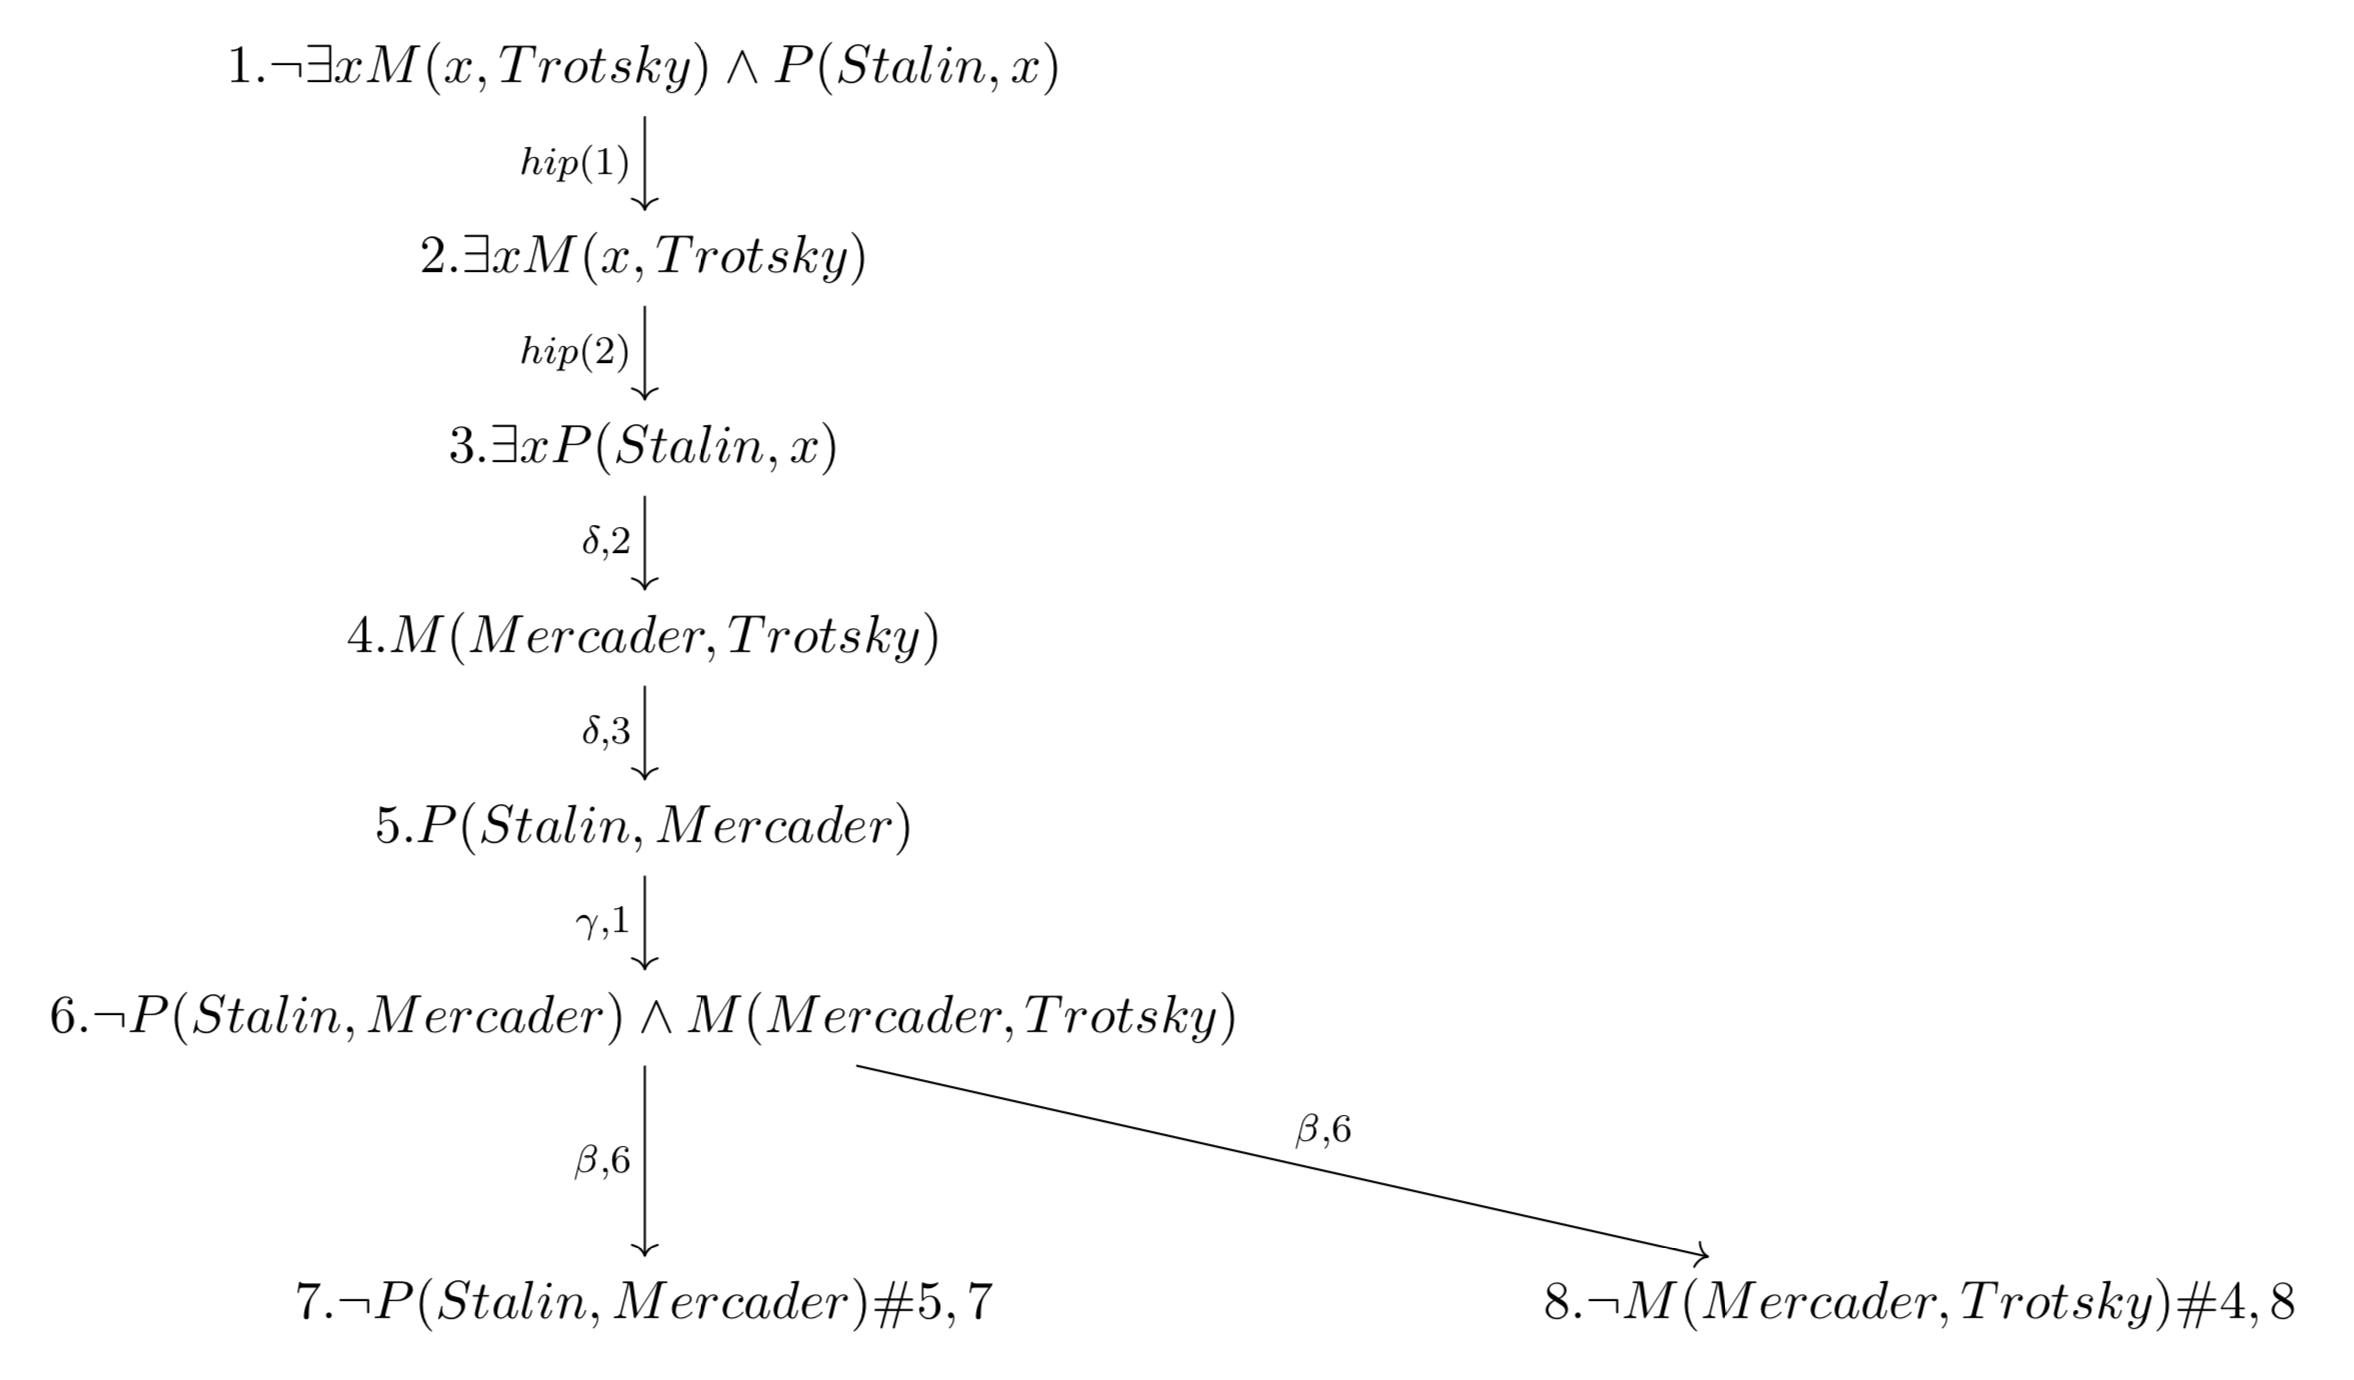
\includegraphics[scale = 0.36]{figures/tableau3.png}
\end{center}

En el punto 4 hemos aplicado correctamente una regla $\delta$ introduciendo la constante auxiliar $Mercader$, y en el 5 hemos vuelto a introducirla por la misma regla, es decir, hemos introducido una constante auxiliar no nueva en la rama. Esto nos ha llevado al absurdo de que la deducción original era válida.  
\end{example}

\begin{example}
Un ejemplo sencillo. Veamos si es válida la siguiente deducción:

\begin{center}
\syllog{Algunos niños son buenos} 
{Todo lo bueno se come} 
{Algunos niños se comen}
\end{center}
Que formalizamos como:
\begin{center}
\syllog{$\varphi_1$: $\exists x \, (ni(x)\land bu(x))$}
{$\varphi_2$: $\forall x \, (bu(x)\to co(x))$}
{$\psi$: $\exists x \, (ni(x)\land co(x))$}
\end{center}

Es decir, en este caso, $\Sigma = \{\varphi_1, \varphi_2, \neg \psi \}$. Veamos un tableau cerrado de $\Sigma$:

\begin{comment}
\begin{tikzcd}
1.\exists x (ni(x)\land bu(x)) \arrow[d]                                          &                                                                       \\
2.  \forall x (bu(x)\to co(x)) \arrow[d]                                          &                                                                       \\
3.  \neg\exists x (ni(x)\land co(x)) \arrow[d, "{\delta, 1}"']                    &                                                                       \\
4. ni(Pepe)\land bu(Pepe) \arrow[d, "{\alpha, 4}"']                               & \text{(Donde $Pepe\in C_A$)}                                         \\
5. ni(Pepe) \arrow[d]                                                             &                                                                       \\
6. bu(Pepe) \arrow[d, "{\gamma,2,pepe/x}"]                                        &                                                                       \\
7.bu(Pepe)\to co(Pepe) \arrow[rd, "{\beta,7}"] \arrow[d, "{\beta,7}"]             &  \\
9.co(Pepe) \arrow[d, "{\gamma,3,pepe/x}"]                                         & {\neg bu(Pepe)\#6,8}                                                  \\
10.\neg(ni(pepe)\land co(Pepe)) \arrow[d, "{\beta, 10}"] \arrow[rd, "{\beta, 10}"] &                                                                       \\
{12.\neg co(Pepe)\#9,12}                                                          & {11.\neg ni(Pepe)\#5,11}                                             
\end{tikzcd}
\end{comment}

\begin{center}
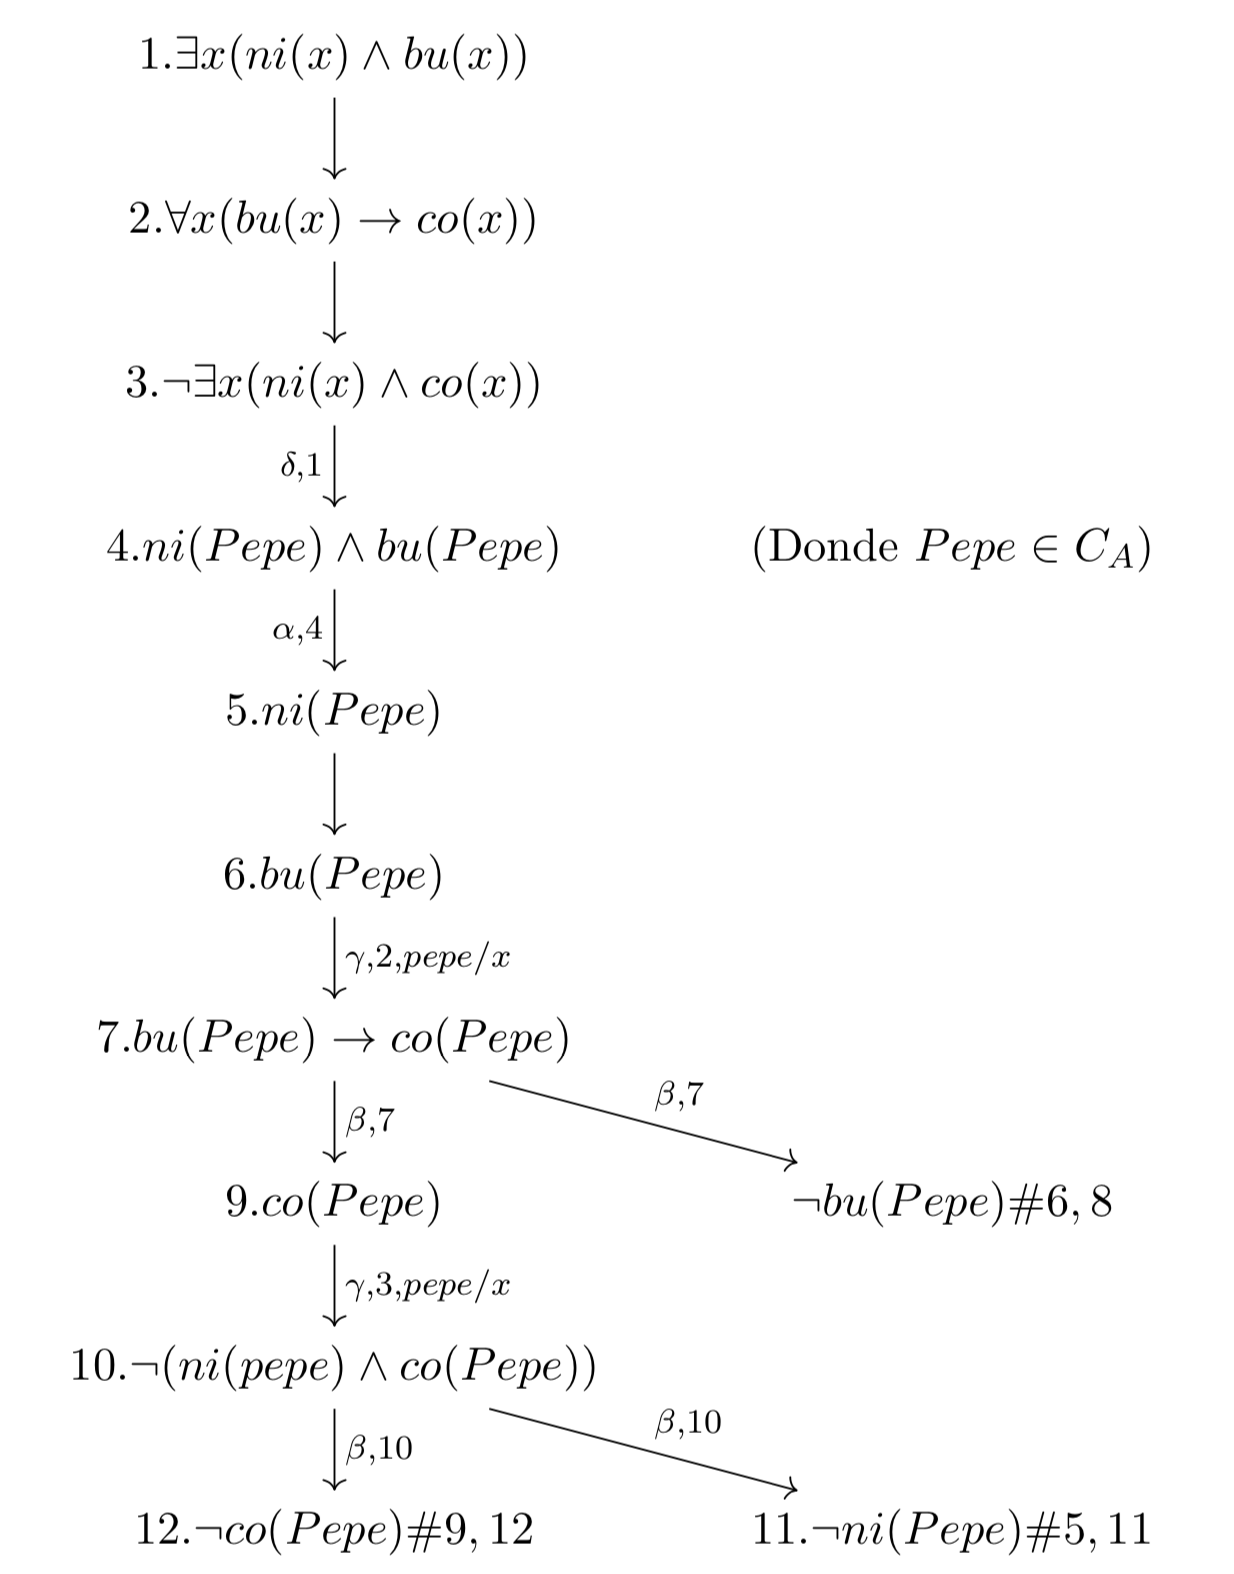
\includegraphics[scale = 0.44]{figures/tableau4.png}
\end{center}
\end{example}


\subsection{Corrección}

Tal y como hicimos en el método de los \textit{tableaux} para lógica proposicional, dados $\Phi \subseteq FORM_S$ y $\varphi \in FORM_S$, escribimos $\Phi \vdash_{tb} \varphi$ cuando existe un \textit{tableau} cerrado para $\Phi \cup \{\neg \varphi\}$.

Recordemos del capítulo anterior que decimos del método de los \textit{tableaux} que tiene \textit{corrección} si $\Phi \vdash_{tb} \varphi$ implica $\Phi \vDash \varphi$, y decimos que tiene \textit{completitud} si $\Phi \vDash \varphi$ implica $\Phi \vdash_{tb} \varphi$.\\
Vamos a comprobar que el método de los \textit{tableaux} de primer orden tiene ambas propiedades, empezando por la corrección.

Comencemos con el siguiente:

\begin{lema}\label{eq}
Para todo $\theta \in EQ_S$, $\vDash \theta$. 
\end{lema}
\begin{proof} \mbox{}
\begin{itemize}
        \item[(RF)] $\forall x \, x \doteq x$ es tautología ya que dada una interpretación $\mathfrak{I}$, se cumple $\mathfrak{I}[a/x] \vDash x \doteq x$ para todo $a \in A$, ya que obviamente $a=a$.
        \item[(IM)] $\forall x \, \forall y \, x \doteq y \rightarrow y \doteq x$ es tautología ya que, dada una interpretación $\mathfrak{I}$, se cumple $\mathfrak{I}[a/x][b/y] \vDash x \doteq y \rightarrow y \doteq x$ para todos $a,b \in A$, ya que si $a=b$, $\mathfrak{I}[a/x][b/y]$ verifica $x \doteq y$ y $y \doteq x$, por tanto verifica $x \doteq y \rightarrow y \doteq x$. Si $a\neq b$, $\mathfrak{I}[a/x][b/y]$ no verifican $x \doteq y$ ni $y \doteq x$, por tanto de nuevo verifica $x \doteq y \rightarrow y \doteq x$.
        \item[(TR)] $\forall x \, \forall t \, \forall z \, x \doteq y \land y \doteq z \rightarrow x \doteq z$ es una tautología. Este caso se demuestra de forma similar a los anteriores, comprobando que $\mathfrak{I}[a/x][b/y][c/z]$ siempre verifica $x \doteq y \land y \doteq z \rightarrow x \doteq z$. Se puede hacer como el apartado anterior dividiendo en los casos $a\neq b$, $a=b\neq c$, $a=b=c$.
        \item[(ST_{1})] Sea $f|_n \in Fn_S$. Entonces, $$\forall x_1, \dots, \forall x_n \, \forall y_1, \dots, \forall y_n \, \bigwedge\limits_{i = 1}^{n} x_i \doteq y_i \rightarrow f(x_1, \dots, x_n) \doteq f(y_1, \dots, y_n)$$ es una tautología. Se omite la demostración.
        \begin{comment}
        Este caso se demuestra por inducción en $n$.
        \begin{itemize}
            \item Caso base: Para cualquier constante (función 0-aria) $a$, cualquier interpretación verifica $a\doteq a$.
            \item Caso inductivo: Supongamos que cualquier función $n-1$-aria lo cumple. Sea f una función $n$-aria y sea una interpretación $\mathfrak{I}$. Entonces, $\mathfrak{I}$ verifica la función que buscamos si y solo si para todo $a\in A$, $\mathfrak{I}[a/x_1]$ verifica $$\forall x_2, \dots, \forall x_n \, \forall y_2, \dots, \forall y_n \, \bigwedge\limits_{i = 1}^{n} x_i \doteq y_i \rightarrow f(x_1, \dots, x_n) \doteq f(y_1, \dots, y_n).$$
            Esta fórmula es equivalente a:
            $$\forall x_2, \dots, \forall x_n \, \forall y_2, \dots, \forall y_n \, \neg (x_1\doteq y_1)\lor(\bigvee\limits_{i = 1}^{n} \neg (x_i \doteq y_i)) \lor f(x_1, \dots, x_n) \doteq f(y_1, \dots, y_n).$$
            Como ninguna variable aparece libre, por la ley (9) de equivalencia lógica esto equivale a:
            $$\neg (x_1\doteq y_1)\lor\forall x_2, \dots, \forall x_n \, \forall y_2, \dots, \forall y_n \, (\bigvee\limits_{i = 1}^{n} \neg (x_i \doteq y_i)) \lor f(x_1, \dots, x_n) \doteq f(y_1, \dots, y_n).$$
        \end{itemize}
        \end{comment}
        \item[(ST_{2})] Sea $p|_n \in Pd_S$. Entonces, $$\forall x_1, \dots, \forall x_n \, \forall y_1, \dots, \forall y_n \, \bigwedge\limits_{i = 1}^{n} x_i \doteq y_i \to  p(x_1, \dots, x_n) \rightarrow p(y_1, \dots, y_n)$$ es una tautología. Se omite la demostración.
\end{itemize}
\end{proof}

El siguiente resultado es fundamental, nos permite extender una rama satisfactible del \textit{tableaux} a otra que también lo es:

\begin{prop}\label{aaa}
Sea $S$ signatura. Sean $\Phi \subseteq FORM_S$ y $\mathfrak{I}$ $S$-interpretación tales que $\mathfrak{I} \vDash \Phi$. Entonces existe una $S$-interpretación $\mathfrak{I}'$ tal que $\mathfrak{I} \sim_{\varphi} \mathfrak{I}'$ para toda $\varphi \in \Phi$ de modo que:
\begin{enumerate}
    \item Sea $\sigma \in \Phi$ fórmula simplificable. Entonces $\mathfrak{I}' \vDash \Phi \cup \{\sigma_1 \}$, con $\sigma \sim \sigma_1$ la simplificación de $\sigma$.
    \item Sea $\alpha \in \Phi$ una $\alpha$-fórmula. Entonces $\mathfrak{I}' \vDash \Phi \cup \{\alpha_1, \alpha_2 \}$, con $\alpha \sim \alpha_1 \land \alpha_2$ la descomposición de $\alpha$.
    \item Sea $\beta \in \Phi$ una $\beta$-fórmula. Entonces $\mathfrak{I}' \vDash \Phi \cup \{\beta_1\}$ o $\mathfrak{I}' \vDash \Phi \cup \{\beta_2\}$, con $\beta \sim \beta_1 \lor \beta_2$ la descomposición de $\beta$.
    \item Sean $\gamma \in \Phi$ $\gamma$-fórmula, $t \in TERM_S$. Entonces $\mathfrak{I}' \vDash \Phi \cup \{\gamma(t)\}$.
    \item Sean $\delta \in \Phi$ $\delta$-fórmula, $c \in C_A$ constante auxiliar nueva en $\Phi$. Entonces $\mathfrak{I}' \vDash \Phi \cup \{\delta(c)\}$.
    \item Para cada $\theta \in EQ_S$, $\mathfrak{I}' \vDash \Phi \cup \{ \theta\}$.
\end{enumerate}
\end{prop}
\begin{proof} \mbox{}

(1), (2) y (3) son análogos a los de lógica proposicional. Basta hacer que $\mathfrak{I} = \mathfrak{I}'$ y el hecho de que:$$\sigma \sim \sigma_1, \quad \alpha \sim \alpha_1 \land \alpha_2, \quad \beta \sim \beta_1 \lor \beta_2.$$ \\

Veamos (4). Sea $\gamma \in \Phi$ y supongamos, sin pérdida de generalidad, que $\gamma$ es de la forma $\forall x \, \varphi$ (si fuese de la forma $\neg \exists x \, \varphi$, usamos que esto es equivalente a $\forall x \, \neg \varphi$ y hacemos $\psi := \neg \varphi$). Tomemos $\mathfrak{I}' = \mathfrak{I}$.

\noindent Consideremos el conjunto soporte de la interpretación $\mathfrak{I}$, $A$. Sea $t \in TERM_S$, y sea $a := t^{\mathfrak{I}} \in A$. Dado que $\forall x \, \varphi \in \Phi$, por hipótesis, $\mathfrak{I} \vDash \forall x \, \varphi$, y por tanto, $\mathfrak{I}[b/x] \vDash \varphi$ para todo $b \in A$, en especial, $\mathfrak{I}[a/x] \vDash \varphi$. Por el Lema de Sustitución, $\mathfrak{I} \vDash \varphi[t/x]$, y notando que $\varphi[t/x] = \gamma(t)$, obtenemos el resultado. \\

Veamos (5). Sea $\delta \in \Phi$ y supongamos que $\delta = \exists x \, \varphi$, para $\varphi \in FORM_S$ (en caso de que $\delta$ fuese de la forma $\neg \forall x \, \varphi$, entonces sería equivalente a $\exists x \, \neg \varphi$ y, haciendo que $\psi := \neg \varphi$, habríamos terminado). Sea $c \in C_A$ constante auxiliar nueva en $\Phi$.

\noindent Consideremos de nuevo el conjunto soporte de $\mathfrak{I} := \langle \mathfrak{A}, \sigma \rangle$, $A$. Como $\exists x \, \varphi \in \Phi$, por hipótesis, $\mathfrak{I} \vDash \exists x \, \varphi$, luego existe $a \in A$ tal que $\mathfrak{I}[a/x] \vDash \varphi$. Ahora definimos $\mathfrak{A}'$ como $\mathfrak{A}$ excepto que $c^{\mathfrak{A}'} = a$. Definamos $\mathfrak{I}' := \langle \mathfrak{A}', \sigma \rangle$. 

\noindent Al ser $c$ constante nueva para $\Phi$, es decir, para cada elemento de $\Phi$, tenemos que $\mathfrak{I} \sim_{\psi} \mathfrak{I}'$, para cada $\psi \in \Phi$, por tanto se cumple $\mathfrak{I} \vDash \psi$ para toda $\psi\in\Phi$. Por el Lema de Sustitución, 
$$(\varphi[c/x])^{\mathfrak{I}'} = \varphi^{\mathfrak{I}'[c^{\mathfrak{I}'}/x]} = \varphi^{\mathfrak{I}'[a/x]}.$$
Y dado que $\mathfrak{I}'[a/x] \sim_{\varphi} \mathfrak{I}[a/x]$ por ser $c$ nueva, aplicando una vez más el Lema de Sustitución, 
$$\varphi^{\mathfrak{I}'[a/x]} = \varphi^{\mathfrak{I}[a/x]} = V.$$
Lo que nos da el resultado. \\

Finalmente, (6) se deduce de \ref{eq}. 
\end{proof}

Del siguiente resultado se deducirá como corolario la corrección del método de los \textit{tableaux} de primer orden:

\begin{theorem}\label{bbb}
Sea $S$ signatura. Sea $\Phi \subseteq FORM_S$ conjunto de fórmulas satisfactible y $T$ un tableau finito para $\Phi$. Entonces $T$ es abierto y existe una rama abierta de $T$, $r$, tal que $\Gamma_r$ es satisfactible.
\end{theorem}
\begin{proof}
Demostremos que existe una $S$-interpretación $\mathfrak{I}$ y una tal rama $r$ de modo que $\mathfrak{I} \vDash \Phi$ y $\mathfrak{I} \vDash \Gamma_r$. 

Al ser $T$ finito, se ha construido en un número finito de reglas $R_{ini}, R_1,  \dots, R_{n}$, dando lugar la sucesión de \textit{tableaux} $T_0, T_1, \dots, T_n = T$. Por tanto, procedemos por inducción sobre $n$. \\

Si $n=0$, entonces $T_0$ es un \textit{tableau} inicial, es decir, tiene la forma 
\begin{tikzcd}
\varphi_1 \arrow[d, no head]          \\
\varphi_2 \arrow[dd, no head, dotted] \\ 
                                      \\
\varphi_k                            
\end{tikzcd}.
Entonces $r$ es la única rama disponible, y $\Gamma_r = \{ \varphi_1, \dots, \varphi_k\} \subseteq \Phi$, por lo que, dado que $\Phi$ es satisfactible, $\Gamma_r$ lo es. Por tanto, hemos encontrado una $S$-interpretación que verifica lo deseado. \\

Sea $n>0$ y supongamos que el resultado es cierto para el \textit{tableau} $T_{n-1}$ y veamos que lo es para $T_n$. Al aplicar la regla $R_n$ a $T_{n-1}$, extendemos una rama $r$. Además, por hipótesis de inducción, hay una rama $r'$ tal que $\Gamma_{r'}$ es satisfactible. \\

Si $r \neq r'$ entonces $r'$ es rama de $T_n$ y, como hemos dicho, verifica que $\Gamma_{r'}$ es satisfactible, con lo que obtenemos el resultado. \\

Si $r = r'$, debemos distinguir los siguientes casos, dependiendo de qué tipo de regla es $R_n$:
\begin{enumerate}
    \item $R_n$ es una regla inicial, de tipo $\sigma$, $\alpha$ o $\beta$. La demostración es análoga a la que vimos en lógica proposicional.
    \item $R_n$ es una regla $\delta$. Sea $\Gamma_{r}^{k}$ el conjunto de fórmulas de la rama $r$ en el árbol $k$-ésimo. Entonces existe $\delta \in \Gamma_{r}^{n-1}$ tal que $\Gamma_{r}^{n} = \Gamma_{r}^{n-1} \cup \{\delta(c)\}$, con $c \in C_A$ nueva en $r$. Por hipótesis de inducción, existe una $S$-interpretación $\mathfrak{I}$ tal que $\mathfrak{I} \vDash \Phi$ y $\mathfrak{I} \vDash \Gamma_{r}^{n-1}$.
    
    Por \ref{aaa}, existe $\mathfrak{I}'$ tal que $\mathfrak{I}' \vDash \Gamma_{r}^{n-1} \cup \{\delta(c)\}$, es decir, tal que $\mathfrak{I}' \vDash \Gamma_{r}^{n}$. Al ser $c$ nueva en $r$, $c \notin voc(\psi)$, para cada $\psi \in \Phi$, por tanto como en la prueba de \ref{aaa} vimos que $\mathfrak{I}'$ solo difiere de $\mathfrak{I}$ en $c$, $\mathfrak{I}' \sim_{\psi} \mathfrak{I}$, y por tanto $\mathfrak{I}' \vDash \psi$, es decir, $\mathfrak{I}' \vDash \Phi$.
    
    \item $R_n$ es una regla $\gamma$. Existe $\gamma \in \Gamma_{r}^{n-1}$ tal que $\Gamma_{r}^{n} = \Gamma_{r}^{n-1} \cup \{\gamma(t)\}$, siendo $t \in TERM_S$. Por hipótesis, existe una $S$-interpretación $\mathfrak{I}$ con $\mathfrak{I} \vDash \Phi$ y $\mathfrak{I} \vDash \Gamma_{r}^{n-1}$. 
    
    Por la prueba de \ref{aaa}, la misma $\mathfrak{I}$ cumple $\mathfrak{I} \vDash \Gamma_{r}^{n-1} \cup \{\gamma(t)\}$, por tanto $\mathfrak{I} \vDash \Gamma_{r}^n$.
    
    \item $R_n$ es una regla $\theta$, con $\theta \in EQ_S$. Entonces, $\Gamma_{r}^{n} = \Gamma_{r}^{n-1} \cup \{\theta\}$. Por hipótesis de inducción, existe una $S$-interpretación $\mathfrak{I}$ tal que $\mathfrak{I} \vDash \Phi$ y, $\mathfrak{I} \vDash \Gamma_{r}^{n-1}$. Por tanto, $\mathfrak{I} \vDash \Gamma_{r}^n$.
\end{enumerate}
\end{proof}

\begin{cor}\label{ccc}
Sea $S$ signatura. Si $\Phi \subseteq FORM_S$ y $\Phi$ tiene un \textit{tableau} cerrado, entonces $\Phi$ es insatisfactible. 
\end{cor}
\begin{proof}
Basta notar que este enunciado es la forma contrapositiva de \ref{bbb}.
\end{proof}

Finalmente, obtenemos el resultado al que hemos dedicado esta subsección:

\begin{cor}(Corrección)
Sean $S$ signatura, $\Phi \subseteq FORM_S$, $\varphi \in FORM_S$. Entonces, si $\Phi \vdash_{tb} \varphi$, entonces $\Phi \vDash \varphi$.
\end{cor}
\begin{proof}
Si $\Phi \vdash_{tb} \varphi$, entonces $\Phi \cup \{\neg \varphi \}$ tiene un \textit{tableau} cerrado y, por \ref{ccc}, $\Phi \cup \{\neg \varphi \}$ es insatisfactible. Por el resultado análogo a \ref{\text{Insat}} para lógica de primer orden, esto implica que $\Phi \vDash \varphi$.
\end{proof}


\subsection{Completitud. Conceptos Básicos}

El estudio de la completitud va a ser más complicado que en lógica proposicional. Para poder estudiarla, vamos a necesitar introducir una serie de nociones fundamentales de teoría de grafos: 

\begin{defs}\mbox{}
\begin{enumerate}[label=\bold{\arabic*})]
    \item Un \textit{grafo no dirigido} es un par ordenado $T = \langle N, E \rangle$, donde $N$ es el conjunto de \textit{nodos} y $E$ es el conjunto de \textit{aristas}, que son pares sin ordenar de nodos distintos.
    \item Un camino es una sucesión de $(\geq1)$ aristas $(a_1,\dots,a_n)$ de forma que  $a_i$ comparte uno de sus vértices con $a_{i-1}$ y el otro con $a_{i+1}$ para $i=2,3,\dots,n-1$. Llamamos a $n$ \textit{longitud del camino}.
    \item Decimos que el camino es \textit{simple} si cada vértice del camino solo aparece hasta dos veces, una al final de una arista y otra al principio de la siguiente. Decimos que un camino es un \textit{ciclo} si es simple y el primer vértice de la primera arista es el segundo vértice de la última arista.
    \item Decimos que un grafo es \textit{acíclico} si no tiene ciclos. Decimos que un grafo es \textit{conexo} si para cada par de nodos hay un camino entre ellos.
    \item Un \textit{árbol (libre)} es un grafo no dirigido conexo y acíclico. Equivalentemente, es un grafo tal que entre cada par de sus nodos hay un solo camino simple que los une.
    \item Sea $G = \langle V, E\rangle$ grafo no dirigido. Se llama \textit{grado} de $v \in V$, $deg(v)$, al número de elementos de $E$ que inciden sobre él.
\end{enumerate}
\end{defs}


Se tienen las siguientes propiedades:

\begin{prop}
Sea $T = \langle N, E \rangle$ un grafo:
\begin{enumerate}
    \item Si $T$ es un árbol y le quitamos un elemento de $E$, $T$ deja de ser conexo.
    \item Si $T$ tiene finitos nodos, $T$ es un árbol si y solo si $|E| = |N| - 1$.
\end{enumerate}
\end{prop}
\begin{proof}
Se omite la demostración.
\end{proof}

\begin{defs}\mbox{}
\begin{enumerate}[label=\bold{\arabic*})]
    \item Un árbol $T = \langle N, E \rangle$ se llama \textit{árbol con raíz} si se selecciona un elemento especial de $N$, llamado \textit{raíz} de $T$.
    \item Sea $T = \langle N, E \rangle$ árbol con raíz $n_0$. Se llama \textit{altura} de $n \in N$, $h(n)$, a la longitud del único camino simple que une $n_0$ con $n$.
    \item Sea $T = \langle N, E \rangle$ árbol de raíz $n_0$. Se dice que $n_1\in N$ es \textit{hijo de} $n$ si hay una arista que conecta $n$ y $n_1$ y $h(n_1)=h(n)+1$. Se dice que $n_1$ y $n_2$ son \textit{hermanos} si son hijos del mismo nodo.
    \item Sea $T = \langle N, E \rangle$ árbol de raíz $n_0$. Llamamos \textit{rama finita} a un camino simple desde $n_0$ que no está contenido en ningún otro camino simple desde $n_0$. Una \textit{rama infinita} será una sucesión de aristas $a_1,a_2,\dots$ tal que $a_i$ comparte un vértice con $a_{i-1}$ y el otro con $a_{i+1}$ para $i\geq2$, que parte desde $n_0$ y en que no se repiten vértices (es decir, como un camino simple desde $n_0$ pero con infinitos vértices).
\end{enumerate}
\end{defs}

De ahora en adelante consideraremos árboles con una raíz determinada.

\begin{definition}
Sean $T_1 := \langle N_1, E_1 \rangle$, $T_2 :=  \langle N_2, E_2 \rangle$ dos árboles con la misma raíz. Decimos que $T_1$ \textit{está incluido en} $T_2$, $T_1 \leq T_2$, si:
\begin{itemize}
    \item $N_1 \subseteq N_2$.
    \item $E_1 \subseteq E_2$.
\end{itemize}
\end{definition}

\begin{definition}
Sean $T_0, \dots, T_k, \dots$ árboles tales que $T_0 \leq \dots \leq T_k \leq \dots$. Definimos:
$$\lim_{n \in \mathbb{N}} T_n := \langle N, E \rangle$$
siendo $N := \bigcup_{n\in \mathbb{N}} N_{n}$ y $E := \bigcup_{n\in \mathbb{N}} E_{n}$ y con la misma raíz que la de T_0.
\end{definition}

\begin{prop}
Sea $T_0 \leq \dots \leq T_k \leq \dots$ sucesión de árboles. Sea $T := \lim_{n \in \mathbb{N}} T_n$. Entonces:
\begin{enumerate}
    \item $T_i \leq T$, para todo $i \in \mathbb{N}$.
    \item $T$ es un árbol.
\end{enumerate}
\end{prop}
\begin{proof}\mbox{}
\begin{enumerate}
    \item Se sigue de las definiciones anteriores.
    \item Comencemos demostrando que $T = \langle T, N\rangle$ es conexo. Sean $n_1, n_2 \in N$. Como $N := \bigcup_{n\in \mathbb{N}} N_{n}$ y $N_i \subseteq N_j$, para todo $i \leq j$, existe $k \in \mathbb{N}$ tal que $n_1, n_2 \in N_k$. Al ser $T_k = \langle N_k, E_k\rangle$ conexo, existe un camino en $T_k$ que une $n_1$ y $n_2$. Al ser $E_k \subseteq E$ por definición, también es un camino en $T$, lo que nos da la conexión de $T$. \\
    
    Supongamos que existen dos nodos $n_1, n_2 \in N$ tales que existen dos caminos simples distintos $e_1, \dots, e_l$ y $f_1, \dots, f_k$ que los conectan. Es claro, razonando igual que antes, que existe $i \in \mathbb{N}$ tal que $n_1, n_2 \in N_i$ y $e_1, \dots, e_l, f_1, \dots, f_k \in E_i$ y, al ser $T_i = \langle N_i, E_i\rangle$ árbol, $e_1, \dots, e_l$ y $f_1, \dots, f_k$ son iguales, lo que implica que $T$ sea acíclico.
\end{enumerate}
\end{proof}

Nótese que nuestros \textit{tableaux} son árboles con raíz. Además, se cumplirá que las ramas cerradas serán siempre finitas, ya que una rama cerrada se forma cuando dos fórmulas en la rama están en contradicción y ya no hace falta seguir extendiendo la rama.


Necesitamos el siguiente resultado técnico de la teoría de grafos:

\begin{theorem}(Lema de König para árboles)\label{konig}
\mbox{}
Sea $T$ un árbol con raíz con infinitos nodos tal que cada nodo tiene finitos hijos. Entonces $T$ tiene una rama infinita.
\end{theorem}
\begin{proof}
\begin{comment}
Supongamos que tenemos una ordenación de los vértices, $(v_n)_{n\in\mathbb{N}}$. La raíz del árbol será $v_{i_0}$. Dados dos nodos $a$ y $b$ distintos, decimos que $b$ es descendiente de $a$ si el único camino simple $c_b$ desde $v_0$ hasta $b$ pasa por $a$. Como $b\neq a$, en $c_b$ tenemos un vértice siguiente a $a$, que por tanto es hijo de $a$. De modo que cualquier descendiente de un vértice es uno de sus hijos o descendiente de uno de sus hijos.\\[-7pt]

Entonces, $v_{i_0}$ tiene infinitos descendientes (todos los vértices salvo $v_0$). Estos infinitos descendientes contienen a los finitos hijos de $v_{i_0}$ y a sus descendientes. Por tanto alguno de sus hijos tiene que tener infinitos descendientes. Sea $v_{i_1}$ el menor de ellos. Como $v_{i_1}$ tiene infinitos descendientes, de la misma forma que antes escogemos el menor de sus hijos, $v_{i_2}$, que tiene infinitos descendientes.\\[-7pt]

De este modo creamos una sucesión de vértices $(v_{i_n})_{n\in\mathbb{N}}$. Como por definición $v_{i_n}$ tiene altura $n$, no se repiten vértices. Por tanto la sucesión de aristas $a_n$ que unen $v_{i_n}$ con $v_{i_{n+1}}$ forman una rama infinita.
\end{comment}
\end{proof}


\begin{comment}
\begin{theorem}(Lema de König)\label{konig}
Sea $G$ grafo que verifica lo siguiente:
\begin{enumerate}
    \item $G$ es conexo.
    \item $G$ es \textit{localmente finito}, es decir, cada nodo es vecino de finitos vértices.
    \item $G$ es \textit{infinito}, es decir, su conjunto de nodos es infinito.
\end{enumerate}
Entonces $G$ contiene un camino simple infinito.

En especial, cada árbol infinito contiene o un nodo de grado infinito o un camino simple infinito.
\end{theorem}
\begin{proof}
Se omite la demostración.
\end{proof}
\end{comment}


\begin{prop} \label{cefi}
Si $T$ es tableau cerrado, es finito.
\end{prop}
\begin{comment}
\begin{proof}
Observemos que, en todo \textit{tableau}, el número máximo de hijos de cada nodo es dos: los que se pueden obtener por la aplicación de una regla $\beta$.
Al ser $T$ cerrado, en cada rama suya $r$ hay dos nodos $n_1, n_2$ que son contradictorios. Definimos:
$$h_r := max\{h(n_1), h(n_2)\}$$
$$h := max\{h_r \, | \, r \text{ rama de } T\}$$

Si $h$ fuese infinito, el árbol tendría ramas $r$ con $h_r$ arbitraria. Como cada nodo tiene a lo sumo dos hijos, por \ref{konig} debe tener una camino simple infinito, esto es, una rama infinita. Esta rama infinita no puede estar cerrada, ya que las ramas cerradas tienen siempre profundidad finita.

Por tanto, $h$ es finito y, del hecho de que cada nodo tiene a lo sumo dos hijos deducimos que tiene que ser finito.
\end{proof}
\end{comment}
\begin{proof}
Usaremos reducción al absurdo. Sea $T$ un \textit{tableaux} infinito cerrado. Observemos que, en todo \textit{tableau}, el número máximo de hijos de cada nodo es dos: los que se pueden obtener por la aplicación de una regla $\beta$. Por tanto, por el lema de König $\ref{konig}$ el \textit{tableau} contiene una rama infinita. Esto contradice el hecho de que todas las ramas cerradas son finitas.
\end{proof}

\subsection{Conjuntos de Hintikka para lógica de primer orden}\label{Hinti33}

Para continuar con el teorema de completitud, lo siguiente es definir
el análogo a los conjuntos de Hintikka que vimos en la lógica
proposicional, pero ahora para la lógica de primer orden.

Lo primero que necesitamos es el concepto de \emph{término adecuado}
para un conjunto de fórmulas $\Phi\subseteq FORM_S$


\begin{definition}
  Sea S una signatura, $t\in TERM_S$ y $\Phi\subseteq FORM_S$. Diremos que
  $t$ es \emph{adecuado} para $\Phi$ si se cumple:
  \begin{itemize}
  \item $voc(t)\subseteq voc(\Phi):=\bigcup\limits_{\varphi\in\Phi} voc(\varphi)$
  \item $var(t)\subseteq lib(\Phi):=\bigcup\limits_{\varphi\in\Phi} lib(\varphi)$
  \end{itemize}
\end{definition}
\\ \\
\noindent Puede darse el caso de que no encontremos ningún término adecuado para un conjunto de fórmulas. Por ejemplo consideremos el conjunto de fórmulas
\begin{displaymath}
  \Phi = \{\exists x\ (p(x)\to q(x))\}
\end{displaymath}
En este caso
$(voc(\Phi)\cap\mathit{Ct}_{S})\cup lib(\Phi)=\emptyset$, por tanto no podemos construir términos adecuados. En este caso, como en el método de los \textit{tableaux} nos serán necesarios términos adecuados para desarrollar el algoritmo, tomaremos como término adecuado cualquier constante auxiliar $c\in C_A$ nueva.

\begin{definition}[Conjunto de Hintikka]
  Sea $S$ una signatura,  $\Phi\in FORM_S$ y $T_{\Phi}:=\{t\ |\ t\in TERM_S\
  \mbox{adecuado para}\ \Phi\}$. Diremos que \(\Phi\) es de
  \emph{Hintikka}
  si verifica todas estas propiedades:
  \begin{itemize}
  \item \(\Phi\) es coherente:
    \begin{itemize}
    \item $\bot\not\in\Phi$
    \item no existe $\varphi\in\Phi$ tal que \(\neg\varphi\in\Phi\).
    \end{itemize}
  \item \(\Phi\) es \(\alpha\)-saturado: si \(\alpha\in\Phi\) es una
    \(\alpha\)-fórmula, \(\alpha_{1},\alpha_{2}\in\Phi\).
  \item \(\Phi\) es \(\beta\)-saturado: si \(\beta\in\Phi\) es una
    \(\beta\)-fórmula, \(\beta_{1}\in \Phi\) o \(\beta_{2}\in\Phi\).
  \item \(\Phi\) es \(\sigma\)-saturado: si \(\sigma\in\Phi\) es una
    \(\sigma\)-fórmula, \(\sigma_1\in \Phi\).
  \item \(\Phi\) es \(\gamma\)-saturado: si \(\gamma\in\Phi\) es una
    \(\gamma\)-fórmula y \(t\in T_{\Phi}\), entonces \(\gamma(t)\in \Phi\).
  \item \(\Phi\) es \(\delta\)-saturado: si \(\delta\in\Phi\) es una
    \(\delta\)-fórmula, entonces existe una constante auxiliar
    $c\in C_{A}$ tal que \(\delta(c)\in \Phi\).
  \item \(\Phi\) es \(\theta\)-saturado: si
    \(\theta\in\mathrm{EQ}_{S}\) es un axioma de igualdad, entonces
    \(\theta\in\Phi\).
  \end{itemize}
\end{definition}
 \\ \\ \\

Consideremos a continuación una signatura cualquiera $S$. Nuestra intención es demostrar que todo conjunto $\Phi\subseteq FORM_S$ de Hintikka es satisfactible. Es decir, tenemos que crear una interpretación, con una álgebra $\mathfrak{T}$ y una asignación de  variables $\sigma_\Phi$, que haga ciertas todas las fórmulas de $\Phi$. El primer paso  para ello  es encontrar un conjunto soporte para nuestra álgebra. \\
Una opción a considerar es el \textit{álgebra libre de términos}, una álgebra conocida que tiene como como conjunto soporte a $TERM_S$. Sin embargo, esta álgebra no es suficiente: Supongamos que tenemos la signatura de
la aritmética. Según esta signatura, los términos
\(s(0)+0\) y \(s(0)\) son distintos, pero representan el mismo elemento. Eso se traduce en que en nuesto álgebra necesitamos establecer una relación de
equivalencia de términos. Esa relación la denotaremos como
$\equiv_{\Phi}$, la idea es que $t\equiv_{\Phi} s$ si $\Phi\models
t\doteq s$.


\begin{definition}
  Dada $S$ una signatura, $\Phi\subseteq FORM_S$ y
  $s,t\in TERM_S$ definimos la equivalencia de términos como:
  
   $$ t\equiv_{\Phi}s\quad\text{si y solo si}\quad t\doteq s\in\Phi $$
 
\end{definition}
 
 
\begin{prop}
  Sea $S$ signatura, \(\Phi\subseteq FORM_S\). Si $\Phi$ es de Hintikka, entonces \(\equiv_{\Phi}\subseteq
  T_{\Phi}\times T_{\Phi}\) es relación de equivalencia.

\begin{proof} Probamos las propiedades reflexiva, simétrica y transitiva.
    \begin{enumerate}
        \item \textit{Propiedad reflexiva.} Dado $t\in T_\Phi$ hay que probar que $t\equiv_{\Phi} t$. Utilizaremos el axioma de reflexión (RF), que está en $\Phi$ por ser de $Hintikka$.
        \[
            \gamma := (\forall x\ x\doteq x) \in \Phi
        \]
        Es una $\gamma$-fórmula, luego por ser $\Phi$ de $Hintikka$, $\gamma(t) \in \Phi$, esto es:
        \[
            t\doteq t\ \in \Phi
        \]
        lo que equivale a que $t\equiv_{\Phi} t$, que es el resultado deseado.
        \item \textit{Propiedad simétrica.} Sean $t,s\in T_{\Phi}$ tales que \(t\equiv_{\Phi} s\), es decir,
    \(t\doteq s\in\Phi\). Al ser $\Phi$ de Hintikka contiene al axioma de simetría (IM):
    \[
         \gamma\ :=\ (\forall x \, \forall y \, x \doteq y \rightarrow y \doteq x)
    \]
    que es una $\gamma$-fórmula, por lo que $\gamma(t) \in \Phi$:
    \[
        \gamma(t)\ =\ (\forall y \, t \doteq y \rightarrow y \doteq t)
    \]
    que es de nuevo otra $\gamma$-fórmula. Se aplica nuevamente la misma regla para $s$ y se tiene que:
    \[
        \gamma(t)(s)\ =\ (t \doteq s \rightarrow s \doteq t) \in \Phi
    \]
    que es una $\beta$-fórmula, luego se cumple:
    \[
        \neg t \doteq s \in \Phi\ \ o\ \ s \doteq t \in \Phi
    \]
    Como se sabe ya que $t \doteq s \in \Phi$ no queda otra que $s \doteq t \in \Phi$, que equivale a que $s\equiv_{\Phi} t$, como queríamos probar.
    \item \textit{Propiedad transitiva.} Dados $t,s,r\in T_{\Phi}$ tal que $t\equiv_{\Phi} s$ y  $s\equiv_{\Phi} r$, hay que desmostrar que $t\equiv_{\Phi} r$. El axioma de transitividad está en $\Phi$, luego:
    \[
        \gamma\ :=\ (\forall x\forall y \forall z\ x\doteq y \land y\doteq z \rightarrow x\doteq z) \in \Phi
    \]
    que es una $\gamma$-fórmula. Aplicando los cambios de las variables por los términos y atendiendo a que $\Phi$ es $\gamma$-saturado por ser de Hintikka se tiene:
    \[
        \gamma(t)(r)(s)\ =\ (t\doteq s \land s\doteq r \rightarrow t\doteq r) \in \Phi
    \] 
    que es una $\beta$-fórmula. Entonces:
    \[
        \neg(t\doteq s \land s\doteq r)\in \Phi\ \ o \ \ t\doteq r \in \Phi
    \]
    Veamos que la primera no se cumple: de ser así, y al ser una $\beta$-fórmula, se tendría que:
    \[
        \neg(t \doteq s)\in \Phi\ \ o\ \  \neg(s\doteq r)\in \Phi
    \]
    pero esto es imposible por la coherencia de $\Phi$, pues tanto $t \doteq s$ como $s\doteq r$ están en $\Phi$. Se deduce que necesariamente $t\doteq r \in \Phi$ y entonces $t\equiv_{\Phi} r$.
    \end{enumerate}
\end{proof}
\end{prop}

Dada una relación de equivalencia $\equiv_{\Phi}$ podemos crear de forma natural una partición del conjunto  considerando el conjunto cociente, es decir, el conjunto de clases de equivalencia inducido por $\equiv_{\Phi}$. Dado $t\in T_{\Phi}$, se tiene su clase de equivalencia:
\begin{displaymath}
  [t] := \{s\ |\ s\in T_{\Phi}, t\equiv_{\Phi}s\}
\end{displaymath}
y entonces el conjunto cociente es:
\begin{displaymath}
  T_{\Phi}/\equiv_{\Phi}\quad =\quad \{[t]\ |\ t\in T_{\Phi}\}
\end{displaymath}
El soporte del álgebra que vamos a construir es precisamente este conjunto cociente.

\noindent Ahora hay que definir el valor de las constantes,
las funciones y los símbolos de predicado en el conjunto cociente. 
\begin{itemize}
\item Si $c\in Ct_{S}$ definimos
  \begin{displaymath}
    c^{\mathfrak{T}_{\Phi}}=\left\{
      \begin{array}{ll}
        [c] & \mbox{si}\ c\in T_{\Phi}\\
        \mbox{arbitrario}\footnotemark & \mbox{si no}
      \end{array}
    \right.
  \end{displaymath}
  \footnotetext{Por el lema de coincidencia, para nuestros propósitos no importará el valor que
    tenga.}

\item Si $f|_{k}\in Fn_{S}$ y \(t_{1},\dots t_{k}\in T_{\Phi}\)
  \begin{displaymath}
    f^{\mathfrak{T}_{\Phi}}([t_{1}],\dots [t_{k}])=\left\{
      \begin{array}{ll}
        [f(t_{1},\dots t_{k})]& \mbox{si}\ f(t_{1},\dots t_{k})\in
                                 T_{\Phi}\\
        \mbox{arbitrario} & \mbox{si no}
      \end{array}
    \right.
  \end{displaymath}
\item Si $p|_{k}\in Pd_{S}$ y \(t_{1},\dots t_{k}\in T_{\Phi}\)
  \begin{displaymath}
    p^{\mathfrak{T}_{\Phi}}([t_{1}],\dots [t_{k}])=\left\{
      \begin{array}{ll}
        V & \mbox{si}\ p(t_{1},\dots t_{k})\in\Phi\\
        F & \mbox{si no}
      \end{array}
    \right.
  \end{displaymath}
\end{itemize}

Veamos a continuación que el valor de una clase está bien definido, es decir, no depende de los representantes escogidos:

\begin{prop}
  Sea $S$ una signatura, $\Phi\subseteq FORM_S$ un conjunto de fórmulas de
  Hintikka, $t_{1},\ldots t_{k},s_{1},\ldots,s_{k}\in T_{\Phi}$
  términos tales que $[t_{i}]=[s_{i}]$ para $1\leq i\leq k$.
  \begin{itemize}
  \item Si $f|_{k}\in voc(\Phi)$ entonces $[f(t_{1},\ldots t_{k})]=[f(s_{1},\ldots,s_{k})]$
  \item Si $p|_{k}\in voc(\Phi)$ entonces $p(t_{1},\ldots
    t_{k})\in\Phi$ si y solo si $p(s_{1},\ldots,s_{k})\in\Phi$
  \end{itemize}

  \begin{proof}
    En primer lugar veamos el caso de los símbolos de función.
    Puesto que
    \(\Phi\)
    es de Hintikka tenemos que el axioma de igualdad
    \begin{displaymath}
      \gamma_{0}=\forall x_{1}\dots\forall x_{k}\forall y_{1}\dots \forall
      y_{k}\
      x_{1}\doteq y_{1}\land\dots\land x_{k}\doteq y_{k}\to
      f(x_{1},\dots,x_{k})\doteq f(y_{1},\dots,y_{k})\in\Phi
    \end{displaymath}
  Definimos ahora las siguientes fórmulas, que estarán en $\Phi$ por ser $\Phi$ de Hintikka:
  \begin{displaymath}
    \begin{array}{l}
      \displaystyle\gamma_{1}=\gamma_{0}(t_{1}),\ \ \gamma_{2}=\gamma_{1}(t_{2}),\ \ 
      \dots\ \ \gamma_{k}=\gamma_{k-1}(t_{k})\\
      \gamma_{k+1}=\gamma_{k}(s_{1}),\  \gamma_{k+2}(s_{2}),\ 
      \displaystyle\dots\ \gamma_{2k}=\gamma_{2k-1}(s_{k})\\
      \gamma_{2k}\ =\ t_{1}\doteq s_{1}\land\dots\land t_{k}\doteq s_{k}\rightarrow
      f(t_{1},\dots, t_{k})\doteq f(s_{1},\dots, s_{k})
    \end{array}
  \end{displaymath}
  Resulta que \(\gamma_{2k}\) es una \(\beta\)-fórmula.
  Por tanto \(\neg(t_{1}\doteq s_{1}\y\dots t_{k}\doteq s_{k})
  \in\Phi\) o
  \(f(t_{1},\dots, t_{k})\doteq f(s_{1},\dots, s_{k})\in\Phi\).
  Hay 2 casos:
  \begin{itemize}
  \item
    \(\neg(t_{1}\doteq s_{1}\y\dots t_{k}\doteq s_{k})
    \in\Phi\). Esta es una \(\beta\)-fórmula.
    En este caso, aplicando la regla $\beta$ repetidamente llegamos a que alguna de las fórmulas $\neg (t_{i}\doteq
    s_{i})$ está en $\Phi$. Por otro lado,
    $[t_{i}]=[s_{i}]$ significa \(t_{i}\doteq s_{i}\in\Phi\). Esto  contradice que \(\Phi\) sea de Hintikka, al tener
    $\neg (t_{i}\doteq  s_{i}), t_{i}\doteq  s_{i}\in\Phi$, por tanto este caso no puede darse.
  \item \(f(t_{1},\dots, t_{k})\doteq f(s_{1},\dots,
    s_{k})\in\Phi\). Esta es la definición de
    \( f(t_{1},\dots, t_{k})\equiv_{\Phi} f(s_{1},\dots,
    s_{k}) \), por tanto \( [f(t_{1},\dots, t_{k})]=[f(s_{1},\dots,
    s_{k})] \).
  \end{itemize}

Pasamos ahora a los símbolos de predicado. Nos vale probar que si $p(t_{1},\ldots
    t_{k})\in\Phi$, entonces $p(s_{1},\ldots,s_{k})\in\Phi$. En efecto, la  implicación recíproca es consecuencia de la  implicación directa al intercambiar $t_1,\dots,t_k$ por $s_1,\dots,s_k$ respectivamente.

    Puesto que
    \(\Phi\)
    es de Hintikka contiene el axioma de igualdad
    \begin{displaymath}
      \gamma_{0}=\forall x_{1}\dots\forall x_{k}\forall y_{1}\dots \forall
      y_{k}\
      x_{1}\doteq y_{1}\land\dots\land x_{k}\doteq y_{k}\to(
      p(x_{1},\dots,x_{k})\to p(y_{1},\dots,y_{k})\in\Phi).
    \end{displaymath}
  De forma similar a la vista los símbolos de función, llegamos a que la siguiente fórmula está en $\Phi$:  
\[\gamma_{2k}\ =\ t_{1}\doteq s_{1}\land\dots\land t_{k}\doteq s_{k}\rightarrow
      (p(t_{1},\dots, t_{k})\to p(s_{1},\dots, s_{k}))\]
  Por tanto, \(\neg(t_{1}\doteq s_{1}\y\dots t_{k}\doteq s_{k})
  \in\Phi\) o
  \(p(t_{1},\dots, t_{k})\to p(s_{1},\dots, s_{k})\in\Phi\).
  Hay 2 casos. En el primer caso, igual que con los símbolos de función llegamos a  un absurdo.  En el segundo caso, tenemos que $p(t_{1},\dots, t_{k})\to p(s_{1},\dots,
    s_{k})\in\Phi$. Esto implica, que  o bien $\neg(p(t_{1},\dots, t_{k}))\in\Phi$ en cuyo caso $p(t_{1},\dots, t_{k})\notin\Phi$, o bien $p(s_{1},\dots,
    s_{k})\in\Phi$. En ambos casos se cumple la implicación que buscamos.
\end{proof}
\end{prop}

Ya podemos definir el álgebra que buscamos:
\begin{displaymath}
  \mathfrak{T}_\Phi \ :=\ \bigl\langle
  T_{\Phi}/\equiv_{\Phi},\{c^{\mathfrak{T}_{\Phi}}:=[c]\ |\ c\in Ct_{S}\},
  \{f^{\mathfrak{T}_{\Phi}}\ |\ f|_{k}\in Fn_{S}\},
  \{p^{\mathfrak{T}_{\Phi}}\ |\ p|_{k}\in Pd_{S}\}
  \bigr\rangle
\end{displaymath}

Además, consideremos la asignación de variables:
\begin{displaymath}
  \sigma_{\Phi} :=\left\{
    \begin{array}{ll}
      [x] & \mbox{si } x \in T_{\Phi}\\
      \mbox{arbitrario} & \mbox{si no}
    \end{array}
\end{displaymath}

Y tomamos la interpretación:
\begin{displaymath}
  \mathfrak{I}_{\Phi} := \langle \mathfrak{T}_{\Phi}, \sigma_{\Phi}\rangle
\end{displaymath}

Veamos que \(\mathfrak{I}_{\Phi}\models\Phi\). En primer
lugar tenemos la siguiente 
\begin{prop}\label{prop:terminos}
  Sea $S$ una signatura, $\Phi\subseteq FORM_S$ un conjunto de fórmulas de
  Hintikka y $t\in T_{\Phi}$. Entonces \(t^{\mathfrak{I}_{\Phi}}=[t]\).

  \begin{proof}
Se puede hacer por inducción sobre la longitud de los términos. Para longitud 1, es directo de la definición en constantes y variables. Supongamos que se cumple para palabras de longitud $\leq n$, siendo $n>1$.\\
Ahora, si $t$ es un término de longitud $n$, será de la forma $f(t_1,\dots,t_k)$, donde los $t_i$ tienen longitudes $<n$. Por tanto, por hipótesis de inducción, se cumple $t_i^{\mathfrak{I}_{\Phi}}=[t_i]$ para $i=1,\dots,k$, ya que $t_i\in T_{\Phi}$ para todo $i$. Por tanto:
\[t^{\mathfrak{I}_{\Phi}}=f^{\mathfrak{I}_{\Phi}}([t_1],\dots,[t_k])=[f(t_1,\dots,t_k)],\]
lo cual completa la inducción.
  \end{proof}
\end{prop}

Ahora tenemos que demostrar \(\mathfrak{I}_\Phi \models\varphi\) para cada
\(\varphi\in\Phi\). Para esto no basta con inducción estructural, sino que nos interesa extender la norma que vimos en lógica proposicional:

\begin{definition}
  Sea $S$ una signatura. Definimos la \textit{norma} de una fórmula como:
  $$\|\cdot\|:FORM_S \rightarrow \N$$ de forma recursiva como sigue:
  \begin{itemize}
  \item Caso base: \(\|\varphi\|=0\) si \(\varphi\) es atómica.

  \item Casos recursivos: \mbox{ }
    \begin{itemize}
    \item \(\|\neg\varphi\|=1+\|\varphi\|\)
    \item \(\|\varphi\land\psi\|=1+\|\varphi\|+\|\psi\|\)
    \item \(\|\varphi\lor\psi\|=1+\|\varphi\|+\|\psi\|\)
    \item \(\|\varphi\rightarrow\psi\|=2+\|\varphi\|+\|\psi\|\)
    \item \(\|\varphi\leftrightarrow\psi\|=5+ 2\|\varphi\|+2\|\psi\|\)
    \item \(\|\forall x\,\varphi\|=1+\|\varphi\|\)
    \item \(\|\exists x\,\varphi\|=1+\|\varphi\|\)
    \end{itemize}
  \end{itemize}
\end{definition}



Conviene hacer notar que:
\begin{itemize}
\item \(\|\varphi\rightarrow\psi\| = \|\neg\varphi\lor\psi\|\)
\item \(\|\varphi\leftrightarrow\psi\| = \|(\varphi\rightarrow\psi)\land(\psi\rightarrow\varphi)\|\)
\end{itemize}

Veamos los siguientes resultados auxiliares:
\begin{lema}\mbox{ }
  \begin{itemize}
  \item Si \(\alpha\) es una \(\alpha\)-fórmula,
    \(\|\alpha\|>\|\alpha_{1}\|\) y \(\|\alpha\|>\|\alpha_{2}\|\)
  
  \item Si \(\beta\) es una \(\beta\)-fórmula,
    \(\|\beta\|>\|\beta_{1}\|\) y \(\|\beta\|>\|\beta_{2}\|\)
  \item Si \(\sigma\) es una \(\sigma\)-fórmula,
    \(\|\sigma\|>\|\sigma_1\|\).
  \item Si \(\varphi\in FORM_S\) es una fórmula y $t\in TERM_S$ y  $x\in var$,
    \(\|\varphi[t/x]\|=\|\varphi\|\)
    \end{itemize}
  \begin{proof}
    Las tres primeras son fáciles de obtener por casos.
    La última se demuestra por una inducción estructural rutinaria en $\varphi$. Intuitivamente este lema quiere decir que la norma de una fórmula no depende de los términos involucrados.
  \end{proof}
  \end{lema}


\begin{lema}\label{le:casobase}
  Sea \(S\) una signatura, \(\Phi\subseteq FORM_S\) de Hintikka y \(\varphi\in FORMAT_S\). Entonces, si
  \(\varphi\in\Phi\) se cumple \(\mathfrak{I}_{\Phi}\models\varphi\). De hecho la implicación recíproca también se cumple excepto si $\varphi=\top$.
  \begin{proof}\mbox{}
      \begin{itemize}
      \item \(\varphi=\top\). Trivial
      \item \(\varphi\ =\ t\doteq s\). En este
        caso \(\varphi\in\Phi\) si y solo si \(t\equiv_{\Phi}s\), que es lo mismo
        que  \([t]=[s]\). Por la
        proposición~\ref{prop:terminos} esto equivale a 
        \(t^{\mathfrak{I}_{\Phi}}=s^{\mathfrak{I}_{\Phi}}\), que equivale a
        \(\mathfrak{I}_{\Phi}\models t\doteq s\).
      \item \(\varphi\ =\ p(t_{1},\dots, t_{k})\) para
        \(p|_{k}\in Pd_{S}\) y \(t_{1},\dots, t_{k}\in T_{\Phi}\).

        Por definición \(p(t_{1},\dots, t_{k})\in\Phi\) si y solo si
        $
          p^{\mathfrak{T}_{\Phi}}([t_{1}],\dots,[t_{k}]) = V
          $.
        Por tanto tenemos
        \begin{displaymath}
          p^{\mathfrak{T}_{\Phi}}([t_{1}],\dots,[t_{k}])=
          p^{\mathfrak{T}_{\Phi}}(t_{1}^{\mathfrak{I}_{\Phi}},\dots,t_{k}^{\mathfrak{I}_{\Phi}})=
          (p(t_{1},\dots, t_{k}))^{\mathfrak{I}_{\Phi}}
        \end{displaymath}
        Puesto que $(p(t_{1},\dots, t_{k}))^{\mathfrak{I}_{\Phi}}=V$
        es la definición de
        \(\mathfrak{I}_{\Phi}\models p(t_{1},\dots, t_{k})\in\Phi\), tenemos
        \(p(t_{1},\dots, t_{k})\in\Phi\) si y solo si
        \(\mathfrak{I}_{\Phi}\models p(t_{1},\dots, t_{k})\in\Phi\).
      \end{itemize}
  \end{proof}
\end{lema}


Ahora podemos demostrar el resultado que buscamos.
\begin{theorem}
  Sea \(S\) una signatura y \(\Phi\subseteq FORM_S\) un conjunto de
  fórmulas de Hintikka, entonces \(\mathfrak{I}_{\Phi}\models\Phi\).
  \begin{proof}
    Sea \(\varphi\in\Phi\), probaremos \(\mathfrak{I}_{\Phi}\models\varphi\)
    por inducción sobre \(\|\varphi\|\).
    \begin{description}
    \item[\(\|\varphi\|=0\)] Es una de las implicaciones
      del lema~\ref{le:casobase}.
    \item[\(\|\varphi\|>0\)]
      En ese caso tenemos varias opciones
      \begin{itemize}
      \item \(\varphi=\alpha\) es una \(\alpha\)-fórmula. Al ser
        \(\Phi\) un conjunto \(\alpha\)-saturado, tenemos
        \(\alpha_{1},\alpha_{2}\in\Phi\). Puesto que
        \(\|\alpha\|>\|\alpha_{1}\|\) y
        \(\|\alpha\|>\|\alpha_{2}\|\) podemos aplicar hipótesis de
        inducción y tenemos
        \(\mathfrak{I}_{\Phi}\models\alpha_{1}\) y
        \(\mathfrak{I}_{\Phi}\models\alpha_{2}\). Puesto que
        \(\varphi=\alpha\sim\alpha_{1}\land\alpha_{2}\) tenemos
        \(\mathfrak{I}_{\Phi}\models\varphi\).

      \item \(\varphi=\beta\) es una \(\beta\)-fórmula.
        En este caso, $\beta_1\in\Phi$ o $\beta_2\in\Phi$. Esto implica por hipótesis de inducción que \(\mathfrak{I}_{\Phi}\models\beta_{1}\) o
        \(\mathfrak{I}_{\Phi}\models\beta_{2}\). Como $\beta\sim\beta_1\lor\beta_2$, en ambos casos se cumple que \(\mathfrak{I}_{\Phi}\models\beta\).
      \item \(\varphi=\sigma\) es una \(\sigma\)-fórmula.
       Similar a las anteriores.

      \item \(\varphi=\gamma\) es una \(\gamma\)-fórmula.
        Hay 2 casos
        \begin{itemize}
        \item \(\varphi=\forall x\,\psi\). Al ser $\Phi$ saturado, tenemos que para todo término $t\in T_{\Phi}$ se verifica $\psi[t/x]\in\Phi$. Además, 
\[||\forall x\psi||=1+||\psi||>||\psi||=||\psi[t/x]||,\]
        por tanto por hipótesis de inducción, para todo $t\in T_\Phi$ se cumple $\mathfrak{I}_\Phi\vDash\psi[t/x]$. Esto equivale por el lema de sustitución a que $\mathfrak{I}_\Phi[t^{\mathfrak{I}_\Phi}/x]\vDash\psi$, es decir, $\mathfrak{I}_\Phi[[t]/x]\vDash\psi$.\\
        Como esto se cumple para cualquier elemento y cada clase de equivalencia $a\in T_{\Phi}/\equiv_{\Phi}$ contiene al menos un elemento, tenemos que para todo $a\in T_{\Phi}/\equiv_{\Phi}$ se cumple que $\mathfrak{I}_\Phi[a/x]\vDash\psi$. Esto es la definición de que $\mathfrak{I}\vDash\forall x\psi$, y hemos acabado.
        \item \(\varphi=\neg\exists x\,\psi\).
          Puesto que \(\Phi\) es saturado tenemos que para todo
          término
          \(t\in T_{\Phi}\) se verifica \(\neg\psi[t/x]\in\Phi\).
          Por otro lado
          \begin{displaymath}
            \|\neg\exists x\,\psi\| = 2+\|\psi\| =
            1+\|\neg\psi\| > \|\neg\psi\| = \|\neg\psi[t/x]\|,
          \end{displaymath}
        Por tanto podemos aplicar inducción a los términos $\neg\psi[t/x]$
        para $t\in T_{\Phi}$. Por lo que podemos decir que
        para cada \(t\in T_{\Phi}\) tenemos
        \(\mathfrak{I}_{\Phi}\models \neg\psi[t/x]\) y,
        aplicando el lema de sustitución, tenemos
        \(\mathfrak{I}_{\Phi}[t^{\mathfrak{I}_{\Phi}}/x]\models \neg\psi\).
        Puesto que \(t^{\mathfrak{I}_{\Phi}}=[t]\),
        
        tenemos que para cada \([t]\in T_{\Phi}/\equiv_{\Phi}\)
        se verifica
        \(\mathfrak{I}_{\Phi}[[t]/x]\models \neg\psi\). Puesto que cada
        elemento
        de $t\in T_{\Phi}$ está en una y solo una clase de
        equivalencia, podemos decir que para cada
        \(a\in T_{\Phi}/\equiv_{\Phi}\)
        se verifica
        \(\mathfrak{I}_{\Phi}[a/x]\models \neg\psi\), que es la definición
        de que $\mathfrak{I}_{\Phi}\models\forall x\,\neg\psi$.
        Puesto que $\forall x\,\neg\psi\sim\neg\exists x\,\psi$
        tenemos el resultado.
        \end{itemize}
      \item \(\varphi=\delta\) es una \(\delta\)-fórmula. 2 casos.
      \begin{itemize}
        \item $\varphi=\exists x\psi$. En este caso, al ser $\Phi$ saturado, existe una constante auxiliar $c\in C_A$ tal que $\psi[c/x]\in\Phi$. Además, tenemos que 
\[||\exists x\psi||=1+||\psi||>||\psi||=||\psi[c/x]||,\]
        por tanto por hipótesis de inducción, se cumple que $\mathfrak{I}_\Phi\vDash\psi[c/x]$. Por el lema de sustitución, tenemos que $\mathfrak{I}_\Phi[c^{\mathfrak{I}_\Phi}/x]\vDash\psi$. Es decir, existe un elemento $a$ del conjunto soporte tal que $\mathfrak{I}_\Phi[a/x]\vDash\psi$. Esto es la definición de $\mathfrak{I}_\Phi\vDash\exists x\psi$,y hemos acabado.
        \item $\varphi=\neg\forall x\psi$. Caso similar al anterior.
      \end{itemize}
        

      \end{itemize}
    \end{description}
  \end{proof}
\end{theorem}


\subsection{\textit{Tableau} canónico}

Volvemos a considerar el concepto de
\emph{tableau completo}, análogo al visto en lógica proposicional:
\begin{definition}
  Sean $S$ una signatura y $\Phi\subseteq FORM_S$. Un
  \textit{tableau} $T$ es \textit{completo para }\(\Phi\) si cada rama abierta \(r\) suya verifica:
  \begin{enumerate}
  \item \(\Phi\subseteq\Gamma_{r}\)
  \item \(\Gamma_{r}\) es de Hintikka.
  \end{enumerate}

\end{definition}

La principal diferencia que tenemos respecto a la lógica
proposicional es que
en lógica de primer orden hemos visto que, a la hora de hacer
un razonamiento \(\Phi\models\varphi\), el conjunto \(\Phi\) puede ser 
infinito o bien, incluso si el conjunto de fórmulas es finito, la aplicación de reglas de
tipo \(\gamma\) hace que el conjunto de fórmulas que tengamos que
considerar es infinito, dado que el
conjunto de términos suele ser infinito. Esto hace necesario considerar
árboles infinitos para construir un \textit{tableau} completo, lo que llamaremos  \emph{tableau canónico}. En general, es un árbol infinito y por tanto no podremos construirlo en un conjunto
finito de pasos. Podemos, en cambio, decir cómo se construye cada
uno de esos pasos. El límite de los árboles construidos mediante esos pasos será tal \emph{tableau} canónico.

De ahora en adelante, para la construcción del \textit{tableau} canónico, nos vamos a restringir a
signaturas numerables, es decir, aquéllas en que el conjunto de todos los símbolos es numerable.

A continuación obtenemos un resultado relativo al cierre de Kleene:
\begin{lema}
  Si un conjunto \(A\) es numerable, \(A^{*}\) es numerable.
 \end{lema}
  \begin{proof}
    Consideremos $A_{0}=\{\epsilon\}$\footnote{Recordemos que \(\epsilon\) denota la
      cadena vacía}. Sea:
    \begin{displaymath}
      A_{n} = A_{n-1}\cup\{a\omega\ |\ a\in A\ \omega\in
      A_{n-1}\}\footnote{\(a\omega\) denota la concatenación de
        \(a\) y \(\omega\)}
    \end{displaymath}
    Puesto que $A$ es numerable, es fácil ver por inducción que $A_i$ es numerable para cada $i\in\mathbb{N}$.
    Por otro lado, $A^*=\displaystyle\bigcup_{i\in\mathbb{N}} A_i$, por tanto, \(A^{*}\) es numerable.
  \end{proof}

Como consecuencia, el conjunto de términos y fórmulas de una signatura numerable
es numerable.
\\\
Consideremos lo siguiente:
\begin{enumerate}
\item \(S\) una signatura numerable.
\item El conjunto de constantes auxiliares, que supondremos también
  numerable:
  \begin{displaymath}
    C_{A}=\{c_{0}, c_{1},\ldots, c_{k},\ldots\}
  \end{displaymath}
\item \(\overline{S}:=S\cup C_{A}\), que también es numerable.
\item El conjunto de términos, considerando también el conjunto de
  constantes auxiliares. Por lo dicho antes, es numerable. Además, consideramos una enumeración:
  \begin{displaymath}
    TERM_{\overline{S}}=\{t_{0}, t_{1},\ldots, t_{k},\ldots\}
  \end{displaymath}
\begin{comment}
  De modo que si
  \(voc(t_{i})\subseteq voc(t_{j})\), entonces \(i\leq j\).
\end{comment}

\item El conjunto de \(\gamma\)-fórmulas. Puesto que es un subconjunto
  de fórmulas, también es numerable y consideramos una numeración suya:
  \begin{displaymath}
    G:=\{\gamma_{0}, \gamma_{1},\ldots, \gamma_{k},\ldots\}
  \end{displaymath}
\item El conjunto de axiomas de igualdad. Consideramos una numeración
  de estas fórmulas,
  \begin{displaymath}
    \Theta:=\{\theta_{0}, \theta_{1},\ldots, \theta_{k},\ldots\}
  \end{displaymath}
\item El conjunto de fórmulas \(\Phi\) para las que queremos construir
  el \textit{tableau}. Una numeración suya es:
  \begin{displaymath}
    \Phi:=\{\varphi_{0}, \varphi_{1},\ldots, \varphi_{k},\ldots\}
  \end{displaymath}
\end{enumerate}

\\\
Pasamos ahora a construir el \textit{tableau} canónico, teniendo en cuenta todos los anteriores elementos.
\\
Dado un \textit{tableau} finito, vamos a definir varias formas de extenderlo. Esto dará lugar a lo que se llaman \textit{extensiones}. Enumerémoslas a continuación. 

\subsubsection{ABSD-extensión}

Esta extensión la denotaremos como \(\mathbf{ABSD}(T,n)\), donde \(T\) es un
tableau y $n$ es un entero. Esta extensión desplegará por orden todas
las ramas que a profundidad $n$ tengan una fórmula de tipo \(\alpha\),
\(\beta\), \(\sigma\) o \(\delta\). En el siguiente orden:
\begin{enumerate}
\item Fórmulas de tipo \(\alpha\). En cada rama abierta $r$ que tenga
  a profundidad menor o igual que \(n\) una fórmula de tipo \(\alpha\)
  no desplegada, aplicamos a esa fórmula la regla \(\alpha\):
 
% https://tikzcd.yichuanshen.de/#N4Igdg9gJgpgziAXAbVABwnAlgFyxMJZARgBoAGAXVJADcBDAGwFcYkQQBfU9TXfQijLFqdJq3YAdSUzQALelx4gM2PASLlSAJlEMWbRB2681AomV019Eo0tP8NKbTr3jDx5aseCSpAMxuBlIyjPL0APrE9ip86r5kACxBtiDSsgoR2lyiMFAA5vBEoABmAE4QALZIWiA4EEhkYsGIYMyMjDSM9ABGMIwACnHmRowwJTggNHIw9FDskGBsJiDlVTU09UguzbZtHV29-UNmTiBjE1MgM3MLBMvKa9WItVuIidbuSPud50eDwzOF0m01m8yMiwepQqzyab38nxaP0OfQBp0E53GIOuYLuSyufTA4PIKye202DUQCN2hmRf1RJx87GBVxu4PA9xiZKpFKQHxp33av26DMBGJZoNuEM5pJhSGpbwArJL2ZCuXLEMq6pSAGwqvFQ1Ya16UpqE8EAdiajCw+KMUHocBm831RgUZQwBCY2Jw9CwjHYcggEAA1t6rjYPAACQicSicIA

\begin{center}
    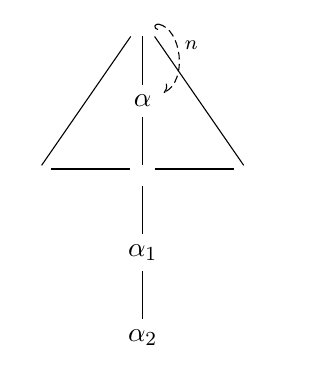
\includegraphics[scale =0.55]{figures/alpha.png}
\end{center}

  
\item Fórmulas de tipo \(\beta\). En cada rama abierta $r$ que tenga
  a profundidad menor o igual que \(n\) una fórmula de tipo \(\beta\)
  no desplegada, aplicamos a esa fórmula la regla \(\beta\):
 % https://tikzcd.yichuanshen.de/#N4Igdg9gJgpgziAXAbVABwnAlgFyxMJZARgBoAGAXVJADcBDAGwFcYkQQBfU9TXfQijLFqdJq3YAdSQCMYOelx4gM2PASLlSAJlEMWbRB2681AomV019Eo0tP8NKbTr3jDx5aseDkWgMxuBlKy8vQA+sT2Knzqvi6B1u4hcgrh2lyiMFAA5vBEoABmAE4QALZIWiA4EEhkYsGIYMyMjDSM9HKMAAqx5kaMMIU4IDQAFjD0UOyQYGwmICXllTQ1SC4Nts2t7Z0wPX1OIIPDoyATUzME88pLFYhVa4gALEmN223HewdmRycj40m0yMsxuRVK93qT38by2LU+HS6vV+gmOQwB5yBVzmZzkYGB5AWd3Wq1qiBhm0MH12SMOqP+ZwuwPA12ixPJpKQr0pSGpX1pKPYDMBlxBrKJEKQFKeAFYRczQWzJQ9OYh6njgQB2eqMLA4oxQehwCbTeXsMb0YoYAhMDEKLCMc0QCAAa1tZxsHkIEuWHOqZIAbGaxTjOJROEA
  \begin{center}
   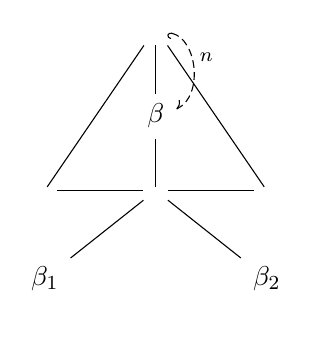
\includegraphics[scale =0.55]{figures/beta.png}
  \end{center}
  
\item Fórmulas de tipo \(\sigma\). En cada rama abierta $r$ que tenga
  a profundidad menor o igual que \(n\) una fórmula de tipo \(\sigma\)
  no desplegada, aplicamos a esa fórmula la regla \(\sigma\):
  
 % https://tikzcd.yichuanshen.de/#N4Igdg9gJgpgziAXAbVABwnAlgFyxMJZARgBoAGAXVJADcBDAGwFcYkQQBfU9TXfQijLFqdJq3YAdSdgDmAW3pceIDNjwEi5UgCZRDFm0QduvdQKJk9NAxOPKz-TSh2794oyZVqngkqQBmd0MpGSwFegB9Yi5RGChZeCJQADMAJwh5JG0QHAgkMjEQxDBmRkYaRnoAIxhGAAU+DUEQRhgUnBAaAAsYeih2SDA2UxB0zOyaPKRXIrtS8sqausbzZ1b2zp6+geMhkZVxrMQc6cQAFhsPJAWK1uWGpotjNo6ukF7+wYID1IzjwpnAJXYq3Ja1R5rFqvLYfHbfYbvWpgXbkUZHGZTfKIYFzIxg+4Q1a+dgw96fXbgH4OMb-JC4s6XPE3Mp3KpEp7rMnbL57anouknLEFGjI3YAdkKjCwiOMUHocF6Ax5lO69DSGAITFhOHoWEY7G6EAgAGtte9bJ5CAKJjjhYgAKwqhEjSicIA
  \begin{center}
    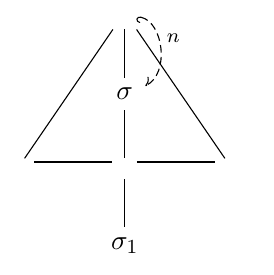
\includegraphics[scale =0.55]{figures/sigma.png}
  \end{center}
\item Fórmulas de tipo \(\delta\). En cada rama abierta $r$ que tenga
  a profundidad menor o igual que \(n\) una fórmula de tipo \(\delta\)
  no desplegada, aplicamos a esa fórmula la regla \(\delta\):
 % https://tikzcd.yichuanshen.de/#N4Igdg9gJgpgziAXAbVABwnAlgFyxMJZARgBoAGAXVJADcBDAGwFcYkQQBfU9TXfQijLFqdJq3YAdSbEY56XHiAzY8BIuVIAmUQxZtEHbr1UCiZHTT0TDik-3Uot23eINGlKh4JKkAzK76UjIwcvQAFADGAJRcojBQAObwRKAAZgBOEAC2SJogOBBIZGJBiGDMjIw0jPQARqEACnxqgiCMMGk4IDQAFjD0UOyQYGzGIJk5eTSFSM6lNhVVNfVNLWaGHV09IP2DwwRjSpO5iPmziAAsVm5IS9Xtq4zNpo7tnd19A0OGI0fpWVOJQufhuZXuKwaz3Wby2n123wOox2DTAP3I4xOcxmRUQoIWBghjyhL287DhOz2P3AhzsE0BSHxF2uBLulQetRJMLaFK++1+tMxDLOOOKNFRPwA7CVGFhkYYoPQ4P0hnzqb16BkMAQmPD5FhGOxehAIABrXU7azuQhCqZ40WIACsaqRY0onCAA
  \begin{center}
    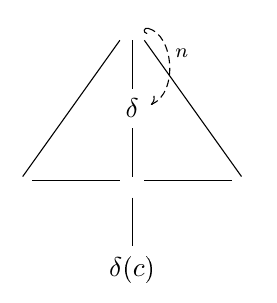
\includegraphics[scale =0.55]{figures/delta.png}
  \end{center}
\end{enumerate}

\subsubsection{EF-extensión}
Esta extensión la denominamos \(\mathbf{EF}(T,n)\). Consiste en añadir a cada
rama abierta $r$ de $T$ las fórmulas \(\varphi_{n}\in\Phi\) (según la numeración
del conjunto de fórmulas \(\Phi\)) y la fórmula \(\theta_{n}\in
EQ_{S}\) (según la numeración de las fórmulas de los axiomas de la
igualdad).
\begin{center}
  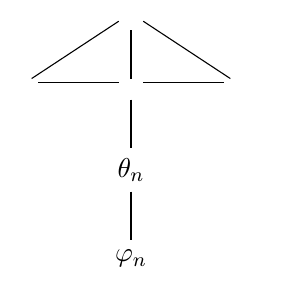
\includegraphics[scale = 0.55]{figures/ef.png}
\end{center}
\subsubsection{G-extensión}
Esta extensión se denota \(\mathbf{G}(T,n)\). Consiste en extender cada rama
abierta $r$ de $T$ con la fórmula \(\gamma_{i}(t_{j})\) donde el par \((i,j)\in \mathbb{N}\times\mathbb{N}\) es el menor par según el
  siguiente buen orden de \(\mathbb{N}\times\mathbb{N}\)
\[(i_{1},j_{1})< (i_{2},j_{2})\text{ sii }i_{1}+j_{1}<i_{2}+j_{2}\text{ o bien }i_{1}+j_{1}=i_{2}+j_{2}\text{ e }i_{1}<i_{2}\]
\begin{comment}
  \begin{displaymath}
    (i_{1},j_{1})< (i_{2},j_{2}) \quad\mbox{sii}\quad
    \left\{
      \begin{array}{ll}
        i_{1}+j_{1}<i_{2}+j_{2}\\
        i_{1}<i_{2} & \mbox{si}\ i_{1}+j_{1}=i_{2}+j_{2}
      \end{array}
    \right.
  \end{displaymath}
\end{comment}
 tal que $\gamma_{i}\in\Gamma_r$ está a altura $\leq n$,
  \(\gamma_{i}(t_{j})\not\in\Gamma_{r}\) y \(t_{j}\) es adecuado
  para \(\Gamma_{r}\). Si no hay ningún término adecuado para \(\Gamma_{r}\), aplicamos la regla considerando como término adecuado la primera constante auxiliar.
\end{itemize}
\begin{center}
  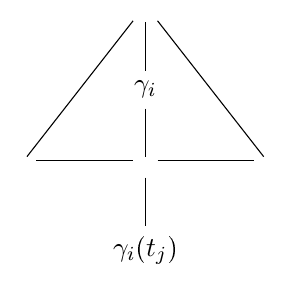
\includegraphics[scale = 0.55]{figures/gamma.png}
\end{center}

Por ejemplo,
supongamos \(\gamma_{0},\gamma_{2}\in\Gamma_{r}\) y
\(\gamma_{1}\not\in\Gamma_{r}\). Las fórmulas se van poniendo en el
siguiente orden en las ramas: \(\gamma_{0}(t_{0})\),
\(\gamma_{0}(t_{1})\), \(\gamma_{0}(t_{2})\) y \(\gamma_{2}(t_{0})\), donde hemos omitido las fórmulas con $\gamma_1$ ya que \(\gamma_{1}\not\in\Gamma_{r}\).


Veamos finalmente cómo se construye el \textit{tableau} canónico de una secuencia de fórmulas $\Phi=\{\varphi_1,\varphi_2,\dots\}$. Definimos la siguiente secuencia de árboles:
% https://tikzcd.yichuanshen.de/#N4Igdg9gJgpgziAXAbVABwnAlgFyxMJZABgBpiBdUkANwEMAbAVxiRAB136AnNACywB9YiAC+pdJlz5CKMgEYqtRizaccfGDjrCxSmFADm8IqABm3CAFskZEDghJ51TXShtIYVqIqigA
\begin{center}
$T_0 = $
\begin{tikzcd}
\varphi_0 \arrow[d, no head] \\
\theta_0                    
\end{tikzcd}
\end{center}
Luego definimos para $n\geq 1$:
\begin{displaymath}
  \begin{array}{l@{\ =\ }l}
    T_{n}^{1}& \mathbf{ABSD}(T_{n-1}, n)\\
    T_{n}^{2}& \mathbf{G}(T_{n}^{1}, n) \\
    T_{n} & \mathbf{EF}(T_{n}^{2}, n)\\
  \end{array}
\end{displaymath}

Tenemos así una secuencia de árboles
\begin{displaymath}
  T_{0}\subseteq T_{1}\subseteq\ldots T_{k}\subseteq T_{k+1}\subseteq\ldots
\end{displaymath}
El \textit{tableau} canónico de un conjunto de fórmulas \(\Phi\), que denotaremos
por \(T_{\Phi}\), se construye como se indica a continuación.
En la secuencia anterior se cumple una de las siguientes condiciones:
\begin{itemize}

\item Existe $n$ tal que \(T_{n}=T_{n+1}\) y $T_n$ no tiene fórmulas a altura $>n$. Eso significa, por como están definidas las reglas, que \(T_{k}=T_{k+1}\) para todo $k\geq n$. El \textit{tableau} canónico es
  $T_{\Phi}=T_{n}$
\item No se da el caso anterior. Entonces tenemos una secuencia infinita y el \textit{tableau} canónico es el límite de
todos los árboles
\begin{displaymath}
  T_{\Phi} = \bigcup_{i\in\mathbb{N}}T_{i}
\end{displaymath}
\end{itemize}

 \begin{comment}
\begin{prop}
 Sea $S$ una signatura y \(\Phi\subseteq FORM_S\). Consideremos la
  secuencia de árboles \(T_{i},\ i\in\mathbb{N}\) que da lugar al \textit{tableau}
  canónico.
  Sea \(n\in\mathbb{N}\) y $r$ una rama abierta de \(T_{n}\).Entonces la longitud de $r$ es mayor que $n$.

  \begin{center}
    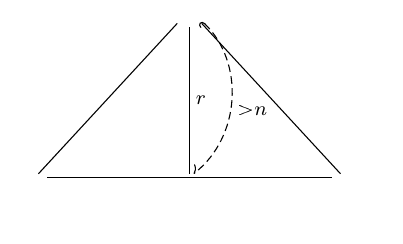
\includegraphics[scale= 0.6]{figures/prof.png}
  \end{center}
    \begin{proof}

  \end{proof}
  \end{comment}


\end{prop}


\begin{prop}
  Sea $S$ una signaturas, \(\Phi\subseteq FORM_S\), \(r\) una rama del
  \textit{tableau} canónico \(T_{\Phi}\) y \(\varphi\in\Gamma_{r}\) está a
  profundidad $k$. Entonces ha sido introducida en un paso $l<k$.
\end{prop}
  \begin{proof}
Lo probamos por inducción. En el caso 0 está claro que se cumple. Supongamos que se cumple para $n-1$. Sea $\varphi$ fórmula en $r$ a profundidad $k$, y supongamos que la hemos introducido en el paso $l\geq k$. Pues bien, la fórmula $\psi$ que está encima de $\varphi$, que está a altura $k-1$, ha tenido que ser introducida en la rama en un paso $\leq k-2$ por hipótesis de inducción. Esto significa que desde el \textit{tableau} $T_{l-2}$ a $T_{l-1}$ (es decir, en el paso $l-1$) no se ha añadido ningún elemento a esa rama. El resto se reduce a comprobar regla a regla que si una rama tiene longitud $l-1$ y no hemos añadido ninguna fórmula al aplicar la regla a esa rama en el paso $l-1$, entonces tampoco se añade ninguna fórmula al aplicar esa regla a la rama en el paso $l$, lo cual es una contradicción.
  \end{proof}
\end{corollary}

\begin{theorem}
  Sea $S$ una signaturas y \(\Phi\subseteq FORM_S\). El \texit{tableau} canónico
  \(T_{\Phi}\) es completo.

  \begin{proof}
    Sea $r$ una rama abierta de \(T_{\Phi}\). Hemos de demostrar
    \(\Phi\subseteq\Gamma_{r}\) y \(\Gamma_{r}\) es de Hintikka.\\
    Lo primero es fácil, dada \(\varphi\in\Phi\), existe un $k\in\N$
    tal que \(\varphi=\varphi_{k}\). Esa fórmula ha sido introducida en $r$ en el
    árbol \(T_{k}\) al aplicar la regla \(\mathbf{EF}(T_k^2,n)\), de modo que ya tenemos que $\Phi\subseteq\Gamma_{r}$.\\
    Para ver que \(\Gamma_{r}\) es de Hintikka, comprobamos primero que no puede darse $\bot\in\Gamma_r$ o $\varphi,\neg\varphi\in\Gamma_r$ para ninguna $\varphi$, ya que en ese caso $r$ sería una rama cerrada.
    Veamos que se cumplen el resto condiciones de la definición de Hintikka.
    \begin{description}
    \item[\(\alpha\)-saturación.] Tomemos \(\alpha\in\Gamma_{r}\). Esa
      fórmula estará a una profundidad \(k\) del árbol. Esa fórmula ha
      sido expandida en el el arbol $T_{k}$. Por tanto
      \(\alpha_{1},\alpha_{2}\in\Gamma_{r}\).\\

    \item[\(\beta\)-saturación, \(\sigma\)-saturación,
      \(\delta\)-saturación.] Similar al anterior.\\
    \item[$\gamma$-saturación.]


    Sea \(\gamma\in\Gamma_{r}\) y $t\in TERM_{\overline{S}}$ un
      término adecuado para \(\Gamma_{r}\). Existe
      $n\in\N$ de forma que $\gamma$ está en la rama $r$ en todos
      los \textit{tableaux} $T_{k}$ con $k\geq n$. \\[5pt]
      Además existen $i\in\N$ tal que $\gamma=\gamma_{i}$ (en la numeración de las
      \(\gamma\)-fórmulas) y $j\in\N$ tal que $t=t_{j}$ (en la
      numeración de los términos). Llamamos $l$ a la posición que ocupa el par $(i,j)$ en nuestro buen orden de \(\N\times\N\).\\[5pt]
      Por otro lado, como $t$ es adecuado para \(\Gamma_{r}\) y \(voc(t)\) y $var(t)$ son finitos, hay cierto $m$ tal que $voc(t)\subseteq voc(\Gamma_{r_m})$ y $var(t)\subseteq lib(\Gamma_{r_m})$, es decir, $t$ es adecuado para $\Gamma_{r_m}$, siendo $r_m$ la rama del \textit{tableau} $T_m$ que da lugar a $r$.\\[5pt]
      Tras haber definido $n,m$ y $l$, está claro que en el \textit{tableau} $T_{n+m}$ se cumple que $t$ es adecuado para $\Gamma_{r_{n+m}}$ y $\gamma\in\Gamma_{r_{n+m}}$. De modo que, tras aplicar $l$ veces más la regla \mathbf{G}, es decir, en el \textit{tableau} $T_{n+m+l}$, tenemos que haber añadido en cierto punto la fórmula $\gamma(t)$. Por tanto para todo término $t$ adecuado para $\Gamma_r$, $\gamma(t)$ estará incluida en la rama, como queríamos.
    \end{description}
  \end{proof}
\end{theorem}

\begin{cor} (Completitud)
  Sea $S$ signatura y \(\Phi\subseteq FORM_S\) tal que
  $\text{Insat}(\Phi)$. Entonces:
  \begin{enumerate}[label=\alph*)]
  \item $\Phi$ tiene un \textit{tableau} cerrado finito.
  \item Sea \(\varphi\in FORM_S\) tal que \(\Phi\models\varphi\). Entonces
    \(\Phi\vdash_{tb}\varphi\).
  \end{enumerate}
  \end{cor}

  \begin{proof}
    El segundo apartado es aplicación inmediata del primero al conjunto $\Psi=\Phi\cup\{\neg\varphi\}$. Así que
    demostraremos $b)$. Construimos el \textit{tableau} canónico
    \(T_{\Phi}\). Puesto que \(T_{\Phi}\) es completo para \(\Phi\),
    si \(T_{\Phi}\) tuviera una rama \(r\) abierta tendríamos
    \begin{itemize}
    \item \(\Phi\subseteq \Gamma_{r}\)
    \item \(\Gamma_{r}\) es de Hintikka y por tanto satisfactible.
    \end{itemize}
    Por tanto tendríamos que \(\Phi\) es satisfactible. Por tanto
    \(T_{\Phi}\) ha de ser cerrado. Por el lema \ref{cefi}, el tableau es finito.
  \end{proof}

\begin{theorem}(Teorema de compacidad)
  Sea $S$ una signatura, \(\Phi\subseteq FORM_S\).
  \begin{enumerate}[label=\alph*)]
  \item Si $\text{Insat}(\Phi)$, existe $\Phi_{\mathit{fin}}\subseteq\Phi$ finito tal
    que $\text{Insat}(\Phi_{\mathit{fin}})$.
  \item Si todo conjunto finito $\Phi_{\mathit{fin}}\subseteq\Phi$ verifica
    $Sat(\Phi_{\mathit{fin}})$, entonces $Sat(\Phi)$.
  \end{enumerate}
  \begin{proof}
    Puesto que \(\Phi\) es insatisfactible tiene un \textit{tableau} cerrado
    \(T\). Al ser cerrado, es finito. Consideramos entonces
    el conjunto
    \(\Phi_{\mathit{fin}}=\Phi\cap\Gamma_{T}\)\footnote{\(\Gamma_{T}\) es el
      conjunto de fórmulas que aparecen en el \textit{tableau} T.}.
    Veamos que verifica las propiedades buscadas:
    \begin{itemize}
    \item Es finito, al ser $T$ finito.
    \item \(\Phi_{\mathit{fin}}\subseteq\Phi\).
    \item $\text{Insat}(\Phi_{\mathit{fin}})$ puesto que \(T\) también es un \textit{tableau}
      para \(\Phi_{\mathit{fin}}\).
    \end{itemize}
    El segundo apartado es simplemente la afirmación contrarrecíproca del primero.
  \end{proof}
\end{theorem}



\begin{example}
Veamos un ejemplo de \textit{Tableau} canónico abierto. Este ejemplo no tiene funciones, ya que cuando hay funciones el \textit{Tableau} resultante es infinito, al haber infinitos términos que sustituir en las reglas \mathbf{G}. El tableaux siguiente corresponde al conjunto de fórmulas \[\Phi=\{\forall x\;P(x)\lor Q(x),\neg(\forall x\; P(x)\lor \forall x\; Q(x))\}=\{\varphi_0,\varphi_1\}\]
Veremos que este tableau es satisfactible, de modo que al acabar de desarrollarlo tendremos ramas abiertas que nos permitirán encontrar modelos que satisfagan $\Phi$.\\

Para simplificar el \textit{tableau}, al desarrollarlo se van a ignorar los axiomas de igualdad. Veremos que en este caso esto no va a ser un problema ya que vamos a poder encontrar los modelos igualmente.\\

También para simplificar, vamos a enumerar las fórmulas según su altura. Esto dará lugar a que haya varias fórmulas numeradas igual, pero no causará ambiguedades ya que en cada rama solo habrá una fórmula con cada número.\\

Otra anotación importante es que en la versión teórica del algoritmo, tenemos una numeración predefinida de los términos y de las $\gamma$-fórmulas. Sin embargo, en la práctica obviamente solo haremos \textit{tableaux} finitos. Como da igual cambiar el orden de finitos términos, podemos establecer el orden de los finitos términos o $\gamma$-fórmulas que usemos según nos convenga.\\

Se muestra primero el \textit{tableau} construido y a continuación explicamos su construcción paso a paso. 
\end{example}


\hspace{-2cm}
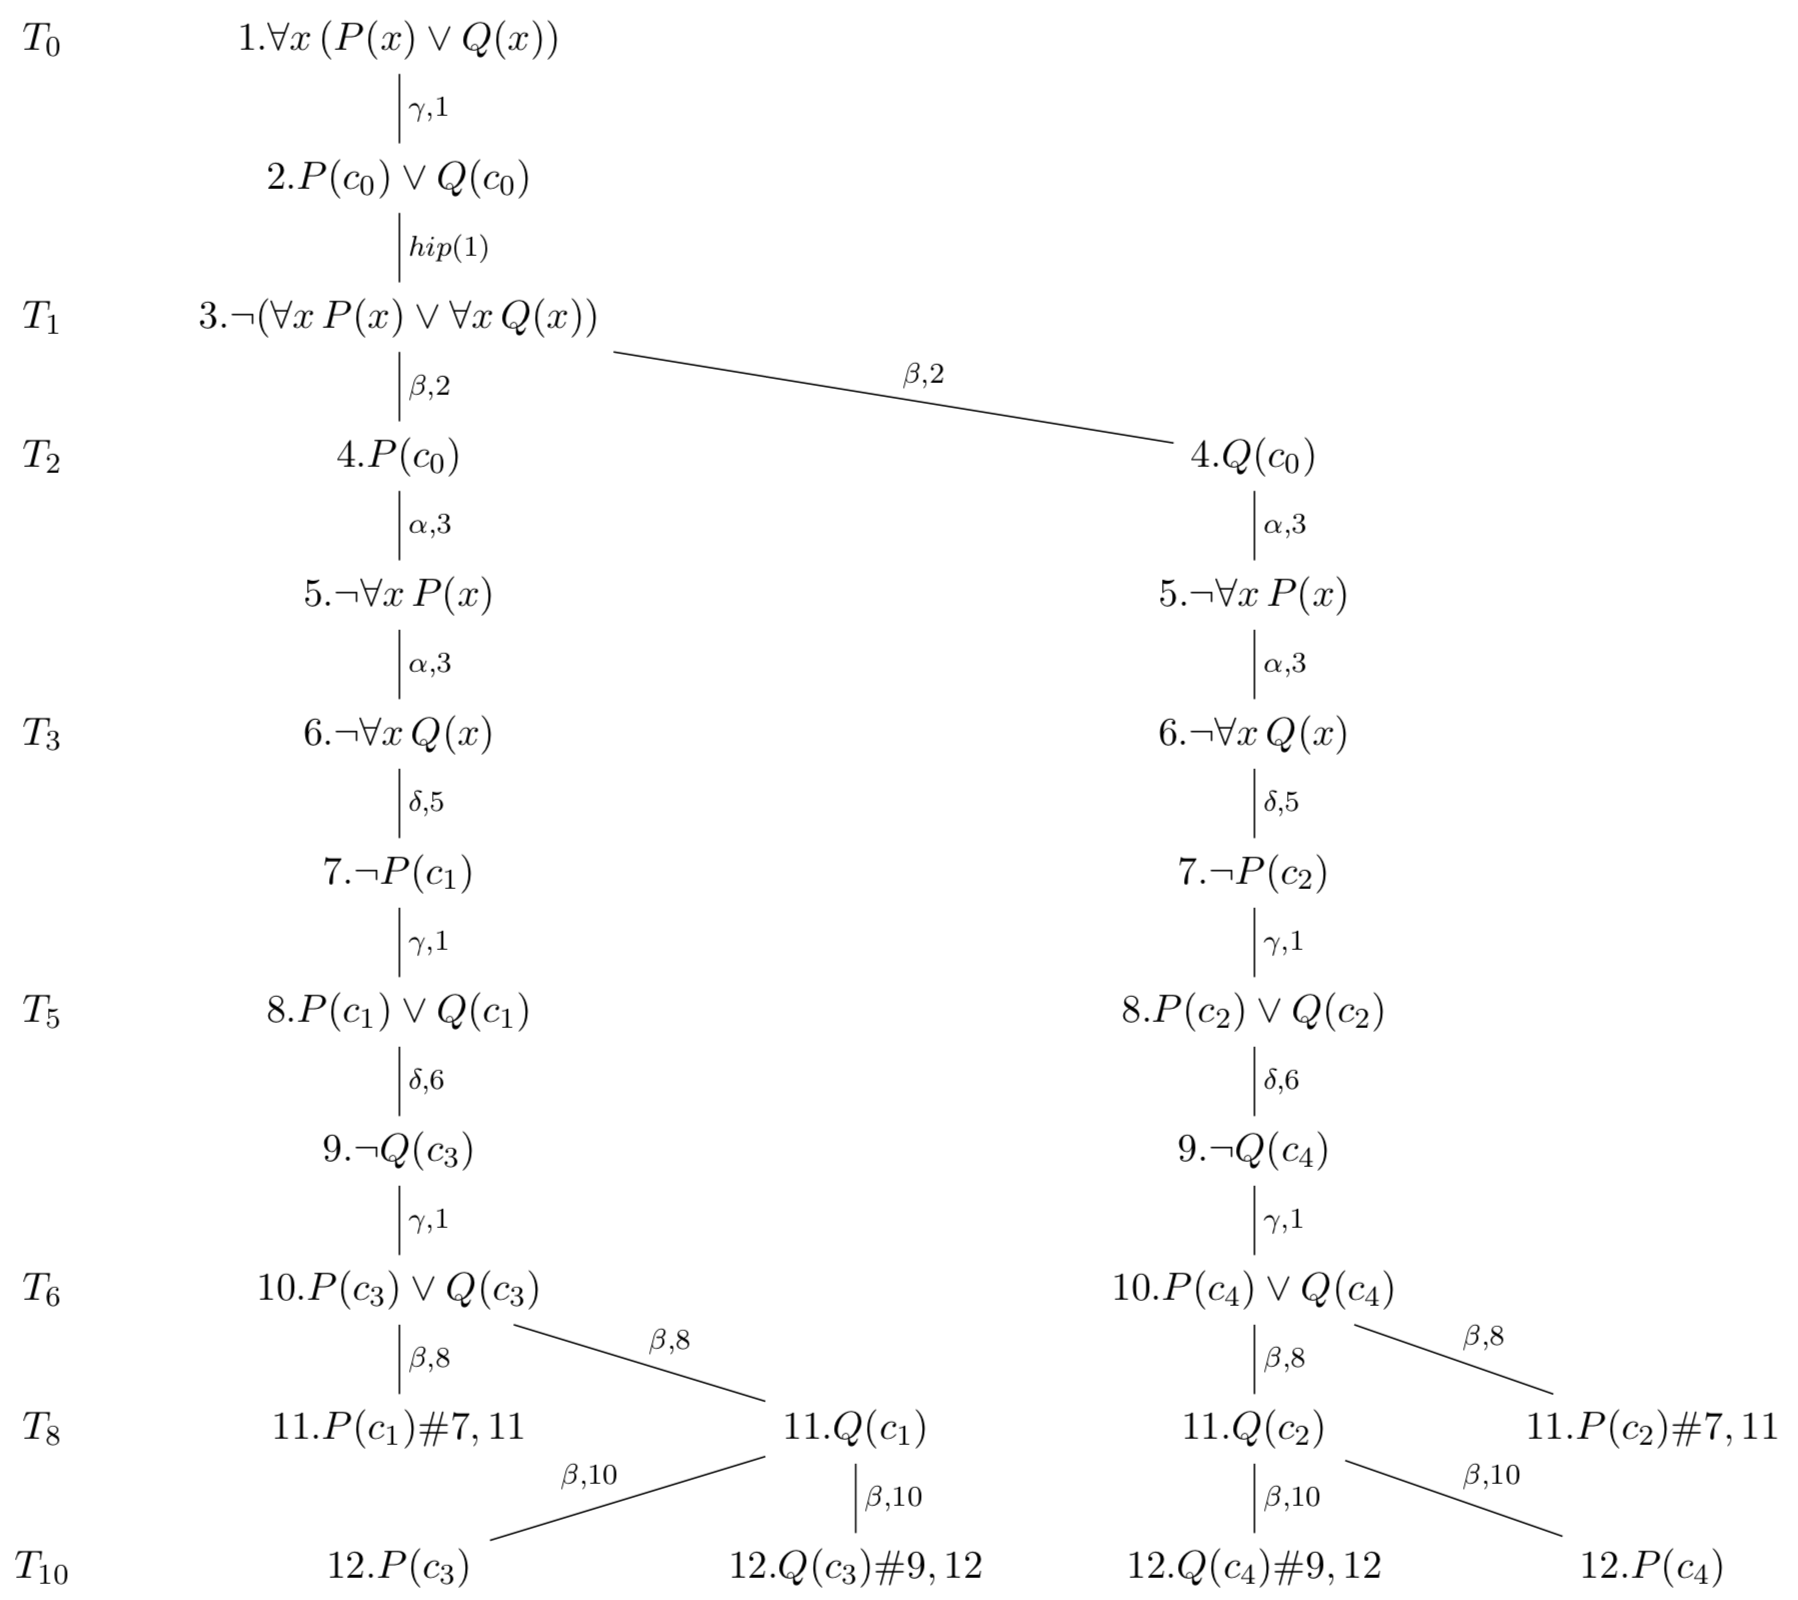
\includegraphics[scale = 0.5]{figures/tableau6.png}


\begin{comment}
% https://tikzcd.yichuanshen.de/#N4Igdg9gJgpgziAXAbVABwnAlgFyxMJZABgBpiBdUkANwEMAbAVxiRABUB9YkAX1PSZc+QigCM5KrUYs2AAjEA6OQB0VAMwgAnRgzkAPVStIAKAAon9ASiMNtcgIqWrVvgJAZseAkQlip9MysiCAATMoWAMbcNmp2Wo4m0cSu-IJeIkRkoQEywRycYm7pwj7ipDnUgbIhAMzKamAwAOYmapo6DHqGaqRyFta29u3augZGfU7Wqe6epaIkpLW5QWxcocUeQt4LEstVeWwALBFJMZtzO0S1Sys1ICeJyTMlV+VHd-kArA0qTc1GDpjHrGfrOC7bTIoG4fA6rEI-Iz-QGjLoGXpgwYQjJlRZfT5rTi1bHzXykfFw+4ANl+yJGnW6E0S1hJb2QNwp0nhIBpSJaKIZ4wxUxeWxxu1IVIJIQA7LT+VFCqLLlD2ZLpSA5XyAYrQsrIbiyDKNVwvqzVRJjZT8gAOU7RMSxFTxJ5K824m5Wrn3O1g6J6oYJJz+-Xisk2jUATnlAODRNDpOhpAj1rY0e1rqOCbZZEjJs4VPdErzqZCYmI9vjgddtWzqpuJe9+XLlaz1bjWaLWVI5fzNq75V7pZACiUfqVRgAxDK+mIimkxYnkKEe5Rh3PFHHHQO1UOm2wN669TujquNYfdVY1NPZ-PZgaFmQ5-ngOXeDu-P51+Fx7Wdyvn2-ZQ41ra9I1nDYFxVD0ey-fcyx-DsrxUSdwIUSD7zDFBT0A+CQDEH9FU7XgpBgKBmngIhQHULQIAAWyQCQQBwCAkBXPC1GaOg6LouhZxAagGDoAAjGAGDMB82AYGB1BwASQAACxgOgoDYSAmk2Gj6LY6gWKQU88IUrA0BMbdBJEsSJKwkBpNk+SlJUtSCFYBctIYxADL0xAqWHNRRJwPiNnM0TxMkkJbLk6gHNUkJ1Jc9w3P03TWMQGcOJUfy+LkIKbIs0LrIi+zlJi8BnM02j3J85iUptXyVEYNAFKy4lgsssKbJkyLFOKpyNNciqkDSrzwPShqmr6FrcpCqzEw6uyop62Kyv67TEFq6rGKY6p8jUMbmvkoTpvawqFscpa+oSgbEBGryCLqvaJoOvKZreOauui3r4uoq652SxibnS2AGACvozVa-LZpO7qztKi7vtWu6NsQMQDO2tg1CBkG5DBqa2oKzqiphuLyoRgHbqqtGQk47jeP48GXqhN7CZK4mVvclG-uRtLKZAameKyop6eOgnTpZ5bLoRqrbvWnmMbErHCyF-H5uhsW4ZARKuc5sQRtllRMayxXcYh16oY+86vo1n71q80ItsOKmVC4-m6eNhmyiZ0XPpJ9mbpS0J2L153aYUJ6juV97Fthy3NbtznQlRh3eYymAsf7JXIZF1XvbZtimNtr46syvp07d4WVfN6OfbY9jbYppO-NTrLS8OvHM4rqPWYl9yA-j7mG5TtOw7b02s8rrv4Z7wukdCXWB+LhQeAz16tCwZoFMjonxcntjp682oyHShfy2Hk3GbNzvt6t1bQillLant7lG6xk-l-PsfL-V2O76QWpA-npus4l5lwjszHOFBeBAA
\begin{tikzcd}
T_0    & { 1. \forall x \,(P(x) \lor Q(x))} \arrow[d, "{\gamma, 1}", no head]                                                   &                                                                                 &                                                                                           &                     \\
       & 2. P(c_0) \lor Q(c_0) \arrow[d, "hip(1)", no head]                                                                     &                                                                                 &                                                                                           &                     \\
T_1    & {3. \neg(\forall x \, P(x) \lor \forall x \, Q(x))} \arrow[d, "{\beta,2}", no head] \arrow[rrd, "{\beta, 2}", no head] &                                                                                 &                                                                                           &                     \\
T_2    & 4. P(c_0) \arrow[d, "{\alpha, 3}", no head]                                                                            &                                                                                 & 4. Q(c_0) \arrow[d, "{\alpha, 3}", no head]                                               &                     \\
       & {5. \neg \forall x \, P(x)} \arrow[d, "{\alpha, 3}", no head]                                                          &                                                                                 & {5. \neg \forall x\, P(x) } \arrow[d, "{\alpha, 3}", no head]                             &                     \\
T_3    & {6. \neg \forall x \, Q(x)} \arrow[d, "{\delta, 5}", no head]                                                          &                                                                                 & {6. \neg \forall x \, Q(x)} \arrow[d, "{\delta, 5}", no head]                             &                     \\
       & 7. \neg P(c_1) \arrow[d, "{\gamma, 1}", no head]                                                                       &                                                                                 & 7. \neg P(c_2) \arrow[d, "{\gamma, 1}", no head]                                          &                     \\
T_5    & 8. P(c_1) \lor Q(c_1) \arrow[d, "{\delta, 6}", no head]                                                                &                                                                                 & 8. P(c_2) \lor Q(c_2) \arrow[d, "{\delta, 6}", no head]                                   &                     \\
       & 9. \neg Q(c_3) \arrow[d, "{\gamma, 1}", no head]                                                                       &                                                                                 & 9. \neg Q(c_4) \arrow[d, "{\gamma, 1}", no head]                                          &                     \\
T_6    & 10. P(c_3) \lor Q(c_3) \arrow[d, "{\beta, 8}", no head] \arrow[rd, "{\beta, 8}", no head]                              &                                                                                 & 10. P(c_4) \lor Q(c_4) \arrow[d, "{\beta, 8}", no head] \arrow[rd, "{\beta, 8}", no head] &                     \\
T_8    & { 11. P(c_1) \#7, 11}                                                                                                  & 11.Q(c_1) \arrow[ld, "{\beta, 10}"', no head] \arrow[d, "{\beta, 10}", no head] & 11. Q(c_2) \arrow[d, "{\beta, 10}", no head] \arrow[rd, "{\beta, 10}", no head]           & {11. P(c_2)\#7, 11} \\
T_{10} & 12. P(c_3)                                                                                                             & {12. Q(c_3)\#9, 12}                                                             & {12. Q(c_4)\#9, 12}                                                                       & 12. P(c_4)         
\end{tikzcd}
\end{comment}

Comenzamos con la construcción:
\begin{itemize}
    \item $T_0$
    Inicializamos el \textit{tableau} con la primera fórmula de $\Phi$, $\varphi_0$. En el algoritmo completo tendríamos que tener el primer axioma de igualdad, pero como dijimos en la introducción vamos a omitirlos para simplificar.
    \item $T_1$
    \begin{itemize}
        \item \textbf{ABSD}$(T_0,1)$ No hay ninguna fórmula $\alpha,\beta,\sigma$ o $\delta$ que desarrollar a altura 1, de modo que seguimos.
        \item \textbf{G}($T_1^1$) Tenemos una fórmula $\gamma$ a altura $\leq 1$: $\varphi_0$. Como vamos a ir numerando las $\gamma$-fórmulas sobre la marcha, esta será la fórmula $\gamma_0$. Ahora buscamos términos adecuados para $\Gamma_r$. Sin embargo, vemos que no hay variables libres ni símbolos de constante en $\Gamma_r$, por tanto no se puede construir ningún término adecuado para $\Gamma_r$. Como no hay términos adecuados, usaremos la primera constante auxiliar, $c_0$. De modo que añadimos la fórmula $\gamma_0(c_0)$, que es $P(c_0)\lor Q(c_0)$.
        \item \textbf{EF}($T_1^2,1$) Añadimos la segunda fórmula de $\Phi$, $\varphi_1$. Como ya no quedan más fórmulas en $\Phi$ y no estamos usando axiomas de igualdad, no nos hará falta volver a usar la regla \textbf{EF} a partir de ahora.
    \end{itemize}
    Habiendo aplicado todas las reglas, ya tenemos el \textit{tableau} $T_1$. Comenzamos la siguiente fase para extender el \textit{tableau} a $T_2$.
    \item $T_2$
    \begin{itemize}
        \item \textbf{ABSD}$(T_1,2)$ Tenemos una $\beta$-fórmula en altura 2, $P(c_0)\lor Q(c_0)$. Por tanto, le aplicamos la regla $\beta$, dividiendo así el \textit{tableau} en dos ramas, $r_1$, con la fórmula $P(c_0)$, y $r_2$, con la fórmula $Q(c_0)$.
        \item \textbf{G}($T_2^1$) Como ya tenemos una constante, ya tenemos algún término adecuado: $c_0$. Ahora, la única $\gamma$-fórmula a altura $\leq2$ es $\varphi_0=\gamma_0$, pero ya hemos aplicado la regla a esa fórmula con el único término adecuado, $c_0$. Por tanto no añadimos nada en la regla \textbf{G}. Queda completado el \textit{tableau} $T_2$.
    \end{itemize}
    \item $T_3$
    \begin{itemize}
        \item \textbf{ABSD}$(T_2,1)$ En las ramas $r_1$ y $r_2$ tenemos en altura 3 la $\alpha$-fórmula, $\neg(\forall x \, P(x) \lor \forall x \, Q(x))$. Por tanto aplicamos la $\alpha$-fórmula en ambas ramas, añadiendo las fórmulas $\neg\forall x\, P(x)$ y $\neg\forall x\, Q(x)$.
        \item \textbf{G}($T_3^1$) Se da la misma situación que al construir $T_2$, no añadimos fórmulas en la regla \textbf{G}.
    \end{itemize}
    \item $T_4$
    \begin{itemize}
        \item \textbf{ABSD}$(T_3,4)$ No hay fórmulas $\alpha,\beta,\gamma,\delta$ a altura $4$ no extendidas.
        \item \textbf{G}($T_4^1$) Igual que antes no añadimos fórmulas en la regla \textbf{G}.
    \end{itemize}
    Como podemos observar, en el \textit{tableau} $T_4$ no hemos añadido ninguna fórmula nueva. Eso no significa que hayamos acabado, ya que quedan fórmulas a profundidad $>4$. Como tenemos fórmulas de altura hasta 6, tendríamos que llegar a $T_6$ sin ningún cambio para concluir que ya tenemos el \textit{tableau} canónico. Pero veremos que ese no es el caso.
    \item $T_5$
    \begin{itemize}
        \item \textbf{ABSD}$(T_4,5)$ En $r_1$ y $r_2$ tenemos a altura 5 la $\delta$-fórmula $\neg\forall x \, P(x)$. Por tanto, en $r_1$ añadimos la fórmula sustituyendo la primera constante auxiliar que no hemos usado, $c_1$. Es decir, prolongamos $r_1$ con la fórmula $\neg P(c_1)$. Ahora, en $r_2$, usamos la primera constante auxiliar que no habíamos usado hasta ahora, $c_2$, por tanto añadimos a la rama la fórmula $\neg P(c_2)$.\\
        \item \textbf{G}($T_5^1$) Seguimos teniendo una sola fórmula $\gamma$ a altura $\leq5$, que es $\gamma_0=\varphi_0$.\\[5pt]
        Al extender la rama $r_1$, hemos aumentado su vocabulario con un símbolo de constante nuevo: $c_1$. Por tanto tenemos un nuevo término, $c_1$. Como $\gamma_0(c_1)$ no está en $r_1$, añadimos $\gamma_0(c_1)=P(c_1)\lor Q(c_1)$ a $r_1$.\\[5pt]
        En $r_2$, análogamente a $r_1$, tenemos el nuevo término $c_2$, por tanto añadimos $\gamma_0(c_2)=P(c_2)\lor Q(c_2)$.
    \end{itemize}
    \item $T_6$
    \begin{itemize}
        \item \textbf{ABSD}$(T_5,6)$ Hay una $\delta$-fórmula a altura 6 que extender en cada rama, $\neg\forall x\,Q(x)$. Razonando como en $T_5$, a la rama $r_1$ le añadimos la fórmula $\neg Q(c_3)$ y a $r_2$ le añadimos la fórmula $\neg Q(c_4)$.
        \item \textbf{G}($T_6^1$) Igual que hicimos en $T_5$, $\gamma_0$ sigue siendo nuestra única $\gamma$-fórmula, y tenemos los nuevos términos $c_3$ y $c_4$ en $r_1$ y $r_2$ respectivamente, por tanto añadimos a $r_1$ la fórmula $\gamma_0(c_3)$ y añadimos a $r_2$ $\gamma_0(c_4)$.
    \end{itemize}
    \item $T_7$
    \begin{itemize}
        \item \textbf{ABSD}$(T_7,8)$ Ninguna fórmula que extender a altura 7.
        \item \textbf{G}($T_8^1$) De nuevo, en ambas ramas hemos agotado el vocabulario y ya no nos quedan términos adecuados que aplicar a $\gamma_0$, por tanto no añadimos ninguna fórmula.
    \end{itemize}
    \item $T_8$
    \begin{itemize}
        \item \textbf{ABSD}$(T_7,8)$ En $r_1$, tenemos una $\beta$-fórmula a altura 8, $P(c_1)\lor Q(c_1)$. De modo que obtenemos dos nuevas ramas. La de la izquierda, que se forma añadiendo $P(c_1)$, es una rama cerrada ya que contiene las fórmulas $P(c_1)$ y $\neg P(c_1)$. La de la derecha se forma añadiendo $Q(c_1)$.\\[5pt]
        En $r_2$, de igual forma, aplicamos la regla $\beta$ obteniendo dos ramas, una de las cuales se forma añadiendo $Q(c_2)$. La otra se forma añadiendo $P(c_2)$ y queda cerrada al contener a $P(c_2)$ y $\neg P(c_2)$.
        \item \textbf{G}($T_8^1$)Igual que en $T_7$, no añadimos nada.
    \end{itemize}
    \item $T_9$
    Al igual que en $T_4$ y $T_7$, ninguna de las reglas añade ninguna fórmula.
    \item $T_{10}$
    \begin{itemize}
        \item \textbf{ABSD}$(T_9,10)$ En la rama de la izquierda, aplicamos la regla $\beta$ a $P(c_3)\lor Q(c_3)$, obteniendo dos ramas. Una de ellas queda cerrada por contener a $Q(c_3)$ y a $\neg Q(c_3)$. En la rama de la derecha hay una situación similar.
        \item \textbf{G}($T_{10}^1$) Ninguna nueva $\gamma$-fórmula ni vocabulario nuevo en ninguna rama.
    \end{itemize}
    \item $T_{11}$ Ninguna regla añade nada nuevo.
    \item $T_{12}$ De nuevo, ninguna regla añade nada nuevo.\\[5pt]
    Sin embargo, nuestro \textit{tableaux} no tiene fórmulas a altura $>12$. Como además se cumple que $T_{11}=T_{12}$, hemos acabado y ya tenemos nuestro \textit{tableau} canónico.
\end{itemize}

Pues bien, ya tenemos el \textit{tableau} canónico asociado a $\Phi$. Nos quedan dos ramas abiertas. Llamamos al conjunto de fórmulas de la rama abierta de la izquierda $\Phi_1$ y al conjunto de fórmulas de la rama abierta de la derecha $\Phi_2$. Pues bien, como las ramas son abiertas en el \textit{tableau} canónico, $\Phi_1$ y $\Phi_2$ son de Hintikka. Por tanto, conforme a lo visto en la subsección \ref{Hinti33}, podemos crear modelos que satisfacen $\Phi_1$ y $\Phi_2$. Comenzamos con $\Phi_1$.\\[10pt]

En $\Phi_1$, los únicos símbolos de constante o variable que aparecen son $c_0,c_1$ y $c_3$. Como no hay símbolos de función, estos son nuestros únicos términos. Además, como no han aparecido igualdades en el \textit{tableau}, el conjunto soporte coincidirá con el conjunto de términos. Por tanto tenemos nuestro conjunto soporte:
\[T=\{c_0,c_1,c_3\}\]
Ahora, en esta rama solo tenemos dos predicados, $P$ y $Q$, ambos predicados $1$-arios. Para ver cuáles son sus interpretaciones, recordemos que dado un término $t$, definimos $P(t)=V$ si y solo si $P(t)$ aparece en la rama. Por tanto, $P$ será el conjunto de términos tales que $P(t)$ aparece en la rama. Las apariciones de $P$ en la rama son $P(c_0)$ en altura 4 y $P(c_3)$ en altura 12, por tanto:
\[P=\{c_0,c_3\}\]
De igual forma, la única aparición de $Q$ en la rama es $Q(c_1)$ en altura 11, por tanto:
\[Q=\{c_1\}\]\\[10pt]

El caso de $\Phi_2$ es similar al de $\Phi_1$. El conjunto soporte coincide con el conjunto de términos, en este caso como solo aparecen $c_0,c_2,c_4$:
\[T=\{c_0,c_2,c_4\}\]
Y $P$ solo aparece como $P(c_4)$, por tanto $P=\{c_4\}$.
$Q$ aparece como $Q(c_0)$ y $Q(c_2)$, por tanto $Q=\{c_0,c_2\}$.
\chapter{Deducción natural}

\section{Introducción}

En los anteriores capítulos hemos desarrollado unos sistemas formales fundamentados en semántica y valores de verdad, es decir, a cada fórmula le asociamos un valor de verdad, $V$ o $F$, que se puede obtener mediante interpretaciones. Sin embargo, si un objetivo de la lógica es formalizar razonamientos, nos interesa estudiar también un sistema formal centrado en cómo deducir unas proposiciones de otras, sin hacer falta la noción de verdad.\\

Por ejemplo, supongamos que queremos demostrar un teorema, que vendrá expresado por una fórmula $\psi$, y para deducirlo necesitamos unas fórmulas $\varphi_1,\varphi_2,\dots,\varphi_n$. Lo que queremos es una serie de reglas que nos digan cuándo una fórmula se deduce de otras, de modo que partiendo de unos axiomas y aplicando repetidamente estas reglas, podamos llegar en finitos pasos a que $\psi$ se deduce de $\varphi_1,\varphi_2,\dots,\varphi_n$.\\

De modo que nuestra intención ahora consiste en prestar atención a las \textit{reglas de inferencia}. Veremos a lo largo de este capítulo un sistema que solo conste de reglas de inferencia, así que comencemos por la siguiente


\begin{definition}
Una \textit{secuencia} es un par $\Gamma \idash \psi$ donde $\Gamma$ es un conjunto finito de fórmulas y $\psi$ es una fórmula que se denominan, respectivamente, \textit{conjunto de premisas} y \textit{conclusión}.
Normalmente, cuando $\Gamma$ es finito, denotamos la secuencia $\{\varphi_1, \dots, \varphi_n\} \idash \psi$ como $\varphi_1, \dots, \varphi_n \idash \psi$ y escribiremos $\Gamma, \varphi \idash \psi$ en vez de $\Gamma \cup \{\varphi\} \idash \psi$.
\end{definition}

Todas las reglas de nuestro sistema tendrán la forma:
\begin{prooftree}
\AxiomC{$\Gamma_1 \idash \varphi_1, \dots, \Gamma_n \idash \varphi_n$}
\UnaryInfC{$\Gamma \idash \varphi$}
\end{prooftree}
que intuitivamente significa: `se demuestra $\Gamma \idash \varphi$ si se demuestra cada secuencia $\Gamma_1 \idash \varphi_1, \dots, \Gamma_n \idash \varphi_n$'. \\[-5pt]

A lo largo de la exposición, veremos que existen reglas que no necesitan de premisas, que llamaremos \textit{axiomas}. En la siguiente sección exponemos las reglas y axiomas \textit{básicos}, y de ellos deduciremos después las reglas \textit{derivadas}.

\section{Reglas básicas}

\begin{itemize}
    \item[(\textbf{SP})] Axioma del supuesto: 
    \emph{si $\varphi\in\Gamma$, entonces $\Gamma\idash\varphi$ es un axioma.}
    
    \begin{center}
      \centerAlignProof
        (\textbf{SP})
      \quad
      \centerAlignProof
        \AxiomC{}
        \UnaryInfC{$\Gamma \idash \varphi$}
      \DisplayProof
      \quad
      \centerAlignProof
        $\varphi \in \Gamma$
    \end{center}
    

    \item[ (\textbf{FS})] Fortalecimiento del supuesto: 
    \emph{si $\Delta \idash \varphi$ y $\Gamma$ contiene a $\Delta$, se deduce $\Gamma \idash \varphi$.}
    \begin{center}
      \centerAlignProof
        (\textbf{FS})
      \quad
      \centerAlignProof
        \AxiomC{$\Delta \idash \varphi$}
        \UnaryInfC{$\Gamma \idash \varphi$}
      \DisplayProof
      \quad
      \centerAlignProof
        $\Delta \subseteq \Gamma$
    \end{center}

    \item[(\textbf{RC})] Razonamiento en cadena: 
    \emph{podemos demostrar un resultado intermedio $\psi$ y luego usarlo.}
\begin{prooftree}
\AxiomC{$\Gamma \idash \psi$}
\AxiomC{$\Gamma, \psi \idash \varphi$}
\BinaryInfC{$\Gamma \idash \varphi$}(\textbf{RC})
\end{prooftree}


    \item[ ($\land$\textbf{A})] Conjunción en el antecedente: 
    \begin{center}
      \centerAlignProof
        ($\land$\textbf{A})
      \quad
      \centerAlignProof
        \AxiomC{$\Gamma,\varphi,\psi \idash \chi$}
        \UnaryInfC{$\Gamma,\varphi\land\psi \idash \chi$}
      \DisplayProof
      \quad
      \centerAlignProof
    \end{center}


    \item[($\land$\textbf{C})] Conjunción en el consecuente.
\begin{prooftree}
\AxiomC{$\Gamma \idash \psi$}
\AxiomC{$\Gamma \idash \varphi$}
\BinaryInfC{$\Gamma \idash \psi \land \varphi$}($\land$\textbf{C})
\end{prooftree}

   \item[($\rightarrow \textbf{A}$)] Implicación en el antecedente: \emph{si tenemos una implicación
    en el antecedente, podemos intentar demostrar la premisa
    y entonces suponer el consecuente}.
  
  \begin{prooftree}
    \AxiomC{$\Gamma, \varphi \rightarrow \psi \idash \varphi$}
    \AxiomC{$\Gamma, \psi  \idash \chi$}
    \BinaryInfC{$\Gamma , \varphi \rightarrow \psi \idash \chi$}($\rightarrow \textbf{A}$)
   \end{prooftree}
   
   \item[($\rightarrow \textbf{C}$)] Implicación en el consecuente: \emph{ponemos el antecedente de la implicación en las premisas}.
   
   \begin{prooftree}
    \AxiomC{$\Gamma, \varphi \idash \psi$}
    \UnaryInfC{$\Gamma \idash \varphi \rightarrow \psi$}($\rightarrow \textbf{C}$)
   \end{prooftree}
   
   \item[($\lor \textbf{A}$)] Disyunción en el antecedente: \emph{si tenemos una distinción de casos hay que demostrar cada uno de los casos}.
   
   \begin{prooftree}
    \AxiomC{$\Gamma, \varphi \idash \chi$}
    \AxiomC{$\Gamma, \psi \idash \chi$}
    \BinaryInfC{$\Gamma, \varphi \lor\psi \idash \chi$}($\lor \textbf{A}$)
   \end{prooftree}
   
   \item[($\lor \textbf{C}_{1, 2}$)] Disyunción en el consecuente: \emph{basta demostrar uno de los elementos de la disyunción.} En realidad son dos reglas:
 
    \begin{center}
      \centerAlignProof
       ($\lor \textbf{C}_1$)
      \quad
      \centerAlignProof
        \AxiomC{$\Gamma \idash \varphi$}
        \UnaryInfC{$\Gamma \idash \varphi \lor \psi$}
      \DisplayProof
      \qquad
      \centerAlignProof
        ($\lor \textbf{C}_2$)
      \quad
      \centerAlignProof
      \AxiomC{$\Gamma \idash \psi$}
      \UnaryInfC{$\Gamma \idash \varphi \lor \psi$}
      \DisplayProof
    \end{center}
    
    \item[($\neg \textbf{A}$)] Negación en el antecedente.
   
   \begin{prooftree}
    \AxiomC{$\Gamma, \neg \varphi \idash \varphi$}
    \UnaryInfC{$\Gamma, \neg\varphi \idash \bot $}($\neg \textbf{A}$)
   \end{prooftree}
   
   \item[($\neg \textbf{C}$)] Negación en el consecuente.
   
   \begin{prooftree}
    \AxiomC{$\Gamma, \varphi \idash \bot$}
    \UnaryInfC{$\Gamma \idash \neg\varphi $}($\neg \textbf{C}$)
   \end{prooftree}
   
   \item[($\bot \textbf{A}$)] Axioma de contradicción en el antecente: \emph{si en el antecedente tenemos una contradicción podemos deducir cualquier cosa}.
 
   
   \begin{prooftree}
    \AxiomC{}
    \UnaryInfC{$\Gamma, \bot \idash \varphi $}($\bot \textbf{A}$)
   \end{prooftree}
   
   \item[(\textbf{DN}!)] Doble negación. 
   \begin{prooftree}
    \AxiomC{$\Gamma \idash \neg\neg\psi$}
    \UnaryInfC{$\Gamma \idash \psi $}(\textbf{DN}!)
   \end{prooftree}
   
   Esta regla se dice \emph{no constructiva}. La lógica intuicionista, por ejemplo, no la acepta. Escribiremos signos `!' en toda regla derivada que use $(\textbf{DN}!)$ en su demostración.
   
   \item[($\forall \textbf{A}$)] Fórmula universal en el antecente: \emph{la fórmula universal se puede aplicar a cualquier término}.
   
   \begin{center}
      \centerAlignProof
        ($\forall \textbf{A}$)
      \quad
      \centerAlignProof
        \AxiomC{$\Gamma, \forall x \varphi, \varphi[t/x] \idash \psi$}
        \UnaryInfC{$\Gamma, \forall x \varphi \idash \psi $}
      \DisplayProof
      \quad
      \centerAlignProof
        $t\in TERM_{\overline{S}}$
    \end{center}
    
    \item[($\forall \textbf{C}*$)] Fórmula universal en el consecuente: \emph{demostramos la fórmula para un elemento genérico}.
   
   \begin{center}
      \centerAlignProof
        ($\forall \textbf{C}*$)
      \quad
      \centerAlignProof
        \AxiomC{$\Gamma \idash \varphi[c/x]$}
        \UnaryInfC{$\Gamma \idash \forall x \varphi $}
      \DisplayProof
      \quad
      \centerAlignProof
        $c\in C_A \text{  nueva}$
    \end{center}
    
    \item[($\exists \textbf{A}*$)] Fórmula existencial en el antecente: \emph{sabemos que existe un elemento que cumple la propiedad, lo nombramos}.
   
   \begin{center}
      \centerAlignProof
        ($\exists \textbf{A}*$)
      \quad
      \centerAlignProof
        \AxiomC{$\Gamma, \varphi[c/x] \idash \psi$}
        \UnaryInfC{$\Gamma, \exists x \varphi \idash \psi $}
      \DisplayProof
      \quad
      \centerAlignProof
        $c\in C_A \text{  nueva}$
    \end{center}
    
    \item[($\exists \textbf{C}$)] Fórmula existencial en el consecuente: \emph{basta encontrar un elemento que cumple la propiedad}.
    
    \begin{center}
      \centerAlignProof
        ($\exists \textbf{C}$)
      \quad
      \centerAlignProof
        \AxiomC{$\Gamma \idash \varphi[t/x]$}
        \UnaryInfC{$\Gamma \idash \exists x \varphi $}
      \DisplayProof
      \quad
      \centerAlignProof
        $t\in TERM_{\overline{S}}$
    \end{center}
    
    \item[ (\textbf{ID})] Axioma de identidad.
    
    \begin{center}
      \centerAlignProof
        (\textbf{ID})
      \quad
      \centerAlignProof
        \AxiomC{}
        \UnaryInfC{$\Gamma \idash t \doteq t $}
      \DisplayProof
      \quad
      \centerAlignProof
        $t\in TERM_{\overline{S}}$
    \end{center}
    
    \item[(\textbf{SUST})] Sustitución: \emph{si quiero demostrar la propiedad para un término t y sabemos que es igual a s, basta demostrar la propiedad para s}
    
    \begin{center}
      \centerAlignProof
        (\textbf{SUST})
      \quad
      \centerAlignProof
        \AxiomC{$\Gamma \idash \varphi[s/x]$}
        \UnaryInfC{$\Gamma, t\doteq s \idash \varphi[t/x] $}
      \DisplayProof
      \quad
      \centerAlignProof
        $t,s\in TERM_{\overline{S}}$
    \end{center}
\end{itemize}
    Las propiedades simétrica y transitiva pueden deducirse de esta regla.
    
\section{Árboles de deducción}

Una vez descritas las reglas básicas y dada una secuencia, para verificar si tal secuencia es o no correcta la descomponemos en las reglas básicas conocidas, es decir, revertimos la aplicación de las reglas básicas. La siguiente definición aclara estas nociones:
\begin{definition}
Un \textit{árbol de deducción} para una secuencia $\Gamma \idash \psi$ es un árbol de forma que nos nodos están etiquetados con secuencias, la raíz es $\Gamma \idash \psi$ y, dados un nodo $\Gamma_0 \idash \psi_0$ y sus hijos:
\begin{center}
\begin{tikzcd}
                                           & \Gamma_0 \idash \psi_0 \arrow[rd, no head] &                        \\
\Gamma_1 \idash \psi_1 \arrow[ru, no head] & \cdots                                 & \Gamma_n \idash \psi_n
\end{tikzcd}
\end{center}
se cumple que
\begin{prooftree}
\AxiomC{$\Gamma_0 \idash \psi_0 \quad \cdots \quad \Gamma_n \idash \psi_n$}
\UnaryInfC{$\Gamma \idash \psi$}
\end{prooftree}
es una regla.
\end{definition}

\begin{definition} \hspace{1} \\
\begin{enumerate}
    \item  Una secuencia $\Gamma \idash \psi$ se dice \textit{formalmente deducible}, $\vdash \Gamma \idash \psi$, si existe un árbol de deducción para $\Gamma \idash \psi$ con axiomas en las hojas. Si $\Gamma = \emptyset$, en vez de $\Gamma \idash \psi$ escribimos $\vdash \psi$.
    \begin{center}
    % https://tikzcd.yichuanshen.de/#N4Igdg9gJgpgziAXAbVABwnAlgFyxMJZARgBoAGAXVJADcBDAGwFcYkQAdDgcXoFs+9AARcsUenAAWIjmmwgAvqXSZc+QinKli1Ok1bsAggA98gxcpAZseAkTI6aDFm0QgAdJ4sqb6ogCZtXWcDNxMzekVdGCgAc3giUAAzACcIPiQtEBwIJDI9FyQwZkZGGkZ6ACMYRgAFVVsNEEYYJJwQGkkYeih2SDA2JWS0jMQsnKQAZid9V2LS8qqa+t87Nxa2jpAunr6CQctU9LyaCcRpkCksTcQAWkDt7t63fsHKBSA
    \begin{tikzcd}
                                             & \Gamma \idash \psi \arrow[ld, no head] \arrow[rd, no head] &        \\
    Axioma \arrow[rr, no head, shift left=2] & Axiomas                                                       & Axioma
    \end{tikzcd}
    \end{center}
    
    \item Si $\Phi$ es un conjunto de fórmulas (no necesariamente finito) diremos que una fórmula $\varphi$ es \emph{formalmente deducible a partir de $\Phi$}, y denotado por $\Phi \vdash \varphi$, si existe un subconjunto finito $\Gamma \subset \Phi$ tal que $\vdash \Gamma \idash \varphi$
\end{enumerate}
\end{definition}
$\Phi \vdash \varphi$ y $\vdash \Phi \idash \varphi$ son equivalentes si $\Phi$ es finito. $\Phi \vdash \varphi$ permite que $\Phi$ sea infinito y con $\vdash \Phi\idash \varphi$ se asume la finitud de $\Phi$. \\ \\
Veamos un primer ejemplo detallado de árbol de deducción:
\begin{example}\label{primerejemplo} \hspace{1} \\
\begin{center}
  \begin{tikzpicture}[sibling distance=5cm]
  \node (1) {\(\varphi\lor\psi,\neg\psi\idash\varphi\)}
  child{node (2) {\(\varphi,\neg\psi\idash \varphi\)}}
  child{
    node (3) {\(\psi,\neg\psi\idash \varphi\)}
    child{
      node{\(\psi,\neg\psi\idash \bot\)}
      child{
        node (5){\(\psi,\neg\psi\idash \psi\)}
        edge from parent node[right]{$\regla{\neg A}$}
      }
    }
    child{node (4){\(\psi,\neg\psi,\bot\idash \varphi\)}}
  };
  \node [below=1mm of 1] {\(\regla{\lor\mathbf{A}}\)};
  \node [below=1mm of 2] {\(\regla{SP}\)};
  \node [below=1mm of 3] {\(\regla{RC}\)};
  \node [below=1mm of 4] {\(\regla{\bot A}\)};
  \node [below=1mm of 5] {\(\regla{SP}\)};
\end{tikzpicture}
\end{center}
En este ejemplo, queremos llegar a que $\vdash \Gamma \idash \varphi$, siendo $\Gamma=\{\varphi\lor\psi,\neg\psi\}$. Como tenemos una disyunción en el antecedente, $\varphi\lor\psi$, podemos dividir por casos según la regla $\regla{\lor\mathbf{A}}$. \\
En una rama, tenemos $\varphi,\neg\psi\idash \varphi$. Como la conclusión es una premisa, esta secuencia es un axioma por ($\mathbf{SP}$).\\
En la otra rama, tenemos $\psi,\neg\psi\idash \varphi$. Está claro que $\psi,\neg\psi$ tiene que llevar a una contradicción, pero no hay ninguna regla que nos permita acabar directamente. En este caso podemos usar la regla ($\mathbf{RC}$), demostrando primero el resultado intermedio $\bot$ y luego demostrando $\varphi$ usando $\bot$. Esto lleva a una nueva división en ramas.\\
En la primera rama, tenemos $\psi,\neg\psi\idash\bot$. Como tenemos la fórmula $\neg\psi$ en el antecedente y $\bot$ en la conclusión, aplicamos la regla ($\neg\mathbf{A}$). Así, llegamos a la secuencia $\psi,\neg\psi\idash\psi$, que es un axioma ($\mathbf{SP}$).\\
En la segunda rama, tenemos $\psi,\neg\psi,\bot\idash\varphi$. Esta regla es un axioma ($\bot\mathbf{A}$), y hemos acabado.

\end{example}

\begin{example} \hspace{1} \\
    \begin{center}
  \begin{tikzpicture}
    \node{\(\forall x\, p(x)\rightarrow q(x)\quad \bigl(\forall x\,
      p(x)\bigr)\rightarrow\bigl(\forall x\,q(x)\bigr)\)}
    child{
      node{\(\forall x\, p(x)\rightarrow q(x),
        \forall x\,p(x)\quad \forall x\,q(x)\)}
      child {
        node{\(\forall x\, p(x)\rightarrow q(x),
          \forall x\,p(x)\quad q(c)\)}
        child {
          node{\(\forall x\, p(x)\rightarrow q(x),
            \forall x\,p(x),p(c)\rightarrow q(c)\quad q(c)\)}
          child {
            node{\(\forall x\, p(x)\rightarrow q(x),
              \forall x\,p(x),p(c)\rightarrow q(c), p(c)\quad q(c)\)}
            child [sibling distance=5cm]{
              node (1) {\(p(c)\rightarrow q(c), p(c)\quad q(c)\)}
              child{
                node(2){\(p(c)\rightarrow q(c), p(c)\quad p(c)\)}
              }
              child{
                node (3){\(p(c)\rightarrow q(c), q(c)\quad q(c)\)}
              }
              edge from parent node[right]{\(\regla{FS}\)}
            }
            edge from parent node[right]{\(\regla{\forall A}\)}
          }
          edge from parent node[right]{\(\regla{\forall A}\)}
        }
        edge from parent node[right]{\(\regla{\forall C*}\)}
      }
      edge from parent node[right]{\(\regla{\rightarrow C}\)}
    }
    ;
    \node[below=0mm of 1]{\(\regla{\rightarrow A}\)};
    \node[below=0mm of 2]{\(\regla{SP}\)};
    \node[below=0mm of 3]{\(\regla{SP}\)};
  \end{tikzpicture}
\end{center}

\end{example}

\section{Reglas derivadas}
Al crear árboles de deducción, hay una serie de razonamientos que se aplican muy frecuentemente pero que no vienen expresados por ninguna regla básica. Por ejemplo, en el ejemplo \ref{primerejemplo} para deducir la secuencia $\psi,\neg\psi\idash\varphi$, que parece tan obvia como un axioma, hemos necesitados tres nodos extra. Podemos resumir razonamientos frecuentes de este tipo en reglas que no son básicas pero se pueden deducir de ellas:

\begin{definition}
Una regla 
\begin{prooftree}
\AxiomC{$\Gamma_1 \idash \varphi_1 \quad \cdots \quad \Gamma_n \idash \varphi_n$}
\UnaryInfC{$\Gamma \idash \varphi$}
\end{prooftree}
con $n\geq0$ es derivable si existe un árbol de deducción para $\Gamma \idash \varphi$ cuyas hojas son axiomas o de la forma $\Gamma_i \idash \varphi_i,i=1,\dots,n$.
\end{definition}

Ahora, si tenemos un árbol de deducción $T$ para $\Gamma\idash\varphi$ que usa reglas básicas y derivadas, también existirá un árbol de deducción para $\Gamma\idash\varphi$ que solo usa reglas básicas. Informalmente, para obtener este nuevo árbol, basta con buscar en el árbol un nodo $\Gamma_0\idash\varphi_0$ que se ha obtenido de sus hijos mediante una regla derivada. De modo que fijándonos en ese nodo y sus hijos, el árbol será algo así:
\begin{center}
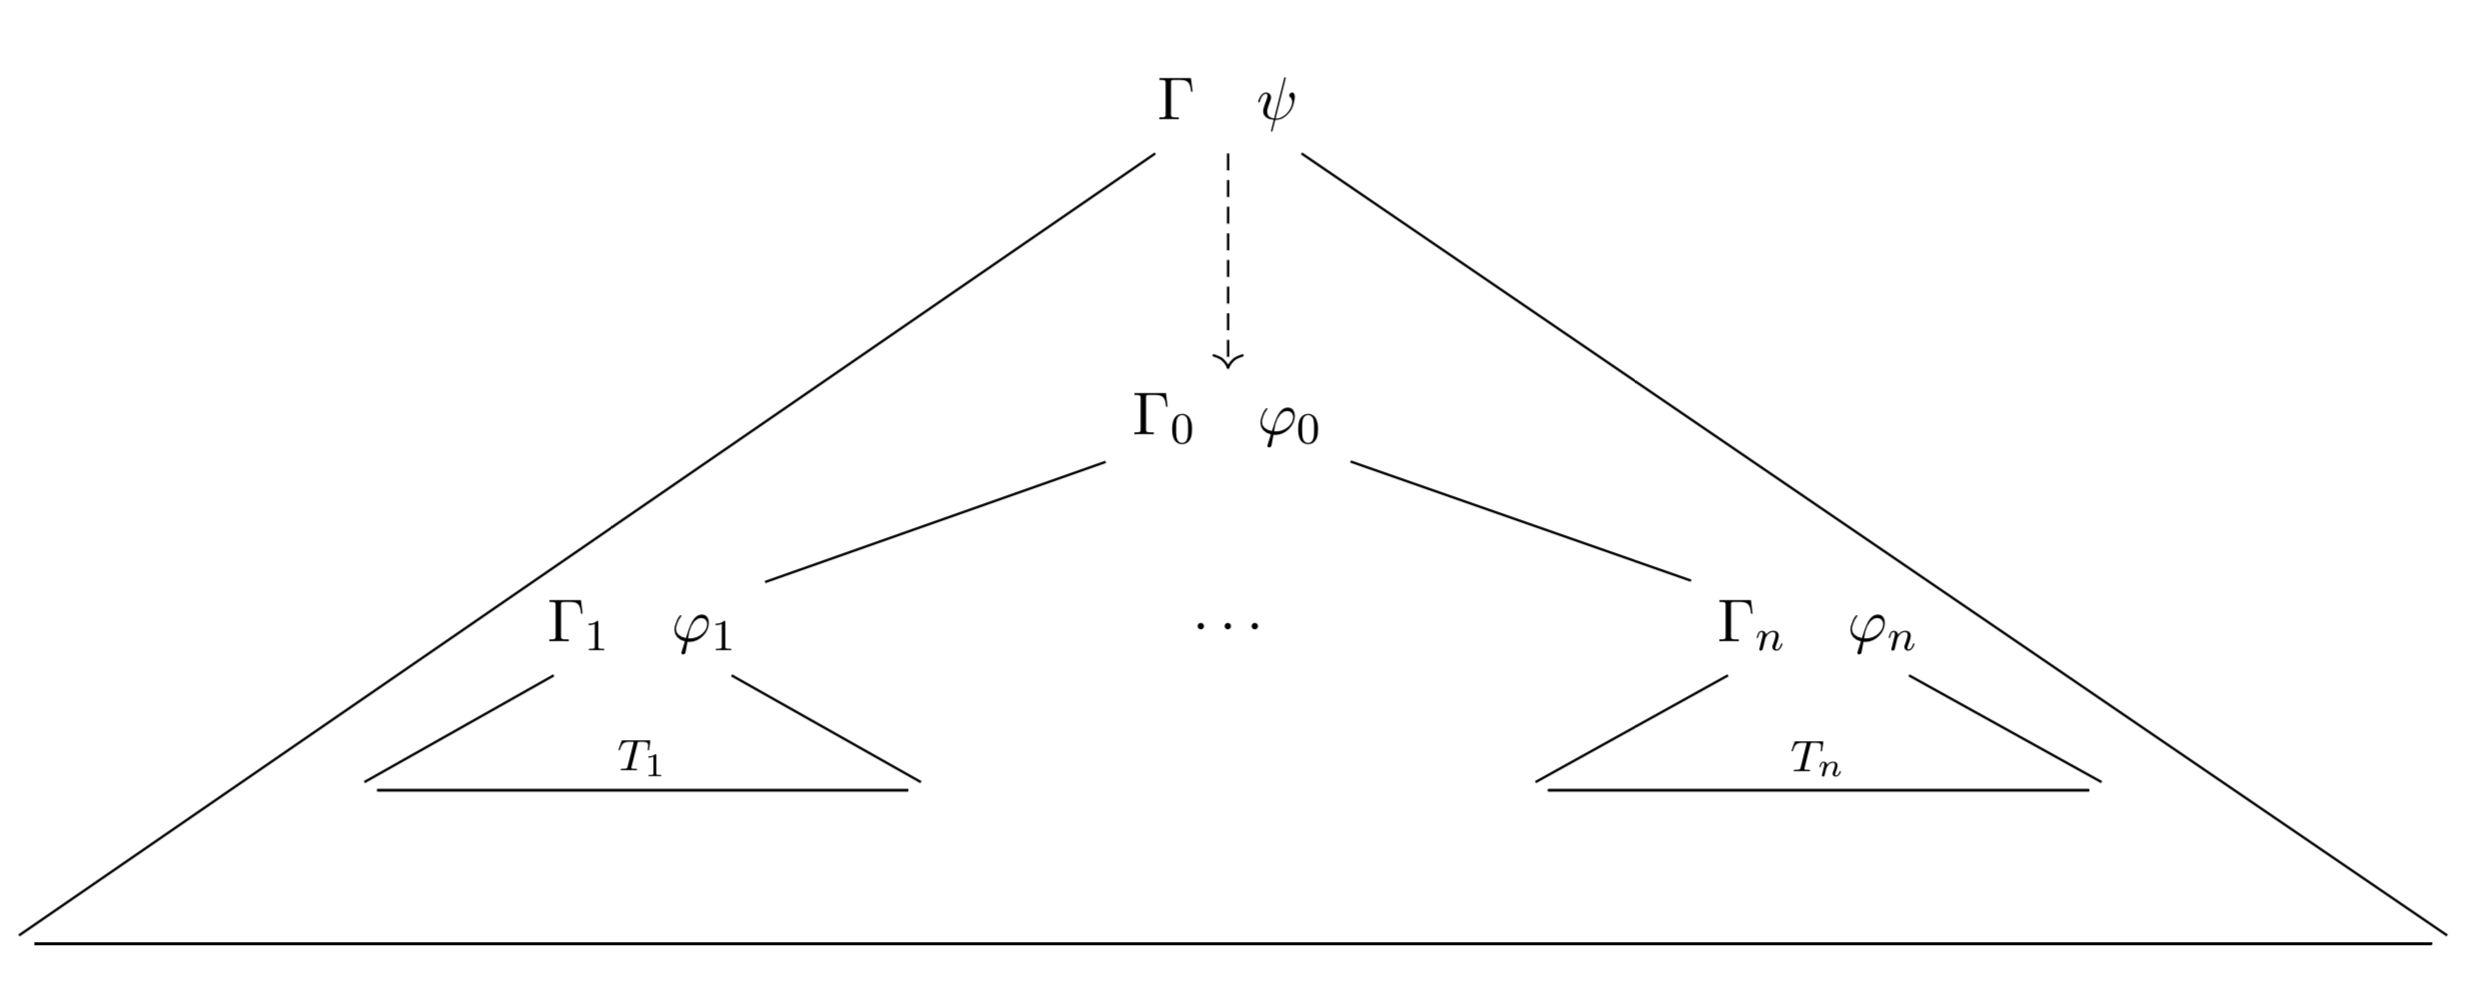
\includegraphics[scale = 0.3]{figures/arbol1.png}
% https://tikzcd.yichuanshen.de/#N4Igdg9gJgpgziAXAbVABwnAlgFyxMJZAVgBoAGAXVJADcBDAGwFcYkQAdDgcXoFs+9AARcsUenAAWIjmmwgAvqXSZc+QijIAmanSat2XXgPoB9cqPFSuDAE5pJWc4uUgM2PASIBmUt90MLGyInDz8gqYAjJYSkjb09o5RLioe6kQA7H4B+sGhxhFgMdYcdg5OhEqpal6a2TSBBiFcAMZQEDgIVW6qnhrIWqQALDlB7Ck9abXIQ8OjTSAT7jX9AGxzDbnj3ct9RAAcG3pjIUu96SjkpMTzeWdT-ZFXN5sniwq6MFAA5vBEoAAzWwQPhISI0HAQJBabpAkFgiFQxDeWHA0GIQYgSFIMggSQwehQdiQMBsVHwjGIpDrPEEokhElk1xw9G47GIGmMLCk9hwCBcok0fGE4kENgQ+hYRiink0Rj0ABGMEYAAVzrUQLYsN9JDgQDQpFgAXrEABaFHMtHUqmIXHC+ngMX6kCG41IXwgeVK1XqjSa7W652NPIAFWS5PRHvZWVpIoZToj7pth1jDsZExZSBj7JT9pl4pdjjdZotgKtiBT0aFdPzztdJo9XuVaoe7C1Or1rwWYcqlopVyxSPBICVYHpA65PJCVnxRMTiAH7IAnNW446efPF0OB3n4xu++iV4OwTua3uC-WkOb508bUfd+uL0WGx8FEA
\begin{comment}
\begin{tikzcd}
                               &  &                        &                                                                 &                                & \Gamma \quad \psi \arrow[dd, dashed] \arrow[lllllddddd, no head] \arrow[rrrrrddddd, no head] &                        &                                                                 &                                &  &                                \\
                               &  &                        &                                                                 &                                &                                                                                               &                        &                                                                 &                                &  &                                \\
                               &  &                        &                                                                 &                                & \Gamma_0\quad\varphi_0 \arrow[lld] \arrow[rrd]                                               &                        &                                                                 &                                &  &                                \\
                               &  &                        & \Gamma_1\quad\varphi_1 \arrow[ld, no head] \arrow[rd, no head] &                                & \cdots                                                                                        &                        & \Gamma_n\quad\varphi_n \arrow[ld, no head] \arrow[rd, no head] &                                &  &                                \\
                               &  & {} \arrow[rr, no head] &                                                                 & {} \arrow[ll, "A_1"', no head] &                                                                                               & {} \arrow[rr, no head] &                                                                 & {} \arrow[ll, "A_n"', no head] &  &                                \\
{} \arrow[rrrrrrrrrr, no head] &  &                        &                                                                 &                                &                                                                                               &                        &                                                                 &                                &  & {} \arrow[llllllllll, no head]
\end{tikzcd}
\end{comment}
\end{center}
donde $T_i$ es el árbol de deducción que se ha usado para llegar a $\Gamma_i\idash\varphi_i$. Ahora, simplemente, cambiamos el grafo formado por el nodo y sus $n$ hijos por el árbol de deducción de la regla derivada. Cuando en una hoja del árbol de la regla derivada aparece una secuencia $\Gamma_i\idash\varphi_i$, añadimos debajo de ella el árbol de deducción $T_i$. De modo que esquemáticamente obtenemos un árbol así:

\begin{center}
\begin{comment}
% https://tikzcd.yichuanshen.de/#N4Igdg9gJgpgziAXAbVABwnAlgFyxMJZAVgBoAGAXVJADcBDAGwFcYkQAdDgcXoFs+9AARcsUenAAWIjmmwgAvqXSZc+QijIAmanSat2XXgPoB9cqPFSuDAE5pJWc4uUgM2PASIBmUt90MLGyInDz8gqZYXACOzPRQNvT2jpEuKh7qRADsfgH6waHGEQBWMXEJHHYOTsVpbqqeGshapAAseUHsde5qXiitbR0GId0NmSgAbIM0gcMgoxl9yAAc03qdI0rpvU3kpMRDBQs7RACMewcz+V1b9YtNZP5XGyAAggAe+IIICrowUABzeBEUAAM1sED4SFONBwECQLRAkhg8XYkDAbBoUiwoJw0Nu4Mh0Nh8MQviRKKgaIImJA2NxSAAtKcCRCoYhEXCkAMKaiQui2KyiRySUgyLyqfyaXVCeyeVzEOLGFgMew4BBlVSaMi+eBpbD6FhGNTVTRGPQAEYwRgABTGfRAtiwAMkeKxjgZiHIQvZ4oVPJ1kr1prpHrxXrNlutdvu7CdLrd6zmABVUj6kOSFVMJSbacrVSF1ZqQAajbmSyBzVbbfaNI7na6ZWyM6LEDkc1LVenENmFe3A+X3Tjw97XLKkO2s9rKYPQ8OkHtK1Ga7GQvHG88U6Zat3FwqYSArWBJYv8wUrMiqbvW6sO8HBWPmxGQAqAJzT3UCpvC29vj9Br8h09UcwSfd8X1JW8B07Wl6RHbtOVJcloPvCs4KZbxu0zUlEXQsl-1nWYCmTCsq2jWs4wbPFfgUIA
\begin{tikzcd}
                               &  &                        &                                                                                                    &                                & \Gamma \idash \psi \arrow[dd, dashed] \arrow[lllllddddd, no head] \arrow[rrrrrddddd, no head] &                        &                                                                                                           &                                &  &                                \\
                               &  &                        &                                                                                                    &                                &                                                                                               &                        &                                                                                                           &                                &  &                                \\
                               &  &                        &                                                                                                    &                                & \Gamma_0\idash\varphi_0 \arrow[lld, no head, shift right] \arrow[rrd, no head, shift left]    &                        &                                                                                                           &                                &  &                                \\
                               &  &                        & \Gamma_i\quad\varphi_i \arrow[ld, no head] \arrow[rd, no head] \arrow[rrrr, no head, shift left=3] &                                & Axiomas                                                                                       &                       & \Gamma_j\quad\varphi_j \arrow[ld, no head] \arrow[rd, no head] \arrow[llll, "T"', no head, shift right=3] &                                &  &                                \\
                               &  & {} \arrow[rr, no head] &                                                                                                    & {} \arrow[ll, "T_i"', no head] &                                                                                               & {} \arrow[rr, no head] &                                                                                                           & {} \arrow[ll, "T_j"', no head] &  &                                \\
{} \arrow[rrrrrrrrrr, no head] &  &                        &                                                                                                    &                                &                                                                                               &                        &                                                                                                           &                                &  & {} \arrow[llllllllll, no head]
\end{tikzcd}
\end{comment}
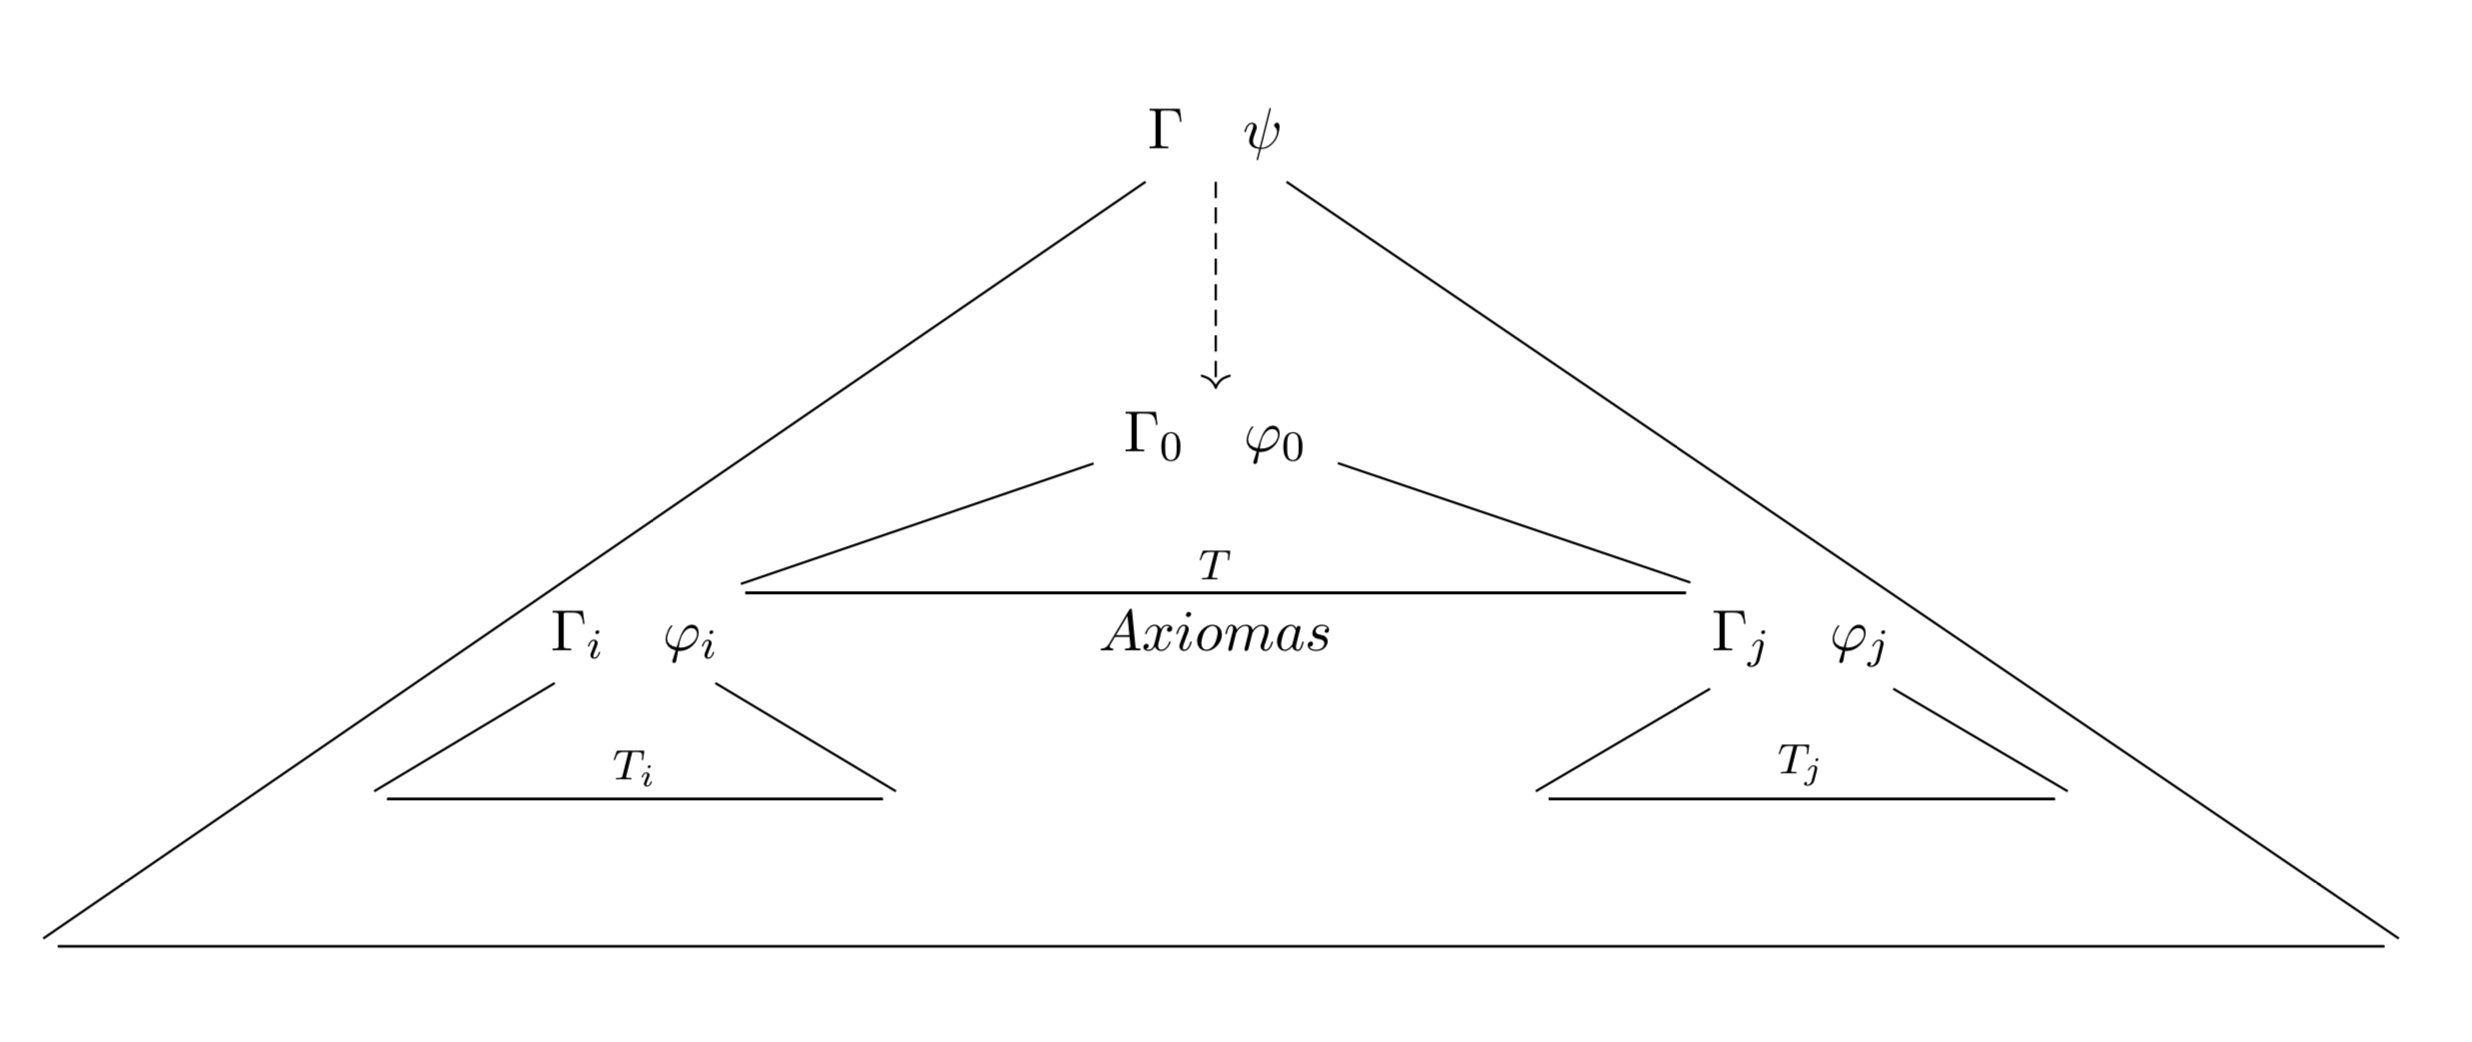
\includegraphics[scale = 0.3]{figures/arbol2.png}
\end{center}
donde en el árbol $T$ solo se usan reglas básicas y axiomas. Se puede demostrar que sustituyendo de este modo todas las reglas derivadas acabamos obteniendo un árbol en el que solo hay reglas básicas y axiomas.\\[10pt]
De modo que por lo que acabamos de ver, si tenemos un árbol para $\Gamma\idash\varphi$ que usa reglas básicas y derivadas, se cumple que $\Gamma\idash\varphi$ es formalmente deducible. Esto quiere decir que podemos usar sin problemas reglas derivadas que conocemos en los árboles de deducción.

\subsection{Repertorio de reglas derivadas}
En esta sección expondremos muchas reglas derivadas que permiten ver cómo razonamientos que hacemos habitualmente se expresan en el cálculo de secuencias. Para cada regla derivada incluímos su árbol de deducción.

\begin{itemize}
    \item Eliminación de una conjunción: \emph{siempre podemos demostrar un resultado más fuerte}. Son dos reglas simétricas.
    \begin{center}
      \centerAlignProof
       ($\textbf{E} \land$)
      \quad
      \centerAlignProof
        \AxiomC{$\Gamma \idash \psi\land\varphi$}
        \UnaryInfC{$\Gamma \idash \varphi $}
      \DisplayProof
      \qquad
      \centerAlignProof
        \AxiomC{$\Gamma \idash \varphi\land\psi$}
        \UnaryInfC{$\Gamma \idash \varphi $}
      \DisplayProof
    \end{center}
    \begin{proof} \hspace{1}
          \begin{center}
            \begin{tikzpicture}[sibling distance=5cm]
          \node (1) {\(\Gamma\idash \varphi\)}
              child{
                node (2){\(\Gamma\idash \psi\land\varphi\)}
              }
              child{
                node{\(\Gamma,\psi\land\varphi\idash \varphi\)}
                child{
                  node (3){\(\Gamma,\psi,\varphi\idash \varphi\)}
                  edge from parent node [right]{\(\regla{\land A}\)}
                }
              };
              \node[below=0mm of 1] {\(\regla{RC}\)};
              \node[below=0mm of 2] {Premisa};
              \node[below=0mm of 3] {\(\regla{SP}\)};
            \end{tikzpicture}
          \end{center}
    \end{proof}
    
    \item Modus Ponens
    \begin{center} 
      \centerAlignProof
       ($\textbf{MP}$)
      \quad
      \centerAlignProof
        \AxiomC{$\Gamma \idash \varphi \qquad \Gamma \idash \varphi \rightarrow \psi$}
        \UnaryInfC{$\Gamma \idash \psi $}
      \DisplayProof
    \end{center}
    \begin{proof} \hspace{1}
        \begin{center}
    \begin{tikzpicture}[sibling distance=5cm]
      \node (1){\(\Gamma\idash \psi\)}
      child{
        node (2){\(\Gamma\idash \varphi\)}
      }
      child{
        node (3){\(\Gamma,\varphi\idash \psi\)}
        child{
          node (4){\(\Gamma,\varphi,\varphi\rightarrow\psi\idash\psi\)}
          child{
            node
            (6){\(\Gamma,\varphi,\varphi\rightarrow\psi\idash\varphi\)}
          }
          child{node (7){\(\Gamma,\psi\idash\psi\)}}
        }
        child{
          node {\(\Gamma,\varphi\idash\varphi\rightarrow\psi\)}
          child{
            node(5){\(\Gamma\idash\varphi\rightarrow\psi\)}
            edge from parent node[right]{\(\regla{FS}\)}
          }
        }
      };
      \node[below=0mm of 1] {\(\regla{RC}\)};
      \node[below=0mm of 2] {Premisa};
      \node[below=0mm of 3] {\(\regla{RC}\)};
      \node[below=0mm of 4] {\(\regla{\rightarrow A}\)};
      \node[below=0mm of 5] {Premisa};
      \node[below=0mm of 6] {SP};
      \node[below=0mm of 7] {SP};

    \end{tikzpicture}
  \end{center}
    \end{proof}
    \item Variante de la conjunción en el consecuente.
    \begin{center} 
      \centerAlignProof
       ($\land \textbf{C}'$)
      \quad
      \centerAlignProof
        \AxiomC{}
        \UnaryInfC{$\Gamma, \varphi, \psi \idash \varphi\land\psi $}
      \DisplayProof
    \end{center}
    \begin{proof} \hspace{1}
         \begin{center}
            \begin{tikzpicture}[sibling distance=5cm]
              \node (1){\(\Gamma,\varphi,\psi\idash \varphi\land\psi\)}
              child{
                node (2) {\(\Gamma,\varphi,\psi\idash \varphi\)}
              }
              child{
                node (3) {\(\Gamma,\varphi,\psi\idash \psi\)}
              };
              \node[below=0mm of 1]{\(\regla{\land C}\)};
              \node[below=0mm of 2]{\(\regla{SP}\)};
              \node[below=0mm of 3]{\(\regla{SP}\)};
            \end{tikzpicture}
          \end{center}
    \end{proof}
    
    \item Variante de la disyunción en el consecuente.
    \begin{center} 
      \centerAlignProof
       ($\lor \textbf{C}'$)
      \quad
      \centerAlignProof
        \AxiomC{}
        \UnaryInfC{$\Gamma, \varphi \idash \varphi\lor\psi $}
      \DisplayProof
      \quad
      \centerAlignProof
        \AxiomC{}
        \UnaryInfC{$\Gamma, \psi \idash \varphi\lor\psi $}
      \DisplayProof
    \end{center}
    \begin{proof} \hspace{1}
         \begin{center}
            \begin{tikzpicture}
              \node{\(\Gamma,\varphi\idash \varphi\lor\psi\)}
              child{
                node(1){\(\Gamma,\varphi\idash \varphi\)}
                edge from parent node[right]{\(\regla{\lor C}\)}
              }
              ;
              \node[below=0mm of 1]{\(\regla{SP}\)};
            \end{tikzpicture}
          \end{center}
    \end{proof}
    
    \item Reducción al absurdo: \emph{suponer la negación de la conclusión y llegar a una contradicción}.
    \begin{center} 
      \centerAlignProof
       ($\textbf{RA}!$)
      \quad
      \centerAlignProof
        \AxiomC{$\Gamma,\neg \varphi \idash \bot$}
        \UnaryInfC{$\Gamma \idash \varphi $}
      \DisplayProof
    \end{center}
    \begin{proof} \hspace{1}
        \begin{center}
        \begin{tikzpicture}
          \node{\(\Gamma\idash \varphi\)}
            child{
              node{\(\Gamma\idash \neg\neg\varphi\)}
              child{
                node (1){\(\Gamma,\neg\varphi\idash\bot\)}
                edge from parent node[right]{\(\regla{\neg C}\)}
              }
              edge from parent node[right]{\(\regla{DN!}\)}
            }
            ;
            \node[below=0mm of 1]{Premisa};
        \end{tikzpicture}
      \end{center}
    \end{proof}
    
    \item Reglas de la contradicción.
    \begin{center} 
      \centerAlignProof
       ($\textbf{CT}_1$)
      \quad
      \centerAlignProof
        \AxiomC{$\Gamma \idash \psi \qquad \Gamma \idash \neg\psi$}
        \UnaryInfC{$\Gamma \idash \varphi $}
      \DisplayProof
    \end{center}
    
    \begin{proof} \hspace{1}
        \begin{center}
        \begin{tikzpicture}[sibling distance=5cm]
          \node(0){\(\Gamma\idash \varphi\)}
            child{
              node(1){$\Gamma, \bot \idash \varphi$}
            }
            child{
              node(2){$\Gamma \idash \bot$}
              child{
                  node(3){$\Gamma, \neg \psi \idash \bot$}
                  child {
                        node(5){$\Gamma, \neg \psi \idash \psi$}
                        child {
                            node(6){$\Gamma\idash \psi$}
                            edge from parent node[right]{\(\regla{FS}\)}
                        }
                        edge from parent node[right]{\(\regla{\neg A}\)}
                  }
              }
              child{
                  node(4){$\Gamma \idash \neg \psi$}
              }
            }
            ;
            \node[below=0mm of 0]{(\textbf{RC})};
            \node[below=0mm of 1]{($\bot$ \textbf{A})};
            \node[below=0mm of 2]{(\textbf{RC})};
            \node[below=0mm of 4]{Premisa};
            \node[below=0mm of 6]{Premisa};
        \end{tikzpicture}
      \end{center}
    \end{proof}
    
    \begin{center} 
      \centerAlignProof
       ($\textbf{CT}_2$)
      \quad
      \centerAlignProof
        \AxiomC{}
        \UnaryInfC{$\Gamma, \varphi, \neg\varphi \idash \psi $}
      \DisplayProof
    \end{center}
    
        \begin{proof} \hspace{1}
        \begin{center}
        \begin{tikzpicture}[sibling distance=4cm]
            \node(0){$\Gamma, \varphi, \neg\varphi \idash \psi$}
            child {
                node(1){$\Gamma, \varphi, \neg \varphi, \idash \neg \varphi$}
            }
            child {
                node(2){$\Gamma, \varphi, \neg \varphi, \idash \varphi$}
            }
            ;
            \node[below=0mm of 0]{($\textbf{CT}_1$)};
            \node[below=0mm of 1]{(\textbf{SP})};
            \node[below=0mm of 2]{(\textbf{SP})};
        \end{tikzpicture}
      \end{center}
      
      
    \end{proof}
    \item  Reglas de la doble negación.
    
    \begin{center} 
      \centerAlignProof
       ($\neg\neg\textbf{C}$)
      \quad
      \centerAlignProof
        \AxiomC{$\Gamma \idash \varphi$}
        \UnaryInfC{$\Gamma \idash \neg\neg\varphi $}
      \DisplayProof
      \qquad 
      \centerAlignProof
       ($\neg\neg\textbf{A}!$)
      \quad
      \centerAlignProof
        \AxiomC{$\Gamma,\varphi\idash \psi$}
        \UnaryInfC{$\Gamma,\neg\neg\varphi\idash \psi$}
      \DisplayProof
    \end{center}
    
    \begin{proof} \hspace{1}
        \begin{center}
        \begin{tikzpicture}[sibling distance=4cm]
            \node(0){$\Gamma \idash \neg\neg\varphi$}
            child{
                node(1){$\Gamma\idash \varphi$}
            }
            child {
                node(2){$\Gamma,\varphi \idash \neg\neg \varphi$}
                child {
                    node(3) {$\Gamma,\varphi,\neg\varphi \idash \bot$}
                    edge from parent node[right]{\(\regla{\neg C}\)}
                }
            }
            ;
            \node[below=0mm of 0]{($\textbf{RC}$)};
            \node[below=0mm of 1]{Premisa};
            \node[below=0mm of 3]{($\textbf{CT}_2$)};
        \end{tikzpicture}
        \end{center}
        \begin{center}
        \begin{tikzpicture}[sibling distance=4cm]
            \node(0){$\Gamma,\neg\neg\varphi\idash \psi$}
            child{
                node(1){$\Gamma,\neg\neg\varphi\idash \varphi$}
                child {
                    node(3){$\Gamma,\neg\neg\varphi \idash \neg\neg\varphi$}
                    edge from parent node[right]{\(\regla{DN!}\)}
                }
            }
            child {
                node(2){$\Gamma,\neg\neg\varphi,\varphi \idash \psi$}
                child {
                    node(4){$\Gamma,\varphi \idash \psi$}
                    edge from parent node[right]{\(\regla{FS}\)}
                }
            }
            ;
            \node[below=0mm of 0]{($\textbf{RC}$)};
            \node[below=0mm of 3]{($\textbf{SP}$)};
            \node[below=0mm of 4]{Premisa};
        \end{tikzpicture}
      \end{center}
      
    \end{proof}
    
    \item  Reglas de la contraposición.
    
    \begin{center} 
      \centerAlignProof
       ($\textbf{CP}_1$)
      \quad
      \centerAlignProof
        \AxiomC{$\Gamma,\psi \idash \varphi$}
        \UnaryInfC{$\Gamma,\neg \varphi \idash \neg\psi $}
      \DisplayProof
      \qquad 
      \centerAlignProof
       ($\textbf{CP}_2$)
      \quad
      \centerAlignProof
        \AxiomC{$\Gamma,\varphi \idash \neg\psi $}
        \UnaryInfC{$\Gamma,\psi \idash \neg\varphi$}
      \DisplayProof
    \end{center}
    
    \begin{proof} \hspace{1}
        \begin{center}
        \begin{tikzpicture}[sibling distance=4cm]
            \node(0) {$\Gamma,\neg\varphi \idash \neg\psi$}
            child {
                node(1){$\Gamma, \neg\varphi, \psi \idash \bot$}
                child {
                    node(2){$\Gamma, \neg\varphi, \psi \idash \varphi$}
                    child {
                        node(4){$\Gamma, \psi \idash \varphi$}
                        edge from parent node[right]{($\textbf{SP}$)}
                    }
                }
                child {
                    node(3){$\Gamma, \neg\varphi, \psi, \varphi \idash \bot$}
                }
                edge from parent node[right]{($\neg\textbf{C}$)}
            }
            ;
             \node[below=0mm of 1]{($\textbf{RC}$)};
             \node[below=0mm of 3]{($\textbf{CT}_2$)};
             \node[below=0mm of 4]{Premisa};
        \end{tikzpicture}
        \end{center}
        
    \end{proof}
    
    \begin{center} 
      \centerAlignProof
       ($\textbf{CP}_3!$)
      \quad
      \centerAlignProof
        \AxiomC{$\Gamma,\neg\varphi \idash \neg\psi$}
        \UnaryInfC{$\Gamma,\psi \idash \varphi $}
      \DisplayProof
      \qquad 
      \centerAlignProof
       ($\textbf{CP}_4!$)
      \quad
      \centerAlignProof
        \AxiomC{$\Gamma,\neg\varphi \idash \psi$}
        \UnaryInfC{$\Gamma,\neg\psi \idash \varphi $}
      \DisplayProof
    \end{center}
    \begin{proof} \hspace{1}
        \begin{center}
        \begin{tikzpicture}[sibling distance=4cm]
            \node(0) {$\Gamma,\psi \idash \varphi$}
            child {
                node(1){$\Gamma, \psi \idash \neg\neg\varphi$}
                child {
                    node(2){$\Gamma, \neg\varphi \idash \neg\psi$}
                    edge from parent node[right]{($\textbf{CP}_2$)}
                }
                edge from parent node[right]{($\textbf{DN}!$)}
            }
            ;
            \node[below=0mm of 2]{Premisa};
        \end{tikzpicture}
        \end{center}
        
    \end{proof}
    
    \item  Otras reglas no constructivas.
    
    \begin{center} 
      \centerAlignProof
       ($\textbf{VC}!$)
      \quad
      \centerAlignProof
        \AxiomC{$\Gamma,\neg\varphi \idash \psi$}
        \UnaryInfC{$\Gamma\idash \varphi \lor\psi $}
      \DisplayProof
      \qquad 
      \centerAlignProof
        \AxiomC{$\Gamma,\neg\psi \idash \varphi$}
        \UnaryInfC{$\Gamma\idash \varphi \lor\psi $}
      \DisplayProof
    \end{center}
    
    \begin{proof} \hspace{1}
        \begin{center}
        \begin{tikzpicture}[sibling distance=4cm]
            \node(0) {$\Gamma\idash \varphi \lor\psi$}
            child {
                node(1) {$\Gamma, \neg(\varphi\lor \psi)\idash \bot$}
                child {
                    node(2) {$\Gamma, \neg(\varphi\lor \psi)\idash \varphi\lor \psi$}
                    child {
                        node(3) {$\Gamma, \neg(\varphi\lor \psi)\idash \varphi$}
                        child {
                            node(4) {$\Gamma, \neg \varphi \idash \varphi\lor\psi$}
                            child {
                                node(5){$\Gamma, \neg\varphi\idash \psi$}
                                edge from parent node [right]{($\lor\textbf{C}$)}
                            }
                            edge from parent node [right]{($\textbf{CP}_4$)}
                        }
                        edge from parent node[right]{($\lor\textbf{C}$)}
                    }
                    edge from parent node[right]{($\neg\textbf{A}$)}
                }
                edge from parent node[right]{($\textbf{RA}!$)}
            }
            
            ;
            \node[below=0mm of 5]{Premisa};
        \end{tikzpicture}
        \end{center}
    \end{proof}
    
    \begin{center} 
      \centerAlignProof
       ($\textbf{TE}!$)
      \quad
      \centerAlignProof
        Tercio excluido
      \qquad 
      \centerAlignProof
        \AxiomC{}
        \UnaryInfC{$\Gamma\idash \varphi \lor\neg\varphi $}
      \DisplayProof
    \end{center}
     \begin{proof} \hspace{1}
        \begin{center}
        \begin{tikzpicture}[sibling distance=4cm]
            \node(0) {$\Gamma\idash \varphi \lor\neg\varphi$}
            child {
                node(1) {$\Gamma, \neg\varphi \idash \neg\varphi$}
                edge from parent node[right]{($\textbf{VC}!$)}
            }
            
            ;
            \node[below=0mm of 1]{($\textbf{SP}$)};
        \end{tikzpicture}
        \end{center}
    \end{proof}
    
    \begin{center} 
      \centerAlignProof
       ($\textbf{DC}!$)
      \quad
      \centerAlignProof
        Distinción de casos
      \qquad 
      \centerAlignProof
        \AxiomC{$\Gamma, \varphi\idash \psi\qquad \Gamma, \neg\varphi\idash \psi$}
        \UnaryInfC{$\Gamma\idash \psi$}
      \DisplayProof
    \end{center}
    \begin{proof} \hspace{1}
        \begin{center}
        \begin{tikzpicture}[sibling distance=4cm]
            \node(0) {$\Gamma\idash \psi$}
            child {
                node(1) {$\Gamma \idash \varphi\lor\neg\varphi$}
            }
            child {
                node(2) {$\Gamma,\varphi\lor\neg\varphi \idash \psi$}
                child {
                    node(3) {$\Gamma, \varphi \idash \psi$}
                }
                child {
                    node(4) {$\Gamma, \neg\varphi \idash \psi$}
                }
            }
            ;
            \node[below=0mm of 0]{($\textbf{RC}$)};
            \node[below=0mm of 1]{($\textbf{TE}$!)};
            \node[below=0mm of 2]{($\lor\textbf{A}$!)};
            \node[below=0mm of 3]{Premisa};
            \node[below=0mm of 4]{Premisa};
        \end{tikzpicture}
        \end{center}
    \end{proof}
    
    \begin{center} 
      \centerAlignProof
       ($\rightarrow\textbf{A}!$)
      \quad
      \qquad 
      \centerAlignProof
        \AxiomC{$\Gamma, \neg \varphi  \idash \chi \qquad \Gamma, \psi  \idash \chi$}
        \UnaryInfC{$\Gamma, \varphi \rightarrow \psi \idash \chi$}
      \DisplayProof
    \end{center}
    \begin{proof} \hspace{1}
        \begin{center}
            \begin{tikzpicture}[sibling distance=5cm]
                \node(0) {$\Gamma, \varphi \rightarrow \psi \idash \chi$}
                child {
                    node(1) {$\Gamma, \neg \varphi, \varphi \rightarrow\psi \idash \chi$}
                    child {
                        node(3) {$\Gamma, \neg \varphi \idash \chi$}
                        edge from parent node[right]{($\textbf{FS}$)}
                    }
                }
                child {
                    node(2) {$\Gamma, \varphi, \varphi \rightarrow\psi \idash \chi$}
                    child {
                        node(4) {$\Gamma, \varphi, \varphi\rightarrow \psi \idash \varphi$}
                    }
                    child {
                        node(5) {$\Gamma, \varphi, \psi \idash \chi$}
                        child {
                            node(6){$\Gamma,\psi \idash \chi$}
                            edge from parent node[right]{($\textbf{FS}$)}
                        }
                    }
                }
                ;
                \node[below=0mm of 0]{($\textbf{DC}$!)};
                \node[below=0mm of 2]{($\rightarrow\textbf{A}$)};
                \node[below=0mm of 3]{Premisa};
                \node[below=0mm of 4]{($\textbf{SP}$)};
                \node[below=0mm of 6]{Premisa};
            \end{tikzpicture}
        \end{center}
    \end{proof}
    

    
    \begin{center} 
      \centerAlignProof
       ($\neg\rightarrow\textbf{A}!$)
      \quad
      \centerAlignProof
        \AxiomC{$\Gamma,\varphi, \neg \psi \idash \chi$}
        \UnaryInfC{$\Gamma, \neg(\varphi \rightarrow \psi)\idash \chi$}
      \DisplayProof
    \end{center}
    \begin{proof} \hspace{1}
        \begin{center}
            \begin{tikzpicture}[sibling distance=5cm]
                \node(0) {$\Gamma, \neg(\varphi \rightarrow \psi)\idash \chi$}
                child {
                    node(1){$\Gamma,\neg \chi\idash \varphi\rightarrow\psi$}
                    child {
                        node(2){$\Gamma,\neg \chi, \varphi\idash \psi$}
                        child {
                            node(3){$\Gamma,\varphi, \neg \psi\idash \chi$}
                            edge from parent node[right]{$(\textbf{CP}_4!)$}
                        }
                        edge from parent node[right]{$(\rightarrow\textbf{C})$}
                    }
                    edge from parent node[right]{$(\textbf{CP}_4!)$}
                }
                ;
                \node[below=0mm of 3]{$Premisa$};
            \end{tikzpicture}
        \end{center}
    \end{proof}
    \item Leyes de De Morgan.
    
    \begin{center} 
      \centerAlignProof
       ($\textbf{DM}_1$)
      \quad
      \centerAlignProof
        \AxiomC{$\idash$}
        \UnaryInfC{$\Gamma, \neg \varphi \lor \neg \psi\idash \neg(\varphi \land \psi)$}
      \DisplayProof
    \end{center}
    \begin{proof} \hspace{1}
        \begin{center}
            \begin{tikzpicture}[sibling distance=5cm]
            \node(0) {$\Gamma, \neg\varphi\lor\neg\psi\idash \neg(\varphi\land\psi)$}
            child {
                node(1){$\Gamma, \varphi\land\psi\idash \neg(\neg\varphi\lor\neg\psi)$}
                child {
                    node(2){$\Gamma, \varphi, \psi\idash \neg(\neg\varphi\lor \neg\psi)$}
                    child {
                        node(4){$\Gamma, \varphi, \psi, \neg\varphi\lor \neg\varphi \idash \bot$}
                        child {
                            node(5) {$\Gamma, \varphi, \psi, \neg\varphi\idash \bot$}
                        }
                        child {
                            node(6) {$\Gamma, \varphi, \psi, \neg\psi\idash \bot$}
                        }
                        edge from parent node[right]{$(\neg\textbf{C})$}
                    }
                    edge from parent node[right]{$(\land\textbf{A})$}
                }
                edge from parent node[right]{$(\textbf{CP}_2)$}
            }
            ;
            \node[below=0mm of 4]{($\lor\textbf{A}$)};
            \node[below=0mm of 5]{($\textbf{CT}_2$)};
            \node[below=0mm of 6]{($\textbf{CT}_2$)};
        \end{tikzpicture}
        \end{center}
        
        
        
        
    \end{proof}
    \begin{center}
        \centerAlignProof
       ($\textbf{DM}_2$)
      \quad
      \centerAlignProof
        \AxiomC{$\idash$}
        \UnaryInfC{$\Gamma, \neg (\varphi \land \psi) \idash \neg \varphi \lor \neg \psi$}
      \DisplayProof
    \end{center}
    \begin{proof}\hspace{1}
    \begin{center}

    \begin{tikzpicture}[sibling distance=5cm]
            \node(0) {$\Gamma, \neg(\varphi\land \psi)\idash \neg\varphi\lor \neg \psi$}
            child {
                node(1) {$\Gamma, \neg(\neg\varphi\lor\neg\psi)\idash \varphi\land\psi$}
                child {
                    node(2) {$\Gamma, \neg(\neg\varphi\lor\neg\psi)\idash \varphi$}
                    child {
                        node(4) {$\Gamma, \neg \varphi \idash \neg\varphi\lor \neg\psi$}
                        child {
                            node(5) {$\Gamma, \neg \varphi \idash \neg\varphi$}
                            edge from parent node[right]{$(\lor\textbf{C})$}
                        }
                        edge from parent node[right]{$(\textbf{CP}_4!)$}
                    }
                }
                child {
                    node(3) {$\Gamma, \neg(\neg\varphi\lor\neg\psi)\idash \psi$}
                    child {
                        node(6) {$\Gamma, \neg \psi \idash \neg\varphi\lor \neg\psi$}
                        child {
                            node(7) {$\Gamma, \neg \varphi \idash \neg\psi$}
                            edge from parent node[right]{$(\lor\textbf{C})$}
                        }
                        edge from parent node[right]{$(\textbf{CP}_4!)$}
                    }
                }
                edge from parent node[right]{$(\textbf{CP}_4)$}
            }
            ;
            \node[below=0mm of 1]{($\land\textbf{C}$)};
            \node[below=0mm of 5]{($\textbf{SP}$)};
            \node[below=0mm of 7]{($\textbf{SP}$)};
    \end{tikzpicture}
    
    
\end{center}
    \end{proof}
    \begin{center} 
      \centerAlignProof
       ($\textbf{DM}_3$)
      \quad
      \centerAlignProof
        \AxiomC{$\idash$}
        \UnaryInfC{$\Gamma, \neg \varphi \land \neg \psi \idash \neg (\varphi \lor \psi)$}
      \DisplayProof
    \end{center}
    
    \begin{center}
      \centerAlignProof
       ($\textbf{DM}_4$)
      \quad
      \centerAlignProof
        \AxiomC{$\idash$}
        \UnaryInfC{$\Gamma, \neg (\varphi \lor \psi) \idash \neg \varphi \land \neg \psi$}
      \DisplayProof
    \end{center}
    \item Ley de Pierce
    \begin{center} 
      \centerAlignProof
       
      \quad
      \centerAlignProof
        \AxiomC{$\idash$}
        \UnaryInfC{$\Gamma\idash ((\varphi\rightarrow \psi)\rightarrow\varphi)\rightarrow \varphi$}
      \DisplayProof
    \end{center}
    \item Reglas de ejemplificación. ($t\in TERM_\overline{S}$)
    \begin{center} 
      \centerAlignProof
       ($\textbf{E}\forall_1$)
      \quad
      \centerAlignProof
        \AxiomC{$\idash$}
        \UnaryInfC{$\Gamma, \forall x\ \varphi \idash \varphi[t/x]$}
      \DisplayProof
      \qquad
      \centerAlignProof
       ($\textbf{E}\forall_2$)
      \quad
      \centerAlignProof
        \AxiomC{$\Gamma \idash \forall x\ \varphi$}
        \UnaryInfC{$\Gamma \idash \varphi[t/x]$}
      \DisplayProof
    \end{center}
    \begin{center} 
      \centerAlignProof
       ($\textbf{E}\forall_3$)
      \quad
      \centerAlignProof
        \AxiomC{$\Gamma, \varphi[t/x] \idash \psi$}
        \UnaryInfC{$\Gamma, \forall x\ \varphi \idash \psi$}
      \DisplayProof
    \end{center}
    \begin{proof} \hspace{1}
    \begin{center}
    \begin{tikzpicture}[sibling distance=5cm]
            \node(0) {$\Gamma, \forall x \varphi\idash \varphi[t/x]$}
            child {
                node(1) {$\Gamma, \varphi, \varphi[t/x] \idash \varphi[t/x]$}
                edge from parent node[right] {$(\forall \textbf{A})$}
            }
            ;
            \node[below=0mm of 1]{($\textbf{SP}$)};
    \end{tikzpicture}
    \vspace{4em} \\ \\
    \begin{tikzpicture}[sibling distance=5cm]
            \node(0) {$\Gamma \idash \varphi[t/x]$}
            child {
                node(1) {$\Gamma \forall x\varphi$}
            }
            child {
                node(2) {$\Gamma, \forall x \varphi \idash \varphi[t/x]$}
            }
            ;
            \node[below=0mm of 0]{($\textbf{RC}$)};
            \node[below=0mm of 1]{Premisa};
            \node[below=0mm of 2]{$(\textbf{E}\forall_1)$};
    \end{tikzpicture}
    \vspace{4em} \\ \\
    \begin{tikzpicture}[sibling distance=5cm]
            \node(0) {$\Gamma, \forall x \varphi \idash \psi$}
            child {
                node(1) {$\Gamma, \forall x \varphi \idash \varphi[t/x]$}
            }
            child {
                node(2) {$\Gamma, \forall x \varphi, \varphi[t/x]\idash \psi$}
                child {
                    node(3) {$\Gamma, \varphi[t/x]\idash \psi$}
                    edge from parent node[right]{$(\textbf{RS})$}
                }
            }
            ;
            \node[below=0mm of 0]{$(\textbf{RC})$};
            \node[below=0mm of 1]{$(\textbf{E}\forall_1)$};
            \node[below=0mm of 3]{Premisa};

    \end{tikzpicture}
    
    \end{center}
    
    \end{proof}
    
    \begin{center} 
      \centerAlignProof
       ($\textbf{E}\exists_1$)
      \quad
      \centerAlignProof
        \AxiomC{$\idash$}
        \UnaryInfC{$\Gamma, \varphi[t/x] \idash \exists x\ \varphi$}
      \DisplayProof
      \qquad
      \centerAlignProof
       ($\textbf{E}\exists_2$)
      \quad
      \centerAlignProof
        \AxiomC{$\Gamma,  \exists x\ \varphi \idash \psi$}
        \UnaryInfC{$\Gamma, \varphi[t/x]\idash \psi$}
      \DisplayProof
    \end{center}
    \begin{proof} \hspace{1}
        \begin{center}
            
        
        \begin{tikzpicture}[sibling distance=5cm]
                \node(0) {$\Gamma, \varphi[t/x] \idash \exists x \varphi$}
                child {
                    node(1) {$\Gamma, \varphi[t/x] \idash \varphi[t/x]$}
                    edge from parent node[right] {$(\exists \textbf{C})$}
                }
                ;
                \node[below=0mm of 1]{($\textbf{SP}$)};
        \end{tikzpicture}
        \vspace{4em} \\ \\
        \begin{tikzpicture}[sibling distance=5cm]
                \node(0) {$\Gamma, \varphi[t/x] \idash \psi$}
                child {
                    node(1) {$\Gamma, \varphi[t/x] \exists x \varphi \idash \psi$}
                    child {
                        node(3) {$\Gamma, \exists x\varphi\idash \psi$}
                        edge from parent node[right]{$(\textbf{FS})$}
                    }
                }
                child {
                    node(2) {$\Gamma, \varphi[t/x]\idash \exists x\varphi$}
                }
                ;
                \node[below=0mm of 0]{($\textbf{RC}$)};
                \node[below=0mm of 2]{($\textbf{E}\exists_1$)};
                \node[below=0mm of 3]{Premisa};
        \end{tikzpicture}

        \end{center}
    \end{proof}
    
    \item Leyes de dualidad.
    
    \begin{center} 
      \centerAlignProof
       ($\textbf{SDM}_1$)
      \quad
      \centerAlignProof
        \AxiomC{$\idash$}
        \UnaryInfC{$\Gamma, \exists x \neg\varphi \idash \neg \forall x\ \varphi$}
      \DisplayProof
      \qquad
      \centerAlignProof
       ($\textbf{SDM}_2$)
      \quad
      \centerAlignProof
        \AxiomC{$\idash$}
        \UnaryInfC{$\Gamma, \neg \forall x\ \varphi  \idash \exists x \neg\varphi$}
      \DisplayProof
    \end{center}
    
    \begin{center} 
      \centerAlignProof
       ($\textbf{SDM}_3$)
      \quad
      \centerAlignProof
        \AxiomC{$\idash$}
        \UnaryInfC{$\Gamma, \forall x \neg\varphi \idash \neg \exists x\ \varphi$}
      \DisplayProof
      \qquad
      \centerAlignProof
       ($\textbf{SDM}_4$)
      \quad
      \centerAlignProof
        \AxiomC{$\idash$}
        \UnaryInfC{$\Gamma, \neg \exists x\ \varphi  \idash \forall x \neg\varphi$}
      \DisplayProof
    \end{center}
       \begin{proof} Se demuestran la segunda y la cuarta. \hspace{1}
        \begin{center}
            \begin{tikzpicture}[sibling distance=5cm]
                \node(0) {$\Gamma, \neg \forall x\ \varphi  \idash \exists x \neg\varphi$}
                child {
                    node(1) {$\Gamma, \neg \exists x \neg \varphi \idash \forall x \varphi $}
                    child {
                        node(2) {$\Gamma, \neg\exists x \neg \varphi \idash \varphi[c/x]$}
                        child {
                            node(3) {$\Gamma, \neg\varphi[c/x] \idash \exists x \neg\varphi$}
                            edge from parent node[right] {$(\textbf{CP}_4!)$}
                        }
                        edge from parent node[right] {$(\forall \textbf{C*})$}
                    }
                    edge from parent node[right] {$(\textbf{CP}_4!)$}
                }
                ;
                \node[below=0mm of 3]{($\textbf{E}\exists_1$)};
            \end{tikzpicture}
        \end{center}
        
        \begin{center}
            \begin{tikzpicture}[sibling distance=5cm]
                \node(0) {$\Gamma, \neg \exists x \varphi \idash \forall x \neg \varphi$}
                child {
                    node(1) {$\Gamma, \neg \exists x \varphi \idash \neg \varphi [c/x]$}
                    child {
                        node(2) {$\Gamma,\neg \varphi[c/x] \idash \exists x \varphi$}
                        edge from parent node[right] {$(\textbf{CP}_1!)$}
                    }
                    edge from parent node[right] {$(\forall \textbf{C*})$}
                }
                ;
                \node[below=0mm of 2]{($\textbf{E}\exists_1$)};
            \end{tikzpicture}
        \end{center}
    \end{proof}
    
    \item Sustitución generalizada
    \begin{center} 
      \centerAlignProof
       ($\textbf{SUST}_n$)
      \quad
      \centerAlignProof
        \AxiomC{$\Gamma\idash \varphi[t_1/x_1, ..., t_n/x_n]$}
        \UnaryInfC{$\Gamma, t_1 \doteq s_1, ..., t_1 \doteq s_1 \idash \varphi[s_1/x_1, ..., s_n/x_n]$}
      \DisplayProof
    \end{center}
    \begin{proof} Por inducción sobre n.
    
    (POR COMPLETAR)
    \end{proof}
\end{itemize}

\section{Ejemplo de uso de deducción natural}
Como ejemplo, intentaremos demostrar que se cumple la siguiente frase:\\

\textit{No existe el barbero que sea el barbero que afeite a los barberos que no se afeitan a sí mismos.}\\

Para formalizar esto, usaremos los predicados $p|_1$ y $a|_2$, donde $p(x)$ significa `$x$ es barbero' y $a(x,y)$ significa `$x$ afeita a $y$'.

Entonces, la conclusión a la que queremos llegar es:

\[\neg\exists x b(x)\land(\forall y b(y)\to(a(x,y)\leftrightarrow \neg a(y,y)))\]

Y no tenemos ninguna premisa. Pasamos directamente al árbol de deducción:

        \begin{center}
            \begin{tikzpicture}[level 1/.style={sibling distance=55mm},level 9/.style={sibling distance=70mm},level 10/.style={sibling distance=35mm}]
]
                \node(0) {$\neg\exists x b(x)\land(\forall y b(y)\to(a(x,y)\leftrightarrow \neg a(y,y)))$}
                child {
                node(1){$\exists x b(x)\land(\forall y b(y)\to(a(x,y)\leftrightarrow \neg a(y,y)))\idash\bot$
                }
                child {
                node(2){$b(c)\land(\forall y b(y)\to(a(c,y)\leftrightarrow \neg a(y,y)))\idash\bot$}
                child{
                node(3){$b(c),\forall y b(y)\to(a(c,y)\leftrightarrow \neg a(y,y))\idash\bot$}
                child{
                node(4){$b(c),\forall y b(y)\to(a(c,y)\leftrightarrow \neg a(y,y)),b(c)\to(a(c,c)\leftrightarrow \neg a(c,c))\idash\bot$}
                child{
                node(5){$b(c),b(c)\to(a(c,c)\leftrightarrow \neg a(c,c))\idash\bot$}
                child{
                node(6){$b(c),b(c)\to(a(c,c)\leftrightarrow \neg a(c,c))\idash b(c)$}
                }
                child{
                node(7){$b(c),a(c,c)\leftrightarrow \neg a(c,c)\idash\bot$}
                child{
                node(8){$b(c),\neg a(c,c)\to a(c,c),a(c,c)\to\neg a(c,c)\idash\bot$}
                child{
                node(9){$\neg a(c,c)\to a(c,c),a(c,c)\to\neg a(c,c)\idash \bot$}
                child{
                node(10){$\neg a(c,c)\to a(c,c),\neg a(c,c)\idash \bot$}
                child{
                node(12){$\neg\neg a(c,c),\neg a(c,c)\idash\bot$}
                }
                child{
                node(13){$\neg a(c,c), a(c,c)\idash\bot$}
                }
                }
                child{
                node(11){$\neg a(c,c)\to a(c,c),\neg a(c,c)\idash\bot$}
                child{
                node(14){$\neg\neg a(c,c),\neg a(c,c)\idash\bot$}
                }
                child{
                node(15){$\neg a(c,c), a(c,c)\idash\bot$}
                }
                }
                edge from parent node[right]{($\mathbf{FS}$)}
                }
                edge from parent node[right]{($\land\textbf{A}$)}
                }
                }
                edge from parent node[right]{(\textbf{FS})}
                }
                edge from parent node[right]{($\forall\textbf{A}$)}
                }
                edge from parent node[right]{($\land\textbf{A}$)}
                }
                edge from parent node[right]{($\exists\textbf{A}$)}
                }
                edge from parent node[right]{($\neg\textbf{C}$)}
                }
                ;
                \node[below=0mm of 5]{($\to\textbf{A}$)};
                \node[below=0mm of 6]{($\textbf{SP}$)};
                \node[below=0mm of 9]{($\to\textbf{A}!$)};
                \node[below=0mm of 12]{($\textbf{CT}_2$)};
                \node[below=0mm of 13]{($\textbf{CT}_2$)};
                \node[below=0mm of 14]{($\textbf{CT}_2$)};
                \node[below=0mm of 15]{($\textbf{CT}_2$)};
                \node[below=0mm of 11]{($\to\textbf{A}!$)};
                \node[below=0mm of 10]{($\to\textbf{A}!$)};
            \end{tikzpicture}
        \end{center}
Como no hemos definido  reglas para dobles implicaciones, hemos tratado la doble implicación como si fuera la conjunción de las implicaciones en los dos sentidos.

\section{Corrección}

Ya hemos definido anteriormente lo que significa que $\varphi$ sea formalmente deducible a partir de $\Phi$, $\Phi\vdash\varphi$. Vamos a comparar ahora esto con la semántica que hemos visto en el tema anterior.\\


Para que la deducción natural sea compatible con la semántica, nos interesa ver que $\Phi$ implica $\varphi$ si y solo si $\varphi$ es formalmente deducible a partir de $\Phi$. Expresándolo formalmente, queremos ver que $\Gamma\vDash\varphi$ si y solo si $\Gamma\vdash\varphi$. Esto se divide en dos implicaciones:

\begin{itemize}
    \item Corrección: $\Phi\vdash\varphi$ implica $\Phi\vDash\varphi$.
    \item Completitud: $\Phi\vDash\varphi$  implica $\Phi\vdash\varphi$.
\end{itemize}

En esta sección se demostrará la corrección de la deducción natural, y la siguiente sección se dedicará a la completitud.\\[10pt]
\begin{definition}
Diremos que una secuencia $\Gamma\idash\varphi$ es \textit{correcta} si se cumple $\Gamma\vDash\varphi$. Es decir, informalmente, si `las premisas implican la conclusión'.
\end{definition}

\begin{definition}
Una regla 
\begin{prooftree}
\AxiomC{$\Gamma_1 \idash \varphi_1, \dots, \Gamma_n \idash \varphi_n$}
\UnaryInfC{$\Gamma \idash \varphi$}
\end{prooftree}
se dice \textit{correcta} si la secuencia $\;\Gamma \idash \varphi\;$ es correcta siempre que lo sean  $\;\Gamma_1 \idash \varphi_1, \dots, \Gamma_n \idash \varphi_n$. Es decir, si se cumplen $\Gamma_1\vDash\varphi_1,\dots,\Gamma_n\vDash\varphi_n$, entonces se cumple $\Gamma\vDash\varphi$.
\end{definition}

Conviene hacer notar que un axioma 
\begin{prooftree}
\AxiomC{}
\UnaryInfC{$\Gamma \idash \varphi$}
\end{prooftree}
es correcto si $\Gamma \vDash \varphi$.

\begin{prop}\label{bacorr}
Todas las reglas y axiomas básicos son correctos.
\end{prop}
\begin{proof}
Se comprueba directamente. Haremos algunas demostraciones a modo de ejemplo.
\begin{prooftree}
\AxiomC{$\Gamma \idash \psi$}
\AxiomC{$\Gamma, \psi \idash \varphi$}
\BinaryInfC{$\Gamma \idash \varphi$}(\textbf{RC})
\end{prooftree}
Supongamos que $\Gamma \vDash \psi$, $\Gamma, \psi \vDash \varphi$. Sea una interpretación $\mathfrak{I}$ tal que $\mathfrak{I} \vDash \Gamma$ (si no existe tal interpretación, el enunciado es trivial). Al ser $\Gamma \vDash \psi$, $\mathfrak{I} \vDash \psi$ y por tanto $\mathfrak{I} \vDash \Gamma \cup \{\psi\}$, y como $\Gamma, \psi \vDash \varphi$, $\mathfrak{I} \vDash \varphi$. Como esto lo cumple cualquier modelo $\mathfrak{I}$, tenemos que $\Gamma \vDash \varphi$.
\\
 \begin{prooftree}
    \AxiomC{$\Gamma, \varphi \rightarrow \psi \idash \varphi$}
    \AxiomC{$\Gamma, \psi  \idash \chi$}
    \BinaryInfC{$\Gamma , \varphi \rightarrow \psi \idash \chi$}($\rightarrow \textbf{A}$)
  \end{prooftree}
Supongamos que $\Gamma, \varphi \rightarrow \psi \vDash \varphi$, $\Gamma, \psi  \vDash \chi$. Sea $\mathfrak{I}$ tal que $\mathfrak{I}\vDash \Gamma, \varphi \rightarrow \psi$. Por tanto, $\mathfrak{I} \vDash \varphi$ y $\mathfrak{I} \vDash \varphi \rightarrow \psi$, es decir, $\mathfrak{I} \vDash \psi$. Por otro lado, como también $\mathfrak{I} \vDash \Gamma$, entonces $\mathfrak{I} \vDash \Gamma \cup \{\psi\}$, con lo que $\mathfrak{I} \vDash \chi$. Al ser $\mathfrak{I}$ arbitrario, $\Gamma \cup \{\varphi \rightarrow \psi\} \vDash \chi$.
\\
\begin{center}
      \centerAlignProof
        ($\forall \textbf{A}$)
      \quad
      \centerAlignProof
        \AxiomC{$\Gamma, \forall x \varphi, \varphi[t/x] \idash \psi$}
        \UnaryInfC{$\Gamma, \forall x \varphi \idash \psi $}
      \DisplayProof
      \quad
      \centerAlignProof
        $t\in TERM_{\overline{S}}$
    \end{center}
Sea $\mathfrak{I} \vDash \Gamma \cup \{\forall x \, \varphi\}$. Entonces, para todo $a \in A$ (con $A$ conjunto soporte de $\mathfrak{I}$), $\mathfrak{I}[a/x] \vDash \varphi$ y, por ser $t^{\mathfrak{I}} \in A$, tenemos que $\mathfrak{I}[t^{\mathfrak{I}}/x]\vDash \varphi$. Por el Lema de Sustitución, $\mathfrak{I} \vDash \varphi[t/x]$. Por tanto, $\mathfrak{I} \vDash \Gamma \cup \{\forall x \, \varphi, \varphi[t/x]\}$ y, como suponemos que $\Gamma, \forall x \, \varphi, \varphi[t/x] \vDash \psi$, obtenemos que $\mathfrak{I} \vDash \psi$, lo que nos da el resultado.

\begin{center}
      \centerAlignProof
        ($\forall \textbf{C}*$)
      \quad
      \centerAlignProof
        \AxiomC{$\Gamma\idash\varphi[c/x]$}
        \UnaryInfC{$\Gamma\idash\forall x \varphi$}
      \DisplayProof
      \quad
      \centerAlignProof
        $c$ variable nueva
    \end{center}
Sea $\mathfrak{I}$ interpretación tal que $\mathfrak{I}\vDash\Gamma$. Como suponemos $\Gamma\idash\varphi[c/x]$ correcta, tenemos $\mathfrak{I}\vDash\varphi[c/x]$. 
Ahora queremos demostrar $\mathfrak{I}\vDash\forall x\varphi$. Es decir, dada $a\in A$ cualquiera, queremos demostrar $\mathfrak{I}[a/x]\vDash\varphi$.\\

Sea $\mathfrak{I}'=\mathfrak{I}[a/c]$, es decir, igual que $\mathfrak{I}$ salvo que $c^{\mathfrak{I}'}=a$. Como $c$ no está en ninguna fórmula de $\Gamma$ y $\mathfrak{I}\vDash\varphi\;\;\forall\varphi\in\Gamma$, por el lema de coincidencia \ref{coinc} se cumplirá que $\mathfrak{I}'\vDash\varphi\;\;\forall\varphi\in\Gamma$. \\

Por tanto, como estamos suponiendo que $\Gamma\vDash\varphi[c/x]$, tenemos que $\mathfrak{I}'\vDash\varphi[c/x]$. Equivalentemente, $\mathfrak{I}'[c^{\mathfrak{I}'}/x]\vDash\varphi$, es decir, $\mathfrak{I}'[a/x]\vDash\varphi$.\\
De modo que, como $c\notin voc(\varphi)$ y por tanto $\mathfrak{I}\sim_{\varphi}\mathfrak{I}'$, por el lema de coincidencia también se cumple que $\mathfrak{I}[a/x]\vDash\varphi$, como queríamos.
\end{proof}

Ahora que tenemos que las reglas básicas son correctas, el último paso que nos queda para demostrar la corrección es demostrar que las reglas derivables también son correctas.

\begin{prop}\label{derivcorr}
Sea \regla{R} $\displaystyle\frac{\Gamma_1\idash\varphi_1\dots\Gamma_n\idash\varphi_n}{\Gamma\idash\Phi}$ una regla derivada usando reglas correctas. Entonces \regla{R} es correcta.
\end{prop}
\begin{proof}
Ya que \regla{R} es derivada, existe un árbol de deducción que tiene a $\Gamma\idash\varphi$ en la raíz y axiomas o elementos de $\{\Gamma_1\idash\varphi_1,\dots,\Gamma_n\idash\varphi_n\}$ en las hojas. Vamos a demostrar el resultado por inducción en $m$, siendo $m$ la profundidad del árbol de deducción.
\begin{itemize}
    \item $m=1$; Entonces el árbol solo tiene un nodo, la secuencia $\Gamma\idash\varphi$. Como esta secuencia es a la vez una hoja, o bien es $\Gamma_i\idash\varphi_i$ para algún $i\in\{1,\dots,n\}$, en cuyo caso el enunciado se cumple trivialmente, o bien $\displaystyle\frac{}{\Gamma\idash\varphi}$ es un axioma correcto, en cuyo caso tanto se cumple $\Gamma\vDash\varphi$ y también se cumple el enunciado.
    \item Sea $m>1$ y supongamos que el árbol de deducción para \regla{R} tiene altura $m$. Entonces es de la forma:
\begin{center}
    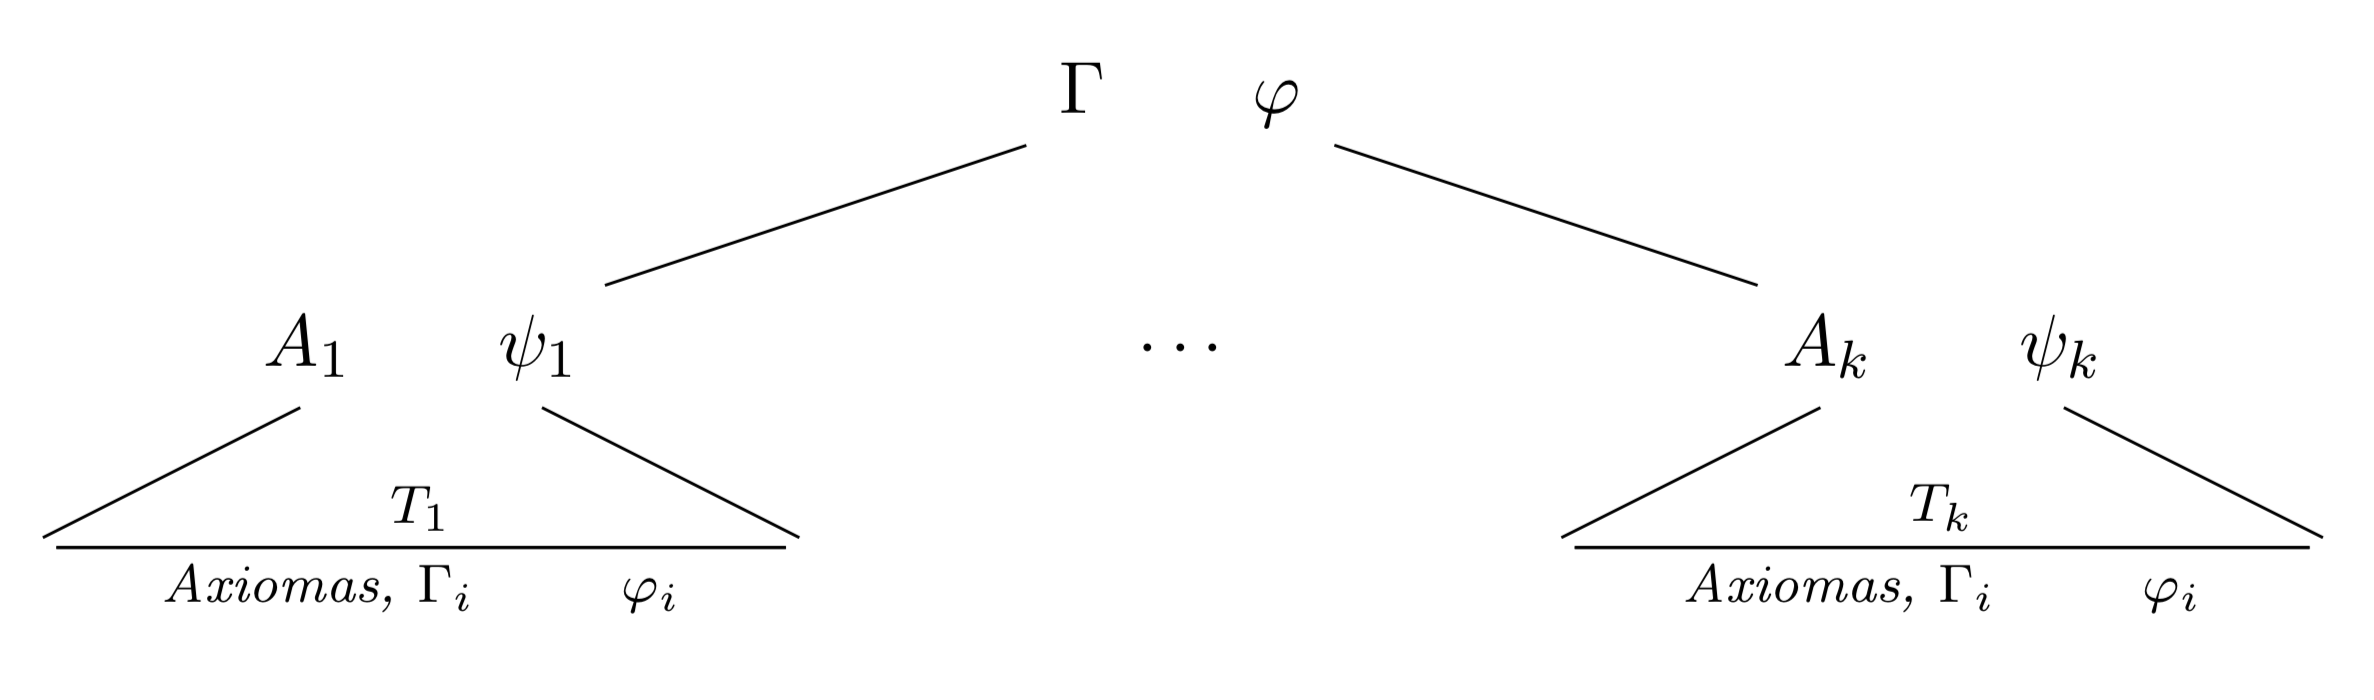
\includegraphics[scale = 0.3]{figures/arbol3.png}
\end{center}
\begin{comment}
% https://tikzcd.yichuanshen.de/#N4Igdg9gJgpgziAXAbVABwnAlgFyxMJZAZgBoAGAXVJADcBDAGwFcYkQAdDgcXoFs+9LgEdhzelC4MATmgAWWEAF9S6TLnyEUARlLbqdJq3YBBAPraRYiVzTYLy1SAzY8BImX00GLNok4cAMZQEDgIKmqumkQArHoGPsb+5gDWVuKSHHZYZimOkRruKOSkAEwJRn4g+c7qblrIpWUVvuw1LoUNACzN3pVtEbVRRcgAbL2Grf7KBjBQAObwRKAAZtIQfEglIDgQSGSTSWDMjIw0jPQARjCMAAp10f6MMCs4IDRyMBLskGBsg2sNlsaLskLpDn5jqdzlcbvdhloQM9Xu8QJ9vv5fv8nIDNohwaDED0IUgoWckbC7g8ikiXm8Pl8oD8CNjVus8QS9og4iTEGSYdcqQj2Mj6WjGcy-jVcfsQVzxrz+RTBfDOiK6aj0UzMSzpezZTsuQB2PpTJUXFXUxGizUSnVSgH6olypA8xJVAAqDgFcKt6pRDIx4F1jqBiAVhJNvJAXryPqFaqeGsD2uDDpxTp5hOJWslbFNSQCOBgAA88DhgCYS-hBHBSAACJRcXgCehmLDpGwcGTyHKKUN4qOEhW5+356NcYtl3CV6sbeh1xvN-iCdudzI9hTtmZKIA
\begin{tikzcd}
                              &                                                         &                                                                       & \Gamma\qquad\varphi \arrow[rrd, no head] \arrow[lld, no head] &                               &                                                         &                                                                       \\
                              & A_1\qquad\psi_1 \arrow[ld, no head] \arrow[rd, no head] &                                                                       & \cdots                                                        &                               & A_k\qquad\psi_k \arrow[ld, no head] \arrow[rd, no head] &                                                                       \\
{} \arrow[rr, "T_1", no head] &                                                         & {} \arrow[ll, "{\textit{Axiomas, }\Gamma_i\qquad\varphi_i}", no head] &                                                               & {} \arrow[rr, "T_k", no head] &                                                         & {} \arrow[ll, "{\textit{Axiomas, }\Gamma_i\qquad\varphi_i}", no head]
\end{tikzcd}

\end{comment}
donde 
\begin{prooftree}
\AxiomC{$A_1 \idash \psi_1$}
\AxiomC{$A_k \idash \psi_k$}
\BinaryInfC{$\Gamma \idash \varphi$}(R')
\end{prooftree}
es una regla correcta, y cada $A_l\idash\psi_l$ tiene un árbol de deducción $T_l$ de altura $<m$.\\

Como el árbol de deducción $T_l$ tiene altura $<m$, y tiene en la raíz a $A_l\idash\psi_l$ y en las hojas axiomas o elementos de $\{\Gamma_1\idash\varphi_1,\dots,\Gamma_n\idash\varphi_n\}$, por hipótesis de inducción tenemos que la regla

\begin{prooftree}
\AxiomC{$\Gamma_1 \idash \varphi_1$}
\AxiomC{$\Gamma_n \idash \varphi_n$}
\BinaryInfC{$A_l \idash \psi_l$}($R_l$)
\end{prooftree}
es correcta, para $l=1,\dots,k$.\\

De modo que si suponemos que $\Gamma_1 \idash \varphi_1$,\dots,$\Gamma_n \idash \varphi_n$ son correctas, entonces $A_l \idash \psi_l$ es correcta para $l=1,\dots,k$. Por tanto, como \regla{R'} es correcta, $\Gamma \idash \varphi$ también es correcta. Por tanto \regla{R} es correcta.
\end{itemize}
\end{proof}

\begin{cor}\label{derivcorr2}
Toda regla derivada es correcta.
\end{cor}
\begin{proof}
Directo usando \ref{bacorr} y \ref{derivcorr}.
\end{proof}
\begin{cor}\textit{(Corrección)} Si $\Phi\vdash\varphi$, entonces $\Phi\vDash\varphi$.
\end{cor}
\begin{proof}
Por definición, si $\Phi\vdash\varphi$, hay un subconjunto finito $\Gamma\subseteq\Phi$ tal que $\vdash\Gamma\idash\varphi$. Es decir, $\displaystyle\frac{}{\Gamma\idash\varphi}$ es un axioma derivado, y por \ref{derivcorr2} es correcto. De modo que se cumple $\Gamma\vDash\varphi$. Esto, a su vez, implica que $\Phi\vDash\varphi$.
\end{proof}

\section{Completitud}
Como en el caso de los \textit{tableaux} de primer orden, la completitud va a ser más complicada de demostrar que la corrección.

\begin{definition}
Decimos que un conjunto $\Phi$ es \textit{consistente}, $con(\Phi)$, si $\Phi\nvdash\bot$, es decir, no existe un subconjunto finito $\Gamma\subseteq\Phi$ tal que $\vdash\Gamma\idash\bot$.
\end{definition}

El resultado que nos llevará la gran mayoría de la sección será demostrar el teorema \ref{corsat}, que dice que si un conjunto $\Phi$ es consistente, entonces es satisfactible. Una vez demostrado este teorema, la completitud se deducirá sin mucho esfuerzo. Comenzamos con el siguiente lema:

\begin{lema}\label{regder}
Las siguientes reglas son derivadas:
\begin{enumerate}
    \item Si $\alpha$ es $\alpha$-fórmula, $$(\alpha) \frac{\Gamma, \alpha_1, \alpha_2, \alpha \idash \chi}{\Gamma, \alpha \qquad \chi}$$
    \item Si $\beta$ es $\beta$-fórmula, $$(\beta)\frac{\Gamma, \beta_1, \beta \idash \chi \quad\quad \Gamma, \beta_2, \beta \idash \chi}{\Gamma, \beta \idash \chi}$$
    \item Si $\sigma$ es $\sigma$-fórmula, $$(\sigma)\frac{\Gamma, \sigma, \sigma_1 \idash \chi}{\Gamma, \sigma \idash \chi}$$
    \item SI $\gamma$ es $\gamma$-fórmula y $t\in TERM_S$ $$(\gamma)\frac{\Gamma, \gamma(t), \gamma \idash \chi}{\Gamma, \gamma \idash \chi}$$
    \item Si $\delta$ es $\delta$-fórmula y $c\in C_A$ es nueva, $$(\delta)\frac{\Gamma, \delta(c), \delta \idash \chi}{\Gamma, \delta \idash \chi}$$
    \item Si $\theta \in EQ_S$ es $\theta$-fórmula, $$(\theta)\frac{\Gamma, \theta \idash \chi}{\Gamma \idash \chi}$$
\end{enumerate}
\end{lema}

\begin{proof} No se incluye. En cada apartado es necesario dividir en casos y crear árboles de deducción para cada caso.
\begin{comment}
No se va a hacer explícitamente. Requiere crear árboles de deducción para todas estas reglas. En los apartados 1 y 2, dada la definición  por casos de las reglas $\alpha$ y $\beta$, esto requiere 3 árboles en cada apartado. De igual forma hacen falta 3 árboles en el apartado 3, y 2 árboles en los apartados 4 y 5. El apartado 6 se divide en más casos y el caso de los axiomas $(ST_1)$ y $(ST_2)$ es más complicado y requiere argumentos inducción y la ley de sustitución generalizada.
\end{comment}
\end{proof}


\begin{prop}\label{condramas}
Sea $T$ tableau finito para $\Phi$. Sean:
$$\Gamma := \{\varphi \in \Phi \, \, | \, \, \varphi \text{ aparece en } T\}$$
$$\Gamma_r:= \{\varphi \,\, | \,\, \varphi \text{ aparece en la rama } r\}$$
Si para toda rama $r$ de $T$ se cumple que, dada la fórmula $\chi$, $\vdash \Gamma_r \idash \chi$, entonces $\vdash \Gamma \idash \chi$. 
\end{prop}
\begin{proof}
Sea $T$ \textit{tableau} finito para $\Phi$. Entonces se puede construir en un número finito de pasos $T_0, \dots, T_n$ mediante la aplicación de las reglas $R_1, \dots, R_n$.

Realizamos la demostración por inducción sobre $n$. Denotamos $\Gamma_k :=  \{\varphi \in \Phi \, \, | \, \, \varphi \text{ aparece en } T_k\}$.

Si $n = 0$ entonces tenemos un \textit{tableaux} inicial $T_0 =$
\begin{tikzcd}
\varphi_1 \arrow[d, no head]          \\
\varphi_2 \arrow[dd, no head, dotted] \\
                                      \\
\varphi_k                            
\end{tikzcd}, con $\{\varphi_1, \dots, \varphi_k\} \subseteq \Phi$. Por tanto, solo tenemos una rama $r$ que además verifica que $\Gamma = \Gamma_r$, de lo que se sigue el resultado.

Sea $n\geq 1$, supongamos que el resultado se cumple para $T_{n-1}$. Para ver que se cumple en $T_n$, tenemos que distinguir casos dependiendo de la regla que sea $R_n$. En todos los casos, usaremos la letra $r$ para nombrar las ramas de $T_{n-1}$ y $s$ para nombrar a las ramas de $T_n$.
\begin{itemize}
    \item Si $R_n = R_{\alpha}$, entonces en $T_{n-1}$ tenemos una rama $r_0$ conteniendo la $\alpha$-fórmula $\alpha$, y esa rama se extiende añadiendo $\alpha_1$ y $\alpha_2$ para formar la rama $s_0$ de $T_n$. \\
    
    Supongamos ahora que $\vdash\Gamma_s\idash\chi$ para toda rama $s$ de $T_{n}$ y queremos llegar a que se cumple $\vdash\Gamma_n\idash\chi$. Veamos primero que para toda rama $r$ en $T_{n-1}$, tenemos $\vdash\Gamma_r\idash\chi$. Para ello basta comprobar que $\vdash\Gamma_{r_0}\idash\chi$, ya que el resto de ramas $r$ que no son $r_0$ no se han extendido y son también ramas de $T_n$.\\
    
    Pero sabemos que $\vdash\Gamma_{s_0}\idash\chi$. Además, como $\alpha\in\Gamma_{r_0}$ y $\Gamma_{s_0}=\Gamma_{r_0}\cup\{\alpha_1,\alpha_2\}$, por el apartado 1 de \ref{regder} la regla $\frac{\Gamma_{s_0}\idash\chi}{\Gamma_{r_0}\idash\chi}$ es derivada. Por tanto como se cumple $\vdash\Gamma_{s_0}\idash\chi$, también se cumple $\vdash\Gamma_{r_0}\idash\chi$.\\
    
    Como tenemos $\vdash\Gamma_r\idash\chi$ para toda rama $r$ de $T_{n-1},$ por hipótesis de inducción $\vdash\Gamma_{n-1}\idash\chi$. Como $\Gamma_{n-1}\subseteq\Gamma_n$, esto implica $\vdash\Gamma_n\idash\chi$.\\
    
    \item Si $R_n = R_{\beta}$, entonces en $T_{n-1}$ tenemos una rama $r_0$ conteniendo la $\beta$-fórmula $\beta$, y esa misma rama se extiende añadiendo $\beta_1$ y $\beta_2$ para formar las ramas $s_1$ y $s_2$ de $T_n$, respectivamente. \\
    
    Supongamos ahora que $\vdash\Gamma_s\idash\chi$ para toda rama $s$ de $T_{n}$ y queremos llegar a que se cumple $\vdash\Gamma_n\idash\chi$. Veamos primero que para toda rama $r$ en $T_{n-1}$, tenemos $\vdash\Gamma_r\idash\chi$. Para ello basta comprobar que $\vdash\Gamma_{r_0}\idash\chi$, ya que el resto de ramas $r$ que no son $r_0$ no se han extendido y son también ramas de $T_n$.\\
    
    Pero sabemos que $\vdash\Gamma_{s_0}\idash\chi$. Además, como $\beta\in\Gamma_{r_0}$ y $\Gamma_{s_1}=\Gamma_{r_0}\cup\{\beta_1\}$, $\Gamma_{s_2}=\Gamma_{r_0}\cup\{\beta_2\}$ por el apartado 2 de \ref{regder} la regla $\frac{\Gamma_{s_1}\idash\chi\qquad \Gamma_{s_2}\idash\chi}{\Gamma_{r_0}\idash\chi}$ es derivada. Por tanto como se cumplen $\vdash\Gamma_{s_1}\idash\chi$ y $\vdash\Gamma_{s_2}\idash\chi$, también se cumple $\vdash\Gamma_{r_0}\idash\chi$.\\
    
    Como tenemos $\vdash\Gamma_r\idash\chi$ para toda rama $r$ de $T_{n-1},$ por hipótesis de inducción $\vdash\Gamma_{n-1}\idash\chi$. Como $\Gamma_{n-1}\subseteq\Gamma_n$, esto implica $\vdash\Gamma_n\idash\chi$.\\



    \item Si $R_n = R_{\sigma}$, entonces en $T_{n-1}$ tenemos una rama $r_0$ conteniendo la $\sigma$-fórmula $\sigma$, y esa misma rama se extiende añadiendo $\sigma_1$ para formar la rama $s_0$ de $T_n$. \\
    
    Supongamos ahora que $\vdash\Gamma_s\idash\chi$ para toda rama $s$ de $T_{n}$ y queremos llegar a que se cumple $\vdash\Gamma_n\idash\chi$. Veamos primero que para toda rama $r$ en $T_{n-1}$, tenemos $\vdash\Gamma_r\idash\chi$. Para ello basta comprobar que $\vdash\Gamma_{r_0}\idash\chi$, ya que el resto de ramas $r$ que no son $r_0$ no se han extendido y son también ramas de $T_n$.\\
    
    Pero sabemos que $\vdash\Gamma_{s_0}\idash\chi$. Además, como $\sigma\in\Gamma_{r_0}$ y $\Gamma_{s_0}=\Gamma_{r_0}\cup\{\sigma_1\}$, por el apartado 3 de \ref{regder} la regla $\frac{\Gamma_{s_0}\idash\chi}{\Gamma_{r_0}\idash\chi}$ es derivada. Por tanto como se cumple $\vdash\Gamma_{s_0}\idash\chi$, también se cumple $\vdash\Gamma_{r_0}\idash\chi$.\\
    
    Como tenemos $\vdash\Gamma_r\idash\chi$ para toda rama $r$ de $T_{n-1},$ por hipótesis de inducción $\vdash\Gamma_{n-1}\idash\chi$. Como $\Gamma_{n-1}\subseteq\Gamma_n$, esto implica $\vdash\Gamma_n\idash\chi$.\\
    
    \item Las reglas $\gamma,\delta$ siguen el mismo razonamiento que la $\sigma$ cambiando $\sigma$ por $\gamma/\delta$ y $\sigma_1$ por $\gamma(t)/\sigma(c)$ respectivamente, y usando los apartados $4/5$ de \ref{regder}.

    La regla $\theta$ también se hace de forma similar, viendo que si en la regla añadimos una fórmula $\theta$ a una rama $r_0$ de $T_{n-1}$ para obtener una rama $s_0$ de $T_n$, entonces por el apartado 6 de \ref{regder}, la regla $\frac{\Gamma_{s_0}\idash\chi}{\Gamma_{r_0}\idash\chi}$ es derivada.

    \item Si $R_n=R_{hip}$, entonces en $T_{n-1}$ tenemos una rama $r_0$, a la que añadimos la fórmula $\varphi$ de $\Phi$ para  formar la rama $s_0$ de $T_n$. \\
    
    Supongamos ahora que $\vdash\Gamma_s\idash\chi$ para toda rama $s$ de $T_{n}$ y queremos llegar a que se cumple $\vdash\Gamma_n\idash\chi$. Veamos primero que para toda rama $r$ en $T_{n-1}$, tenemos $\vdash \Gamma_r\idash \varphi\to\chi$. Dos  casos:
    \begin{itemize}
        \item $r\neq r_0$. Entonces  $r$ también es una rama de $T_n$, por tanto sabemos $\vdash\Gamma_r\idash\chi$. Por $(\mathbf{FS})$, obtenemos $\vdash\Gamma_r,\varphi\idash\chi$, y por $(\to\mathbf{C})$, llegamos a que $\vdash\Gamma_r\idash\varphi\to\chi$.
        \item $r=r_0$. Sabemos que $\vdash\Gamma_{s_0}\idash\chi$, por tanto por $(\to\mathbf{C})$, tenemos que $\vdash\Gamma_{s_0}\setminus\{\varphi\}\idash\varphi\to\chi$. Como $\Gamma_{s_0}\setminus\{\varphi\}\subseteq\Gamma_{r_0}$, por $(\mathbf{FS})$ tenemos que $\vdash\Gamma_{r_0}\idash\varphi\to\chi$.
    \end{itemize}
    De modo que como tenemos que $\vdash \Gamma_r\idash \varphi\to\chi$ para toda rama $r$ de  $T_{n-1}$, por hipótesis de inducción con la fórmula $\varphi\to\chi$ tenemos que $\vdash \Gamma_{n-1}\idash \varphi\to\chi$. Como $\Gamma_{n-1}\subseteq\Gamma_n$, tenemos $\vdash \Gamma_n\idash \varphi\to\chi$. Como además $\vdash \Gamma_n\idash \varphi$ es un axioma del supuesto, por $(\textbf{MP})$ deducimos que $\vdash \Gamma_n\idash \chi$, como queríamos.



    

\end{itemize}
\end{proof}

\begin{cor}
Si el conjunto de fórmulas $\Phi$ tiene un tableau cerrado, entonces $\Phi \vdash \bot$.
\end{cor}
\begin{proof}
Sea $T$ un \textit{tableau} cerrado para $\Phi$. Sea $r$ rama de $T$. Si $\bot \in \Gamma_r$, entonces $\vdash \Gamma_r \idash \bot$, por $\mathbf{(SP)}$. Si existe cierta $\varphi$ tal que $\varphi, \neg\varphi\in \Gamma_r$, entonces, por $\mathbf{(CT_2)}$, $\vdash \Gamma_r \idash \bot$. 

De modo que como para cada rama $r$ se cumple $\vdash \Gamma_r \idash \bot$, por \ref{condramas} tenemos $\vdash \Gamma \idash \bot$, con $\Gamma := \{\varphi\in \Phi \, \, | \, \, \varphi \text{ está en } T\}$. Como $\Gamma$ es subconjunto finito de $\Phi$, $\Phi \vdash \bot$.
\end{proof}



\begin{theorem}\label{corsat}
Si $con(\Phi)$, entonces $Sat(\Phi)$.
\end{theorem}
\begin{proof}
Es la forma contrarrecíproca del resultado anterior.
\end{proof}

\begin{cor}(Completitud)
Si $\Phi \vDash \varphi$, entonces $\Phi \vdash \varphi$.
\end{cor}
\begin{proof}
Si $\Phi \vDash \varphi$ entonces $Insat(\Phi \cup \{\neg \varphi\})$, es decir, por \ref{corsat} es falso que $con(\Phi\cup \{\neg \varphi\})$, y entonces existe un subconjunto finito $\Gamma\subseteq\Phi\cup \{\neg \varphi\}$ tal que $\vdash\Gamma\idash\bot$.
Tenemos, por tanto, 
\begin{center}
    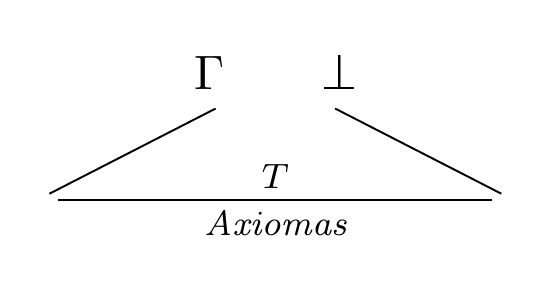
\includegraphics[scale = 0.3]{figures/arbol4.png}
\end{center}
Veamos si existe un subconjunto finito $\Delta \subseteq \Phi$ tal que $\vdash\Delta\idash\bot$.
\begin{itemize}
    \item Si $\neg \varphi \notin \Gamma$, tomando $\Delta := \Gamma$ obtenemos:
\begin{center}
    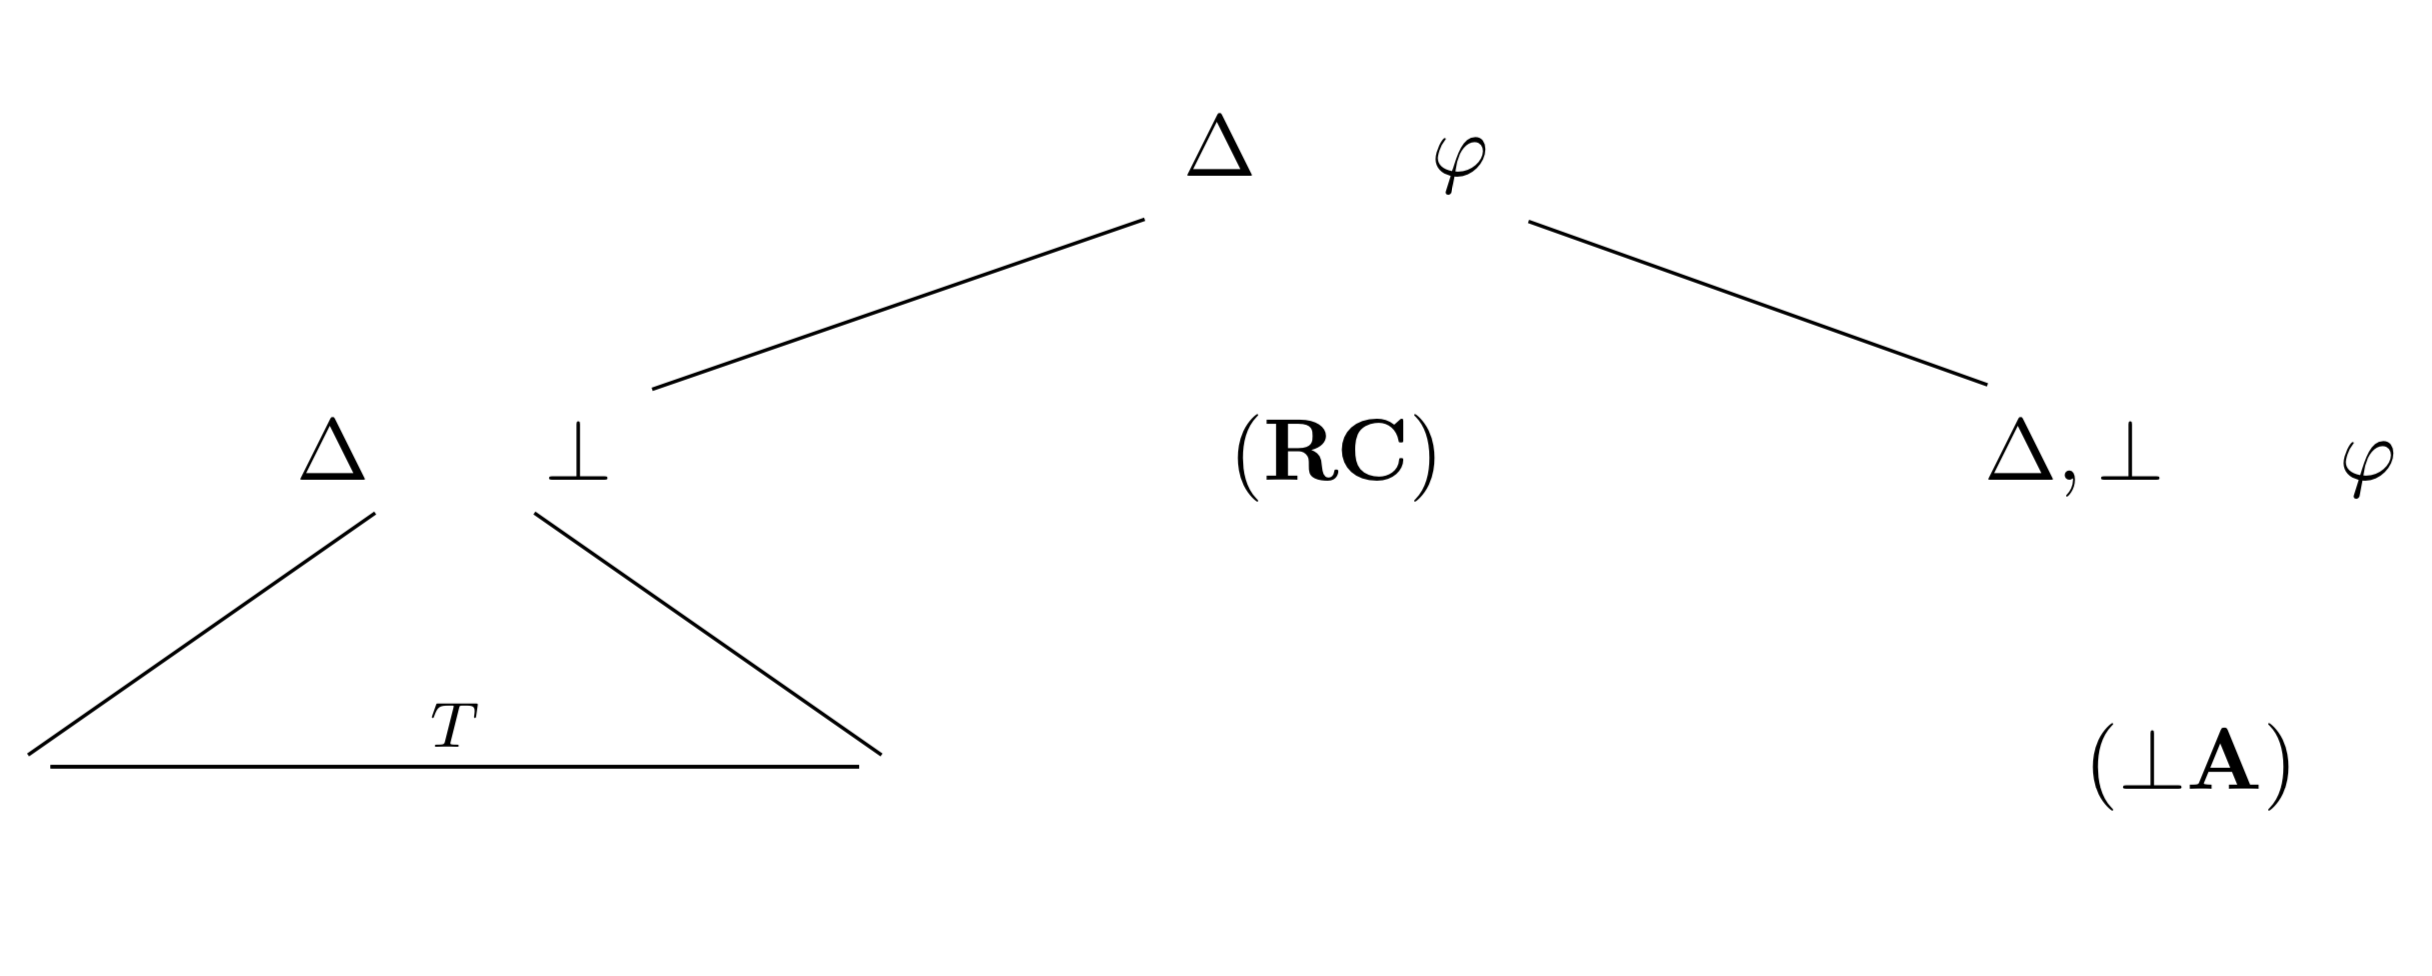
\includegraphics[scale = 0.25]{figures/arbol5.png}
\end{center}
\begin{comment}
% https://tikzcd.yichuanshen.de/#N4Igdg9gJgpgziAXAbVABwnAlgFyxMJZAZgBoAGAXVJADcBDAGwFcYkQAdDgcXoFs+9LgEdhzelC4MATmgAWWEAF9S6TLnyEUARlLbqdJq3ZdeA+gAIRYiVY4AjCDmWqQGbHgJEy+mgxZsiCAAFFw4MAAeOPYAZsAASgDCSgCULmoemkQArHoG-sZBpvyCpHaOOHai4lB2MvKKKhkaXijkpABM+UaBIOlu6p5ayB2d3QHs-e4tw7ldfj3soQ5OXII4crHAAIKpygYwUADm8ESgMdIQfEjtIDgQSGSGE4hgzIyMNIz09jCMAAqDLJBRgwGLOGhyGASdiQMBsJogC5XG40e5IXTPQpvD5fH5-QGZVogUHgkCQ6FQWEEBGuZHXRCY9GIAAsCxeOM+JPxAKBxNJEJAUJhQThtPOlwZTIeiFyWMCnLxv15RK0JLBguFVNFNP69KQbLuMrlBV6ABVydzlYSZuwBZatdT4XrJUg5czDaakIqrQS+Wr7RSReBdUpKEogA
\begin{tikzcd}
                            &                                                            &                        & \Gamma\qquad\varphi \arrow[rrd, no head] \arrow[lld, no head] &  &                               \\
                            & \Gamma \qquad \bot \arrow[ld, no head] \arrow[rd, no head] &                        & (\textbf{RC})                                                 &  & {\Gamma, \bot \qquad \varphi} \\
{} \arrow[rr, "T", no head] &                                                            & {} \arrow[ll, no head] &                                                               &  & (\bot\mathbf{A})             
\end{tikzcd}
\end{comment}

    \item Si $\neg \varphi \in \Delta$, tomando $\Delta := \Gamma \setminus \{\neg \varphi\}$ obtenemos:
\begin{center}
    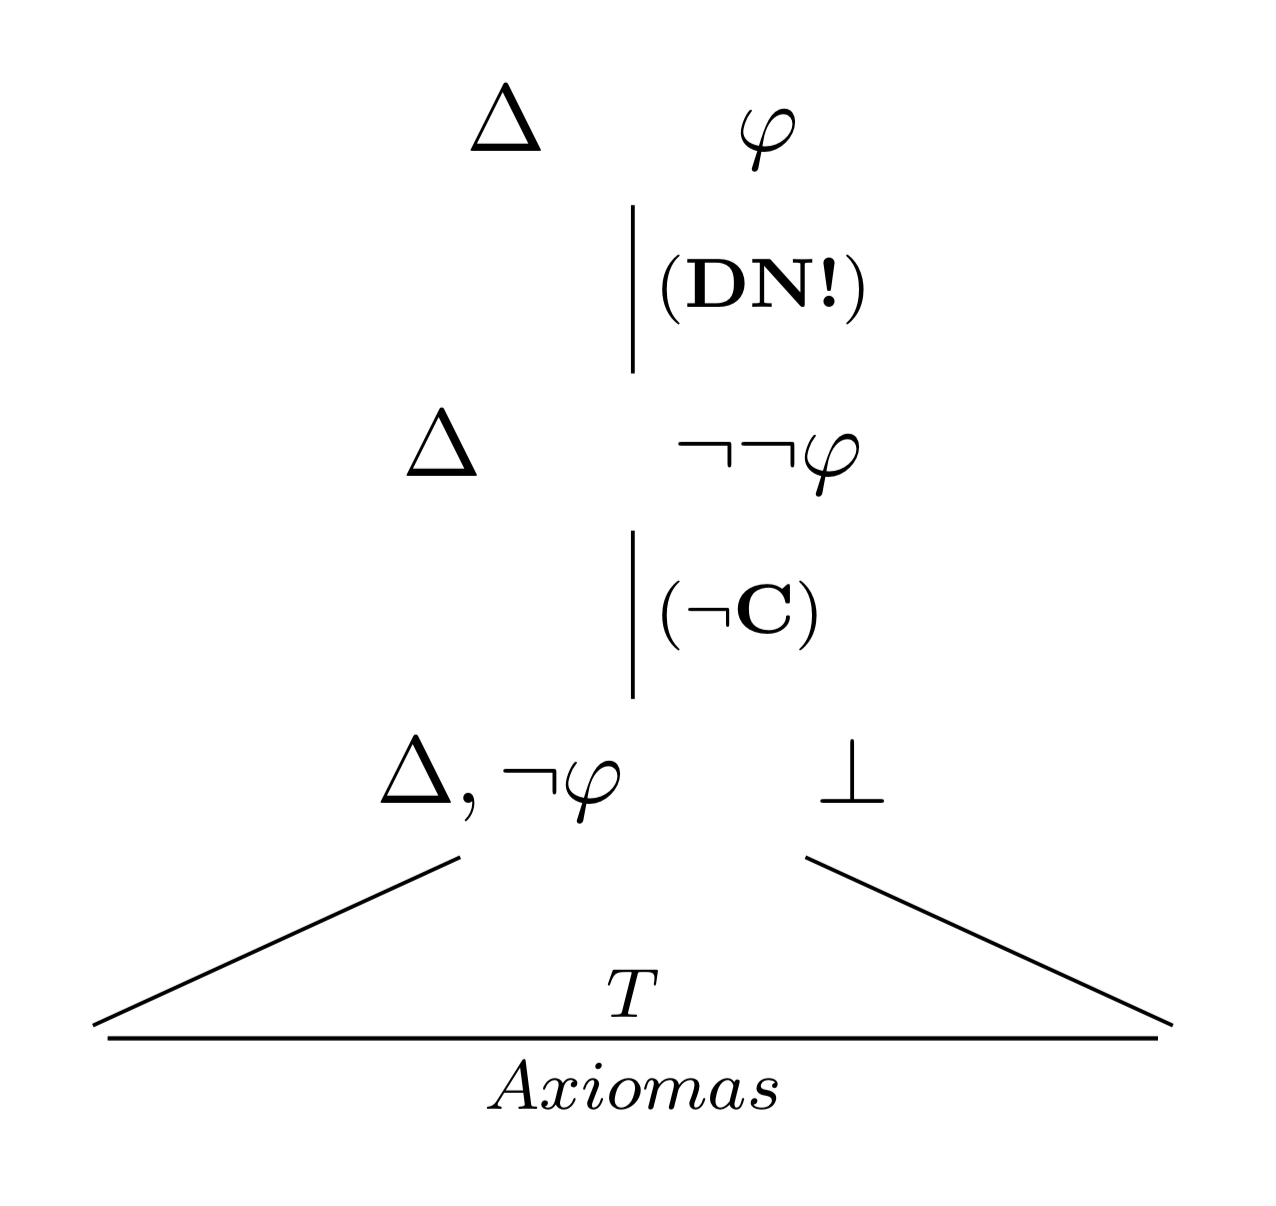
\includegraphics[scale = 0.23]{figures/arbol6.png}
\end{center} 
\begin{comment}
% https://tikzcd.yichuanshen.de/#N4Igdg9gJgpgziAXAbVABwnAlgFyxMJZARgBoAmAXVJADcBDAGwFcYkQAdDgERkZ3qkABFzAwA5lwYAnNAAssXAI5Lm9KFwBGEHCAC+pdJlz5CKAAykAzNTpNW7fYZAZseAkXLXbDFm0QgTkZupkRkxD72-pw8fAIiHCpqUAlikhxpUvSyCkEuxu5mJKTmkX7sXLz89AlJ6gky8lhC+rYwUOLwRKAAZtIQALZIliA4EEhkduWIYMyMjDSM9Jp8AAoFoQGMMD26NHIw6uyQYnl9g8M0Y0heUw4zcwsgSyuM6yEeWzt7IAdHASc2AZev0hohJtdELdfPcQAAVECLZZrDafZ7fRG-Q5QY4EIHOc5g26QyZ-HEAvGYmHRACCAA98AN6AhgSBCZdRuNEFZ9tjcacka93iY0dIsOI5D9qewABSiCRcHAwOk4TQ9YAAYT0AEozqCkDzOUgACy8-7gSmClEfMwgMUSqVRWWK5Wq9XcAByAEIda09EA
\begin{tikzcd}
                            & \Delta \qquad \varphi                                                                                           &                                   \\
                            & \Delta \qquad \neg\neg\varphi \arrow[u, "(\textbf{DN!})"', no head]                                             &                                   \\
                            & {\Delta, \neg\varphi\qquad\bot} \arrow[ld, no head] \arrow[rd, no head] \arrow[u, "(\neg\textbf{C})"', no head] &                                   \\
{} \arrow[rr, "T", no head] &                                                                                                                 & {} \arrow[ll, "Axiomas", no head]
\end{tikzcd}
\end{comment}
\end{itemize}
de modo que en ambos casos se cumple el enunciado.
\end{proof}

De modo que hemos visto que si $S$ es signatura numerable y $\Phi \subseteq FORM_S$ es insatisfactible, entonces $\Phi$ tiene \textit{tableau} cerrado y es, por tanto, inconsistente. De hecho, este resultado también se puede demostrar cuando $S$ no es numerable.\footnote{Este resultado se puede encontrar en el capítulo 5 del libro \textit{Mathematical Logic}, de los autores H.-D. Ebbinghaus, J. Flum y W. Thomas.}\\


Finalmente, demos una visión global de lo que hemos estudiado en estas últimas subsecciones. Partiendo de los dos pares de conceptos \textit{deducción formal}-\textit{consistencia}  y \textit{corrección}-\textit{satisfactibilidad} hemos establecido un nexo entre las perspectivas sintáctica y semántica, respectivamente representadas por cada par de tales conceptos. \\

Este nexo consiste en los Teoremas de Corrección y Completitud, que nos permiten pasar `de un lado a otro': El teorema de corrección nos permite traducir algunas afirmaciones sintácticas a semánticas, y el de completitud nos permite traducir afirmaciones semánticas a sintácticas.\\

A continuación mostramos la correspondencia que hemos definido:
\begin{align*}
    \text{\large Sintaxis} & \qquad  \text{\large Semántica} \\   
    \text{Fórmulas} & \Longleftrightarrow  \text{ Modelos} \\
    \Phi \vdash \varphi \quad (\Phi \vdash_{tb} \varphi) & \Longleftrightarrow  \Phi \vDash \varphi \\
    con(\Phi) & \Longleftrightarrow sat(\Phi) \\
    \vdash \varphi \leftrightarrow \psi & \Longleftrightarrow \varphi \sim \psi \\
    \vdash \varphi & \Longleftrightarrow \vDash \varphi
\end{align*}

\chapter{Alcance y limitaciones de la lógica de primer orden}


Vamos a dedicar esta sección a estudiar las nociones y resultados más importantes de este manual.


\section{Teorema de Compacidad y modelos}

Comencemos demostrando una versión más general de \ref{compacidad}, que se convertirá en una de nuestras herramientas básicas en las siguientes secciones: 

\begin{theorem}\label{comp2} (Teorema de compacidad)
Sea $S$ signatura, $\Phi\subseteq PROP_S$, $\varphi\in PROP_S$. Entonces,
\begin{enumerate}[label=\alph*)]
    \item $\Phi\vDash\varphi$ si y solo si existe $\Phi_0\subseteq_{fin}\Phi$ tal que $\Phi_0\vDash\varphi$.
    \item $sat(\Phi)$ si y solo si para todo $\Phi_0\subseteq_{fin}\Phi$, se cumple $sat(\Phi_0)$.
\end{enumerate}
\end{theorem}

\begin{proof}
Demostramos solo el caso de signatura $S$ numerable, que es donde hemos estudiado los teoremas de corrección y completitud. El caso no numerable también se puede demostrar.\footnote{Una prueba se puede encontrar en \textit{Logic and Structure}, Dirk Van Dalen, Ed. Springer}
\begin{enumerate}[label=\alph*)]

\item  La implicación $\Longleftarrow$ es trivial. Veamos $\Longrightarrow$. Si $\Phi\vDash\varphi$, $\Phi\vdash\varphi$, por tanto hay $\Phi_0\subseteq\Phi$ finito tal que $\vdash\Phi_0\idash\varphi$, de modo que $\Phi_0\vdash\varphi$ y por tanto $\Phi_0\vDash\varphi$.

\item  La implicación $\Longrightarrow$ es trivial. Veamos $\Longleftarrow$ en su forma contrapositiva. Si $insat(\Phi)$, $\Phi\vdash\bot$, por tanto hay $\Phi_0\subseteq\Phi$ finito tal que $\vdash\Phi_0\idash\bot$, luego $\Phi_0\vdash\bot$ y por tanto $\Phi_0\vDash\bot$, es decir, $Insat(\Phi_0)$.
\end{enumerate}
\end{proof}



Recordemos que una sentencia es una fórmula de primer orden en que ninguna variable aparece libre. Pues bien, a partir de ahora vamos a trabajar con sentencias. Dada una signatura $S$, definimos $Sent_S:=\{\varphi\in FORM_S\, \, |\, \, lib(\varphi)=\emptyset\}$.\\

Ahora supongamos que tenemos una signatura $S$, una $S$-álgebra $\mathfrak{A}$ con conjunto soporte $A$ y una sentencia $\varphi\in Sent_S$, y sean $\sigma_1,\sigma_2: Var \rightarrow A$ funciones que asignan valores a las variables. Con ellas podemos definir dos interpretaciones, $\mathfrak{I}_1 := \langle \mathfrak{A}, \sigma_1 \rangle$ y , $\mathfrak{I}_2 := \langle \mathfrak{A}, \sigma_2 \rangle$. Entonces, por el Lema de Coincidencia \ref{coinc}, como $lib(\varphi)=\emptyset$, tenemos que $\varphi^{\mathfrak{I}_1}=\varphi^{\mathfrak{I}_2}$.\\

Es decir, que una interpretación $\mathfrak{I} := \langle \mathfrak{A}, \sigma \rangle$ verifique o no una sentencia solo depende de $\mathfrak{A}$, no de $\sigma$. Por tanto, es natural introducir la siguiente definición:

\begin{definition}
Dadas una signatura $S$, una $S$-álgebra $\mathfrak{A}$ y una sentencia $\varphi\in Sent_S$, decimos que $\mathfrak{A}\vDash\varphi$, $\mathfrak{A}$\textit{ es un modelo de $\varphi$}, cuando para alguna asignación $\sigma : Var \rightarrow A$ la $S$-interpretación $\mathfrak{I} := \langle \mathfrak{A}, \sigma \rangle$ verifica $\varphi$.
\end{definition}

\begin{definition}
Si $\Phi\subseteq Sent_S$, definimos la siguiente clase:
\[Mod_S(\Phi)=\{\mathfrak{A}\, \, |\, \, \mathfrak{A} \text{ \textit{S}-álgebra y }\mathfrak{A}\vDash\varphi \text{ para toda $\varphi\in\Phi$}\}.\]
Así, decimos que una álgebra $\mathfrak{A}$ es modelo de $\Phi$ si $\mathfrak{A}\vDash\varphi \text{ para toda $\varphi\in\Phi$}$. \\
\end{definition}

\begin{theorem}\label{fintoinf}
Si $\Phi\subseteq Sent_S$ admite modelos finitos arbitrariamente grandes, entonces admite algún modelo infinito.
\end{theorem}

\begin{proof}
Para cada $n$, tenemos un modelo $\mathfrak{A_n}$ de soporte $A_n$ con $|A_n|>n$.
Ahora vamos a definir para cada $n\geq2$ una sentencia $\varphi_n$ que dice `hay al menos $n$ elementos en el conjunto soporte':\\
$\varphi_2=\exists x\exists y\neg x\doteq y$\\
$\varphi_3=\exists x\exists y\exists z\neg x\doteq y\land\neg x\doteq z\land\neg y\doteq z$\\
$\vdots$\\
$\varphi_n=\exists x_1\exists x_2\dots\exists x_n\bigwedge_{i=1}^n\bigwedge_{j=i+1}^n\neg x_i\doteq x_j$\\
$\vdots$\\

No es difícil verificar que una estructura es modelo de $\varphi_n$ si y solo si su soporte tiene al menos $n$ elementos.
Ahora definimos el conjunto de sentencias $\hat{\Phi}:=\Phi\cup\{\varphi_n\}_{n\geq2}$.
Si comprobamos que $\hat{\Phi}$ es satisfactible habremos acabado, ya que cualquier modelo de $\hat{\Phi}$ tiene que tener infinitos elementos en su soporte. Pero por el Teorema de Compacidad, para esto nos basta comprobar que cualquier subconjunto finito de $\hat{\Phi}$ es satisfactible.

Sea $\Phi_0\subseteq\hat{\Phi}$ finito. Entonces podemos definir $n_0:=\max\{n\in\mathbb{N}|\varphi_n\in\Phi_0\}$. Y está claro que $\mathfrak{A}_{n_0}$ es modelo de $\Phi_0$, ya que es modelo de $\Phi$ y de $\varphi_n$ para cualquier $n\leq n_0$. Por tanto $\Phi_0$ es satisfactible.
\end{proof}

\section{Teoremas de Löwenheim-Skolem}

Nos disponemos ahora a ver los teoremas de Löwenheim-Skolem que, dado un conjunto de sentencias $\Phi$, nos garantizan la existencia de modelos para $\Phi$ de cardinales grandes (versión ascendente del teorema) o pequeños (versión descendente del teorema). En los siguientes teoremas, con el `cardinal de una signatura' nos referimos al cardinal del conjunto de constantes, funciones y predicados de la signatura, y con el `cardinal de un modelo' nos referimos al cardinal de su conjunto soporte.

\begin{theorem}
(Teorema de Löwenheim-Skolem, caso numerable descendente)\\
Sea $S$ signatura numerable, $\Phi\subseteq Sent_S$ satisfactible. Entonces $\Phi$ tiene un modelo a lo sumo numerable.
\end{theorem}
\begin{proof}
Como $S$ es numerable y $\Phi$ es satisfactible, el \textit{tableau} canónico para $\Phi$ tendrá alguna rama abierta $r$, de modo que $\Phi\subseteq\Gamma_r$ y $\Gamma_r$ es de Hintikka. Entonces cogemos la interpretación $\mathfrak{I}_{\Gamma_r}$, como está definida en \ref{Hinti33}.\\

Esta interpretación satisface $\Gamma_r$, de modo que como $\Phi\subseteq\Gamma_r$, también satisface $\Phi$. Es decir, su álgebra $\mathfrak{T}_{\Gamma_r}$ es modelo de $\Phi$.

Además, su conjunto soporte es $T_{\Gamma_r}/\equiv_{\Gamma_r}$. Pero $\abs{T_{\Gamma_r}/\equiv_{\Gamma_r}}\leq|T_{\Gamma_r}|\leq|FORM_S|$. Como $FORM_S$ es numerable, este es el modelo con soporte numerable que buscábamos.
\end{proof}

Pasamos a ver la versión general del teorema anterior, de la cual no se incluye demostración.

\begin{theorem}\label{LSD} (Teorema de Löwenheim-Skolem descendente)\\
Sea $S$ signatura, $\Phi\subseteq Sent_S$ satisfactible. Entonces $\Phi$ tiene un modelo de cardinal $\leq|FORM_S|$.
\end{theorem}

\begin{note}
Para cada signatura con conjunto de símbolos de constante $C$, podemos considerar el conjunto de fórmulas que nos dicen que las constantes son distintas dos a dos, $\Phi_C=\{\neg c_1\doteq c_2\}_{c_1,c_2\in C;c_1\neq c_2}$. Entonces, cualquier modelo de $\Phi$ tiene que tener cardinal $\geq |C|$.

Esto nos dice que el teorema \ref{LSD} no es mejorable:

Supongamos que tenemos una signatura $S$ sin funciones ni predicados y con un conjunto infinito $C$ de constantes. Entonces, se puede comprobar que $|FORM_S|=|C|$. Si ahora consideramos el conjunto de sentencias $\Phi_C$, es satisfactible (basta elegir un modelo $\mathfrak{A}$ cuyo conjunto  soporte sea el propio conjunto de constantes y definir $c^\mathfrak{A}=c$ para toda constante $c$), sin embargo, cualquier  modelo de $\Phi_C$ tiene cardinal superior a $|C|=|FORM_S|$. De modo que en este caso, la desigualdad de \ref{LSD} no puede  ser  estricta.
\end{note}

\begin{example}
Sea la signatura $S=\langle0,1,\cdot,+,<\rangle$ y el álgebra habitual de los reales, $\mathbb{R}^<=\langle\mathbb{R};0,1;\cdot,+;\leq\rangle$.\\

Entonces podemos definir el conjunto de sentencias que cumple $\mathbb{R}^<$:

\[Th(\mathbb{R}^<) :=\{\varphi\in Sent_S\, \, | \, \, \mathbb{R}^<\vDash\varphi\})\]

El teorema \ref{LSD} nos dice que de hecho hay un modelo numerable $\mathbb{R}^!$ que también verifica $Th(\mathbb{R}^<)$, es decir, cualquier sentencia que cumpla $\mathbb{R}^<$ también la cumple este modelo numerable $\mathbb{R}^!$.
\end{example}

Pasamos directamente a ver la versión ascendente del Teorema de Löwenheim-Skolem, que sí podremos demostrar (usando el caso no numerable del teorema de compacidad).

\begin{theorem}(Teorema de Löwenheim-Skolem ascendente)
Sea $S$ signatura, $\Phi\subseteq Sent_S$ de forma que existe algún modelo infinito de $\Phi$, y sea $\kappa$ un cardinal. Entonces $\Phi$ tiene un modelo de cardinal $\geq\kappa$.
\end{theorem}

\begin{proof}
Sea $K$ un conjunto de cardinal $\kappa$ (por ejemplo, $K=\kappa$). Consideramos una nueva signatura que resulta de añadir a $S$ una constante por cada elemento de $K$:
\[S'=S\cup\{c_a;a\in K\}\qquad\text{donde $c_a\neq c_b$ si $a\neq b$.}\]
Sea $\Phi'\subseteq FORM_{S'}$ definido como $\Phi\cup\{\neg c_a\doteq c_b|a,b\in K,a\neq b\}$. Veamos primero que $\Phi'$ es satisfactible. Para ello, claro, nos basta el teorema de compacidad \ref{comp2}.

De modo que sea $\Phi_0\subseteq\Phi'$ finito, veamos que es satisfactible. Sean $a_1,\dots,a_k$ los elementos $a$ de $K$ tales que $c_a$ aparece en alguna fórmula de $\Phi_0$. Entonces, llamando $\Phi_1=\Phi\cup\{\neg c_{a_i}\doteq c_{a_j}|i,j\in\{1,\dots,n\},i\neq j\}$, tenemos que $\Phi_0\subseteq\Phi_1$.\\

Pero $\Phi_1$ es satisfactible, ya que como $\Phi$ tiene un modelo infinito $\mathfrak{A}$ en $S$, podemos elegir el modelo $\mathfrak{A}$ para $\Phi_1$ en $S'$, asignando $k$ elementos distintos del conjunto soporte a $c_{a_1},\dots,c_{a_k}$ y asignando los valores que queramos al resto de constantes.\\

Por tanto, por el Teorema de Compacidad, ya tenemos que $\Phi'$ es satisfactible en la signatura $S'$. Sea $\mathfrak{A}_0$ una $S'$-álgebra que satisface $\Phi'$. Entonces, el cardinal de $\mathfrak{A}_0$ es $\geq\kappa$, ya que tenemos $\kappa$ constantes distintas y $\Phi'$ afirma que representan distintos elementos del conjunto soporte. Hemos encontrado una $S'$-álgebra que satisface $\Phi$ de cardinal $\geq\kappa$. Para probar el enunciado, queremos una $S$-álgebra que cumpla lo mismo.\\

Para ello basta definir la $S$-álgebra $\mathfrak{A}_1$, que tiene el mismo soporte que $\mathfrak{A}_0$ y asigna a cada constante, función y predicado de $S$ lo mismo que $\mathfrak{A}_0$. Como $\mathfrak{A}_0$ es modelo de $\Phi$, $\mathfrak{A}_1$ también será modelo de $\Phi$. Por tanto, ya hemos encontrado una $S-$álgebra que satisface $\Phi$, y de cardinal $\geq\kappa$, como queríamos.
\end{proof}

\begin{theorem}(Teorema de Löwenheim-Skolem-Tarski)\label{LST} Sean $S$ signatura, $\Phi \subseteq Sent_S$ con modelos infinitos y $\kappa$ cardinal tal que $\kappa \geq |FORM_S|$. Entonces existe $\mathfrak{A} \in Mod(\Phi)$ tal que $|\mathfrak{A}| = \kappa$.
\end{theorem}
\begin{proof}
Usando la misma notación que en el teorema anterior, podemos obtener una $S'$-álgebra de cardinal $\kappa$ que consiste en añadir constantes a $\Phi$ y un conjunto de sentencias $\Phi'\subseteq FORM_{S'}$ satisfactible y tal que cualquier modelo de $\Phi'$ tiene cardinal $\geq\kappa$.\\

Pero entonces, por el Teorema de Löwenheim descendente, \ref{LSD}, tenemos que hay una $S'$-álgebra $\mathfrak{A}$ que satisface $\Phi'$ y de cardinal $\leq\kappa$. Como es modelo de $\Phi'$, tiene cardinal $\geq\kappa$, por tanto $\mathfrak{A}$ tiene  cardinal exactamente $\kappa$.\\

Ahora, igual que en el teorema anterior, creamos una $S$-álgebra $\mathfrak{A}_1$ con el mismo conjunto soporte que $\mathfrak{A}$ y que asigna a cada constante, función y predicado de $S$ lo mismo que $\mathfrak{A}$. $\mathfrak{A}_1$ es un modelo de $\Phi$ de cardinal $\kappa$, como queríamos.
\end{proof}

\section{Axiomatizabilidad}


\begin{defs}
Dada $S$ signatura, sea $\mathcal{K}$ clase de $S$-álgebras.
\mbox{}
\begin{itemize}
    \item $\mathcal{K}$ se dice \textit{clase elemental (o finitamente axiomatizable)} si existe $\Phi \subseteq Sent_S$ finito tal que $\mathcal{K} = Mod(\Phi)$.
    \item $\mathcal{K}$ se dice \textit{clase} $\Delta$-\textit{elemental (o axiomatizable)} si existe $\Phi \subseteq Sent_S$ tal que $\mathcal{K} = Mod(\Phi)$.
\end{itemize}
\end{defs}

\begin{example}
Sea $G := \langle \cdot, e \rangle$. Sea 
\[
    \Phi_G := \Bigg\{\begin{array}{lr}
       \forall x \forall y \forall z \, (x \cdot(y\cdot z))= ((x \cdot y) \cdot z)\\
       \forall x \, x\cdot e \doteq x\land e \cdot x \doteq x\\
        \forall x \exists y \, x\cdot y \doteq e \land y\cdot x \doteq e
        \end{array} 
\]
Sea $\mathcal{K}:=\{\mathfrak{A} \, \, | \, \, \mathfrak{A} \text{ es grupo}\}$. Entonces es claro que $\mathcal{K} = Mod(\Phi_G)$, por tanto $\mathcal{K}$ es elemental.
\end{example}

\begin{example}
Sea $C := \langle 0, 1, +|_2, \cdot|_2\rangle$ y sea $\Phi_C$ el conjunto de las sentencias que expresan los axiomas de cuerpos. Si queremos expresar la propiedad de `ser de característica 0' necesitamos las sentencias $\Phi_C \cup \{\neg \chi_p \, \, | \, \, p \text{ es primo}\}$, siendo $$\chi_{p} := 1  \underbrace{+ \cdots +}_\text{$p$ veces} 1 \doteq 0.$$ Por tanto, solo podemos afirmar que $\mathcal{K}:=\{\mathfrak{A} \, \, | \, \, \mathfrak{A} \text{ es cuerpo de característica 0}\}$ es $\Delta$-elemental. De hecho, veremos que no es elemental.
\end{example}

\begin{example}
$\mathcal{K} := \{\mathfrak{A} \, \, | \, \, \mathfrak{A} \text{ es cuerpo algebraicamente cerrado}\}$ es clase $\Delta$-elemental.
\end{example}


Conviene hacer notar lo siguiente. Dada $S$ signatura, dada la clase elemental $\mathcal{K}$ y el conjunto finito $\Phi := \{\varphi_1, \dots, \varphi_n\}\subseteq Sent_S$ tal que $\mathcal{K} = Mod(\Phi)$, sea $\varphi := \varphi_1  \land \dots \land \varphi_n$. Entonces $A \in Mod(\Phi)$ si y solo si $A \in Mod(\varphi)$. Por tanto, hemos probado que

\begin{prop}
Dada $S$ signatura, la clase de $S$-estructuras $\mathcal{K}$ es elemental si y solo si existe $\varphi \in Sent_S$ tal que $\mathcal{K} = Mod(\varphi)$.
\end{prop}

\begin{prop}\label{finitaxio}
Sea $S$ signatura. \mbox{}
\begin{enumerate}
    \item Si $\mathcal{K}$ es elemental y existe $\Phi \subseteq Sent_S$ tal que $Mod(\Phi) = \mathcal{K}$, entonces existe $\Phi_0 \subseteq \Phi$ finito tal que $Mod(\Phi_0) = \mathcal{K}$.
    \item $\mathcal{K}$ es elemental si y solo si $\mathcal{K}$ y $\mathcal{K}^{\complement}$ son $\Delta$-elementales.
\end{enumerate}
\end{prop}
\begin{proof}\mbox{}
\begin{itemize}
    \item[(1)] Si $\mathcal{K}$ es elemental, existe $\varphi \in Sent_S$ tal que $\mathcal{K} = Mod(\varphi)$. Como, por otro lado, $\mathcal{K} = Mod(\Phi)$, $\Phi \vDash \varphi$ y, por compacidad, existe $\Phi_0 \subseteq \Phi$ finito tal que $\Phi_0 \vDash \varphi$, luego $$\mathcal{K} = Mod(\varphi) \subseteq Mod(\Phi_0) \subseteq Mod(\Phi)= \mathcal{K},$$ con lo que $\mathcal{K} = Mod(\Phi_0)$.
    \item[(2)] Si $\mathcal{K}$ es elemental, es claramente $\Delta$-elemental y, además, existe $\varphi \in Sent_S$ tal que $\mathcal{K} = Mod(\varphi)$, con lo que $Mod(\neg \varphi) = \mathcal{K}^{\complement}$, lo que nos da que $\mathcal{K}^{\complement}$ es elemental y por tanto $\Delta$-elemental. 
    
    Recíprocamente, si $\mathcal{K}$ y $\mathcal{K}^{\complement}$ son $\Delta$-elementales, entonces existen $\Phi, \Psi \subseteq Sent_S$ tales que $$Mod(\Phi) = \mathcal{K} \text{ y } Mod(\Psi) = \mathcal{K}^{\complement}$$
    Vemos que $Mod(\Phi \cup \Psi) = Mod(\Phi) \cap Mod(\Psi) = \mathcal{K} \cap \mathcal{K}^{\complement} = \emptyset$, con lo que $\Phi \cup \Psi$ es insatisfactible. Por compacidad, existe un subconjunto finito de $\Phi \cup \Psi$ de la forma $\Phi_0 \cup \Psi_0$, con $\Phi_0 \subseteq \Phi$ y $\Psi_0 \subseteq \Psi$ finitos, que es insatisfactible, esto es, $Mod(\Phi_0 \cup \Psi_0) = \emptyset$. Por otro lado, 
    $$\mathcal{K} = Mod(\Phi) \subseteq Mod(\Phi_0) \text{ y } \mathcal{K}^{\complement} = Mod(\Psi) \subseteq Mod(\Psi_0).$$
    Esto junto a que $Mod(\Phi_0)\cap Mod(\Psi_0)=\emptyset$ nos permite deducir que $Mod(\Phi_0)\cap\mathcal{K}^{\complement}=\emptyset$, es decir, $Mod(\Phi_0)\subseteq\mathcal{K}$. Por tanto $Mod(\Phi_0)=\mathcal{K}$, lo cual conlleva que $\mathcal{K}$ es elemental, como queríamos ver.
\end{itemize}
\end{proof}

\begin{example}
Consideremos de nuevo la signatura $C$, los axiomas de cuerpos, $\Phi_C$, y las fórmulas $\chi_p$, $p \in \N$. Definamos $\Psi := \Phi_C \cup \{\neg\chi_p \, \, | \, \, p\in \N \}$ y $\mathcal{K} :=\{\mathfrak{A} \, \, | \, \, \mathfrak{A} \text{ es cuerpo de característica 0}\}$. Ya vimos que $\mathcal{K} = Mod(\Psi)$ y, por tanto, que $\mathcal{K}$ es clase $\Delta$-elemental. Veamos que no es finitamente axiomatizable.\\

Si fuera finitamente axiomatizable, por \ref{finitaxio} existiría cierto $\Psi_0 \subseteq \Psi$ finito tal que $\mathcal{K} = Mod(\Psi_0)$. Por ser finito, existe $p$ primo tal que $\Psi_0 \subseteq \Phi_p := \Phi_C \cup \{\neg\chi_q \, \, | \, \, q \leq p \}$. Consideremos el cuerpo $\F_t$ de $t$ elementos, con $t > p$ primo. Este cuerpo no es de característica 0 y satisface $\Phi_p$, lo que contradice la suposición de que $\mathcal{K} = Mod(\Psi_0)$.
\end{example}


\begin{example}
En las condiciones anteriores se puede demostrar, por compacidad, que si $\Psi \vDash \sigma$, con $\sigma \in Sent_C$, entonces $\sigma$ es satisfactible en todos los cuerpos de característica mayor que $p$, para cierto primo suficientemente grande.

De aquí se sigue que, si $f, g \in \Z[x]$ son coprimos en $\Q[x]$, entonces son coprimos en $\Z_p[x]$, para cierto primo $p$ suficientemente grande.
\end{example}

\begin{defs}
\begin{itemize}\mbox{}
    \item Sea $S$ una signatura, $\mathfrak{A}$ una $S$-álgebra. Definimos \textit{la teoría de} $\mathfrak{A}$ como:
$$Th(\mathfrak{A}) := \{\sigma \in Sent_S \, \, | \, \, \mathfrak{A}\vDash \sigma\}$$
    \item Dos $S$-álgebras $\mathfrak{A}, \mathfrak{B}$ se dicen \textit{elementalmente equivalentes}, $\mathfraq{A} \equiv \mathfrak{B}$ si $Th(\mathfrak{A}) = Th(\mathfrak{B})$.
\end{itemize}
\end{defs}

\begin{prop}\label{equiso}
Sea $S$ signatura y sean $\mathfrak{A}, \mathfrak{B}$ dos $S$-álgebras. Si $\mathfrak{A} \approx \mathfrak{B}$, entonces $\mathfrak{A} \equiv \mathfrak{B}$.
\end{prop}
\begin{proof}
Directo por el Lema de Isomorfía, \ref{isomorf}.
\end{proof}

\begin{theorem}\label{noiso}
Sea $S$ signatura, $\mathfrak{A}$ $S$-álgebra de cardinal infinito. Entonces existe una $S$-álgebra $\mathfrak{A}^{*}$ no isomorfa a $\mathfrak{A}$ tal que $\mathfrak{A}^{*} \equiv \mathfrak{A}$.
\end{theorem}
\begin{proof}
Por ser $\mathfrak{A}$ infinita, $\mathfrak{A} \vDash Th(\mathfrak{A})$ y entonces $Th(\mathfrak{A})$ tiene modelos infinitos. 

Sea $\kappa$ cardinal tal que $\kappa > |\mathfrak{A}|$ y $\kappa > |FORM_S|$, por ejemplo, $\kappa=2^{max(|\mathfrak{A}|,|FORM_S|)}$. Por el Teorema de Löwenheim-Skolem-Tarski, $Th(\mathfrak{A})$ tiene modelos de cardinal $\kappa$. Seleccionemos uno de estos modelos, $\mathfrak{A}^{*}$. Veamos que $Th(\mathfrak{A}) = Th(\mathfrak{A}^{*})$:

Como $\mathfrak{A}^{*} \vDash Th(\mathfrak{A})$, dada $\sigma \in Th(\mathfrak{A})$, $\mathfrak{A}^{*} \vDash \sigma$ y por tanto $\sigma \in Th(\mathfrak{A}^{*})$, luego $Th(\mathfrak{A}) \subseteq Th(\mathfrak{A}^{*})$.

Recíprocamente, dada $\sigma \in Th(\mathfrak{A}^{*})$, $\neg \sigma \notin Th(\mathfrak{A}^{*})$ y por tanto $\neg \sigma \notin Th(\mathfrak{A})$, con lo que $\mathfrak{A} \nvDash \neg \sigma$ y $\mathfrak{A} \vDash \sigma$ y finalmente $\sigma \in Th(\mathfrak{A})$.

Además, $\mathfrak{A}$ y $\mathfrak{A}^{*}$ no son isomorfas, ya que tienen distinto cardinal.
\end{proof}


\begin{defs}
Sean $S$ signatura, $\mathfrak{A}$ $S$-álgebra:
\mbox{}
\begin{itemize}
    \item $Elem(\mathfrak{A}) := \{\mathfrak{B} \text{ \textit{S}-álgebra} \, \, | \, \,  \mathfrak{B} \equiv \mathfrak{A}\}$.
    \item $Iso(\mathfrak{A}) := \{\mathfrak{B} \text{ \textit{S}-álgebra} \, \, | \, \,  \mathfrak{B} \approx \mathfrak{A}\}$.
    \item $\mathfrak{A}$ se dice \textit{(finitamente) axiomatizable} si $Iso(\mathfrak{A})$ es (finitamente) axiomatizable. 
\end{itemize}
\end{defs}

Nótese que de \ref{equiso} se sigue que $Iso(\mathfrak{A}) \subseteq Elem(\mathfrak{A})$, para cada $S$-álgebra $\mathfrak{A}$.

\begin{theorem}
Sea $S$ signatura, $\mathfrak{A}$ $S$-álgebra. Entonces, $Elem(\mathfrak{A})$ es la menor clase axiomatizable de $S$-álgebras a la que pertenece $\mathfrak{A}$.
\end{theorem}
\begin{proof}
$Elem(\mathfrak{A})$ es una clase axiomatizable de $S$-álgebras, definida por el conjunto de proposiciones $Th(\mathfrak{A})$. Para comprobar esto, por una parte está claro que $Elem(\mathfrak{A})\subseteq Mod(Th(\mathfrak{A}))$, y por otra sea $\mathfrak{A}'\in Mod(Th(\mathfrak{A}))$, veamos que $\mathfrak{A}\equiv\mathfrak{A}'$, es decir, $Th(\mathfrak{A})=Th(\mathfrak{A}')$.\\


Está claro que $Th(\mathfrak{A})\subseteq Th(\mathfrak{A}')$ ya que $\mathfrak{A}'$  es modelo de $Th(\mathfrak{A})$. Por otra  parte, sea $\varphi\in Th(\mathfrak{A}')$. Entonces $\mathfrak{A}'\vDash\varphi$, por tanto $\mathfrak{A}'\nvDash\neg\varphi$, por tanto por el  otro contenido tenemos que $\mathfrak{A}\vDash\varphi$, por tanto $\mathfrak{A}\vDash\varphi$.\\

Además, cualquier clase axiomatizable $\mathcal{K}$ de $S$-álgebras que contenga a  $\mathfrak{A}$ contendrá a $Elem(\mathfrak{A})$, ya que las $S$-álgebras de $Elem(\mathfrak{A})$ verifican las mismas sentencias que $\mathfrak{A}$, por tanto como $\mathfrak{A}$ verifica el conjunto  $\Phi$ de axiomas de $\mathcal{K}$, cualquier otro elemento de $Elem(\mathfrak{A})$ también verifica $\Phi$.
\end{proof}


\begin{cor}
Sea $S$ signatura, $\mathfrak{A}$ $S$-álgebra infinita. Entonces $\mathfrak{A}$ no es axiomatizable. 
\end{cor}
\begin{proof}
Por ser $\mathfrak{A}$ infinita, \ref{noiso} nos dice que existe $\mathfrak{A}^{*}$ $S$-álgebra no isomorfa a $\mathfrak{A}$ tal que $\mathfrak{A} \equiv \mathfrak{A}^{*}$. Es decir, $Iso(\mathfrak{A}) \subsetneq Elem(\mathfrak{A})$, por tanto como $Elem(\mathfrak{A})$ es la menor clase axiomatizable que contiene a $\mathfrak{A}$, $Iso(\mathfrak{A})$ no es axiomatizable.
\end{proof}

\begin{prop}
Sea $S$ signatura, $\mathcal{K}$ clase de $S$-álgebras y $\mathfrak{A} \in \mathcal{K}$. Si existe una $S$-álgebra $\mathfrak{B} \notin \mathcal{K}$ tal que $\mathfrak{A} \equiv \mathfrak{B}$, entonces $\mathcal{K}$ no es axiomatizable.
\end{prop}
\begin{proof}
Supongamos que exista $\Phi \subseteq Sent_S$ tal que $\mathcal{K} = Mod(\Phi)$. Como $\mathfrak{A} \in \mathcal{K}$, $\mathfrak{A}\vDash \Phi$, y como $\mathfrak{B} \equiv \mathfrak{A}$, $\mathfrak{B} \vDash \Phi$. Entonces $\mathfrak{B} \in \mathcal{K}$, lo que es imposible.
\end{proof}

\begin{example}
Un cuerpo ordenado $C$ se dice \textit{arquimediano} si para cada $x \in C$, existe $n \in \N$ tal que $n > x$. $\R$ es cuerpo arquimediano. Veamos que la clase de los cuerpos arquimedianos no es axiomatizable.

Sea $S := \langle 0, 1; +, \cdot; <\rangle$ y sea $\mathcal{K}$ tal clase. Supongamos que existe $\Phi \subseteq Sent_S$ tal que $\mathcal{K} = Mod(\Phi)$. Consideremos:
$$\Psi := \Phi \cup \{1 < c, 1+1<c, \dots\} \text{, con \textit{c} constante que no usamos en los axiomas.}$$

Entonces $\Psi$ no puede ser satisfactible. Supongamos que $\mathfrak{A}$ $S$-álgebra tal que $\mathfrak{A}\vDash \Psi$. Entonces, $\mathfrak{A}\vDash \Phi$, por tanto $\mathfrak{A}$ es arquimediano, pero $\mathfrak{A} \vDash  1  \underbrace{+ \cdots +}_\text{$n$ veces} 1 < c$ para todo $n$, lo cual contradice que $\mathfrak{A}$ sea arquimediano. Por tanto $\Psi$ no es satisfactible, y por el teorema de compacidad tiene un subconjunto finito $\Psi_0$ insatisfactible.

Sea $k$ el mayor entero tal que
$$\Psi_0 \subseteq \Phi \cup \{1 < c,1+1<c, \dots, 1  \underbrace{+ \cdots +}_\text{$k$ veces} 1 < c\}$$
Tomando como modelo al usual de $\R$ y haciendo $c = k+1$ obtenemos que $\Psi_0$ es satisfactible, y tenemos una constradicción. Por tanto, efectivamente, los cuerpos arquimedianos no pueden ser axiomatizados por un conjunto de sentencias de primer orden.
\end{example}


\section{Teorías y enumerabilidad efectiva}\label{teoyenum}

\subsection{Ideas básicas}

En esta sección vamos a hacer referencia constantemente al concepto intuitivo de \textit{algoritmo} o \textit{procedimiento efectivo}. Un algoritmo es una serie de reglas o instrucciones de longitud finita y que se puedan ejecutar mecánicamente, es decir, de forma precisa, sin ambiguedades, no abiertas a interpretaciones. El ejemplo más claro de algoritmos son los programas que ejecutan los ordenadores.\\

Así, por ejemplo, \textit{para sumar dos números naturales a y b, exprésalos como una hilera de barras, una a continuación de la otra, cada barra correspondiendo a una unidad, y cuenta el número total de barras} es un algoritmo, pero \textit{para sumar dos números naturales a y b, reflexiona hasta llegar a la solución} no lo es.\\

Simbolizaremos los algoritmos mediante cajas, que representan `máquinas' que ejecutan las instrucciones. Cuando decimos que un algoritmo da una respuesta o \textit{output}, nos referiremos a que lo hace en finitos pasos, es decir, un algoritmo no puede darnos información que requiera ejecutar las instrucciones durante infinitos pasos.\\

Nosotros emplearemos aquí la definición informal, y por tanto apelamos al lector para que sea especialmente cuidadoso leyendo los siguientes resultados y sus demostraciones. Hemos marcado con un asterisco todo aquello que emplee estas nociones intuitivas.\footnote{La definición formal de algoritmo lleva inevitablemente a hablar de \textit{programa}: el principio que establece la equivalencia de ambos conceptos es la \textit{Tesis de Church-Turing}.}\\

\begin{definition*}
Un conjunto $A$ se dice \textit{efectivamente enumerable} si existe un algoritmo que enumera sus elementos.
\end{definition*}

% https://tikzcd.yichuanshen.de/#N4Igdg9gJgpgziAXAbVABwnAlgFyxMJZABgBpiBdUkANwEMAbAVxiRAB124BHAIwgAewAIIMA5hABOuALYQAviHml0mXPkIoAjOSq1GLNnQD6OkwCZSnKBBwJlq7HgJFLlavWatEIABSccGAEcYAARAlgAAnlhAF5OYBMwTnljYGT2LAyZOhwAC15eYAA5eXkASiU9GCgxeCJQADNJCBkkMhAcCCQdfS8kMCYGBmoGOl4YBgAFNWdNEAYYRpwq+SA
\begin{tikzcd}
\sqbox{Algoritmo} \arrow[r] & {a_1,a_2,\dots} & (\text{Donde }A=\{a_n\}_{n\in\mathbb{N}})
\end{tikzcd}

\begin{definition*}
Un conjunto $A$ se dice \textit{decidible} si existe un algoritmo el cual, dado un elemento cualquiera, nos indica si pertenece o no a $A$.
\end{definition*}

% https://tikzcd.yichuanshen.de/#N4Igdg9gJgpgziAXAbVABwnAlgFyxMJZAJgBoAGAXVJADcBDAGwFcYkR6AdTrMAAgCCIAL6l0mXPkIpypAIzU6TVu3oixIDNjwEic+YoYs2iENzgBHAEYQAHsAGMA5gDph68dqlEyxQ8pMObkg8fiFhRRgoJ3giUAAzACcIAFskfRAcCCQyJWMkMGZGRhpGeisYRgAFCR1pEEYYeJwPECTUnJospFk8lVMAZSwQUvLKmq9dU15sWFb2tMRc7sQAZhojfpAAOWzRiura72mwWbYI4SA
\begin{tikzcd}
            &                                                                        & 1 \text{; si } a\in A    \\
a \arrow[r] & \sqbox{Alg.} \arrow[ru, "Si" description] \arrow[rd, "No" description] &           \\
            &                                                                        & 0 \text{; si } a\notin A
\end{tikzcd}

\begin{example}
Todo conjunto finito es efectivamente enumerable. 
\end{example}

\begin{example}
El conjunto de los enteros pares es decidible.
\end{example}

La demostración del siguiente resultado muestra cómo realizar demostraciones empleando el concepto de algoritmo.

\begin{prop*}\label{numdec}
Sea $U$ efectivamente enumerable. Si $A\subseteq U$ es decidible, entonces es efectivamente enumerable.
\end{prop*}
\begin{proof}
Sea $M_1$ un algoritmo que enumere $U$. Sea $M_2$ un algoritmo que decida los elementos de $A$. Consideremos el algoritmo $M_3$ que consiste en escribir en una lista aquellos elementos enumerados por $M_1$ que $M_2$ decida como elementos de $A$. De esta forma, $M_3$ enumera $A$.
\end{proof}


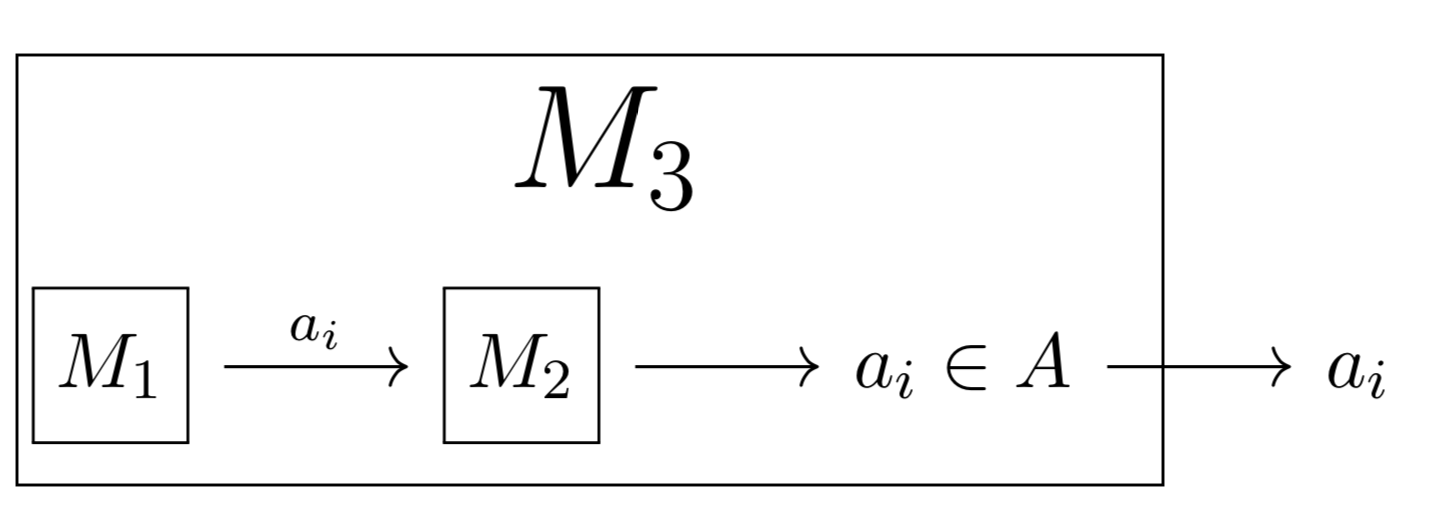
\includegraphics[scale = 0.25]{figures/fig33.png}

\begin{comment}
% https://tikzcd.yichuanshen.de/#N4Igdg9gJgpgziAXAbVABwnAlgFyxMJZABgBpiBdUkANwEMAbAVxiRAB124BHAIwgAewOgH0AjAF8QE0uky58hFGPJVajFm049+Q0QCYpMudjwEi+1dXrNWiEKKzS1MKAHN4RUADMAThABbJDIQHAgkFXVbNkdpWRA-QIjqMKRLKM17ThwYARxgAGUsAAIJR04sMGKAQWcJIA

\begin{tikzcd}
\sqbox{$a_1$} \arrow[r, "a_i"] & \sqbox{$a_2$} \arrow[r] & a_i\in A \arrow[r] & a_i
\end{tikzcd}
\end{comment}

\begin{theorem*}\label{enumequiv}
Sea $U$ efectivamente enumerable, sea $A\subseteq U$. $A$ es decidible si y solo si $A$ y $A^{\complement}$ son efectivamente enumerables.
\end{theorem*}
\begin{proof}\mbox{}
\begin{itemize}
    \item[($\Longrightarrow$)] Por la anterior proposición, al ser $A$ decidible, $A$ es efectivamente enumerable. Ahora bien, por ser $U$ también efectivamente enumerable, el algoritmo que, dado un elemento de la lista de $U$ que no esté en la de $A$ lo añade a una lista, enumera a $A^{\complement}$.
    \item[($\Longleftarrow$)] Sean $M_1$, $M_2$ que enumeran, respectivamente, a $A$ y $A^{\complement}$. Como, dado un elemento $u$ de la enumeración de $U$, $u \in A$ o $u \in A^{\complement}$, se sigue que $u$ será enumerado por $M_1$ o por $M_2$. Por tanto, el algoritmo $M_3$ que, decide si el elemento $u$ está en las enumeraciones dadas por $M_1$ y $M_2$ decide si $u$ está en $A$. Por tanto, $A$ es decidible.
\end{itemize}
\end{proof}

\begin{note}
Existen conjuntos efectivamente enumerables no decidibles. Una forma de entender esto es que si un conjunto $A$ es efectivamente enumerable por un algoritmo $M_1$, entonces hay un algoritmo $M_2$ que responde $a\in A$ si un elemento $a$ está en $A$: en efecto, basta con que este algoritmo ejecute los pasos de $M_1$ hasta que llegue al elemento $a$ de $A$, y entonces $M_2$ dice que  $a\in A$.

Sin  embargo, no tiene por qué haber un algoritmo que nos diga que un  elemento $b$ \textit{no} está en $A$: no podemos ejecutar el algoritmo $M_1$ durante `infinitos pasos' para  que compare $b$ a  todos los elementos de $A$ y deduzca que $b$ no está  en $A$. De ahí que en el teorema \ref{enumequiv} necesitemos  tanto  que $A$  como que $A^{\complement}$ sean efectivamente enumerables.
\end{note}

\subsection{Teorema de Enumeración}

Veamos los resultados que se siguen de las nociones que hemos introducido. 

Durante el resto de la sección \ref{teoyenum}, consideraremos una signatura $S$ y un conjunto de variables $Var$ que sean \textbf{efectivamente enumerables}. Esto nos permitirá usar, además de algunos resultados que hemos presentado en las secciones anteriores, los teoremas de corrección  y completitud.

\begin{lema*}\label{cosasenum}
Sea $S$ signatura efectivamente enumerable. Entonces:
\begin{itemize}
    \item $TERM_S$ es efectivamente enumerable.
    \item $FORM_S$ es efectivamente enumerable.
    \item $Sent_S$ es efectivamente enumerable.
\end{itemize}
\end{lema*}
\begin{proof}
Se omite.
\end{proof}

\begin{lema*}
Si $A$ es un conjunto efectivamente enumerable, $\mathcal{P}_{fin}A$, el conjunto de subconjuntos  finitos de $A$, también lo es.
\end{lema*}
\begin{proof}
Se omite.
\end{proof}

\begin{prop*}\label{arbenum}
Si la signatura $S$ es efectivamente enumerable, el conjunto de árboles de deducción de las fórmulas asociadas es efectivamente enumerable.
\end{prop*}
\begin{sketchproof}
Sabemos de los dos anteriores resultados que $Sent_S$ y $\mathcal{P}_{fin}(Sent_s)$ son efectivamente enumerables por los algoritmos $a_1$ y $a_2$, respectivamente. Tenemos por tanto las enumeraciones $a_1: \varphi_1, \varphi_2, \dots$ y $a_2: \Gamma_1, \Gamma_2, \dots$

Esbocemos el siguiente algoritmo, que consiste en un bucle. En la etapa $n$-ésima consideramos las secuencias del tipo $\Gamma_i \idash \varphi_j$, con $i, j \leq n$. A continuación, construimos todos los árboles de deducción de profundidad $\leq n$ que tienen por raíz a $\Gamma_i \idash \varphi_j$. Este conjunto es claramente finito.

De este modo, el conjunto de árboles de deducción es efectivamente enumerable.
\qed
\end{sketchproof}


\begin{definition}
Sea $S$ signatura. Dado $\Phi \subseteq FORM_S$, definimos la \textit{teoría de} $\Phi$ como:
$$Th(\Phi) := \{\varphi \in Sent_S \, \, | \, \, \Phi \vdash \varphi\}$$
\end{definition}

\begin{theorem*}(Teorema de Enumeración)
Sea $S$ signatura efectivamente enumerable. Si $\Phi \subseteq Sent_S$ es efectivamente enumerable, $Th(\Phi)$ es efectivamente enumerable.
\end{theorem*}


\begin{sketchproof}
Consideremos las enumeraciones respectivas de $\Phi$ y del conjunto de los árboles de deducción, $a_1: \varphi_1, \varphi_2, \dots$ y $a_2:A_1, A_2, \dots$.

Construyamos otro algoritmo con un bucle. En la etapa $n$-ésima consideramos los árboles de deducción ya enumerados, de modo que cada uno de los árboles $A_i$ tiene por raíz a una secuencia $\Gamma_i \idash \psi_i$, con $i \leq n$. De este modo, si $\Gamma_i \subseteq \{\varphi_1, \dots, \varphi_n\}$ y $A_i$ tiene axiomas en las hojas, incorporamos $\psi_i$ a nuestra enumeración.

Veamos que así conseguimos enumerar $Th(\Phi)$. Sea $\sigma \in Th(\Phi)$. Entonces, $\Phi \vDash \sigma$ y $\Phi \vdash \sigma$. De modo que existe $\Gamma \subseteq \Phi$ finito tal que $\vdash \Gamma \idash \sigma$. Por ser finito, tenemos que existen los enteros: (i) $k_1$ tal que $\Gamma \subseteq \{\varphi_1, \dots, \varphi_{k_1}\}$, (ii) $k_2$, que es la profundidad del árbol de deducción para $\vdash \Gamma \idash \sigma$ y (iii) $k_3$, que es la posición del árbol de deducción en la enumeración $a_2$.
Tomando $k = \max\{k_1, k_2, k_3\}$, enumeramos $\sigma$ en la etapa $k$-ésima del algoritmo que hemos descrito.\qed
\end{sketchproof}

\subsection{Teorías}

Cuando pensamos informalmente en una \textit{teoría}, solemos referirnos a un conjunto de principios básicos y a los resultados que se obtienen de ellos y/u otros resultados. Es decir, nos referimos a un conjunto de proposiciones que es \textit{cerrado bajo} consecuencia lógica. Esta misma idea es la que se tiene en la definición formal:

\begin{definition}
Sea $S$ signatura. $T \subseteq Sent_S$ es \textit{teoría} si para cada $\varphi$, si $T \vDash \varphi$ entonces $\varphi \in T$.
\end{definition}

\begin{example}
Dado $\Phi \subseteq Sent_S$, $Th(\Phi)$ es teoría.
\end{example}
\begin{example}
Dada $S$ signatura, $\mathfrak{A}$ $S$-álgebra, $Th(\mathfrak{A})$ es teoría. 
\end{example}

\begin{defs*}\mbox{}
\begin{itemize}
    \item Una teoría $T$ es \textit{finitamente axiomatizable} si existe $\Phi \subseteq Sent_S$ finito tal que $T=Th(\Phi)$.
    \item Una teoría $T$ es \textit{efectivamente axiomatizable} si existe $\Phi \subseteq Sent_S$ decidible tal que $T=Th(\Phi)$.
    \item Una teoría $T$ es \textit{completa} si para toda $\varphi \in Sent_S$, $\varphi \in T$ o $\neg \varphi \in T$.
\end{itemize}
\end{defs*}

\begin{lema}
Sea $S$ signatura. Una teoría $T \subseteq Sent_S$ es insatisfactible si y solo si $T = Sent_S$.
\end{lema}
\begin{proof}
$Sent_S$ es insatisfactible, ya que contiene por ejemplo a la fórmula $\exists x\neg x\doteq x$, con lo que esa implicación es trivial. Recíprocamente, si $T$ es insatisfactible, entonces para toda $\sigma \in Sent_S$, $T \vDash \sigma$, y por tanto $\sigma \in T$.
\end{proof}

\begin{prop}\label{complet}
Sean $S$ signatura, $\mathfrak{A}$ $S$-álgebra. Entonces:
\begin{enumerate}
    \item $Th(\mathfrak{A})$ es completa.
    \item Si la teoría $T$ es completa y $\mathfrak{A} \in Mod(T)$, entonces $T = Th(\mathfrak{A})$.
    \item $T$ es completa si y solo si para cualesquiera $\mathfrak{A}, \mathfrak{B} \in Mod(T)$, $\mathfrak{A} \equiv \mathfrak{B}$.
\end{enumerate}
\end{prop}
\begin{proof}\mbox{}
\begin{itemize}
    \item[(1)] Sea $\varphi \in Sent_S$. Si $\mathfrak{A}\vDash \varphi$, $\varphi \in Th(\mathfrak{A})$; si $\mathfrak{A} \nvDash \varphi$, entonces $\mathfrak{A} \vDash \neg \varphi$ y $\neg \varphi\in Th(\mathfrak{A})$.
    \item[(2)] Sea $\mathfrak{A} \in Mod(T)$, entonces $\mathfrak{A}$ verifica todo elemento de $T$, por tanto $T \subseteq Th(\mathfrak{A})$. Por otro lado, si $\varphi \in Th(\mathfrak{A})$, entonces $\mathfrak{A} \vDash \varphi$, $\mathfrak{A} \nvDash \neg \varphi$ y $\neg \varphi \notin Th(\mathfrak{A})$, de lo que se sigue que $\neg\varphi \notin T$ y $\varphi \in T$.
    \item[(3)] Si $T$ es completa y $\mathfrak{A}, \mathfrak{B} \in Mod(T)$ entonces, por el apartado (2), $Th(\mathfrak{A}) = T = Th(\mathfrak{B})$, de lo que se sigue que $\mathfrak{A} \equiv \mathfrak{B}$.
    
    Veamos la implicación recíproca. Supongamos que $T$ no es completa, es decir, existe $\varphi \in Sent_S$ tal que $\varphi, \neg\varphi \notin T$. Al ser $T$ teoría, $T \nvDash \varphi, \neg\varphi$ y por tanto existen dos $S$-estructuras $\mathfrak{A}, \mathfrak{B} \in Mod(T)$ tales que $\mathfrak{A} \nvDash \varphi$ y $\mathfrak{B}\nvDash \neg\varphi$. Pero entonces $\mathfrak{B}\vDash \varphi$, con lo que $\varphi \notin Th(\mathfrak{A})$ y $\varphi \in Th(\mathfrak{B})$. Ergo, $Th(\mathfrak{A})\neq Th(\mathfrak{B})$, es decir, $\mathfrak{A} \not\equiv \mathfrak{B}$.
\end{itemize}
\end{proof}

En lo que queda de sección vamos a probar las siguientes implicaciones, siendo $T$ una teoría:

\begin{center}
\tikzset{every picture/.style={line width=0.75pt}} %set default line width to 0.75pt        

\begin{tikzpicture}[x=0.75pt,y=0.75pt,yscale=-1,xscale=1]
%uncomment if require: \path (0,110); %set diagram left start at 0, and has height of 110


% Text Node
\draw (55,7) node [anchor=north west][inner sep=0.75pt]   [align=left] {$\displaystyle T\ decidible$};
% Text Node
\draw (84.01,31) node [anchor=north west][inner sep=0.75pt]  [rotate=-90.00] [font=\large, align=left] {$\displaystyle \Longrightarrow $};
% Text Node
\draw (96,60) node [anchor=north west][inner sep=0.75pt]  [rotate=-270.00] [font=\large, align=left] {$\displaystyle \Longrightarrow $};
% Text Node
\draw (117,40) node [anchor=north west][inner sep=0.75pt]  [font=\scriptsize] [align=left] {$\displaystyle {\displaystyle T\ completa}$};
% Text Node
\draw (3,73) node [anchor=north west][inner sep=0.75pt]   [align=left] {$\displaystyle T\ efectivamente\ enumerable$};
% Text Node
\draw (195,70) node [anchor=north west][inner sep=0.75pt]   [font=\large, align=left] {$\displaystyle  \begin{array}{{>{\displaystyle}l}}
\Longleftrightarrow \\
\end{array}$};
% Text Node
\draw (263,73) node [anchor=north west][inner sep=0.75pt]   [align=left] {$\displaystyle T\ efectivamente\ axiomatizable$};
% Text Node
\draw (268,3) node [anchor=north west][inner sep=0.75pt]   [align=left] {$\displaystyle T\ finitamente\ axiomatizable$};
% Text Node
\draw (354,31) node [anchor=north west][inner sep=0.75pt]  [rotate=-90] [font=\large, align=left] {$\displaystyle \Longrightarrow $};
% Text Node
\draw (366,60) node [anchor=north west][inner sep=0.75pt]  [rotate=-270] [font=\large,align=left] {$\not\Longrightarrow$};


\end{tikzpicture}
\end{center}

\begin{theorem*}
Sea $S$ signatura, $T$ teoría. $T$ es efectivamente axiomatizable si y solo si es efectivamente enumerable.
\end{theorem*}
\begin{proof}\mbox{}
\begin{itemize}
    \item[($\Longrightarrow$)] Si $T$ es efectivamente axiomatizable, existe $\Phi \subseteq Sent_S$ decidible tal que $Th(\Phi) = T$. Por \ref{arbenum} tenemos  un algoritmo que enumera los árboles de deducción, $a_1: A_1, A_2, \dots$.\\

Construyamos ahora un procedimiento que enumere $T$. Para ello, nos basta encontrar todas las fórmulas $\varphi$ tales que existe un árbol de deducción en cuya raíz hay una secuencia $\Gamma\idash\varphi$, con $\Gamma\subseteq\Phi$ finito. En cada etapa $n$, consideramos el árbol $A_n$, cuya raíz llamamos $\Gamma_i \idash \varphi_i$. Se comprueba:
\begin{itemize}
    \item Si $A_i$ tiene axiomas en las hojas, lo que se puede comprobar de manera efectiva ya que se puede comprobar que el conjunto de axiomas es decidible.
    \item Si $\Gamma_i \subseteq \Phi$, lo que es posible comprobar mediante un algoritmo, por ser $\Gamma_i$ finito y $\Phi$ decidible (basta ir tomando cada elemento de $\Gamma_i$ y decidiendo si se encuentra o no en $\Phi$).
\end{itemize}

Y en caso de que se cumplan ambas condiciones, añadimos $\varphi$ a $T$.

    \item[($\Longleftarrow$)] Al ser $T$ efectivamente enumerable, tenemos un algoritmo que lo enumera, $a_2: \varphi_1, \varphi_2, \dots$. Llamando $\psi_n=\bigwedge_{i_1}^n\varphi_i$, sea $\Phi := \{\psi_n\}_{n\in\mathbb{N}}$. Nos bastará con demostrar que $\Phi$ es decidible y que $T=Th(\Phi)$. Comencemos viendo que $T = Th(\Phi)$:
    \begin{itemize}
        \item $T\subseteq Th(\Phi)$: Dada $\varphi \in T$, existe cierto $n$ entero positivo tal que $\varphi = \varphi_n$. Por tanto, $\psi_n \vDash \varphi$ y entonces $\varphi \in Th(\Phi)$.
        \item $Th(\Phi)\subseteq T$: Sea $\varphi\in Th(\Phi)$. Esto implica que $\Phi\vDash\varphi$. Por el teorema de compacidad, hay un subconjunto finito $\Gamma\subseteq\Phi$ tal  que $\Gamma\vDash\varphi$. Si la última fórmula de $\Phi$ que está en $\Gamma$ es $\psi_k$, entonces $\Gamma\subseteq\{\psi_1,\dots,\psi_k\}$. Por tanto, $\{\psi_1,\dots,\psi_k\}\vDash\varphi$.\\
        
        Pero sabemos que $T\vDash\psi_i$ para todo $i$, ya que $T\supseteq\varphi_1,\dots,\varphi_i\vDash\psi_i$. Por tanto, como $T\vDash\{\psi_1,\dots,\psi_k\}$, tenemos que $T\vDash\varphi$, y como  $T$ es una teoría, $\varphi\in T$.
    \end{itemize}
    Veamos ahora que $\Phi$ es decidible. Como $\psi_i=\varphi_1\land\dots\land\varphi_i$, la longitud de $\psi_i$ es $\geq i$ para todo $i$.\\
    
    Ahora, sea $\chi\in Sent_S$ cualquiera de longitud $l$. Ponemos en marcha el algoritmo que enumera $T$, y en el paso $n$ comprobamos si $\chi=\varphi_1\land\dots\land\varphi_n$. Si en para algún $n$ se cumple esta igualdad, hemos acabado, $\chi\in\Phi$. Si llegamos a $n=l+1$ y no se ha cumplido la igualdad en ningún paso, acabamos el algoritmo y concluímos que $\chi\notin\Phi$, ya que hemos comprobado que $\chi\neq\psi_n$ para $n=1,\dots,l$ y además $\chi\neq\psi_n$ para $n>l$, ya que la longitud de $\chi$ es $l$ y la longitud de $\psi_n$ es $>l$.
\end{itemize}
\end{proof}

\begin{prop*}
Sea $S$ signatura, $T$ teoría. Si $T$ es efectivamente enumerable y completa, entonces es decidible.
\end{prop*}
\begin{proof}
Si $T$ es insatisfactible, entonces $T = Sent_S$ y por tanto es decidible. Supongamos entonces que $T$ es satisfactible.

Al ser efectivamente enumerable, existe el algoritmo $a_1: \varphi_1, \varphi_2, \dots$. Sea $\psi \in Sent_S$. Entonces, por ser $T$ completa, $\psi \in T$ o $\neg\psi \in T$. Por tanto, en la enumeración que da $a_1$, terminaremos encontrando $\psi$ o $\neg \psi$, lo que nos permite decidir si $\psi$ está o no en $T$.
\end{proof}

\begin{example}
Veamos un ejemplo de teoría efectivamente axiomatizable pero no finitamente axiomatizable.

Consideremos el conjunto $\Phi_{C_0}$ de los axiomas de cuerpos de característica 0. Entonces $\Phi_{C_0}$ es decidible (es fácil) y por tanto $T := Th(\Phi_{C_0})$ es efectivamente axiomatizable, pero veamos que no es finitamente axiomatizable.

Si fuera finitamente axiomatizable, $T=Th(\{\varphi_1,\dots,\varphi_n\})$, entonces tendríamos que la fórmula $\varphi=\varphi_1\land\dots\land\varphi_n$ se cumple exactamente en los cuerpos de característica 0. Pero esto significaría que $\neg\varphi$ se cumpliría en los cuerpos de característica finita (de hecho, en cualquier estructura que no fuera un cuerpo de característica 0). Sin embargo, se puede demostrar de forma similar a \ref{fintoinf} que si un conjunto de fórmulas tiene de modelos cuerpos de característica arbitrariamente grande, entonces tiene de modelo algún cuerpo de característica 0, de modo que tenemos una contradicción.
\end{example}

\section{Categoricidad}

Finalizamos este capítulo con uno de los conceptos más importantes de Teoría de Modelos. 

La noción de categoricidad viene motivada por el papel que juegan las teorías respecto de los objetos que tratan. Es decir, a simple vista, una teoría puede tener diversos modelos, y los axiomas que la componen parecen no describir más que la forma en que se comportan ciertos elementos. Sin embargo, existen teorías de las cuales solo existe un modelo salvo isomorfismo y, por tanto, en estos casos sí que podemos afirmar que los axiomas \textit{caracterizan} los objetos que estudian. Esto queda condensado en la siguiente 

\begin{definition}
Sea $S$ signatura. Una teoría $T$ se dice \textit{categórica} si $\mathfrak{A} \approx \mathfrak{B}$ para cualesquiera $S$-álgebras $\mathfrak{A}, \mathfrak{B} \in Mod(T)$. 
\end{definition}

\begin{prop}
Sea $S$ signatura efectivamente numerable, $T$ teoría. Si $T$ es categórica, es completa.
\end{prop}
\begin{proof}
Sean $\mathfrak{A}, \mathfrak{B} \in Mod(T)$ $S$-álgebras. Entonces, por categoricidad, $\mathfrak{A} \approx \mathfrak{B}$, y por tanto, $\mathfrak{A} \equiv \mathfrak{B}$. Como esto se cumple para cualesquiera $\mathfrak{A}, \mathfrak{B} \in Mod(T)$, por \ref{complet} $T$ es completa.
\end{proof}

\begin{prop}\label{infnocat}
Sea $S$ signatura, sea $T$ teoría. Si $T$ tiene modelos infinitos, no es categórica.
\end{prop}
\begin{proof}
Sea la $S$-álgebra infinita $\mathfrak{A}\vDash T$ y llamamos $\kappa= |\mathfrak{A}|$. Por ser $\kappa$ infinito, \ref{noiso} nos dice que existe una $S$-álgebra $\mathfrak{A}^{*}$ no isomorfa a $\mathfrak{A}$ y tal que $\mathfrak{A} \equiv \mathfrak{A}^{*}$. Por tanto, $\mathfrak{A}^{*} \vDash T$, y $T$ no es categórica.
\end{proof}

Esta es una proposición bastante sorprendente que nos hace darnos cuenta de las limitaciones de la lógica de primer orden. Nos dice que cualquier estructura infinita en la que pensemos, por ejemplo los naturales $\mathbb{N}$ con su buen orden, el grupo de los enteros $\mathbb{Z}$, o el cuerpo ordenado $\mathbb{R}$, ninguna de ellas puede \textit{caracterizarse} mediante axiomas de primer orden.

\begin{definition}
Sea $S$ signatura. Una teoría $T$ se dice $\kappa$-\textit{categórica} si $\mathfrak{A} \approx \mathfrak{B}$,  para cualesquiera $S$-álgebras $\mathfrak{A}, \mathfrak{B} \in Mod(T)$ tales que $|\mathfrak{A}|= |\mathfrak{B}| = \kappa$.
\end{definition}

\begin{theorem}
Sea $S$ signatura efectivamente numerable. Si $T$ es una teoría satisfactible, sin modelos finitos y $\kappa$-categórica para algún cardinal $\kappa \geq|\mathbb{N}|=\omega$, entonces es completa.
\end{theorem}
\begin{proof}
Supongamos que $T$ no es completa. Entonces existe $\sigma \in Sent_S$ tal que $\sigma, \neg\sigma \notin T$, es decir, tal que $T \nvDash \sigma, \neg\sigma$ y entonces $T\cup\{\sigma\}$ y $T\cup\{\neg\sigma\}$ son satisfactibles y por \ref{LST} existen dos $S$-álgebras $\mathfrak{A}, \mathfrak{B}$ tales que $\mathfrak{A}\vDash T\cup \{\sigma\}$ y $\mathfrak{B}\vDash T\cup\{\neg\sigma\}$ y de modo que $\kappa = |\mathfrak{A}| = |\mathfrak{B}|$. Entonces, al ser $\mathfrak{A} \vDash T$ y $\mathfrak{B} \vDash T$, y por $\kappa$-categoricidad, $\mathfrak{A} \approx \mathfrak{B}$, lo que es imposible, ya que $\mathfrak{A}\vDash \sigma$ y $\mathfrak{B}\vDash \neg\sigma$.
\end{proof}




\begin{comment}
\begin{example}
Consideremos la signatura $S := \langle \emptyset; \emptyset; R|_2\rangle$. Consideremos los axiomas de un orden lineal sin puntos extremos, $\Phi$, y sea $T:=Th(\Phi)$. Veamos que es una teoría $\omega$-categórica.

Sea $Q := \langle \Q, \leq \rangle$ de modo que, claramente, $\Q \vDash T$. Sea $\mathfrak{A} := \langle A, R^{\mathfrak{A}}\rangle$ tal que $\mathfrak{A} \vDash T$. Supongamos que $|\Q| = |A| = \omega$. Entonces, por ser ambos numerables, existe una biyección de uno en el otro(???????????????)
\end{example}
\end{comment}

\appendix
%    Include appendix "chapters" here.


%    Bibliography styles amsplain or harvard are also acceptable.
\bibliographystyle{amsalpha}
%    See note above about multiple indexes.
\printindex

\end{document}

%-----------------------------------------------------------------------
% End of amsbook-template.tex
%-----------------------------------------------------------------------
